%% MoCHII — gas physics, atomic data, algorithms, and validation.
%% Author: Kwang-Il Seon
%% Written 2026-07-12 for my_memo.cls.
\documentclass[english,a4paper]{my_memo}
\synctex=1
\usepackage{amsmath}
\usepackage{amssymb}
\usepackage{microtype}
\usepackage{booktabs}
\usepackage{longtable}

\newcommand{\code}[1]{\texttt{#1}}
\newcommand{\cmc}{\mathrm{cm^{3}\,s^{-1}}}
\newcommand{\xHI}{x_{\mathrm{HI}}}
\setlength{\emergencystretch}{2em}

\begin{document}

\title{MoCHII: Physics, Atomic Data, Algorithms, and Validation}
\author{Kwang-Il Seon}
\date{\docmoddate}
\maketitle

\begin{abstract}
MoCHII (MOnte Carlo for H\,\textsc{ii} regions) adds a photoionization gas
layer to the validated octree-AMR dust radiative-transfer engine of MoCafe
v2.00.  This memo documents the
ionizing frequency band and its zero-variance transport, the complete
atomic-data inventory with sources and the analytic fitting functions
evaluated at run time, the iteration and equilibrium algorithms
(ionization, thermal balance, trace-metal cascade, explicit diffuse
field), the $n$-level emissivity solver, the ported nebular
continuum and Storey \& Hummer recombination lines, and the
quantitative validation gates: rate
integrals vs.\ analytic attenuation (bias $+0.004\%$); the Str\"omgren
sphere vs.\ an exact 1D reference ($+1.01\%$ in the ionized-volume radius at level 6, $+0.69\%$ at level 7; AMR
$\equiv$ uniform); the thermal H/He nebula (median $0.12\%$ in $T_e$);
the MOCASSIN Lexington benchmarks ($T_e = 8176$~K at HII40 and 6942~K at
HII20 with the density-suppressed cooling default, run to the drift stopping
test, matching a current \textsc{Cloudy} c25.00 run to $-0.41\%$ and $+0.46\%$,
with the HII40 He\,\textsc{i} front $0.025$~pc inside \textsc{Cloudy}'s; the
zero-density limit gave 7877 and 6282~K, m11, not rerun under the
2026-10-11 physics); and the line-flux comparison
($L({\rm H}\beta)$ inside the published range at both, the optical
collisional lines within the published spread).
Also documented: the solution-driven I-front re-refinement
(re-refined vs.\ native high-resolution octree $+0.012\%$ in the
ionized-volume radius with $4.5\times$ fewer cells) and an Illustris-TNG
post-processing demonstration; the completed dust coupling
(ionizing-band dust absorption with the dusty Str\"omgren reduction
0.724 reproduced to $+0.34\%$; EUV/FUV dust \emph{scattering} with
forced-first interaction sampling, validated by bracketing; live
ionization-dependent dust with a PAH-specific survival factor; and the
equilibrium dust temperature + IR spectrum consuming the transported
grain heating, energy closure 1.000); and the incremental metal
additions (argon, magnesium, iron, and silicon/chlorine/calcium) as
pure data operations.
\end{abstract}

\begin{sloppypar}
\noindent\textbf{Current state (2026-10-11).}
The plan in force restores the physics of the last committed version and
extends it to the process scope of MOCASSIN v2 at current data
(\code{md/ATOMIC\_PHYSICS\_RESTORATION\_PLAN\_2026-10-11.md}; results in
\code{md/ATOMIC\_PHYSICS\_RESTORATION\_RESULTS\_2026-10-11.md}).
\begin{itemize}\itemsep1pt
\item \emph{Stages:} I--VII of all eleven metals, 77 stages and 66
  transitions (\S\ref{sec:cascade}).  A band reaching above the ionization
  potential of the last carried stage of an element present is refused; the
  lowest is Cl\,\textsc{vii}, 114.2~eV.
\item \emph{Photoabsorption:} the \code{phfit2} subshell sum at every
  energy, with the Nahar (2019) R-matrix ground-term table for
  Ne\,\textsc{iii} (\S\ref{sec:photo}).
\item \emph{Excitation atoms:} \code{metal\_excitation\_model = 'chianti'}
  (the default) takes full CHIANTI 11.0.2 atoms for 67 stages and Stout
  atoms for Cl\,\textsc{vii}, Ar\,\textsc{ii}, Ca\,\textsc{iv}: 70 atoms,
  6629 levels, 70 cooling fits, 482 terms.  \code{'mocassin\_v2'} takes the
  MOCASSIN v2 atoms (55 atoms, 571 levels, 49 fits, 788 terms) for parity
  runs.  Every stage with an atom cools and emits (\S\ref{sec:cool},
  \S\ref{sec:nlev}).
\item \emph{On by default:} metal collisional ionization, atomic-hydrogen
  impact on the C\,\textsc{i}, C\,\textsc{ii}, O\,\textsc{i} fine structure,
  charge-exchange heating, the He\,\textsc{i} 2$^3$S coupling, the FUV band
  from 4.78~eV whenever He\,\textsc{i} 2$^3$S, a metal with an edge below
  13.6~eV, or dust is present, the metal ground free--bound and the
  free--free diffuse channels 6 and 7 (\S\ref{sec:metalcont}), and, with
  dust, Weingartner \& Draine (2001) grain photoelectric heating and
  Hollenbach \& McKee (1979) gas--grain exchange (\S\ref{sec:pdr}).
\item \emph{Removed and refused} with their replacement named:
  \code{metal\_inner\_shell\_absorption}, \code{additional\_line\_cooling},
  \code{high\_charge\_exchange} (now \code{langevin\_charge\_exchange}),
  \code{fe\_levels\_full}, \code{pe\_scale}, and
  \code{metal\_excitation\_model = 'extended'}
  (\code{setup.f90::refuse\_removed\_items}).
\end{itemize}
Measurements in this memo carry their dates.  The converged Lexington
benchmarks were rerun on this state
(\code{results/\allowbreak continuous\_energy/\allowbreak m13\_restoration/},
restarted from \code{m11\_hecx\_solver}, 29 and 26 iterations to the drift
test; \S\ref{sec:hii}); the PN150 run converged on 2026-10-14 without
metal recombination radiation in the diffuse field (\S\ref{sec:limits}).  Variants not
rerun (the zero-density cooling, on-the-spot, low-density and no-He--H
charge-exchange runs) keep their m11 values, marked as such.
\end{sloppypar}

\tableofcontents

%==========================================================================
\section{Scope and design rules}
MoCHII copies validated modules from MoCafe v2.00 (octree, event-driven
traversal, MPI shared memory, HDF5/FITS I/O) and adds gas microphysics
under three design rules:
(1) \emph{atomic data are fitted offline, evaluated online} --- the Python
fitting code under \code{tools/fitting/} is the auditable source of every
coefficient in \code{data/atomic/}, and Fortran only evaluates closed
forms; (2) \emph{adding an ion is a data operation}, realized by the
species registry (Section~\ref{sec:cascade}); (3) \emph{validation by
quantitative gates}, each capability compared against an analytic or
external reference.

The capabilities documented here: the ionizing band + rate integrals;
ionization equilibrium + opacity feedback (case B, fixed $T_e$);
thermal balance + trace-metal frame; the explicit diffuse field
(case A); solution-driven I-front re-refinement + snapshot
post-processing; the dust coupling (absorption competition,
scattering, live PAH split, grain heating/temperature, and the SEDust
stochastic-emission coupling); the incremental ions (argon,
magnesium, iron, silicon, chlorine, calcium); plus the output-time
diagnostic layer: $n$-level emissivities, Storey \& Hummer
recombination lines, and the nebular continuum.

%==========================================================================
\section{The ionizing band and transport}
\subsection{Continuous energy and diagnostic bins}
\label{sec:band}
The ionizing band covers photon energies
$[E_{\min}, E_{\max}] = [13.598, 100]$~eV.  A packet energy is sampled
from the normalized source-energy CDF, never from a frequency bin (there is
no binned-energy mode).
For a Planck source the CDF is built adaptively from the Planck energy
spectrum; for a tabulated source it is the cumulative integral of the
input $L_E$.  H\,\textsc{i}, He\,\textsc{i}, He\,\textsc{ii}, and active
metal thresholds are retained as knots in the adaptive Planck CDF.  With
$u\in[0,1)$, the draw is
\begin{equation}
 F_E(E) = \frac{\int_{E_{\min}}^E L_{E'}\,{\rm d}E'}
                {\int_{E_{\min}}^{E_{\max}} L_{E'}\,{\rm d}E'},
 \qquad E_{\rm pkt}=F_E^{-1}(u), \qquad
 L_{\rm pkt}=\frac{L_{\rm band}}{N_{\rm pkt}} .
 \label{eq:band-source-cdf}
\end{equation}
Here $L_{\rm band}$ is the luminosity integrated over the whole ionizing
band, not the luminosity of one energy interval.  Each packet is therefore
an equal-luminosity sample of the source spectrum.

The packet retains $E_{\rm pkt}$ throughout transport.  Gas opacity,
photoionization cross sections, and the excess energy used for heating are
evaluated at this exact energy.  The $n_\nu$ bins
(\code{par\%nnu\_ion}, default 16; gates use 32) receive only a diagnostic
$J_E$ tally, which is kept only when \code{par\%jnu\_output} asks for it to
be written (default off) or the SEDust emission reads it: the sampled energy
is located by a binary search of the bin-edge array and assigned an output
index.  Consequently the number or placement of those bins cannot alter the
physical solution; it changes only the spectral resolution of the saved
tally.  This is
important at thresholds: a photon exactly on a stored edge is assigned to
the bin above it, but its interaction physics still uses its own energy.

Every source configuration is sampled this way: one or several internal
point sources, an external isotropic field, plane-parallel slab
illumination, and the analytic ISRF presets, each drawing from its own
spectrum through its own inverted CDF.

\paragraph{Diagnostic bin edges.}  \code{par\%ion\_align\_edges} (default
on) pins the ionizing-band bin edges onto the ionization thresholds --- H\,\textsc{i}
(13.6~eV), He\,\textsc{i} (24.6~eV), He\,\textsc{ii} (54.4~eV), plus the
active metal photoionization thresholds gathered from the registry ---
so that no bin straddles a threshold.  The sub-segments between
consecutive thresholds are log-uniform, and bins are distributed among
the segments by log width (largest-remainder, floor 1).  When the
thresholds outnumber the bins the lowest-priority (metal) edges are
dropped gracefully --- the H/He edges are always kept --- so the option
is safe at any \code{nnu\_ion}.  Setting it \code{.false.} uses a
single log grid.  Because the transported energies are continuous, this
choice changes the resolution of the saved $J_E$ tally only; it cannot move
the physical solution.

\paragraph{FUV extension.}  With \code{par\%add\_fuv} the band grows a
second, lower segment: \code{par\%nnu\_fuv} log bins on
$[E_{\rm FUV}, E_{\min}]$ (\code{par\%efuv\_min}; left out of the input, 4.78~eV by the rule below, or 6~eV when nothing in the run absorbs below 13.6~eV)
\emph{below} the unchanged ionizing bins, so widening the band does not
coarsen the ionizing resolution (the earlier single-segment caveat).
\code{par\%luminosity} keeps its meaning as the ionizing
$[E_{\min}, E_{\max}]$ luminosity; the FUV part of the same source
spectrum rides on top ($L_{\rm FUV}/L_{\rm ion} = 1.097$ for a
4$\times$10$^4$~K Planck source at 6~eV), so the ionizing photon budget
$Q_{\rm H}$ is preserved without manual band-ratio rescaling.  How the
packets are shared between the two segments is \code{par\%fuv\_sampling}
(Section~\ref{sec:band-strata}): by default each segment is a stratum with
its own packet count, and a packet carries its stratum's luminosity over
that count; \code{'proportional'} draws every packet from one CDF over the
whole band, with $L_{\rm pkt} = (L_{\rm ion} + L_{\rm FUV})/N$.  An input
that leaves \code{add\_fuv} and \code{efuv\_min} out gets the extension
from 4.78~eV whenever something in the run absorbs below the hydrogen
edge: the He\,\textsc{i} 2$^3$S population (\code{hei\_metastable\_coupling},
on by default, or \code{hei\_metastable}, with helium), whose
photoionization rate is scored from this band
(Section~\ref{sec:hei-phi3}); a metal whose neutral ionization potential
lies below 13.598~eV (C, S, Mg, Fe, Si, Cl, Ca); or dust
(\code{ion\_add\_dust}), whose heating and photoelectric emission this band
drives (since 2026-10-11; before, the He\,\textsc{i} 2$^3$S population
alone set it, and otherwise the default was no extension from 6~eV).
4.78~eV is below every metal edge (Ca\,\textsc{i} 6.11~eV).  H and He cross
sections vanish below their thresholds, so the FUV bins interact only
with dust and with the low-threshold metal stages (next subsection) ---
they penetrate the neutral gas beyond the I-front and photoionize
Mg\,\textsc{i} (7.65~eV), C\,\textsc{i} (11.26~eV), S\,\textsc{i}
(10.36~eV), and Fe\,\textsc{i} (7.90~eV) there, producing the
PDR-side Mg\,\textsc{ii} and C\,\textsc{ii} that the
ionizing-only band cannot.

\subsection{Source components: multiple point sources and an external
field}
\label{sec:sources}
The band is fed by any number of \emph{source components}:
\code{par\%nsource} internal point sources (0--16; positions
\code{par\%src\_x/y/z}, ionizing luminosities \code{par\%src\_lum} ---
all set, or none for an equal split of \code{par\%luminosity}, which
becomes the sum) plus, independently, one isotropic external radiation
field, on when \code{par\%ext\_intensity} $> 0$.  Each packet draws a
component in proportion to its band-total luminosity, is emitted from
it, and draws its energy from that component's own spectrum CDF;
every packet carries $L_{\rm pkt} = \sum_c L_c/N$.  A single-component
run takes the legacy code path (the RNG stream is unchanged, so earlier
results reproduce).  The spectrum of internal source $i$ resolves as
\code{par\%src\_spectrum\_file} column $i$ $>$ \code{src\_tstar}$(i)$
Planck $>$ the global \code{ion\_spectrum} file $>$ the global
\code{tstar}; \code{src\_spectrum\_file} is one multi-column text file
--- column 1 the photon energy $E$ [eV] ascending, then one $L_E$
column for each source in arbitrary units, each independently
normalized so source $i$'s ionizing segment carries
\code{src\_lum}$(i)$.

The external field is an isotropic band-integrated mean intensity $J$
[erg\,s$^{-1}$\,cm$^{-2}$\,sr$^{-1}$] entering through an illuminating
surface (\code{par\%ext\_geometry}): \code{'rec'}, the box faces
(face-area-weighted --- correct for a non-cubic box), or \code{'sph'},
the bounding sphere of radius \code{par\%rmax} about the box center.
The inward flux through the surface is the hemisphere integral of
$J\cos\theta$, so the entering band power is
\begin{equation}
  F_{\rm in} = \int_{2\pi} J\cos\theta\,d\Omega = \pi J,
  \qquad
  L = \pi J A_{\rm surf}.
  \label{eq:extlum}
\end{equation}
Entry directions are cosine-weighted (Lambert) into the inward
hemisphere, $\mu = \sqrt{\xi}$, which reproduces an isotropic interior
field with energy density $u = 4\pi J/c$: an optically thin box tallies
an interior mean intensity equal to $J$ (the gate of
Section~\ref{sec:extval}).  Its spectrum resolves as
\code{ext\_spectrum} (file) $>$ \code{ext\_tstar} Planck $>$
the global spectrum.

\paragraph{Physical-unit spectra.}  Every file slot is read in the
column units set by \code{par\%spectrum\_type} (default \code{'shape\_ev'},
arbitrary units renormalized to the scale --- the legacy behavior).  The
physical types \code{'per\_ev'}, \code{'per\_hz'}, \code{'per\_ang'},
\code{'per\_um'} give the first column as $E$ [eV], $\nu$ [Hz], or
$\lambda$ [\AA{} or $\mu$m] and the value columns as a luminosity
density $L_X$ (internal sources) or an intensity density $J_X$ (external
field) in the matching spectral unit; wavelength tables are converted to
energy and sorted.  The \code{'shape\_ev'} value columns are read as the
density per eV $L_E$ on the $E$~[eV] grid; a shape tabulated in
wavelength or frequency must use the matching \code{per\_*} type, whose
conversion applies the $\mathrm{d}\lambda/\mathrm{d}E$ (or
$\mathrm{d}\nu/\mathrm{d}E$) Jacobian, so a raw re-grid onto $E$ under
\code{'shape\_ev'} would be wrong by $E^{-2}$.  A physical spectrum is
\emph{absolute}: its bin
luminosities follow the tabulated integral directly.  If the scale
(\code{luminosity} / \code{src\_lum}$(i)$ / \code{ext\_intensity}) is
unset it is derived from the file and reported; if set, the spectrum is
rescaled to it and acts as a shape.  With \code{add\_fuv} the same table
fills the FUV bins with no separate normalization; a spectrum with no
luminosity inside the band aborts.

\paragraph{ISRF presets.}  \code{par\%ext\_spectrum} may instead name one
of three analytic interstellar radiation fields: \code{'draine'}
(Draine 1978), \code{'habing'} (the Draine shape at Habing 1968
normalization, $/1.71$), and \code{'mathis'} (Mathis, Mezger \&
Panagia 1983), the shape of the SEDust radiation-field module.  They
are FUV-only (5~eV up to the H\,\textsc{i} edge, 13.598~eV, and exactly
zero in the ionizing band), so they
require \code{add\_fuv}, and \code{par\%ext\_scale} multiplies them.  The
Draine field is the energy-weighted photon polynomial
$F_{\rm ph}(E) = 1.658{\times}10^{6}\,E^{2} - 2.152{\times}10^{5}\,E^{3}
+ 6.919{\times}10^{3}\,E^{4}$ with $J_E = e\,F_{\rm ph}$
($e = 1.602{\times}10^{-12}$~erg\,eV$^{-1}$; $F_{\rm ph} = E\,N(E)$ is
energy-weighted --- a common pitfall).  The presets carry the canonical
FUV energy densities $u_{\rm FUV} = 8.94$, $5.23$,
$6.01{\times}10^{-14}$~erg\,cm$^{-3}$ (Draine / Habing / Mathis;
$G_0 = 1.69$, $0.99$, $1.14$ in Habing units).  When \code{ext\_intensity}
is set the preset or physical file is rescaled to that band-integrated
$J$ (a note is printed; \code{ext\_scale} is then ignored).

\subsection{Opacity and the zero-variance edge walk}
A packet of energy $E$ sees in a leaf the absorption coefficient per code
length
\begin{equation}
  \kappa(E) \;=\; n_{\rm H}\left[ \xHI\,\sigma_{\rm HI}(E)
   + y_{\rm He}\left( x_{\rm HeI}\sigma_{\rm HeI} +
     x_{\rm HeII}\sigma_{\rm HeII}\right)(E)\right] d_{\rm cm}
   \;(+\;\kappa_{\rm dust}(E)),
  \label{eq:packet-opacity}
\end{equation}
evaluated at the packet's own energy (\code{ion\_packet\_mod}): the cross
sections are computed once when the packet is launched
(\code{build\_ion\_packet\_physics}) and combined with the leaf state at each
step (\code{ion\_packet\_opacity}).  No opacity is stored for each energy
bin; the leaf carries only its state and the gray dust extinction density
\code{rhokap}, which the dust term multiplies by the packet's
$s_{\rm abs}(E)$ (and $s_{\rm sca}(E)$ when scattering is sampled;
\S\ref{sec:dust}).
With \code{par\%ion\_metal\_abs} (default on when \code{use\_metals})
the registry metals join the absorption,
$\Delta\kappa(E) = n_{\rm H}\sum_{\rm el} A_{\rm el} \sum_i
f_i\,\sigma_i(E)\,d_{\rm cm}$ (\code{species\_cached\_opacity}), with
$\sigma_i$ the cross section of
\S\ref{sec:photo} (Verner's \code{phfit2} subshell sum), the stage fractions $f_i$ from the same product chain as the
cooling, iterated by the opacity feedback exactly like $\xHI$.  Above
13.6~eV this is a $\sim$10$^{-22}$~cm$^2$ per H perturbation next to H/He
and dust; below 13.6~eV (the FUV extension) it is the only \emph{gas}
opacity.  The absorbed
share returns to the metals through their own $\Gamma$ integrals, so the
bookkeeping stays consistent, and the photoelectron energy it carries
enters the thermal balance under \code{par\%metal\_heat} (on by default)
through the shell-resolved heating coefficient of \S\ref{sec:photo}.

Where the band has no scattering, every packet's contribution to the
path estimators is computed \emph{analytically} along its ray (the
forced-first-flight estimator of MoCafe, made exact): in each leaf it
crosses the packet contributes the effective path length
\begin{equation}
  \ell_{\rm eff}({\rm leaf}) \;=\;
  \frac{e^{-\tau_{\rm in}} - e^{-\tau_{\rm out}}}{\kappa(E)},
  \label{eq:edgewalk}
\end{equation}
weighted by $w\,L_{\rm pkt}$, accumulated leaf by leaf until the domain
edge (\code{raytrace\_ion\_to\_edge\_amr}).  No interaction sampling is
needed; the only Monte Carlo variance is in the sampled energies and
directions.  The rate-integral gate verifies this estimator to a mean bias
of $+0.004\%$.

\subsection{Rate integrals}
With $V$ the leaf volume, the code forms for each absorber $i$ the path
estimators (\code{ion\_score\_mod}), summed over every packet segment
through the leaf and reduced over the MPI ranks,
\begin{equation}
  \Gamma_i = \frac{1}{V}\sum_{\rm seg} w\,L_{\rm pkt}\,\ell_{\rm eff}\,
             \frac{\sigma_i(E)}{E},
  \qquad
  \mathcal{H}_i = \frac{1}{V}\sum_{\rm seg} w\,L_{\rm pkt}\,\ell_{\rm eff}\,
  \sigma_i(E)\left(1 - \frac{E_{{\rm th},i}}{E}\right),
  \label{eq:rates}
\end{equation}
the photoionization rate [s$^{-1}$] and photoheating [erg\,s$^{-1}$]
for each particle of species $i$, every factor at the packet's own energy
$E$ ($\ell_{\rm eff}$ in cm); no bin enters.  The binned $J_E$ tally of
\S\ref{sec:band} is a diagnostic written beside these and does not feed
them.  For a metal ion above its first inner-shell edge, where more than
one subshell absorbs, the heating factor
$\sigma_i(1 - E_{{\rm th},i}/E)$ becomes the sum over the absorbing
subshells $\sum_s \sigma_s\,(1 - E_{{\rm th},s}/E)$, since each subshell
releases its photoelectron with $E - E_{{\rm th},s}$ (\S\ref{sec:photo}).

%==========================================================================
\section{Atomic data}
\label{sec:atomic}
Every coefficient file in the selected \code{data/atomic/excitation/} model carries a provenance
header (source, version, fit range, maximum fit error).  The generators
live in \code{tools/fitting/}.

\subsection{Photoionization cross sections}
\label{sec:photo}
The one-electron ions H\,\textsc{i} ($Z{=}1$) and He\,\textsc{ii}
($Z{=}2$) use the \emph{exact} ground-state hydrogenic cross section
(Osterbrock \& Ferland 2006, Eq.~2.4; \code{sigma\_hydrogenic}, the same
form as EXHALE):
\begin{equation}
  \varepsilon = \sqrt{E/E_{\rm th}-1},\qquad
  \sigma(E) = \frac{\sigma_0}{Z^2}\left(\frac{E_{\rm th}}{E}\right)^{4}
  \frac{\exp\!\big(4 - 4\arctan\varepsilon/\varepsilon\big)}
       {1 - e^{-2\pi/\varepsilon}},
  \label{eq:sighyd}
\end{equation}
with $\sigma_0 = 6.30{\times}10^{-18}\,\mathrm{cm^2}$ the threshold value
and $E_{\rm th}$ the true ionization potential (13.598 and 54.416~eV),
tied to the physical edge (not $13.6\,Z^2$) so it stays aligned with the
band grid.  He\,\textsc{i} (two electrons) uses the full VFKY96
single-shell analytic form (Verner, Ferland, Korista \& Yakovlev 1996, ApJ
465, 487, Eq.~1):
\begin{equation}
  x = \frac{E}{E_0} - y_0,\quad z = \sqrt{x^2 + y_1^2},\quad
  Q = 5.5 - \tfrac{1}{2}P,\quad
  \sigma(E) = \sigma_0\left[(x-1)^2 + y_w^2\right]
  z^{-Q}\left(1 + \sqrt{z/y_a}\right)^{-P},
  \label{eq:vfky}
\end{equation}
zero below threshold, $\sigma_0$ in Mb, with the parameters parsed from the
authors' \code{phfit2.f} \code{PH2} (outer-shell) table, verified against
the EXHALE implementation, and compiled in \code{photo\_xsec.f90}:

\begin{center}\small
\begin{tabular}{lrrrrrrrr}
\toprule
ion & $E_{\rm th}$[eV] & $E_0$ & $\sigma_0$[Mb] & $y_a$ & $P$ & $y_w$ & $y_0$ & $y_1$ \\
\midrule
He\,\textsc{i}  & 24.587 & 13.61  & 949.2 & 1.469 & 3.188 & 2.039 & 0.4434 & 2.136 \\
\bottomrule
\end{tabular}
\end{center}
The exact H\,\textsc{i} and He\,\textsc{ii} cross sections give the
threshold values $\sigma_0/Z^2 = 6.30$ and $1.575$~Mb; the VFKY96 fits they
replace for H/He agreed with the exact curve to $0.73\%$ (H\,\textsc{i})
and $0.43\%$ (He\,\textsc{ii}), and $\sigma_{\rm HeI} = 7.43$~Mb (VFKY96).

\paragraph{Metal ions: the \code{phfit2} subshell sum.}  Metal absorption
follows what \code{phfit2.f} itself evaluates, which is not one fit at all
energies; there is no input that selects the outer shell alone (the removed
\code{metal\_inner\_shell\_absorption} and \code{outer\_shell\_photoionization}
are refused).  The prescription uses the VFKY96 outer-shell
fit [Eq.~(\ref{eq:vfky}), \code{PH2}] only below the first inner-shell
threshold $E_{\rm inn}$ --- its \code{einn}, the \code{PH1} threshold of
shell \code{NINN}$(N_e)$ for an ion with $N_e$ electrons --- and at and
above $E_{\rm inn}$ sums the Verner \& Yakovlev (1995, A\&AS 109, 125)
\code{PH1} fits of every occupied subshell $s$ with $E \ge E_{{\rm th},s}$:
\begin{equation}
  \sigma(E) = \sum_{s:\,E \ge E_{{\rm th},s}} \sigma_{0,s}
  \left[(y-1)^2 + y_{w,s}^2\right] y^{-(5.5 + l_s - P_s/2)}
  \left(1 + \sqrt{y/y_{a,s}}\right)^{-P_s},
  \qquad y = E/E_{0,s},
  \label{eq:vy95}
\end{equation}
with $l_s$ the orbital quantum number of the subshell.  \code{phfit2} sets
$E_{\rm inn} = 0$ for $Z = 15$, 17, 19 and for $Z > 20$ except iron ---
the elements absent from the VFKY96 outer-shell table, Opacity-Project
gaps --- so for chlorine the subshell sum is used at every energy, and
$E_{\rm inn} = 10^{30}$~eV (never reached) for ions with fewer than three
electrons.  Both branches are zero below the NIST ionization potential
carried in the element file (\code{ETH}).  The element files retain the
three pieces as \code{PHOTO} (the \code{PH2} fit, when $E_{\rm inn} > 0$),
\code{PHINNER} ($E_{\rm inn}$) and one \code{PHSHELL} row for each
occupied subshell ($l$, $E_{\rm th}$, $E_0$, $\sigma_0$, $y_a$, $P$,
$y_w$), all parsed directly from \code{phfit2.f} by
\code{tools/fitting/make\_element\_data.py}; the evaluator is
\code{species\_mod::species\_cross\_section}.

\paragraph{Ne\,\textsc{iii}: a tabulated R-matrix ground-term cross
section.}  Below $E_{\rm join} = 178.42$~eV the Ne$^{2+}$ cross section is
not the VFKY96 fit but the Breit--Pauli R-matrix calculation of Nahar
(2019, New Astron.\ 67, 97; 58 fine-structure levels of Ne\,\textsc{iv} in
the close-coupling expansion, radiation damping included), tabulated in the
element file as a \code{PHTABLE} record by
\code{tools/fitting/ground\_term\_photoionization\_table.py} from the
NORAD file \code{data/atomic/norad/ne3.px.gd.txt}.  The VFKY96 fit is the
1993 Opacity Project LS-coupling cross section smoothed over its
resonances, and the smoothing removes most of the near-threshold
$2p^3(^2D, ^2P)\,n(s,d)$ resonance strength: the Milne integral of the fit
gives $0.545$ of the ground-term capture rate of the table at $10^4$~K
($\alpha_1 = 2.78$ against $5.10\times10^{-12}$~cm$^3$\,s$^{-1}$), and
Badnell's RR $+$ DR partial rates into the ground term are $0.87$--$0.91$
of the table over $5\times10^3$--$2\times10^4$~K.  The table is the
$(2J+1)$-weighted average of the $^3P_{2,1,0}$ levels on the
photoelectron-energy scale $\epsilon = E - E_{\rm th}$ (the scale on which
their resonances, converging on the observed Ne\,\textsc{iv} thresholds,
coincide; the calculated bound energies are 0.7~eV too deep), so all three
thresholds sit at the NIST ionization potential of $^3P_2$; the three
level cross sections agree on that scale to $0.5$--$0.8\%$ in their
integrals, so the absorption does not depend on how the levels are
populated.  Every source node is kept (1.36~meV steps within 6.8~eV of
threshold), $\sigma$ is linear in $\epsilon$ between nodes and evaluated at
the exact packet energy, and the Milne integral, the band coefficient and
the sampled spectrum of the metal ground continuum step on the same nodes,
packets being drawn from energy blocks fixed in $E$
(\code{milne\_recomb\_spectrum\_mod}).  Above the last target threshold
(135.7~eV) the R-matrix background falls below the Hartree--Dirac--Slater
cross section VFKY96 reproduces (0.57 of it at 427~eV); the table is cut
where the two meet, $E_{\rm join}$, and \code{phfit2} applies above.  The
photoelectron takes $E - E_{\rm th}$, as with the L-shell fit it
replaces; exits into excited Ne\,\textsc{iv} terms ($\ge 5.1$~eV) count
their excitation as heat.  Gate \code{tests/ne3\_ground\_term\_photoionization/}.

Seven registry ions have their first inner-shell edge inside the
transported 13.6--100~eV band (below; the stages added on 2026-10-11 add
none), and the chlorine ions, summed over subshells at every energy, add
their $3s$ subshell at 25.3, 36.9, 50.2, 64.7 and 80.0~eV
(Cl\,\textsc{i}--\textsc{v}; for Cl\,\textsc{vi} the $3s$ is the outer
shell); until 2026-09-24 chlorine carried only the outer $3p$ subshell fit:
\begin{center}\small
\begin{tabular}{@{}lrrrr@{}}
\toprule
ion & subshell & $E_{\rm inn}$ [eV] & \multicolumn{2}{c}{$\sigma$ just above the edge [Mb]} \\
    &          &                   & outer-shell fit alone & \code{phfit2} (subshell sum) \\
\midrule
Ca\,\textsc{i}   & $3p$ & 34.4 & 0.090 (50 eV)  & 1.43 \\
Ca\,\textsc{ii}  & $3p$ & 40.9 & & \\
Mg\,\textsc{i}   & $2p$ & 54.9 & 0.087 (70 eV)  & 6.03 \\
Mg\,\textsc{ii}  & $2p$ & 65.7 & 0.050 (85 eV)  & 6.68 \\
Fe\,\textsc{i}   & $3p$ & 66.0 & 8.88 (100 eV)  & 5.29 \\
Fe\,\textsc{ii}  & $3p$ & 76.2 & & \\
Fe\,\textsc{iii} & $3p$ & 87.1 & & \\
\bottomrule
\end{tabular}
\end{center}
Until 2026-09-24 MoCHII evaluated the outer-shell fit alone up to 100~eV
for every ion, which is physically wrong above $E_{\rm inn}$: the
\code{PH2} fit describes the outer subshell only, and above the edge the
$2p$ (Mg) or $3p$ (Ca, Fe) subshell absorbs as well.  For Mg and Ca the
omission was a factor $16$--$130$ in the cross section above the edge; for
iron the two forms differ by up to $\pm20\%$ across the band.

\emph{Photoheating.}  Each subshell releases its photoelectron with
$E - E_{{\rm th},s}$, so the heating coefficient is
$\sum_s \sigma_s (1 - E_{{\rm th},s}/E)$ over the absorbing subshells,
accumulated with the cross section at each packet's own energy
(\code{heat\_metal}, \code{species\_rate\_path\_score}).  The excitation
$E_{{\rm th},s} - E_{\rm th}$ left in the ion by an inner-shell ionization
is assumed to leave the gas as fluorescence (not transported), and the ion
moves up \emph{one} stage: Auger emission, which would release a second
electron and move the ion up a second stage, is not carried.  \textbf{That
assumption does not hold for five of the seven ions above.}  The
Kaastra \& Mewe (1993, A\&AS 97, 443) electron yields, as tabulated in
\textsc{Cloudy} c25.00 \code{data/mewe\_nelectron.dat}, give two electrons
for a vacancy in Mg\,\textsc{i} $2p$ with probability 0.997, Ca\,\textsc{i}
$3p$ 0.995, and Fe\,\textsc{i}, Fe\,\textsc{ii} and Fe\,\textsc{iii} $3p$
0.9999 each; only Mg\,\textsc{ii} $2p$, Ca\,\textsc{ii} $3p$ and the
chlorine $3s$ vacancies give one electron.  The energetics agree: the
Mg$^+$ ($2p^{-1}$) state left by a $2p$ ionization of Mg\,\textsc{i} lies
$54.9$~eV above the Mg\,\textsc{i} ground, above the Mg$^{2+}$ ground at
$7.646 + 15.035 = 22.68$~eV, so it autoionizes.  For those five ions an
inner-shell absorption above $E_{\rm inn}$ should therefore raise the
stage by two, with the Auger electron's kinetic energy going to heat
rather than to fluorescence; the adjacent-stage chain of
\S\ref{sec:cascade} cannot represent that, which is the stage matrix of the
hard-spectrum plan (HS6), planned as \code{par\%auger\_ionization}.  It is
a known defect, marked at \code{species\_mod::species\_cross\_section}.
(Between 2026-10-09 and 2026-10-11 the default had been the outer-shell fit
alone above these edges, with \code{metal\_inner\_shell\_absorption} to
request the subshell sum; that deleted the valid inner-shell opacity, which
\textsc{Mocassin} v2 keeps, and was reverted on 2026-10-11.)

\emph{Gate.}  \code{tests/photo\_shells/} (\code{check\_photo\_shells.f90},
\code{run\_check.sh}) compares $\sigma$ and the heating coefficient of every
registry ion (66 transitions) against \code{phfit2.f} itself on a
logarithmic 5--1000~eV grid, 64753 points, skipping 328 within 1\% of a
threshold, the Ne\,\textsc{iii} table against its nodes and its join:
worst relative difference $2.313{\times}10^{-6}$ in $\sigma$ and in the
heating coefficient, PASS (rerun 2026-10-11).  Measured end to end (pre-change binary against the current one, same
input): on the 11-element smoke run in the HII20 geometry (20~kK
blackbody) the Mg, Fe and Ca stage fractions do not move at the $10^{-4}$
level --- the in-band inner edges sit above 34~eV, where that spectrum
carries almost no photons; on the 40~kK PDR run of \S\ref{sec:pdr} the
Mg$^{+}$ and Fe$^{+}$ fractions rise by $0.0013$ absolute
($0.2369\to0.2382$, $0.2155\to0.2168$), the change folded in with the
other items of that update.

\subsection{H/He recombination}
\label{sec:hherec}
Recombination coefficients in the ionization balance are chosen by
\code{par\%recomb\_model}.  In every case the default \code{'detailed\_balance'}
obtains the ground-level ($n{=}1$) direct-capture rate $\alpha_1$ from the
Milne relation applied to the \emph{same} photoionization cross sections the
transport absorbs with [Eq.~(\ref{eq:milne-alpha1})].  For He\,\textsc{ii}
$\to$ He\,\textsc{i} it takes the total (case A) radiative recombination
$\alpha_A$ from the same Badnell (2023) RR fit used for the metals
[Eq.~(\ref{eq:badnellrr})] and forms case B by removing the ground term,
$\alpha_B = \alpha_A - \alpha_1$.  For the two hydrogenic ions,
H\,\textsc{ii} and He\,\textsc{iii}, it takes $\alpha_B$ from an
$nl$-resolved radiative cascade in the zero-density limit on Storey \&
Hummer's (1991) hydrogenic A-values and cross sections
(\code{hydrogenic\_recombination\_mod}; the cascade and its checks are
described with the two-photon continuum, Section~\ref{sec:twophoton}) and
forms case A by adding the same Milne term, $\alpha_A = \alpha_B + \alpha_1$.
Until 2026-09-26 the hydrogenic ions took $\alpha_A$ from the Badnell fit as
well.  That fit is $0.6\%$ above the Storey \& Hummer (1995) total for
H\,\textsc{ii} at $10^4$~K, and subtracting an exact $\alpha_1$ from it
carried the error into $\alpha_B$ amplified: $+1.13\%$ at $10^4$~K, $+0.7$
to $+1.2\%$ over 5000--$2{\times}10^4$~K ($+0.35\%$ for He\,\textsc{iii}).
The cascade's $\alpha_B$ is within $0.1\%$ of the SH95 alpha-tot at
$10^4$~K for both ions.  Toward low temperature both zero-density
determinations fall below SH95's value at $n_e = 100\,{\rm cm^{-3}}$
($-3.5\%$ at 500~K), and there the Badnell total and the cascade agree
with each other to $0.1\%$: that departure is the collisional transitions
SH95 include, not an error of either.  At run time
$\alpha_1$ is evaluated from the seven-coefficient functional form of
Mao \& Kaastra (2016, A\&A 587, A84) ($T_{\rm eV} = k_B T$; $a_0$ in
$10^{-10}\,\cmc$),
\begin{equation}
  \alpha_1(T) = a_0\,10^{-10}\,
  T_{\rm eV}^{-b_0 - c_0\ln T_{\rm eV}}\,
  \frac{1 + a_2\,T_{\rm eV}^{-b_2}}{1 + a_1\,T_{\rm eV}^{-b_1}},
  \label{eq:mao}
\end{equation}
but the coefficients are fitted to that Milne integral instead of being
taken from Mao \& Kaastra; \S\ref{sec:diffuse} lists them with their fit
residuals and gives the measurement that forced the replacement.  The
routine name \code{rr\_mao} in \code{recomb\_mod} therefore records the
functional form, not the origin of the numbers, while the namelist value
names what the default does for all three ions --- the ground level by
detailed balance on the transport cross section --- and not where the
totals come from, which is the best determination for each ion (it was
\code{'badnell\_milne'} until 2026-09-26, when the hydrogenic ions stopped
using the Badnell total; the old name is refused).  Because $\alpha_1$ and the
ground-continuum emissivity of \S\ref{sec:diffuse} are now one integral
over one cross section, the case A/B split and the diffuse packet count
cannot drift apart.  He\,\textsc{ii}$\to$He\,\textsc{i} adds
the Badnell three-term dielectronic sum to $\alpha_A$ (negligible below
$\sim5{\times}10^4$~K); H\,\textsc{ii} and He\,\textsc{iii} are bare
nuclei with no DR.  The coefficients at $10^4$~K
($10^{-13}\,\cmc$), with the independently level-resolved Cloudy c25.00
values in parentheses, are
\begin{center}\small
\begin{tabular}{lrrr}
\toprule
reaction & $\alpha_A$ & $\alpha_1$ & $\alpha_B$ \\
\midrule
H\,\textsc{ii}$\to$H\,\textsc{i}     & 4.16 (4.16) & 1.579 (1.584) & 2.58 \\
He\,\textsc{ii}$\to$He\,\textsc{i}   & 4.37 (4.36) & 1.609 (1.603) & 2.76 \\
He\,\textsc{iii}$\to$He\,\textsc{ii} & 21.8 (21.8) & 6.512 (6.515) & 15.3 \\
\bottomrule
\end{tabular}
\end{center}
Setting \code{par\%recomb\_model = 'hui\_gnedin'} restores the earlier
Hui \& Gnedin (1997, MNRAS 292, 27) case-A/B fits with
$\lambda = 2T_{\rm TR}/T$ ($T_{\rm TR} = 157807$, $285335$, $631515$~K
for H\,\textsc{i}, He\,\textsc{i}, He\,\textsc{ii}):
\begin{align}
  \alpha_A^{\rm HII} &= 1.269{\times}10^{-13}\,
    \lambda^{1.503}\big/\big[1+(\lambda/0.522)^{0.470}\big]^{1.923}, &
  \alpha_B^{\rm HII} &= 2.753{\times}10^{-14}\,
    \lambda^{1.500}\big/\big[1+(\lambda/2.740)^{0.407}\big]^{2.242},
    \nonumber\\
  \alpha_A^{\rm HeII} &= 3.000{\times}10^{-14}\,\lambda^{0.654}, &
  \alpha_B^{\rm HeII} &= 1.260{\times}10^{-14}\,\lambda^{0.750},
\end{align}
He\,\textsc{iii} hydrogenic ($Z{=}2$).  These are retained so the
recorded gates reproduce.  At $10^4$~K their $\alpha_B$ lies $0.3\%$
(H\,\textsc{ii}) and $0.9\%$ (He\,\textsc{iii}) above the default and their
$\alpha_A$ $3.2\%$ and $2.0\%$ above it, and they give
He\,\textsc{ii}$\to$He\,\textsc{i} $5\%$ lower ($\alpha_B = 2.62$ vs
$2.76{\times}10^{-13}\,\cmc$).
Recombination \emph{cooling}, the kinetic energy the captured electrons
remove, is evaluated from the \emph{same} $\alpha$ the balance uses, for
either \code{recomb\_model} and either case: for a Maxwellian at $T$ and any
capture cross section $\sigma(E)$ --- every level, radiative and
dielectronic --- differentiating $\alpha = \langle\sigma v\rangle$ with
respect to $T$ gives exactly
\begin{equation}
  \beta(T) = k T\left[\tfrac{3}{2}\,\alpha(T)
             + \frac{d\alpha}{d\ln T}\right]
  \;\mathrm{erg\,cm^3\,s^{-1}},
  \label{eq:betarec}
\end{equation}
evaluated with a centered difference in $\ln T$ (step $10^{-4}$;
\code{maxwellian\_recombination\_cooling} in \code{cooling\_mod}), for
H\,\textsc{ii}, He\,\textsc{ii} and He\,\textsc{iii}.  This replaced
(2026-09-24) the Hui \& Gnedin companion fits for H\,\textsc{ii} and
He\,\textsc{iii}, which fit a different $\alpha$ and sat $2.3\%$ below
Eq.~(\ref{eq:betarec}) on MoCHII's own case-B $\alpha$ at $10^4$~K, and
$k_B T\,\alpha^{\rm HeII}$ for He\,\textsc{ii}, which is the mean kinetic
energy only for $\alpha \propto T^{-1/2}$: at $10^4$~K the mean energy
removed is $0.674\,kT$ (H\,\textsc{ii}) and $0.700\,kT$ (He\,\textsc{ii}),
so $k_BT\alpha$ overstated the He\,\textsc{ii} term $1.43\times$.  The
metal cascade carries the same identity on its own $\alpha_{\rm rec}$,
together with the collisional-ionization energy loss, as the loss side of
\code{par\%metal\_heat} (\code{metal\_ionization\_cooling}).

\subsection{H/He microphysics: comparison with other codes}
\label{sec:codecmp}
The H/He cross sections and recombination can be placed next to three
reference codes.  For the photoionization cross section, MoCHII and
EXHALE evaluate the exact hydrogenic formula [Eq.~(\ref{eq:sighyd})] for
H\,\textsc{i}/He\,\textsc{ii}; MOCASSIN fits them with VFKY96 (agreeing
with the exact curve to $<1\%$), and Cloudy resolves them from its
iso-electronic H-like/He-like model atoms.  For the recombination that
closes the ionization balance (Table~\ref{tab:codecmp}), MoCHII's default
takes $\alpha_A$ of He\,\textsc{i} from the modern Strathclyde (Badnell)
data and $\alpha_B$ of the hydrogenic ions from a level-resolved Storey \&
Hummer cascade, with $\alpha_1$ from the Milne relation in both, which is
how Cloudy resolves its H-like and He-like recombination level by level; MOCASSIN uses the
older Verner \& Ferland (1996) total; EXHALE, a planetary-atmosphere
code, adopted the Badnell RR $+$ Mao \& Kaastra $\alpha_1$ construction as
its default on 2026-07-17, before the $\alpha_1$ correction of
\S\ref{sec:diffuse} (Hui \& Gnedin remains a legacy option).  MOCASSIN
and Cloudy always work in
case A and transport the diffuse ground-recombination field explicitly,
as MoCHII does by default (\code{par\%recombination\_continuum =
'transported'} since 2026-09-26; \code{'on\_the\_spot'} keeps case B),
while EXHALE is case B only.

\begin{table}[htbp]
\centering\small
\caption{H/He recombination in the ionization balance: source and
$\alpha$ at $10^4$~K ($10^{-13}\,\cmc$; case A / case B where both
apply).}
\label{tab:codecmp}
\begin{tabular}{llccc}
\toprule
code & source & H\,\textsc{ii}$\to$\textsc{i}
     & He\,\textsc{ii}$\to$\textsc{i} & He\,\textsc{iii}$\to$\textsc{ii} \\
\midrule
MoCHII (default)          & SH91 cascade$^a$ / Badnell RR; Milne $\alpha_1$ & 4.16 / 2.58 & 4.37 / 2.76 & 21.8 / 15.3 \\
MoCHII (\code{hui\_gnedin})& Hui \& Gnedin 1997                        & 4.30 / 2.59 & 4.23 / 2.62 & 22.3 / 15.5 \\
EXHALE (default)           & Badnell RR $+$ Mao\,\&\,Kaastra $\alpha_1$ & -- / 2.61   & -- / 2.81   & -- / 15.4   \\
EXHALE (\code{legacy\_hhe\_rates}) & Hui \& Gnedin 1997 (case B)         & -- / 2.59   & -- / 2.62   & -- / 15.5   \\
MOCASSIN                   & Verner \& Ferland 1996 (case A)           & 4.19        & 4.84        & 21.9        \\
Cloudy c25.00              & level-resolved Milne, own $\sigma_{\rm pi}$ (case A) & 4.16 & 4.36 & 21.8 \\
\bottomrule
\end{tabular}\\[2pt]
\parbox{0.95\linewidth}{\raggedright\footnotesize $^a$ $\alpha_B$ of
H\,\textsc{ii} and He\,\textsc{iii} from the zero-density Storey \& Hummer
(1991) cascade, $\alpha_A$ of He\,\textsc{ii} from the Badnell total; until
2026-09-26 all three came from Badnell, giving 4.19 / 2.61 and 21.9 / 15.4
for the hydrogenic ions.}
\end{table}
The H\,\textsc{ii} and He\,\textsc{iii} rates agree across all four codes
to within a few percent.  The one substantive difference is
He\,\textsc{ii}$\to$He\,\textsc{i}: MoCHII's Badnell total ($4.37$) and
Cloudy's explicit sum over levels ($4.36$) agree to $0.3\%$, MOCASSIN's
Verner \& Ferland value ($4.84$) is the high outlier, and the earlier
Hui \& Gnedin ($4.23$) was low.  Moving MoCHII onto the modern Badnell
value therefore raises its case-B He recombination by $\sim5\%$, in the
direction that reduces the He over-ionization seen relative to converged
MOCASSIN in the HII40 benchmark (\S\ref{sec:validation} discusses that
residual).  Because that $11\%$ spread in a single coefficient is the
largest code-to-code difference anywhere in the H/He data, \S\ref{sec:henetwork}
takes it apart.

\subsection{The helium ionization network, code by code}
\label{sec:henetwork}
\emph{Record (2026-09-25).}  The front shifts and bounds in this part were
measured on runs stopped by the earlier convergence rule (\S\ref{sec:hii}),
which ended the HII40 benchmark 0.17~pc short of its converged He\,\textsc{i}
front; they document the search for a residual that was mostly that early
stop, and are not current bounds.  The converged residual is $0.025$~pc
(\code{m13\_restoration}, $4.2803$ against $4.3053$~pc; $0.033$~pc in
\code{m11\_hecx\_solver}).

Neutral helium is the one species in the H/He inventory on which the
photoionization codes disagree at more than the percent level.  Reading
each code's own data rather than its published description gives, for
$\alpha_A$(He\,\textsc{i}) at $10^4$~K,
\begin{center}\small
\begin{tabular}{@{}llrr@{}}
\toprule
code & how $\alpha_A$(He\,\textsc{i}) is obtained
     & $10^{-13}\,\cmc$ & vs.\ Cloudy \\
\midrule
Cloudy c25.00 & level-by-level Milne from its own $\sigma_{\rm pi}$,
                total cached & 4.3583 & --- \\
MoCHII        & Badnell RR total $+$ DR & 4.3719 & $+0.3\%$ \\
Wood \code{ionize} / CMacIonize
              & sum of the four BSS99 \emph{effective} coefficients
              & 4.2630 & $-2.2\%$ \\
MOCASSIN      & Verner \& Ferland 1996 total fit & 4.8394 & $+11.0\%$ \\
\bottomrule
\end{tabular}
\end{center}
The MOCASSIN entry is decoded from \code{data/radrec.dat}, replicating the
read order of \code{update\_mod.f90} lines 1707--1735; the decode is
validated on the two channels whose answer is known independently, giving
H\,\textsc{i} $4.1923$ against Cloudy's $4.1642{\times}10^{-13}$ ($+0.7\%$)
and He\,\textsc{ii} $2.1880$ against $2.1817{\times}10^{-12}$ ($+0.3\%$).

\paragraph{The spread is not the extent of the cascade sum.}  A natural
first reading of an $11\%$ spread is that the codes stop the recombination
cascade at different levels.  None of them does.  Three treatments are in
play and all three are complete: Cloudy sums explicitly over resolved
levels; MoCHII and MOCASSIN use totals over all $n$ (Badnell, VF96); Wood
and CMacIonize use \emph{effective} coefficients, in which the cascades
from higher levels are already folded into the $n = 2$ terms.  MoCHII's
Badnell total agrees with Cloudy's explicit level sum to $0.3\%$, which is
what a truncation on either side would break.  (The 20-level list in
Cloudy's \code{source/sanity\_check.cpp} is a unit test of threshold cross
sections, not the extent of its recombination sum.)

The control that settles it is the electron count:
\begin{center}\small
\begin{tabular}{@{}lcc@{}}
\toprule
species & electrons & code-to-code spread in $\alpha_A$ \\
\midrule
H\,\textsc{i}   & 1 (hydrogenic) & $0.7\%$ \\
He\,\textsc{ii} & 1 (hydrogenic) & $0.3\%$ \\
He\,\textsc{i}  & \textbf{2}     & $\mathbf{11}$--$\mathbf{13\%}$ \\
\bottomrule
\end{tabular}
\end{center}
The one-electron species have an exact analytic solution, so there is
nothing for two calculations to disagree about, and they do not; the
two-electron one has no closed form and carries screening and the
singlet/triplet structure, and it spreads by $11$--$13\%$.  The disagreement
is therefore in the atomic data for a two-electron atom, not in how far
anybody sums.

\paragraph{Three of the four cluster.}  Within He\,\textsc{i} the values are
not scattered but split three-to-one: Cloudy's level sum $4.3583$, Badnell
$4.3719$ and BSS99 $4.2630{\times}10^{-13}\,\cmc$ all lie within $2.5\%$ of
each other, and Verner \& Ferland (1996) alone sits at
$4.8394{\times}10^{-13}$.  MOCASSIN applies its \code{radRecFit} uniformly
with no special case for H or He
(\code{source/update\_mod.f90:1636--1639}, whose own comment names
``H-like, He-like, Li-like, Na-like --- Verner \& Ferland, 1996, ApJS, 103,
467''), and adds dielectronic recombination only for
$Z_{\rm elem} \ge 3$, so its He\,\textsc{i} rate is the VF96 radiative
value alone.  Offered as reasoning rather than as a verified claim: VF96's
He-like fits lean on hydrogenic scaling for the excited levels, and $Z = 2$
is where that approximation is worst, since neutral helium is exactly where
screening and the singlet/triplet splitting matter most.

\paragraph{A caution for the MOCASSIN regression suite.}  MOCASSIN's
11-case suite is used here as a three-dimensional validation reference.
Every helium comparison against it inherits a known $+11\%$ in
$\alpha_A$(He\,\textsc{i}), and that difference has been traced to VF96
by the first-principles Cloudy determination above, so it should be
subtracted before a disagreement in a helium ionization front or a helium
line intensity is attributed to transport or geometry.  The same
comparison across the metal registry, where no such independent
determination is available, is in \S\ref{sec:recaudit}.

\paragraph{Excited He\,\textsc{i} levels are not a hidden channel.}  What
Cloudy's resolved He\,\textsc{i} model atom has and an effective treatment
does not is a population in the $n = 2$ terms that can itself be ionized.
MoCHII cannot photoionize those levels at all: the band floor is
\code{par\%eion\_min} $= 13.598$~eV while every excited He\,\textsc{i}
level has an ionization potential below it ($2^3$S 4.767, $2^1$S 3.971,
$2^3$P 3.623, $2^1$P 3.369~eV).  The size of what is missed is bounded by
the metastable population, since $2^1$S decays by two-photon emission at
$51.3\,{\rm s^{-1}}$ and is left $10^7$ times less populated than $2^3$S:
with $n(2^3{\rm S})/n({\rm He^0}) = 6.2{\times}10^{-5}$ at $r = 3$~pc,
$Q({>}4.767~{\rm eV})/Q({>}24.587~{\rm eV}) = 33.8$ for a 40-kK blackbody
and Cloudy's own $2^3$S threshold cross section of
$5.48{\times}10^{-18}\,{\rm cm^2}$, the extra ionization is
$0.2$--$0.6\%$, and collisional ionization out of $2^3$S adds a comparable
${\sim}0.6\%$.

Taken together with the front sensitivity measured in
\S\ref{sec:diffuse} ($0.80$~pc per unit fractional change in the
He\,\textsc{i} recombination rate), the $11$--$13\%$ code spread is worth
$0.09$~pc --- more than the converged HII40 front residual against Cloudy,
$0.025$~pc --- but MoCHII
itself lies within $0.3\%$ of Cloudy, so that lever is not available to
MoCHII: it measures how much of a helium front comparison between two
arbitrary codes can be recombination data alone.

The measurements of this subsection and of the HII40 He\,\textsc{i} front
residual predate the helium--hydrogen charge exchange added on 2026-09-24
(\S\ref{sec:cx}), which \textsc{Cloudy} c25 carries and MoCHII did not;
it acts where He$^+$ meets atomic hydrogen, i.e.\ at and beyond the fronts.
With the 2026-09-24 atomic-data update (He--H charge exchange on,
recombination cooling from Eq.~\ref{eq:betarec}) the production HII40 run
puts $r(\mathrm{He^0}=0.5)$ at $4.12931$~pc against $4.12776$~pc before,
so the residual to \textsc{Cloudy}'s $4.30531$~pc is $0.17600$~pc
(was $0.17755$; \code{tests/continuous\_energy/analyze\_hii40\_residuals.py}
on \code{results/continuous\_energy/m2\_atomic/hii40\_atomic\_rates.h5}).
\emph{Those residuals were measured on runs stopped by the earlier
convergence rule} (\S\ref{sec:hii}); run to the drift test, the front was at
$4.27107$~pc and the residual $0.034$~pc
(\code{results/continuous\_energy/m5\_converged}); with the current code it is
at $4.27227$~pc, a residual of $0.033$~pc
(\code{results/continuous\_energy/m11\_hecx\_solver/hii40\_converged},
measured with the same script), and after the restoration of 2026-10-11 at
$4.2803$~pc, a residual of $0.025$~pc ($0.6\%$ in radius;
\code{m13\_restoration}, the shell-averaged $x({\rm He^+}) = 0.5$ on
0.01-pc bins).

\subsection{Collisional ionization (Voronov 1997)}
\begin{equation}
  k(T) = A\,\frac{1 + P\sqrt{U}}{X + U}\,U^{K} e^{-U},
  \qquad U = \frac{\Delta E}{kT},
\end{equation}
with parameters $(\Delta E\,[\mathrm{eV}], P, A, X, K)$ parsed from the
author's \code{cfit.f} table:
\begin{center}\small
\begin{tabular}{lrrrrr}
\toprule
ion & $\Delta E$ & $P$ & $A\,[\cmc]$ & $X$ & $K$ \\
\midrule
H\,\textsc{i}   & 13.6 & 0 & $2.91{\times}10^{-8}$ & 0.232 & 0.39 \\
He\,\textsc{i}  & 24.6 & 0 & $1.75{\times}10^{-8}$ & 0.180 & 0.35 \\
He\,\textsc{ii} & 54.4 & 1 & $2.05{\times}10^{-9}$ & 0.265 & 0.25 \\
\bottomrule
\end{tabular}
\end{center}
plus one row for each of the 66 metal transitions in the element files,
used with \code{par\%metal\_collisional\_ionization} (default on since
2026-10-11: \textsc{Mocassin} v2 reads these data but sets its rate to
zero, an omission rather than a model choice), which also charges the
thermal balance the ionization potential of each event.  An optional
\code{par\%ci\_model = 'dere\_hybrid'} multiplies each Voronov rate by
the constant Dere (2007)/Voronov ratio of each element and stage, from
the \code{DereRatio} table of \textsc{Cloudy} (all six transitions of every
element since 2026-10-11, from c25.00); the default \code{'voronov'}
leaves the rate unchanged.  In photoionized gas at $\sim$$10^4$~K the
metal collisional ionization is Boltzmann-suppressed far below
photoionization, so the hybrid shifts the ionization structure only in
shielded, low-ionization zones where collisions are the sole
metal-ionization channel.

\subsection{Metal recombination: Badnell RR + DR}
For the registry cascade, total recombination of the recombining ion is
Badnell (2006, ApJS 167, 334) radiative recombination
\begin{equation}
  \alpha_{\rm RR}(T) = A\Big[\sqrt{T/T_0}\,
  \big(1+\sqrt{T/T_0}\big)^{1-b}\big(1+\sqrt{T/T_1}\big)^{1+b}\Big]^{-1},
  \qquad b = B + C e^{-T_2/T},
  \label{eq:badnellrr}
\end{equation}
plus the Badnell-group dielectronic fits
$\alpha_{\rm DR}(T) = T^{-3/2}\sum_i c_i e^{-E_i/T}$.
Coefficients are read from the Badnell/Strathclyde AMDPP TAMOC tables
(the \code{clist\_K} files, 2023 release, copied into
\code{data/atomic/badnell\_\{rr,dr\}.dat} and verified md5-identical to
the copies Cloudy c23.01 redistributes), using the $M{=}1$ ground-level
fit of each recombining ion.  Most ions are numerically identical to the
CHIANTI v11.0.2 \code{.rrparams}/\code{.drparams} (which \emph{are}
Badnell data), the notable exception being Si\,\textsc{ii}:
CHIANTI~11 still carries the Abdel-Naby et al.\ (2012) DR, whose
$\sim$$10^4$-K resonance is stronger, so the 2023 refit lowers the
total $\mathrm{Si}^+ + e \to \mathrm{Si}^0$ recombination to $0.48\times$
the CHIANTI value at $10^4$~K.  Ions Badnell does not tabulate (the low
Ar/Fe/Cl/Ca stages, confirmed absent at every $M$) are taken from the
CHIANTI files instead.
Where CHIANTI carries no Badnell DR (Ar\,\textsc{ii}, Ar\,\textsc{iii},
Cl\,\textsc{ii}, Ca\,\textsc{ii}, Ca\,\textsc{iv}, Ca\,\textsc{v}), the
\code{.drparams} type-2 entries are the Shull \&
Van Steenberg (1982) form
$\alpha_{\rm DR} = A\,T^{-3/2} e^{-T_0/T}(1 + B\,e^{-T_1/T})$, written
as \code{DR2} lines and supported by the same reader (negligible at
nebular temperatures; kept for completeness).  One further CHIANTI RR
type appears with iron and the higher calcium stages: the
Fe\,\textsc{ii}--\textsc{iv}, Ca\,\textsc{iv} and Ca\,\textsc{v}
\code{.rrparams} are type-3 power laws, written as \code{RR2} lines and
evaluated as $\alpha_{\rm RR} = A\,(T/10^4\,{\rm K})^{-\eta}$.
Section~\ref{sec:recaudit} audits all of this entry by entry.

\subsection{Recombination data across the registry: an audit}
\label{sec:recaudit}
The $\alpha_1$ source-mixing defect of \S\ref{sec:diffuse} was found in the
H/He channels, and it prompted a sweep of every recombination coefficient the
code carried in the comparison recorded here --- 32 registry entries over 11 elements, plus the hardcoded H/He
channels.  Three questions were put to them: is each coefficient the one its
provenance header claims, is the functional form the best available for that
ion, and how far does the answer depend on which data set is used.

\paragraph{Transcription: no errors.}  Of the 32 entries in that historical comparison, 22 take
their coefficients from the Badnell tables, and all 22 reproduce
\code{data/atomic/badnell\_\{rr,dr\}.dat} at $10^4$~K to a ratio of $1.0000$.
The key is fixed by the registry convention: \code{TRANSITION} $i$ of element
$Z$ is the recombination of the ion of charge $i$, so the Badnell row is
$(Z,\ N = Z - i,\ M = 1)$.  The hardcoded H\,\textsc{i} coefficients MoCHII
carried until 2026-09-26 ($8.318{\times}10^{-11}$, $0.7472$, $2.965$,
$7.001{\times}10^{5}$) were exactly the $Z = 1$, $N = 0$ row of the same
table; the hydrogenic $\alpha_B$ now comes from the cascade of
\S\ref{sec:hherec}.  There is no transcription error
anywhere in the registry, and no coefficient traceable to the wrong ion.

\paragraph{The older forms cannot be migrated, and should not be.}  Badnell's
tabulation covers $N \le 15$ (through the Al-like sequence) plus $N = 18$
(Ar-like) for $Z \ge 20$.  Every use of \code{RR2} or \code{DR2} in the
registry falls at a $(Z, N)$ outside that coverage.  Where Badnell has nothing,
\code{tools/fitting/make\_element\_data.py} takes CHIANTI v11.0.2 and writes
\emph{exactly the functional form CHIANTI declares}: \code{rrparams} types 1
and 2 are the Badnell form and become \code{RR}, type 3 is the power law and
becomes \code{RR2}; \code{drparams} type 1 becomes \code{DR}, and type 2, the
Shull \& Van Steenberg (1982) form, becomes \code{DR2}.  Checked against the
CHIANTI file of the recombining ion, entry by entry:
\begin{center}\small
\begin{tabular}{@{}llccc@{}}
\toprule
registry entry & recombining ion & $N$ & Badnell & CHIANTI
  \code{rr}/\code{dr} type $\to$ form \\
\midrule
Ar 1        & Ar\,\textsc{ii}    & 17 & absent  & 2 / 2 $\to$ \code{RR} $+$ \code{DR2} \\
Ar 2        & Ar\,\textsc{iii}   & 16 & absent  & 1 / 2 $\to$ \code{RR} $+$ \code{DR2} \\
Ar 3        & Ar\,\textsc{iv}    & 15 & covered & 2 / 1 $\to$ \code{RR} $+$ \code{DR}  \\
Cl 1        & Cl\,\textsc{ii}    & 16 & absent  & 1 / 2 $\to$ \code{RR} $+$ \code{DR2} \\
Ca 1        & Ca\,\textsc{ii}    & 19 & absent  & 1 / 2 $\to$ \code{RR} $+$ \code{DR2} \\
Ca 2        & Ca\,\textsc{iii}   & 18 & covered & 2 / 1 $\to$ \code{RR} $+$ \code{DR}  \\
Ca 3        & Ca\,\textsc{iv}    & 17 & absent  & 3 / 2 $\to$ \code{RR2} $+$ \code{DR2} \\
Ca 4        & Ca\,\textsc{v}     & 16 & absent  & 3 / 2 $\to$ \code{RR2} $+$ \code{DR2} \\
Fe 1, 2, 3  & Fe\,\textsc{ii}--\textsc{iv} & 25, 24, 23 & absent
  & 3 / 1 $\to$ \code{RR2} $+$ \code{DR} \\
\bottomrule
\end{tabular}
\end{center}
Ar\,\textsc{iv} and Ca\,\textsc{iii} are the controls: Badnell covers $N = 15$,
and $N = 18$ for $Z \ge 20$, and the registry duly uses \code{RR} $+$
\code{DR} at both.  So the Shull \& Van Steenberg form is not a stale choice
made in preference to Badnell --- it is what CHIANTI itself still ships for
those ions.  There is nothing to migrate, and the registry already uses the
best source available at every element and stage.  A suggestion recorded
earlier, to move the \code{RR2} and \code{DR2} entries onto Badnell, is
therefore withdrawn on both counts: Badnell has no row for them, and CHIANTI's
current data for them is in those forms.

\paragraph{Code to code: variance between data sets, not an error bar on
MoCHII.}  What transcription cannot settle is which data set is right.
Comparing radiative recombination only --- dielectronic recombination is
excluded on both sides, because MOCASSIN adds it separately and keeping it on
one side alone would compare unlike quantities --- MoCHII's Badnell/CHIANTI
values against the Verner \& Ferland (1996) fits MOCASSIN uses, at $10^4$~K:
\begin{center}\small
\begin{tabular}{@{}lr@{}}
\toprule
recombination forming & MoCHII / VF96 \\
\midrule
C\,\textsc{ii}, C\,\textsc{iii}, N\,\textsc{ii}, Ne\,\textsc{ii}
  & $0.999$--$1.016$ \\
N\,\textsc{i}                   & 0.971 \\
Si\,\textsc{iv} (Na-like)       & 0.932 \\
Ne\,\textsc{i}                  & 0.898 \\
C\,\textsc{i}                   & 0.861 \\
O\,\textsc{i}                   & 0.837 \\
Mg\,\textsc{ii} (Na-like)       & 0.791 \\
\bottomrule
\end{tabular}
\end{center}
Eleven ions: seven within $10\%$, ten within $20\%$, median $0.971$.  The
spread is concentrated in the rates that form \emph{neutral atoms}, which is
where He\,\textsc{i} sits as well, at $11\%$ (\S\ref{sec:henetwork}).

What that table is has to be stated precisely.  It is the variance between two
data sets, \emph{not} a measured error in MoCHII, and for the metals there is
no third arbiter available here: Cloudy ships \code{data/badnell\_rr.dat} and
\code{badnell\_dr.dat} md5-identical to MoCHII's copies and evaluates them with
\code{RR\_Badnell\_rate\_coef} and \code{DR\_Badnell\_rate\_coef} in
\code{source/ion\_recomb.cpp}, so Cloudy and MoCHII agree on metal
recombination by construction and Cloudy cannot adjudicate.  With only two
determinations in play, which one is right for C\,\textsc{i}, O\,\textsc{i},
Ne\,\textsc{i} or Mg\,\textsc{ii} is undetermined.

He\,\textsc{i} is the one exception, and there MoCHII is demonstrably right.
Cloudy does \emph{not} use Badnell for the He-like and H-like sequences; it
derives them level by level from its own photoionization cross sections through
the Milne relation, which is an independent first-principles determination.
Against it, Badnell (MoCHII) is $+0.3\%$ and VF96 (MOCASSIN) is $+11.0\%$
(\S\ref{sec:henetwork}), so for He\,\textsc{i} the spread is attributable to
VF96.  One may reason by analogy that the metal neutrals behave the same way
--- Badnell (2006) is the later and more careful calculation, VF96 (1996) leans
on simplified treatments of many-electron systems, and He\,\textsc{i} is the
case where that was actually demonstrated --- but that is inference, not
measurement.  Settling it needs an independent determination for each ion:
R-matrix values for C\,\textsc{i}, O\,\textsc{i} and Ne\,\textsc{i}
recombination, or CHIANTI totals that do not derive from Badnell.

An earlier phrasing, ``a $10$--$20\%$ uncertainty in MoCHII's
neutral-forming recombination rates'', is withdrawn as imprecise: it reads a
spread between two data sets as an error bar on one of them.  The two accurate
statements are that MoCHII's He\,\textsc{i} rate agrees with an independent
first-principles calculation to $0.3\%$ while the VF96 set MOCASSIN uses is
$11\%$ high (measured), and that for the metal neutrals Badnell and VF96 differ
by $10$--$16\%$ with no third source in this configuration able to say which is
right (a code-to-code spread).

\paragraph{What the audit establishes, and what it does not.}  It found no
defect in MoCHII's recombination data: no transcription error, no form that a
better source could replace, and no coefficient attached to the wrong ion.
That is not the same statement as ``the data are accurate''.  For H and He an
independent determination exists and MoCHII matches it to $0.02$--$0.3\%$ in $\alpha_A$ at $10^4$~K (it was $0.3$--$0.7\%$ while the hydrogenic ions used the Badnell total); for
the metals no arbiter is available in this configuration, so the verdict there
is the absence of a defect found, not accuracy established.

\subsection{Charge exchange with hydrogen}
\label{sec:cx}
First-stage reactions use Huang et al.\
(2023, ApJ 951, 123) Table~4 (sources Stancil et al.\ 1998/1999, Lin et
al.\ 2005, Zhao et al.\ 2005, Kingdon \& Ferland 1996), e.g.\ for oxygen
\begin{align}
  k({\rm O} + {\rm H}^+) &= \big(1.26{\times}10^{-9}\,T_4^{0.517}
   + 4.25{\times}10^{-10}\,T_4^{0.00669}\big)\,e^{-227/T},\nonumber\\
  k({\rm O}^+ + {\rm H}) &= 2.08{\times}10^{-9}\,T_4^{0.405}
   + 1.11{\times}10^{-11}\,T_4^{-0.458}.
\end{align}
The oxygen rows required a correction.  Huang's Table~4 prints the two
oxygen reactions with their reactant labels interchanged, placing the
barrier factor $e^{-227/T}$ on the exothermic recombination
$\mathrm{O}^+ + \mathrm{H}^0$, where no barrier belongs, and leaving the
endothermic ionization $\mathrm{O}^0 + \mathrm{H}^+$ --- endothermic by
$0.0196$~eV ($\mathrm{IP(O)}-\mathrm{IP(H)}$), i.e.\ $227.7$~K --- without
one.  Taken as printed the pair violates detailed balance by $1.47\times$
at $8\,000$~K; with the labels restored to the assignment above it
satisfies it to $0.910$, and the two directions then match the Stancil et
al.\ (1999) fit that \textsc{Cloudy} c25.00 uses to $1$--$3\%$ over
$4\,000$--$20\,000$~K --- the same determination, since Huang's Table~4
footnote for oxygen is Stancil et al.\ (1999).  This check is now the gate
\code{tests/charge\_exchange/check\_detailed\_balance.f90}.

\emph{Nitrogen (2026-09-24) does not use Huang's rows.}  Table~4 prints
for $\mathrm{N} + \mathrm{H}^+$ and $\mathrm{N}^+ + \mathrm{H}$ two
polynomials in $\ln T$ (citing Lin et al.\ 2005) under which the
endothermic direction \emph{falls} with temperature --- $1.6{\times}10^{-15}$,
$8.9{\times}10^{-20}$ and $3.3{\times}10^{-23}\,\cmc$ at $10^3$, $10^4$ and
$3{\times}10^4$~K --- and the exothermic one is $70$--$86\times$ below the
Kingdon \& Ferland (1996) value.  MoCHII carried them from the first
transcription until 2026-09-24; the detailed-balance gate did not see it,
because it screened out every pair whose smaller rate was below
$10^{-15}\,\cmc$ at $10^4$~K as unable to affect the balance, and the
defect itself had made the rate that small.  The pair is now KF96,
read from the published scan: Table~1
$\mathrm{N}^+ + \mathrm{H}$, $a = 1.01{\times}10^{-3}$, $b = -0.29$,
$c = -0.92$, $d = -8.38$ ($10^2$--$5{\times}10^4$~K; Butler \& Dalgarno
1979), and Table~3 $\mathrm{N} + \mathrm{H}^+$ with the same $b, c, d$,
$a = 4.55{\times}10^{-3}$ and $\Delta E/k = 1.086{\times}10^4$~K.  The two
$a$ differ by $4.505$, the ground-term weight ratio
$g(\mathrm{N}^+)g(\mathrm{H})/[g(\mathrm{N})g(\mathrm{H}^+)] = 9\cdot2/4 =
4.5$: one calculation and its detailed-balance reverse.  At $10^4$~K the
pair is $1.54{\times}10^{-12}$ / $1.01{\times}10^{-12}\,\cmc$;
\textsc{Cloudy} c25.00's transcription of Lin et al.\ (2005) gives
$1.68{\times}10^{-12}$ / $1.26{\times}10^{-12}$.  Nitrogen is
near-resonant with hydrogen ($\Delta E = 0.936$~eV), so like oxygen it is
locked to hydrogen's ionization in partly neutral gas.  The gate now has
no rate floor: every pair with data in both directions is tested from
3\,000 to 20\,000~K, and the one exemption is by name and for a physical
reason --- carbon, whose exothermic $\mathrm{C} + \mathrm{H}^+$ is
dominated by radiative charge transfer (Stancil et al.\ 1998) with no
collisional reverse, is tested one-sided: the endothermic rate may not
exceed the detailed-balance reverse of the whole forward rate.
Higher stages ($\mathrm{X}^{i+} + \mathrm{H}^0 \to
\mathrm{X}^{(i-1)+}$, recombination direction) use the Kingdon \&
Ferland (1996) fits $k = a\,T_4^{b}\,(1 + c\,e^{d\,T_4})$, transcribed
from the MOCASSIN \code{update\_mod.f90} \code{chex} table.  Since
2026-10-11 each is tabulated (\code{CXR 8}) over its own published KF96
Table~1 interval, at most 653 nodes, interpolation error below $10^{-5}$,
and held at the end values outside it; the tables of the rows listed below
start at 5000~K, so below it they hold the 5000~K rate, as the earlier fit
clamp did.
\emph{Stage mapping (corrected 2026-07-13).}  MOCASSIN's
\code{chex}$(Z,\mathrm{ion})$ is the reaction
$\mathrm{X}^{\mathrm{ion}+} + \mathrm{H}^0 \to
\mathrm{X}^{(\mathrm{ion}-1)+}$, and its inline comment labels the
\emph{product} (lower) ion.  The recombining ion of transition $i$ is
$\mathrm{X}^{i+}$, so the entry is \code{chex}$(Z,i)$.  An earlier
version read the product-labeled comment as the reactant and used
\code{chex}$(Z,i{+}1)$, placing every higher-stage rate one ionization
stage too low; the corrected assignment (verified against MOCASSIN's own
ratio loop and CMacIonize) is below.

\begin{center}\small
\begin{tabular}{lrrrr}
\toprule
reaction & $a$ [$10^{-9}\cmc$] & $b$ & $c$ & $d$ \\
\midrule
C$^{2+}$ + H  & $1.67{\times}10^{-4}$ & 2.79 & 304.72 & $-4.07$ \\
C$^{3+}$ + H  & 3.25 & 0.21 & 0.19 & $-3.29$ \\
N$^{2+}$ + H  & \multicolumn{4}{l}{tabulated, Barragan et al.\ (2006); see below} \\
O$^{2+}$ + H  & \multicolumn{4}{l}{tabulated, Barragan et al.\ (2006); see below} \\
Ne$^{2+}$ + H & $10^{-5}$ & 0 & 0 & 0 \\
S$^{2+}$ + H  & $10^{-5}$ & 0 & 0 & 0 \\
S$^{3+}$ + H  & 2.29 & 0.0402 & 1.59 & $-6.06$ \\
Ar$^{2+}$ + H & $10^{-5}$ & 0 & 0 & 0 \\
Ar$^{3+}$ + H & 4.57 & 0.27 & $-0.18$ & $-1.57$ \\
Si$^{2+}$ + H & 1.23 & 0.24 & 3.17 & $4.18{\times}10^{-3}$ \\
Si$^{3+}$ + H & 0.49 & $-0.0874$ & $-0.36$ & $-0.79$ \\
Si$^{4+}$ + H & 7.58 & 0.37 & 1.06 & $-4.09$ \\
Mg$^{2+}$ + H & $8.58{\times}10^{-5}$ & $2.49{\times}10^{-3}$ & 0.0293 & $-4.33$ \\
Fe$^{2+}$ + H & 1.26 & 0.0772 & $-0.41$ & $-7.31$ \\
Fe$^{3+}$ + H & 3.42 & 0.51 & $-2.06$ & $-8.99$ \\
\bottomrule
\end{tabular}
\end{center}
\emph{N$^{2+}$ and O$^{2+}$ (2026-09-24).}  These two now use the
Barragan et al.\ (2006, ApJ 636, 544) rate coefficients directly: Table~1
$k_1$ for $\mathrm{O}^{2+}(^3P) + \mathrm{H} \to \mathrm{O}^+ + \mathrm{H}^+$
and Table~2 $k_4$ for $\mathrm{N}^{2+}(^2P^\circ) + \mathrm{H} \to
\mathrm{N}^+ + \mathrm{H}^+$, tabulated over $10^2$--$10^5$~K and carried
as the 26-point \code{CXRTAB} row of the element file (\code{CXR 8}),
interpolated log--log in $T$ and held at the end values outside the table
(no extrapolation).  \textsc{Cloudy} c25 and CHIANTI v11 use the same
calculation.  Against the KF96 fits they replace (the old rows
$a = 1.04$, $b = 0.27$, $c = 2.02$, $d = -5.92$ for O$^{2+}$ and $0.305$,
$0.60$, $2.65$, $-0.93$ for N$^{2+}$), KF96 was $1.56\times$ higher for
O$^{2+}$ at 5000~K and $1.22\times$ at $10^4$~K, and $0.57$--$0.64\times$
for N$^{2+}$ over the same range.  The pairwise charge conservation, the
root-solve gate G-M1f and the detailed-balance gate of
\code{tests/charge\_exchange/} pass with the new rows (the latter, with
nitrogen and 3\,000~K now included, at worst $0.303$ against tolerance
$0.35$).

Mg and Fe were already correct: their Huang Table~4 reactant labels
happen to land on \code{chex}$(Z,i)$.  Silicon's first stage uses the
Huang A9/A10 fits ($\mathrm{Si} + \mathrm{H}^+$ and
$\mathrm{Si}^+ + \mathrm{H}^0$, the latter
$2.371{\times}10^{-12}\cmc$ at $10^4$~K); Cl and Ca have no first-stage
reaction in KF96 or Huang et al.  The Mg and Fe first-stage reactions follow Huang
Table~4: Mg + H$^+$ is the KF96 form with an added reverse barrier
$e^{-6.91/T_4}$ (endothermic; the fitted factor is clamped into its
validity range but the barrier factor takes the actual $T$ --- until
2026-09-24 it was clamped too, which below 5000~K froze
$e^{-\Delta E/kT}$ at its 5000~K value); Fe + H$^+$ is a fast constant
$4.0{\times}10^{-9}\cmc$ with reverse $a\,(T/300)^{b}\,e^{-6.61/T_4}$.
The correction raises the HII40 doubly/triply-ionized fractions
(Section~\ref{sec:hii}); the earlier good agreement of some metal
fractions with the underconverged MOCASSIN baseline was partly
fortuitous.

\emph{The stages added on 2026-10-11.}  With stages I--VII the
recombination direction gains the $q = 3$, 4 ions of the table's elements
and Cl$^{3+}$, Cl$^{4+}$, Ca$^{3+}$, Ca$^{4+}$ + H (KF96 total rates, KF99
mean kinetic heat).  N$^{4+}$ and Si$^{2+}$ + H take the updated KF96
database distributed with \textsc{Cloudy} (Ferland et al.\ 2013, RMxAA 49,
137, \S2.1; c25.00 \code{data/ctrecombdata.dat}): N$^{4+}$ $(a, b, c, d) =
(2.95, 0.55, -0.39, -1.07)$ on $10^3$--$10^6$~K and Si$^{2+}$ $(6.77,
0.0736, -0.43, -0.11)$ on 500--$10^5$~K, in place of the printed KF96
Table~1 fits (the Si$^{2+}$ row of the table above; N$^{4+}$ updated over
printed $1.11$, $1.29$, $1.37$, $1.36$, $1.05$ at $10^3$, $5{\times}10^3$,
$10^4$, $2{\times}10^4$, $10^5$~K).  The other 27 KF96 rows equal the
\textsc{Cloudy} file.  Ions of charge $q \ge 5$ carry the Langevin capture
rate with unit transfer probability (Ferland et al.\ 1997 form), an upper
limit, used only with \code{par\%langevin\_charge\_exchange} (default off;
it was \code{high\_charge\_exchange}, which is refused).

With all eleven registry elements present 45 of these reactions are active
--- 7 in the $\mathrm{H}^+ \to \mathrm{H}^0$ direction (C, N, O, Mg, Si,
S, Fe, all at the neutral stage) and 38 in the reverse; the Langevin rows
add 22 --- and every one of them enters hydrogen's balance as well as the
metal's (\S\ref{sec:ioneq}, \code{par\%charge\_exchange}).  The census is
checked reaction by reaction by \code{tests/charge\_exchange/}.

\paragraph{Helium--hydrogen charge exchange (\code{par\%helium\_charge\_exchange},
default on, 2026-09-24).}  Four reactions couple the H and He balances
(\code{ion\_balance\_mod}: \code{cx\_HeII\_H}, \code{cx\_HeI\_Hp},
\code{cx\_HeIII\_H}, \code{cx\_HeII\_Hp}):
\begin{itemize}
\item $\mathrm{He}^+ + \mathrm{H} \to \mathrm{He} + \mathrm{H}^+$, the sum of
  two channels that the underlying calculation (Zygelman, Dalgarno, Kimura
  \& Lane 1989, PRA 40, 2340) keeps apart.  The \emph{radiative} channel,
  through the $A\,^1\Sigma^+ \to X\,^1\Sigma^+$ transition, is
  $1.20{\times}10^{-15}(T/300)^{0.25}\,\cmc$ (Stancil, Lepp \& Dalgarno
  1998, ApJ 509, 1, Table~1 reaction 19; read: ``Zygelman et al.\ 1989,
  multiplied by 0.25 to account for approach probability factor''); that fit is one quarter of
  Zygelman's Table~I ``Direct'' column ($5.36$, $4.21$, $4.41$, $4.50$,
  $4.83$, $5.99{\times}10^{-15}$ at 1, 10, 100, 200, 400, 1000~K), the
  quarter being the probability of approach in the singlet,
  $(2S+1)(2-\delta_{0\Lambda})/[(2L_a+1)(2S_a+1)(2L_b+1)(2S_b+1)] = 1/4$
  for $\mathrm{He}^+(^2S) + \mathrm{H}(^2S)$ (Courtney et al.\ 2021, ApJ 919,
  70, Eqs.~4--6).  Zygelman tabulates only to 1000~K, so above that the
  $T^{0.25}$ is an extrapolation.  Courtney et al.\ recompute the process to
  $10^6$~K (their Fig.~3, digitized; their tabulated data could not be
  obtained): the fit is within 2\% of it over $10^3$--$10^4$~K, 7--13\% high
  at $1.5$--$3\times10^4$~K and 2--3$\times$ low below 1000~K
  (\code{md/heii\_h\_charge\_exchange/RADIATIVE\_CHANNEL\_2026-09-26.md}).
  Until 2026-09-26 MoCHII used Glover \& Jappsen (2007, ApJ 666, 1) R26,
  $1.25{\times}10^{-15}(T/300)^{0.25}$, the same data with a 4\% higher
  normalization and 3--6\% above Courtney et al.\ over $10^3$--$10^4$~K;
  EXHALE carries the same SLD98 row.  The \emph{non-radiative} channel (since
  2026-09-26) is the ground-to-ground exchange from Loreau, Ryabchenko \&
  Vaeck (2014, J.\ Phys.\ B 47, 135204; read): their fully quantal
  calculation of the reverse reaction H$^+$ + He(1s$^2$) $\to$ H(1s) +
  He$^+$(1s), fit as their Eq.~3 with the process~(1) column of Table~2
  ($\log_{10}\sigma$ in $10^{-16}$~cm$^2$ against $\log_{10}E$ in eV/u,
  accurate to $<25\%$ at 100--400~eV/u and $<5\%$ elsewhere), taken to the
  forward direction by microscopic reversibility,
  \[
    \sigma_f(E_f) = \frac{g_r}{g_f}\,\frac{\mu_r E_r}{\mu_f E_f}\,\sigma_r(E_r),
    \qquad E_r = E_f + 10.989~{\rm eV},\quad g_r/g_f = 1/4 ,
  \]
  and Maxwell-averaged offline (\code{tools/fitting/make\_heii\_h\_charge\_exchange.py},
  $10^3$--$10^6$~K at 0.02~dex, interpolated in $\log k$ vs $\log T$ and
  held outside; the reciprocity is checked by averaging $\sigma_r$ directly
  over the reverse channel, to $10^{-6}$).  The statistical-weight ratio
  supplies the singlet approach probability.  E in eV/u is read as the
  proton's laboratory energy per nucleon; the paper does not state the
  frame, and reading it as the center-of-mass energy lowers the rate by
  35--48\%.  Between the reverse threshold (13.66~eV/u) and 15~eV/u, where
  their quantal cross sections start, there are no data, and the fit stays
  finite at the threshold ($2.0\times10^{-23}$~cm$^2$): carried through, it
  makes $\sigma_f \propto 1/E_f$ and a rate that grows without bound as $T$
  falls; set to zero, it drops an open channel.  The form adopted there is
  $\sigma_r \propto (x - x_{\rm th})^{1/2}$ joined to the fit at 15~eV/u,
  i.e.\ $\sigma_f v$ constant at low forward energy (capture on the
  ion--induced-dipole potential with a transfer probability that does not
  vary with energy, an assumption no calculation tests; EXHALE carries the
  same rate and form, $9.644\times10^{-17}$ at $10^4$~K in both codes).  Values: $0.96$, $0.98$, $0.98$, $0.96$, $0.95$, $1.00$,
  $1.21$, $2.42{\times}10^{-16}\,\cmc$ at $10^3$, $3\times10^3$,
  $6\times10^3$, $10^4$, $2\times10^4$, $3\times10^4$, $5\times10^4$,
  $10^5$~K.  Validity: set by the quantal cross sections at
  $2\times10^4$--$5\times10^4$~K (the near-threshold form moves it by
  $\le 13\%$ there); below $\sim$$2\times10^4$~K increasingly by that form,
  which the fit carried through the threshold and $\sigma_r = 0$ bracket
  ($1.32\times$ and $0.46\times$ at $10^4$~K, $3.6\times$ and
  $1.5\times10^{-5}\times$ at 1000~K); at $10^4$~K it agrees with Zygelman's
  Figure~8 Maxwell-averaged and times 1/4 ($9.3\times10^{-17}$); above
  $\sim$$3\times10^4$~K
  Loreau et al.\ and Zygelman et al.\ disagree by up to $10^3$ in the cross
  section above $\sim$5~eV, a disagreement Loreau et al.\ report themselves,
  and the Loreau value is used because its two quantal methods and the
  measurement of Latypov \& Shaporenko agree with it.  It replaces the
  Kingdon \& Ferland (1996, ApJS 106, 205) Table~1 He$^+$ row ($a =
  7.47{\times}10^{-6}$, $b = 2.06$, $c = 9.93$, $d = -3.89$), which is
  $93\times$ larger at $10^4$~K: at $5\times10^4$--$10^5$~K it reproduces
  Zygelman's singlet-conditional rate without the 1/4, and below
  $2\times10^4$~K it exceeds the bound Zygelman's own Figure~8 sets by at
  least 11, so no constant factor could mend it
  (\code{md/heii\_h\_charge\_exchange/}).  At 8000~K the two channels now
  give $2.73{\times}10^{-15}$ and $9.7{\times}10^{-17}\,\cmc$ (the KF96 row gave
  $6.8{\times}10^{-15}$).
\item $\mathrm{He}^{2+} + \mathrm{H} \to \mathrm{He}^+ + \mathrm{H}^+$:
  the KF96 He$^{2+}$ row, a constant $10^{-14}\,\cmc$ ($10^3$--$10^7$~K;
  West, Lane \& Cohen 1982).
\item $\mathrm{He} + \mathrm{H}^+ \to \mathrm{He}^+ + \mathrm{H}$ (endothermic
  by 10.989~eV): the detailed-balance reverse of the non-radiative channel,
  $4\,e^{-10.989\,{\rm eV}/kT}\,k_{\rm nr}$ (statistical weights
  $g({\rm He^+})g({\rm H})/[g({\rm He})g({\rm H^+})] = 4$; the reduced-mass
  factor is $1 + 6{\times}10^{-4}$ and is dropped).  The radiative channel
  has no collisional reverse.  The direct calculation of this direction by
  Kimura, Lane, Dalgarno \& Dixson (1993, ApJ 405, 801; Glover \& Jappsen
  2007 R27) is not used.  Read from the published paper, its Table~1 gives
  charge-transfer cross sections from 20~eV only, above the 10.99~eV
  threshold, and its Table~3 rates imply an apparent activation energy of
  4.33~eV between 8000 and $10^4$~K (15.2~eV between 6000 and 8000~K),
  below the $E_{\rm th} - \frac{3}{2}kT \approx 9.7$~eV that the Tolman
  relation allows an endothermic rate there; the table is not reliable at
  nebular temperatures.  (It was adopted for a few hours on 2026-09-24, at
  $35\times$ this rate at $10^4$~K and $0.16\times$ at $3{\times}10^4$~K;
  the Lexington benchmarks moved by 0.02~K or less either way.)
\item $\mathrm{He}^+ + \mathrm{H}^+ \to \mathrm{He}^{2+} + \mathrm{H}$: the
  detailed-balance reverse of the He$^{2+}$ reaction,
  $e^{-40.819\,{\rm eV}/kT}\times 10^{-14}\,\cmc$ (weight ratio 1).
\end{itemize}
Each reaction enters both the hydrogen and the helium balance
(\S\ref{sec:ioneq}), so the charge it moves is conserved in the pair.  The
default is on because the physics is real and the reference codes carry it:
\textsc{Cloudy} c25, MOCASSIN and EXHALE all include
$\mathrm{He}^+ + \mathrm{H}$, and without it He$^+$ is overestimated
wherever it meets atomic hydrogen.  \textsc{Cloudy} c25 uses $1.25\times$
the KF96 value for the non-radiative channel: its \code{ctrecombdata.dat}
row is KF96 scaled by 0.25, and \code{atmdat\_char\_tran.cpp}:93 adds the
full $7.47{\times}10^{-15}$ expression on top; that is $116\times$ the
channel MoCHII now carries at $10^4$~K.  EXHALE carried the KF96 row
unscaled until 2026-09-26 and now carries the same Loreau rate.  \code{.false.}\ drops all
four reactions and reproduces runs made before 2026-09-24.  Gate
\code{tests/charge\_exchange/check\_helium\_charge\_exchange.f90} (in
\code{run\_check.sh}): the rate forms and detailed balance to
$6.9{\times}10^{-5}$ (the non-radiative rate against the generator's direct
Maxwell averages, between table nodes); on four partially neutral cells the
three balances plus charge neutrality close to $2.7{\times}10^{-11}$; and the
exchange lowers He$^+$ and raises H$^+$ (on the cell with
$\Gamma_{\rm H} = 3{\times}10^{-14}$~s$^{-1}$, $x_{\rm HII} = 0.022$,
$x_{\rm HII}$ rises $1.63\times$ and $x_{\rm HeII}$ falls to $0.991\times$;
with the KF96 non-radiative row these were $3.1\times$ and $0.968\times$).
The heat these reactions exchange with the gas is the next paragraph.

\paragraph{Charge-exchange heating (\code{par\%charge\_exchange\_heating},
default on, 2026-09-25).}
A charge-exchange reaction moves one electron between two binding
energies.  In this code the ionization energy is not thermal energy
(photoionization deposits $h\nu - {\rm IP}$, recombination removes the
captured electron's kinetic energy), so what a reaction does to the gas is
the kinetic energy of its products:
\begin{equation}
  \Delta E_{\rm kin} = \big[{\rm IP}(\text{acceptor's product stage})
    - {\rm IP}(\text{donor})\big] - E_{\rm rad},
  \label{eq:cxheat}
\end{equation}
with $E_{\rm rad}$ the excitation of the product state that leaves as
radiation --- an allowed or intercombination decay, a forbidden line below
its critical density, or the photon of a radiative charge transfer.  An
endothermic reaction has $\Delta E_{\rm kin} < 0$ and takes it from the gas
(Kingdon \& Ferland 1996, \S2 and Table~4, write the reaction
$\mathrm{X}^{q+} + \mathrm{H} \to \mathrm{X}^{(q-1)+} + \mathrm{H}^+ +
\Delta E$ with the same sign convention, and note that the recombined ion
``can and usually will be in an excited state'').  The thermal balance
(\S\ref{sec:thermal}) adds $\sum k\,n_{\rm reactant}\,n_{\rm partner}\,
\Delta E_{\rm kin}$ over the carried reactions:
\code{species\_mod::metal\_charge\_exchange\_heating} (under
\code{use\_metals}) with the cascade's stage fractions and rate
coefficients, and \code{ion\_balance\_mod::helium\_charge\_exchange\_heating}
(under \code{helium\_charge\_exchange}).  The defects are data: each
transition of \code{data/atomic/element\_<el>.txt} carries a \code{CXHEAT}
row, $\Delta E_{\rm ion}$, $\Delta E_{\rm rec}$ and $g_{\rm split}$, written
by \code{tools/fitting/make\_element\_data.py}, which states the product
state and its source for every reaction and refuses a carried reaction
without one; the loader refuses a file without the rows while the switch is
on.  Term energies are CHIANTI observed energies, $(2J+1)$-weighted over the
term.  KF96 print no defect for their Table~1 fits; the electronic version
of their tables that \textsc{Cloudy} c25.00 distributes
(\code{data/ctrecombdata.dat} column~7, \code{ctiondata.dat} column~8;
row mapping verified against KF96 Table~1 and the MoCHII rows) carries one,
and where it equals $\Delta{\rm IP}$ minus a level energy it identifies the
product (O$^+$ 4P, N$^+$ 3D, Mg$^+$ 3p, Si$^+$ 4P, Si$^{3+}$ 4s, all to
0.01~eV).  Where it does not, it is used as distributed and marked
unidentified.

\begin{table}[!tbp]
\centering\small
\caption{Kinetic energy $\Delta E_{\rm kin}$ [eV] one event gives the gas
(Eq.~\ref{eq:cxheat}); $k$ at $10^4$~K.  ``ion'': $\mathrm{X}^{i} +
\mathrm{H}^+ \to \mathrm{X}^{i+1} + \mathrm{H}^0$; ``rec'': the reverse
direction.}
\label{tab:cxheat}
\begin{tabular}{@{}llrrp{6.3cm}@{}}
\toprule
reaction & dir & $\Delta{\rm IP}$ & $\Delta E_{\rm kin}$ & product; source \\
\midrule
C$+$H$^+$ & ion & 2.338 & 2.338 & C$^+$ $^2$P, non-radiative part only (below) \\
C$^+$$+$H & rec & $-2.338$ & $-2.338$ & C $^3$P, ground \\
C$^{2+}$$+$H & rec & 10.785 & 4.010 & not identified; KF96 electronic \\
C$^{3+}$$+$H & rec & 34.290 & 5.730 & not identified; KF96 electronic, $2.86(q-1)$ \\
N$+$H$^+$ & ion & $-0.936$ & $-0.936$ & N$^+$ $^3$P, ground by energetics \\
N$^+$$+$H & rec & 0.936 & 0.936 & N $^4$S, ground by energetics \\
N$^{2+}$$+$H & rec & 16.003 & 4.566 & N$^+$ 2s2p$^3$ $^3$D; Barragan et al.\ 2006 \\
O$+$H$^+$ & ion & $-0.020$ & $-0.020$ & O$^+$ $^4$S, ground \\
O$^+$$+$H & rec & 0.020 & 0.020 & O $^3$P, ground \\
O$^{2+}$$+$H & rec & 21.523 & 6.653 & O$^+$ 2s2p$^4$ $^4$P; Barragan et al.\ 2006, KF96 electronic \\
Ne$^{2+}$, S$^{2+}$, Ar$^{2+}$$+$H & rec & & 0 & radiative ($10^{-14}\,\cmc$ rows, KF96 \S3.1) \\
S$+$H$^+$ & ion & 3.238 & 0.276 & S$^+$ $^2$P/$^2$D/$^4$S; Zhao et al.\ 2005 Table III \\
S$^+$$+$H & rec & $-3.238$ & $-3.238$ & S $^3$P, ground \\
S$^{3+}$, Ar$^{3+}$$+$H & rec & 21.2, 27.1 & 5.730 & not identified; KF96 electronic \\
Mg$+$H$^+$ & ion & 5.952 & $-1.258$ & Mg$^+$ 3p ($+1.522$) or 4s ($-2.703$), branched by Allan et al.\ (1988) Table 1; value at $10^4$~K ($+0.61$ at 5000~K, $-1.86$ at $2{\times}10^4$~K) \\
Mg$^+$$+$H & rec & $-5.952$ & $-5.952$ & Mg $^1$S, ground \\
Mg$^{2+}$$+$H & rec & 1.437 & 1.437 & Mg$^+$ 3s, ground by energetics \\
Fe$+$H$^+$ & ion & 5.696 & 0.151 & Fe$^+$ z$^4$F/z$^4$D, near resonance (derived) \\
Fe$^+$$+$H & rec & $-5.696$ & $-5.696$ & Fe a$^5$D, ground \\
Fe$^{2+}$$+$H & rec & 2.601 & 2.601 & Fe$^+$ a$^6$D, ground; KF96 electronic 2.56 \\
Fe$^{3+}$$+$H & rec & 17.053 & 6.300 & not identified; KF96 electronic \\
Si$+$H$^+$ & ion & 5.446 & 0.115 & Si$^+$ 3s3p$^2$ $^4$P; KF96 electronic \\
Si$^+$$+$H & rec & $-5.446$ & $-5.446$ & Si $^3$P, ground \\
Si$^{2+}$$+$H & rec & 2.748 & 2.748 & Si$^+$ $^2$P, ground by energetics \\
Si$^{3+}$$+$H & rec & 19.895 & 4.230 & not identified; KF96 electronic \\
Si$^{4+}$$+$H & rec & 31.544 & 7.493 & Si$^{3+}$ 4s $^2$S; KF96 electronic \\
He$^+$$+$H, non-rad. & rec & 10.989 & 10.989 & He 1$^1$S; Loreau et al.\ 2014 (ground to ground) \\
He$^+$$+$H, radiative & rec & 10.989 & 0 & photon \\
He$+$H$^+$ & ion & $-10.989$ & $-10.989$ & reverse of the non-radiative channel \\
He$^{2+}$$+$H & rec & 40.819 & 0 & radiative (KF96 $10^{-14}$ row) or He$^+$($n=2$) \\
He$^+$$+$H$^+$ & ion & $-40.819$ & $-40.819$ & H 1s, ground \\
\bottomrule
\end{tabular}\\[3pt]
\parbox{\linewidth}{\footnotesize The 16 $q = 3$, 4 recombinations the
77-stage roster added (2026-10-11) take the Kingdon \& Ferland (1999,
ApJ 516, L107) Table~1 mean kinetic energy, products not identified:
C$^{4+}$ 11.30, N$^{3+}$ 6.40, N$^{4+}$ 11.00, O$^{3+}$ 5.00, O$^{4+}$
8.47, Ne$^{3+}$ 5.82, Ne$^{4+}$ 8.60, Mg$^{3+}$ 5.73, Mg$^{4+}$ 8.60,
S$^{4+}$ 8.60, Ar$^{4+}$ 8.60, Fe$^{4+}$ 10.00, Cl$^{3+}$ 8.00,
Cl$^{4+}$ 9.00, Ca$^{3+}$ 6.60, Ca$^{4+}$ 9.90~eV; the Langevin rows
($q \ge 5$) $2.86(q-1)$~eV.  Gate
\code{tests/charge\_exchange/check\_charge\_exchange\_heating.f90}, all
45 rows.}
\end{table}

Three product assignments deserve their reasoning.  For
$\mathrm{O}^{2+} + \mathrm{H}$, Barragan et al.\ (2006) name no product but
place the avoided crossing of the quartet subsystem at $R_0 = 4.57$~a.u.;
by KF96 Eqs.~(3)--(4) that is an asymptotic defect near 6.5~eV, the
O$^+$ 2s2p$^4$ $^4$P channel (6.65~eV), whose 833~\AA\ decay lies above
13.6~eV (a photon that would ionize hydrogen, not transported).
$\mathrm{S} + \mathrm{H}^+$ is weighted over Zhao et al.'s Table~III
channels at $10^4$~K ($^2$P 93\%, $^2$D 7\%); the $^2$P share runs from 0.978
at 4000~K to 0.888 at $2{\times}10^4$~K, which moves $E_{\rm rad}$ by less
than 0.05~eV.  For $\mathrm{Fe} + \mathrm{H}^+$ Rutherford \& Vroom (1972)
state that ``the state of excitation of the products could not be
determined'' and attribute the large cross sections to near resonance; the
z$^4$F/z$^4$D terms 0.15~eV below the defect are the near-resonant ones, and
their decay chain ends in [Fe\,\textsc{ii}] lines, so $E_{\rm rad}$ is their
mean --- derived, not a determination of the product.  Counting a
metastable product (S$^+$ $^2$D, $^2$P) as radiated holds below its critical
density ($\sim$$10^3$~cm$^{-3}$ for $^2$D).

Detailed balance fixes the defects of a pair that is one channel and its
reverse: the two carry opposite $\Delta E_{\rm kin}$ and deposit nothing
where they balance.  That holds for N, O and the non-radiative He$^+$ + H
pair.  $\mathrm{C} + \mathrm{H}^+$ is mostly radiative charge transfer
(KF96 \S3.1 assume the reverse of $\mathrm{C}^+ + \mathrm{H}$ to be
radiative), so only its non-radiative part, the detailed-balance reverse of
$\mathrm{C}^+ + \mathrm{H}$,
$k_{\rm nr} = \min[k_{\rm ion},\, g_{\rm split}\,k_{\rm rec}\,
e^{\Delta E/kT}]$ with $g_{\rm split} = g({\rm C^+})g({\rm H})/
[g({\rm C})g({\rm H^+})] = 4/3$, heats.  The S, Mg, Si and Fe pairs are
\emph{not} one channel: the exothermic direction ends in a radiating
term, whereas the endothermic direction starts from whatever term the ion
is in.  Huang et al.\ (2023, sec.~2.4.2) ``estimate the reverse rates
assuming microscopic balance'' from the TOTAL forward rate, which is the
reverse with the ion's excited terms in LTE; in nebular gas the ion sits in
its ground term, and that overstates the reverse (the reason EXHALE drops
$\mathrm{Mg}^+ + \mathrm{H}$).

\emph{Sulfur is resolved by product term (2026-09-26, charge-exchange form
9).}  Zhao et al.\ (2005, PRA 71, 062713; read) Table~III gives the
forward rate into each S$^+$ term, 25 temperatures from 20~K to
$10^6$~K; at $10^4$~K $^4$S $8.90{\times}10^{-16}$, $^2$D
$1.19{\times}10^{-12}$, $^2$P $1.63{\times}10^{-11}\cmc$.  The element
file carries that table (\code{CXSTATE} rows), the forward rate is its
sum, and the reverse is each channel's detailed balance weighted by the
term's actual population,
\begin{equation}
 k_{\rm rev} = \sum_j p_j(T,n_e)\,k_j(T)\,
   \frac{g({\rm S})}{g_j\,g({\rm H})}\,
   e^{-({\rm IP(H)} - {\rm IP(S)} - E_j)/kT},
\end{equation}
$p_j$ from the [S\,\textsc{ii}] $n$-level atom, tabulated at setup on a
(log $T$, log $n_e$) grid and interpolated in $\ln p_j$.  At $10^4$~K it
is $2.34{\times}10^{-17}$ at $n_e\rightarrow0$ (the $^4$S channel alone)
and $6.0{\times}10^{-16}$ at $n_e = 100$, where the slightly populated
$^2$D and $^2$P terms already dominate, against the $3.7{\times}10^{-13}$
of the LTE reverse, which it recovers at $n_e = 10^{12}$ to $0.2\%$ (gate
\code{check\_detailed\_balance}).  The heat is resolved the same way.
Measured on the converged states (restarts from \code{m8\_defaults}): the
Lexington models move by $\le0.023$~K, $L({\rm H}\beta)$ by $2{\times}10^{-6}$
and no line by more than $0.13\%$ (the largest is [Ne\,\textsc{iii}] at HII20,
the run-to-run level; the sulfur lines move less), and
the PDR test's neutral-zone $x({\rm S^0})$ by $-23\%$
($1.59\to1.23{\times}10^{-5}$), $T_e$ by $-1.4$~K, lines by $\le0.1\%$ ---
small because the FUV band photoionizes S$^0$ and the endothermic reverse
is slow at the neutral zone's 700~K.
\emph{Mg, Si and Fe} keep the total-balance reverse (Mg: Huang et al.\ from
the Kingdon \& Ferland forward; Si, Fe: the same form in Huang et al.'s
Table~4), marked in the element files as an upper bound on the reverse
from the ground term: no forward rate into that term is available (Allan
et al.\ 1988 give Mg$^+$ 3p and 4s only).  Likewise
$\mathrm{He}^+ + \mathrm{H}^+ \to \mathrm{He}^{2+} + \mathrm{H}$ is the
reverse of a ground channel that the $10^{-14}$ forward rate does not
describe; at $10^4$~K it is $\sim$$10^{-35}\,\cmc$.

Gate \code{tests/charge\_exchange/check\_charge\_exchange\_heating.f90}
(in \code{run\_check.sh}): all 29 metal reactions have a defect and
nothing else does; every defect equals $\Delta{\rm IP} - E_{\rm rad}$ with
$E_{\rm rad}$ transcribed independently into the gate, to $10^{-6}$~eV; the
N, O, C (non-radiative) and He pairs cancel where they balance to
$1.2{\times}10^{-16}$ relative (tolerance $10^{-12}$) at 3000, $10^4$ and
$2{\times}10^4$~K; and \code{metal\_charge\_exchange\_heating} equals the sum
of the reactions formed in the gate to $3.3{\times}10^{-14}$.

Measured on the converged Lexington states (\S\ref{sec:hii};
\code{results/continuous\_energy/m5\_converged}, with the code's own
functions applied to the written leaf states, not a rerun): the
charge-exchange heat is $3.55{\times}10^{-4}$ of the volume-integrated
photoheating at HII40 and $3.0{\times}10^{-6}$ at HII20.  At HII40 it is
$\mathrm{O}^{2+} + \mathrm{H}$ ($3.0{\times}10^{-4}$) and
$\mathrm{N}^{2+} + \mathrm{H}$ ($4.3{\times}10^{-5}$); the oxygen pair
$\mathrm{O}^0 \leftrightarrow \mathrm{O}^+$, individually $\pm1.4\times10^{-4}$
(HII40) and $\pm2.8\times10^{-4}$ (HII20), cancels to $1.7\times10^{-6}$ and
$2.2\times10^{-6}$ because charge exchange locks oxygen's ionization to
hydrogen's; He--H adds $3.0{\times}10^{-6}$ and $5{\times}10^{-8}$ (with the
KF96 non-radiative He$^+$ + H row then in use, $93\times$ at $10^4$~K the Loreau rate that
replaced it on 2026-09-26; the He--H share has not been re-measured since).  The local
share rises outward with $x_{\rm HI}$ while O$^{2+}$ survives, to a maximum of
$7.9{\times}10^{-4}$ at $r = 3.98$~pc (HII40, 0.7~pc inside the H front, where O$^{2+}$ is still abundant), and
falls to $10^{-5}$ in the front itself, where O$^{2+}$ is gone; at HII20 the
maximum is $7.1{\times}10^{-5}$ at the front.
\code{.false.}\ restores the thermal balance of runs made before 2026-09-25
exactly.

\subsection{Cooling fits}
\label{sec:cool}
\emph{Current files (2026-10-11).}  The fits are read from the selected
excitation model, \code{data/\allowbreak atomic/\allowbreak excitation/\allowbreak <model>/\allowbreak cooling\_<el>\_<stage>.txt}
(\code{par\%metal\_excitation\_model}): 70 fits of 2--21 terms for
\code{'chianti'}, written from the same full atoms the $n$-level solve
uses (\code{tools/fitting/chianti\_cooling.py}, Burgess--Tully descaling of
the CHIANTI \code{.scups} rows; the Stout tables for Cl\,\textsc{vii},
Ar\,\textsc{ii}, Ca\,\textsc{iv}); every header states a maximum fit error
over $10^3$--$10^5$~K of at most $0.98\%$ (N\,\textsc{v}; read from the
headers).  \code{'mocassin\_v2'} has 49 fits of up to 69 terms.  The fitted
balance is the stationary one at the reference density $n_e =
10^{-6}$~cm$^{-3}$ that the $(T, n_e)$ table below is divided by; it equals
the strict $n_e \to 0$ limit to $10^{-4}$ for all but four fits (chianti
Ar\,\textsc{vii}, S\,\textsc{v}, O\,\textsc{iv}, mocassin\_v2
N\,\textsc{ii}), which were refit to it.  Every stage with an atom in the
selected model cools; there is no switch that drops some (the
\code{additional\_line\_cooling} of 2026-10-09 is refused), and a stage
without an atom (C\,\textsc{vii}; Ar\,\textsc{i}, Cl\,\textsc{i},
Ca\,\textsc{i}, Fe\,\textsc{i}, Cl\,\textsc{v}, Ca\,\textsc{iii} in
\code{'chianti'}) has no line cooling.  A fit that would turn negative is
held at zero (\code{cooling\_eval}).  The fit form, the method and the
table below are those of the first root fits (2026-07; removed on
2026-10-11) and are kept as the record of the method.

Collisional line cooling for the thermal loop uses the EXHALE
multi-exponential form fitted to direct CHIANTI v11.0.2 evaluations
(\code{fit\_cooling.py}; reader \code{chianti\_cooling.py} parses
\code{.elvlc}/\code{.scups} with Burgess \& Tully 1992 descaling):
\begin{equation}
  \Lambda_{\rm ion}(T) = T^{-1/2}\sum_{i=1}^{N} A_i\,e^{-T_i/T}
  \qquad [\mathrm{erg\,cm^3\,s^{-1}}\ \text{per } (n_e n_{\rm ion})],
  \label{eq:cool}
\end{equation}
evaluated in the optically thin $n_e\rightarrow0$ limit of statistical
equilibrium: every ion sits in its lowest level, excitation happens out
of that level only, and the cascade radiates the full excitation energy,
so $\Lambda_{\rm ion}$ is the excitation power out of the ground level
and equals what the $n$-level solve (Section~\ref{sec:nlev}) returns as
$n_e\rightarrow0$.  Transition energies are the observed \code{.elvlc}
level differences in both the Boltzmann factor and the radiated photon
(the \code{.scups} \code{de} is the Burgess--Tully scaling energy, and
detailed balance ties the excitation rate to the level gap that appears
in the equilibrium matrix).  Fit range $10^3$--$10^5$~K;
Levenberg--Marquardt on $\log\Lambda$ with the $T_i$ ladder derived from
the excitation temperatures $\Delta E_{1u}/k$ of each ion.

\begin{center}\small
\begin{tabular}{lcc@{\qquad}lcc}
\toprule
ion & $N$ & max err & ion & $N$ & max err \\
\midrule
H\,\textsc{i}   & 4 & 0.52\% & O\,\textsc{i}    & 6 & 0.20\% \\
C\,\textsc{i}   & 6 & 0.27\% & O\,\textsc{ii}   & 4 & 0.27\% \\
C\,\textsc{ii}  & 5 & 0.35\% & O\,\textsc{iii}  & 5 & 0.32\% \\
C\,\textsc{iii} & 6 & 0.50\%$^{a}$ & S\,\textsc{ii} & 3 & 2.23\% \\
N\,\textsc{i}   & 5 & 0.58\% & S\,\textsc{iii}  & 5 & 0.23\% \\
N\,\textsc{ii}  & 5 & 0.66\% & S\,\textsc{iv}   & 3 & 0.61\% \\
N\,\textsc{iii} & 5 & 0.70\% & Ne\,\textsc{ii}  & 5 & 0.40\% \\
 & & & Ne\,\textsc{iii} & 5 & 0.34\% \\
 & & & Ar\,\textsc{iii} & 2 & 0.22\%$^{b}$ \\
 & & & Ar\,\textsc{iv}  & 4 & 0.27\% \\
\bottomrule
\end{tabular}\\[2pt]
{\footnotesize $^a$in the relevant range ($\Lambda > 10^{-3}\max$);
5.5\% at the negligible low-$T$ tail.
$^b$at $10^4$~K; 3.9\% at the $10^5$-K endpoint.}
\end{center}
By construction Eq.~(\ref{eq:cool}) carries no collisional de-excitation,
so it is exact for lines whose critical density is far above the local
$n_e$ and increasingly too large for those below it --- the
low-$n_{\rm crit}$ lines [C\,\textsc{ii}] 158\,$\mu$m,
[O\,\textsc{iii}] 52/88\,$\mu$m and the [O\,\textsc{ii}]/[S\,\textsc{ii}]
optical doublets, whose electron critical densities are
$10^2$--$10^{3.5}\,{\rm cm^{-3}}$, so at the $n_e\sim10^2\,{\rm cm^{-3}}$
of an H\,\textsc{ii} region they overcool the line budget by $\sim$12\%
(measured against a \textsc{Cloudy} c25.00 cooling decomposition on a
fixed state).  The thermal loop therefore treats
Eq.~(\ref{eq:cool}) as the $n_e\rightarrow0$ \emph{carrier} and
suppresses it to the local density.  A $(T, n_e)$ table, built once at
setup (\code{nlevel\_cooling\_mod}) by solving the same $n$-level atom
over a grid ($\log_{10}T = 2$--$6$, $\log_{10}n_e = -6$--$10$), stores
for each ion (rows divided over the MPI ranks and summed,
\code{nlevel\_cooling\_mod::table\_row\_division}; $T$ interpolated by a
shape-preserving cubic in $-1/T$ since 2026-10-11) the suppression ratio
\begin{equation}
  S_{\rm sup}(T,n_e) = \frac{\Lambda_{\rm SE}(T,n_e)}
       {\Lambda_{\rm SE}(T,n_e\!\to\!0)}\in(0,1],
  \qquad
  \Lambda_{\rm SE}(T,n_e) = \frac{1}{n_e}\sum_k n_u^{(k)}A_k\,\Delta E_k,
\end{equation}
and the low-density reference $\Lambda_{\rm SE}(T,n_e\!\to\!0)$; the
runtime cooling coefficient combines the two as
\begin{equation}
  \Lambda(T,n_e) = \Lambda_{\rm fit}(T)\bigl[\,f_{\rm cov}(T)\,
    S_{\rm sup}(T,n_e) + (1 - f_{\rm cov}(T))\,\bigr],
  \qquad
  f_{\rm cov} = \min\!\Bigl(1,\ \tfrac{\Lambda_{\rm SE}(T,n_e\to0)}
       {\Lambda_{\rm fit}(T)}\Bigr).
  \label{eq:coolcombine}
\end{equation}
Here $f_{\rm cov}$ is the fraction of the low-density cooling the (truncated)
$n$-level model resolves; the remainder $1-f_{\rm cov}$ ---
the high-excitation resonance lines, of far higher critical density ---
is left in its low-density limit, so a truncated model cannot bias the
total.  An atom that is complete or converged against its full source
carries \code{DENSITY\_RATIO 1} in its file and takes
$\Lambda = \Lambda_{\rm fit}S_{\rm sup}$ (the absolute $\Lambda_{\rm SE}$
where the reference is zero), so a fit error cannot appear as unsuppressed
emission (\code{nlevel\_cooling\_apply}).  All 70 \code{'chianti'} and all
55 \code{'mocassin\_v2'} metal atoms carry it, so the residual form of
Eq.~(\ref{eq:coolcombine}) applies to no metal atom of the current models;
it is the rule for an atom without the marker (H\,\textsc{i}).  As $n_e\rightarrow0$,
$S_{\rm sup}\rightarrow1$ and
$\Lambda\rightarrow\Lambda_{\rm fit}$ \emph{exactly}, and an ion with no
$n$-level model would keep the plain fit --- there is none left, since
C\,\textsc{i} and N\,\textsc{i}, the last two gaps, now carry models of
their own (their far-infrared fine-structure lines have
$n_{\rm crit} \sim 2$--$10\,{\rm cm^{-3}}$, so the suppression is severe:
$S_{\rm sup} = 0.43$ at $10^4$~K and $n_e = 10^4\,{\rm cm^{-3}}$).
This density-suppressed cooling
(\code{par\%cooling\_model = local\_ne}, the default) is built from the
very solve that produces the diagnostic lines (Section~\ref{sec:nlev}),
so the thermal balance and the emergent line list are one physics; the
pure zero-density fit is retained as the \code{low\_density} option,
exact in the diffuse gas the limit is written for.  The
density-dependent emissivities themselves come from the $n$-level data.

\subsection{$n$-level (diagnostic) data}
\label{sec:nlev}
\begin{sloppypar}
\emph{Current atoms (2026-10-11).}  Each atom is the file
\code{nlevel\_<el>\_<stage>.txt} of \code{data/atomic/excitation/<model>/}.  The
default \code{'chianti'} atoms keep every bound, collision-connected level
of CHIANTI 11.0.2 and every radiative and collision row (70 atoms, 6629
levels; Fe\,\textsc{iii} 322, Si\,\textsc{vii} 460, O\,\textsc{ii} 196,
O\,\textsc{iii} 177), with the source $\Upsilon$ nodes themselves
(\code{NLEVEL\_VERSION 2}: not-a-knot cubic, or PCHIP where nonnegative
nodes would give a negative extremum, in the Burgess--Tully scaled
variable; tables in $T$ by PCHIP in $\log T$, $\log\Upsilon$) in place of
the Chebyshev fits below; levels at or above the ionization limit are not
written (no autoionization in the solve).  Each atom's header states the
written and source level counts, any reoriented radiative rows and zeroed
negative nodes (\code{md/atomic\_stage\_expansion/chianti\_model\_2026-10-11/}).
Beyond the tabulated range a temperature table holds $\Upsilon$ at its end
node and a Burgess--Tully row holds the scaled variable, with the descaling
and the Maxwellian at the true $T$; the run does not stop there (it did
between 2026-10-09 and 2026-10-11), and setup lists the atoms whose tables
end below \code{te\_max}.  The populations are solved by LAPACK LU with
one step of iterative refinement (\S\ref{sec:nlevel}).  The Chebyshev
recipe and the 27-ion export described next are the first version
(2026-07), kept as the record of the method; \code{nlevel\_h\_1.txt} still
uses it.
\end{sloppypar}

For output-time diagnostics, \code{fit\_nlevel.py} exported for
each ion the lowest $n$ levels (energies, statistical weights),
the radiative $A$-values (\code{.wgfa}), and the effective collision
strengths $\Upsilon(T)$ as low-order Chebyshev fits in Burgess--Tully
scaled space: with $e_t = kT/\Delta E$,
\begin{equation}
  s = \begin{cases} 1 - \ln C/\ln(e_t + C) & \text{types 1, 4}\\
  e_t/(e_t + C) & \text{types 2, 3, 5, 6}\end{cases},
  \qquad
  u = \frac{2(s - s_{\rm lo})}{s_{\rm hi} - s_{\rm lo}} - 1,
  \qquad y = \sum_k c_k T_k(u),
\end{equation}
descaled by type ($y\ln(e_t{+}e)$; $y$; $y/(e_t{+}1)$; $y\ln(e_t{+}C)$;
$y/e_t$; $10^y$), with a log flag storing $\log_{10} y$ for weak peaked
intercombination transitions.  The historical $n$-level export covered 27
line-emitting ions of the eleven-element registry
(Table~\ref{tab:metallines_phys}); the worst transition fit error is
1.7\% (O\,\textsc{iii} $^1$S$_0$--$^5$S$_2$, $\Upsilon\sim10^{-4}$),
typically $\lesssim 0.5\%$.  Ar\,\textsc{ii} has no level/collision data in
CHIANTI v11 (only RR/DR), so that stage is tracked without cooling or
lines ([Ar\,\textsc{ii}] 6.98\,$\mu$m omitted).  Verification is layered: the fitted files
reproduce direct CHIANTI spline evaluation of the classic ratios to
0.05--0.5\%; the PyNeb cross-check gives [O\,\textsc{iii}] 5007/4363
within 1.2\% and [N\,\textsc{ii}] 6584/5755 within 0.3\% (the density
diagnostics differ by 6--10\% at $10^4\,{\rm cm^{-3}}$ from PyNeb's
independent collision data --- database spread); and the Fortran solver
(Section~\ref{sec:nlevel}) matches the Python reference implementation
to four significant digits on 26 lines.  Three atoms, C\,\textsc{i},
C\,\textsc{ii} and O\,\textsc{i}, also carry atomic-hydrogen impact rates
for their ground-term fine structure in a sibling file
\code{hcoll\_<el>\_<stage>.txt}, read by \code{nlevel\_load} and solved in
the same statistical equilibrium as the electron rates (\S\ref{sec:pdr}).

Table~\ref{tab:metallines_phys} lists the principal collisional
diagnostic lines each metal block produces (the complete transition list
for each ion is written to \code{<base>\_lines.txt}); only active-registry
ions with an \code{nlevel\_<el>\_<stage>} file get a block.  The
H\,\textsc{i}/He\,\textsc{ii}/He\,\textsc{i} recombination-line set is
documented separately in the recombination-lines subsection below.

\begingroup\small
\begin{longtable}{@{}l p{10.8cm}@{}}
\caption{Metal collisional diagnostic lines from the $n$-level solve
  (block \code{emis\_<el>\_<stage>} in \code{<base>\_emis}; principal lines,
  \AA\ unless $\mu$m noted).  Every metal abundance defaults to 0 (since
  2026-09-25); an element is active when its \code{par\%abund\_<El>} is
  positive.  The split below is the order in which the elements were added.}
  \label{tab:metallines_phys}\\
\toprule
ion (block) & principal lines \\
\midrule
\endfirsthead
\multicolumn{2}{@{}l}{\small\itshape Table~\ref{tab:metallines_phys} (continued)}\\
\toprule
ion (block) & principal lines \\
\midrule
\endhead
\bottomrule
\endfoot
\code{c\_1} [C\,\textsc{i}]    & 4623, 8729, 9827, 9853, 370\,$\mu$m, 609\,$\mu$m \\
\code{c\_2} [C\,\textsc{ii}]   & 2325 (UV multiplet), 158\,$\mu$m \\
\code{c\_3} C\,\textsc{iii}]   & 977, 1907, 1909, 178\,$\mu$m \\
\code{n\_1} [N\,\textsc{i}]    & 3467/3468, 5199, 5202, 10400/10410 (multiplet) \\
\code{n\_2} [N\,\textsc{ii}]   & 3064/3071, 5756, 6550, 6585, 122\,$\mu$m, 205\,$\mu$m \\
\code{n\_3} [N\,\textsc{iii}]  & 1750 (UV multiplet), 57\,$\mu$m \\
\code{o\_1} [O\,\textsc{i}]    & 5579, 6302, 6366, 63\,$\mu$m, 145\,$\mu$m \\
\code{o\_2} [O\,\textsc{ii}]   & 2471, 3727, 3730, 7321/7331 \\
\code{o\_3} [O\,\textsc{iii}]  & 1661/1666, 2322/2332, 4364, 4960, 5008, 52\,$\mu$m, 88\,$\mu$m \\
\code{ne\_2} [Ne\,\textsc{ii}] & 12.8\,$\mu$m \\
\code{ne\_3} [Ne\,\textsc{iii}]& 3343, 3870, 3969, 15.55\,$\mu$m, 36\,$\mu$m \\
\code{s\_2} [S\,\textsc{ii}]   & 4070/4078, 6718, 6733, 1.03\,$\mu$m, 315\,$\mu$m \\
\code{s\_3} [S\,\textsc{iii}]  & 3722, 6314, 8831, 9070, 9532, 12\,$\mu$m, 18.7\,$\mu$m, 33.5\,$\mu$m \\
\code{s\_4} S\,\textsc{iv}]   & 1398--1424 (UV multiplet), 10.5\,$\mu$m \\
\midrule
\multicolumn{2}{@{}l}{\itshape Added later (argon, magnesium, iron, silicon, chlorine, calcium)}\\
\midrule
\code{ar\_3} [Ar\,\textsc{iii}]& 3006/3110, 5193, 7138, 7753, 8.99\,$\mu$m, 21.8\,$\mu$m \\
\code{ar\_4} [Ar\,\textsc{iv}] & 2854/2869, 4713, 4741, 7170 (multiplet), 56\,$\mu$m, 78\,$\mu$m \\
\code{mg\_2} Mg\,\textsc{ii}   & 2796, 2804 \\
\code{fe\_2} [Fe\,\textsc{ii}] & 1.26/1.32\,$\mu$m, 5.34\,$\mu$m, 17.9\,$\mu$m, 26\,$\mu$m (historical 40-line list) \\
\code{fe\_3} [Fe\,\textsc{iii}]& 4659, 4703, 4881, 5011, 22.9\,$\mu$m (historical 38-line list) \\
\code{si\_2} [Si\,\textsc{ii}] & 2335 (multiplet), 34.8\,$\mu$m \\
\code{si\_3} Si\,\textsc{iii}] & 1206, 1883, 1892, 38\,$\mu$m \\
\code{si\_4} Si\,\textsc{iv}   & 1394, 1403 \\
\code{cl\_2} [Cl\,\textsc{ii}] & 3587/3679, 6164, 8581, 9126, 14.4\,$\mu$m, 33\,$\mu$m \\
\code{cl\_3} [Cl\,\textsc{iii}]& 3344/3354, 5519, 5539, 8480 (multiplet) \\
\code{cl\_4} [Cl\,\textsc{iv}] & 3120/3205, 5325, 7263, 7533, 11.8\,$\mu$m, 20.3\,$\mu$m \\
\code{ca\_2} Ca\,\textsc{ii}   & 3935, 3970, 7293/7326, 8500/8544/8665 \\
\code{ca\_5} [Ca\,\textsc{v}]  & 3999, 5311, 6088, 3.05\,$\mu$m, 4.16\,$\mu$m, 11.5\,$\mu$m \\
\end{longtable}
\endgroup
\noindent\small The table is the principal-line list of the first version.
With \code{'chianti'} every stage with an atom has a block (every line of
the atom is in \code{<base>\_lines.txt}; \code{\_emis} carries those with
$L \ge$ \code{emis\_line\_floor}$\,L({\rm H}\beta)$, default $10^{-4}$),
including Ar\,\textsc{ii} and Ca\,\textsc{iv} from Stout.  Stages without
an atom, tracked in the ionization balance only: C\,\textsc{vii};
Ar\,\textsc{i}, Cl\,\textsc{i}, Ca\,\textsc{i}, Fe\,\textsc{i} (no
electron-impact data in CHIANTI 11.0.2 or Stout); Cl\,\textsc{v},
Ca\,\textsc{iii} (CHIANTI has only excitation--autoionization data).\normalsize

\subsection{Free-free Gaunt factors and continuum data}
\label{sec:contdata}
\code{gaunt.f90} is the verbatim MOCASSIN copy of the Hummer (1988)
two-dimensional Chebyshev fit of the Karzas \& Latter (1961) free-free
Gaunt factor ($\leq 0.7\%$; interface
\code{getGauntFF(z, log10Te, xlf, g)}).  The thermal loop uses the
thermally averaged $\bar g(T, Z) = \int g_{\rm ff}(u)\,e^{-u}\,du$
tabulated at setup on $\log T = 2$--6 in 0.01~dex steps by a quadrature
that agrees with an independent Gauss--Legendre integral to
$8.1{\times}10^{-6}$ ($\bar g(10^4\,{\rm K}, Z{=}1) = 1.2629$; 1.2626 before
2026-10-11, when a midpoint rule left it $2.8{\times}10^{-4}$ low), over
net charge $Z = 1$--6 so the trace-metal free-free
(\code{par\%metal\_freefree}) of every stage has its Gaunt factor.  Since
2026-10-11 one routine, \code{free\_free\_mod::free\_free\_gaunt}, serves
the cooling, the written continuum and the transported free-free packets:
Hummer inside its stated range ($10^{-4} \le u \le 10^{1.5}$,
$10^{-3} \le \gamma^2 \le 10^3$, $T \ge 10^{2.5}$~K), the van Hoof table
outside it, and one constant $6.841593{\times}10^{-38}$ for the spectrum
and its integral $1.425557{\times}10^{-27}$ for the cooling (they had been
separately rounded, $3.7{\times}10^{-4}$ apart).  The van
Hoof et al.\ (2014) table is now available as a drop-in
(\code{par\%gaunt\_vh14}; \code{data/gauntff\_vh14.dat}, an
$81 \times 146$ grid in $\log_{10}\gamma^2 = \log_{10}(Z^2\,{\rm Ry}/kT)$
and $\log_{10} u = \log_{10}(h\nu/kT)$, selected at both call sites ---
the cooling average and the continuum $\gamma_{\rm ff}$).  The two
compilations agree: switching moves $T_e$ by a median
$5{\times}10^{-5}$, at most $0.5\%$, consistent with the sub-percent
Hummer accuracy van Hoof et al.\ report.  Hummer remains the default
so the recorded gates reproduce.

The nebular continuum tables \code{data/gamma\{HI,HeI,HeII\}.dat}
(MOCASSIN inheritance; 21 temperatures $\times$ paired-edge frequency
points) were \emph{numerically verified} (2026-07-12) against a
hydrogenic Kramers Milne sum: they contain free-bound \emph{plus}
free-free combined coefficients (at $\nu = 0.0069$~Ryd, $10^4$~K the
table value 9.47 decomposes into ff $\simeq 8.9$ + fb $\simeq 0.6$ in
$10^{-40}$ units; near the Balmer edge the residual is $\sim$10\%, the
size of the neglected bound-free Gaunt factor).  Consequently the port
never adds free-free inside the table range.  The Ercolano \& Storey
(2006) item is resolved as \emph{provenance}: the MOCASSIN 2.02 tables
ship in the ES06 compact paired-edge format, so no swap is needed ---
the verification above is the record.  The tables leave three ranges
out, and until 2026-09-26 the code returned zero emission there.  (i) Each
edge pair runs from just above one edge to just below the next, and the
nodes, rounded to $10^{-4}$~Ryd, leave a gap of about $2{\times}10^{-4}$~Ryd
around every edge (10 in the H$^+$ table, 7 in He$^+$, 1 in He$^{2+}$); five
of the written-continuum frequencies fell in one.  The edge is now placed at
the gap's midpoint, within the $10^{-4}$~Ryd precision of the nodes, and
each side extends its own pair.  (ii) From the last node to the ground edge
the last pair is extended (He$^+$: 1.7999--1.8080~Ryd).  (iii) Below the
first node.  The He$^+$ table starts at 0.0911~Ryd ($1.0\,\mu$m), so He$^+$
contributed neither free-free nor free-bound at longer wavelengths --- the
same omission as in \textsc{Mocassin}'s \code{fb\_ff}, whose arrays are zero
there.  The levels whose edges lie below that frequency ($n\ge4$) are nearly
hydrogenic, and a capture into them weighs $g_n/g_{\rm ion} = 4n^2/2$, the
$2n^2$ of H$^+$, so the He$^+$ coefficient per ion is the H$^+$ one; the two
tables agree at the join to $0.4\%$ ($10^4$~K) and $2.2\%$ (5000~K).  Below
the H$^+$ (0.0069~Ryd) and He$^{2+}$ (0.0278~Ryd) tables the coefficient is
free-free plus the captures into every level with an edge below $h\nu$,
summed in the Kramers approximation,
$\sum_{n\ge n_1}\gamma_{{\rm fb},n} = [e^{\chi_{n_1}/kT}-1]\,\gamma_{\rm ff}/g_{\rm ff}$,
which lands $-0.3\%$ (H$^+$) and $+3.6\%$ (He$^{2+}$) off the first table
node at $10^4$~K where free-free alone would be $-6.6\%$ and $-30\%$.  Two-photon continua: the
Nussbaumer \& Schmutz (1984) spectral shape for H\,\textsc{i} and
He\,\textsc{ii}, fed at $\alpha_B f_{2s}$ with $f_{2s}$ from a
zero-density $nl$-resolved cascade in the case of the recombination lines
(Section~\ref{sec:twophoton}), and the collisional $2s\to2p$ suppression
for H\,\textsc{i}; the Drake, Victor \& Dalgarno (1969) shape
(\code{data/HeI2phot.dat}) for He\,\textsc{i}, fed at the $2^1$S decay
rate of the He\,\textsc{i} cascade exits.

\subsection{H\,\textsc{i} and He\,\textsc{ii} recombination lines
(Storey \& Hummer 1995)}
\code{make\_sh95\_lines.py} parses the SH95 case-B data (\code{e1bx.d})
with the reference reader indexing
$k = (2n_{\rm top} - n_{ll} - n_l + 1)(n_l - n_{ll})/2 + n_{\rm top} -
n_u + 1$ and exports H$\alpha$, H$\beta$, H$\gamma$, H$\delta$,
P$\alpha$, P$\beta$, Br$\gamma$ on the full $(T, n_e)$ grid
(11 $\times$ 13) to \code{data/atomic/sh95\_hi\_caseB.txt}; Fortran
interpolates bilinearly in $(\log T, \log n_e)$.  Checks:
$4\pi j_{{\rm H}\beta}/(n_e n_p) = 1.235{\times}10^{-25}$ at
$(10^4\,{\rm K}, 10^2\,{\rm cm^{-3}})$ and
H$\alpha$/H$\beta = 2.864$ (canonical values).

He\,\textsc{ii} ($Z = 2$) comes from the \emph{original} CDS file
\code{e2b.d}, whose format differs from the repackaged \code{e1bx.d}
(six-token block headers; index
$k = (n_{\rm cut}-n_u)(n_{\rm cut}+n_u-1)/2 + n_l$ with
$n_{\rm cut} = 25$, from the SH95 \code{intrat.f} reader): six lines
(1640, 4687, 3204, 10126, 5413, 4543~\AA) on a $12 \times 13$ grid in
\code{data/atomic/sh95\_heii\_caseB.txt}, weighted in the line table by
$n_e n_{\rm HeIII}$.  Checks:
$4\pi j_{4687}/(n_e n_{\rm HeIII}) = 1.495{\times}10^{-24}$ at
$(10^4\,{\rm K}, 10^4\,{\rm cm^{-3}})$
$= \alpha^{\rm eff}_{4687}(3.57{\times}10^{-13})\,h\nu$, and
$1640/4687 = 6.56$ there.

He\,\textsc{i} lines use the same interpolator (a third
table in \code{sh95\_mod}) but a different source: the Porter et al.\
(2012, 2013) case-B emissivities, parsed by \code{make\_hei\_lines.py}
from Cloudy c23.01's \code{he1\_case\_b.dat} (copied into
\code{data/atomic}) onto a $21 \times 14$ $(T, n_e)$ grid.  Unlike the
H\,\textsc{i} and He\,\textsc{ii} tables, these are case-B
collisional-radiative TOTALS, not pure recombination cascades: the
tabulated $4\pi j/(n_e n_{\rm He^+})$ is density-dependent (the 10833~\AA\
coefficient rises 6.6x from $n_e = 10$ to $10^4$~cm$^{-3}$ at $10^4$~K)
because it already includes collisional excitation out of the 2$^3$S
metastable.  Eight H\,\textsc{ii}-region diagnostics are exported
(3890, 4027, 4473, 5877, 6680, 7067, 7283, 10833~\AA, vacuum), weighted in
the line table by $n_e n_{\rm HeII}$ (He$^+$ recombining).  Emergent
ratios are physical: $5877/4473 = 2.88$, $6680/4473 = 0.82$,
$7067/4473 = 0.49$ at $\sim$7~kK.

The H\,\textsc{i} and He\,\textsc{ii} tables follow \code{par\%lyman\_lines},
the fate of the Lyman-line photons, not the continuum treatment: case-A tables
(\code{sh95\_\{hi,heii\}\_caseA.txt}, parsed from the original CDS files
\code{e1a.d}/\code{e2a.d} onto the $10\times9$/$12\times9$ grids case A
tabulates) are loaded when the Lyman lines escape (\code{'escaping'}); case B
(H$\alpha$/H$\beta = 2.864$ at $10^4$~K, 2.94 at $\sim$7~kK) is the default.  The He\,\textsc{i} Porter set is case B only.  An optional
collisional H\,\textsc{i} Balmer component (\code{par\%h\_coll\_effects},
off by default) solves a 25-level H\,\textsc{i} atom (from CHIANTI
\code{h\_1} through the $n$-level fit and solve) with collisional excitation from
the ground level, groups the $l$-resolved emission into
H$\alpha$/H$\beta$/H$\gamma$, weights it by $n_{\rm HI}$, and writes it as
separate \code{hc} rows --- a first-cut estimate (optically-thin cascade)
for the front and hot-cell bias, kept apart from the recombination lines.

\subsection{He\,\textsc{i} 2$^3$S metastable population and its coupling}
\label{sec:heimeta}
The Porter case-B 10833~\AA\ table above is a collisional-radiative
\emph{total} emissivity, correct in the dense, optically-thin,
recombination-dominated H\,\textsc{ii} regime it was built for.  It does
\emph{not} give the 2$^3$S population $n_3$, its line-of-sight column, or
the 10833~\AA\ \emph{absorption} opacity --- the observables of exoplanet
transit, chromospheric, and PDR 10833 work, where the line is seen against
a background.  \code{hei\_metastable\_mod} computes $n_3$; the output
diagnostic \code{par\%hei\_metastable} writes it, and it does not add or
modify any emission row --- in particular \emph{nothing is summed onto} the
Porter 10833 line (which already carries the metastable-collisional term).
Since 2026-09-25 the same population is also \emph{coupled}
(\code{par\%hei\_metastable\_coupling}, on by default; it was off between
2026-10-09 and 2026-10-11) into the ionization
balance, the thermal balance and the He\,\textsc{i} diffuse channel, below.

\paragraph{The 2$^3$S balance.}  Because $n_3/n_{\rm He}\sim10^{-7}$ the
balance is linear in $n_3$ --- a closed-form quotient in each leaf, no
iteration (\code{hei\_triplet\_population}, the one $n_3$ every user reads):
\begin{equation}
n_3 = \frac{n_e\,[\alpha_3\,n_{\rm HeII} + (q_{13}+q_{\rm feed})\,n_{\rm HeI}]}
           {D},\qquad
D = A_{31} + \Phi_3 + n_e\,(q_{31g}+q_{31a}+q_{31b}+q_{31s}+C_3) + n_{\rm HI}\,Q_{31}.
\label{eq:heimeta}
\end{equation}
Sources: recombination into the triplets, $\alpha_3 n_e n_{\rm HeII}$; electron
impact $1^1{\rm S}\rightarrow2^3{\rm S}$ ($q_{13}$) and
$1^1{\rm S}\rightarrow n^3L$ for every other triplet term $n\le5$
($q_{\rm feed}$: each such atom decays within the triplets to 2$^3$S).  Sinks:
the radiative decay $A_{31} = 1.272{\times}10^{-4}$~s$^{-1}$ (19.82~eV; the
CHIANTI \code{he\_1.wgfa} $1.73{\times}10^{-4}$ is $\sim$36\% high and is
\emph{not} used), photoionization $\Phi_3$, electron impact to the ground
($q_{31g}$), to 2$^1$S ($q_{31a}$), 2$^1$P ($q_{31b}$) and to $n^1L$,
$n\ge3$ ($q_{31s}$), electron-impact ionization ($C_3$), and Penning plus
associative ionization by atomic hydrogen ($n_{\rm HI}Q_{31}$).  The
excitations $2^3{\rm S}\rightarrow n^3L$ ($2^3$P and above, rate $q_{33}$)
return to 2$^3$S by radiative cascade (10830~\AA\ for 2$^3$P): they change no
population and are an energy loss only.  Two limits anchor the gates: the
low-density radiative limit $n_3/n_{\rm He^+} = \alpha_3 n_e/A_{31}$ and the
collisional plateau $\alpha_3/(q_{31g}+q_{31a}+q_{31b}+q_{31s}+C_3)$, crossing
at $n_{\rm crit} = A_{31}/(q_{31g}+q_{31a}+q_{31b}+q_{31s}+C_3) = 3502$~cm$^{-3}$
at $10^4$~K (4131 at 8000~K, 2921 at $1.5{\times}10^4$~K).

\emph{Recombination.}  $\alpha_3(T) = f_{3S}(T)\,\alpha_B({\rm He\,II},T)$,
the triplet share of the case-B cascade (Eq.~\ref{eq:hei-branch},
\code{hei\_cascade\_mod}) times the case-B coefficient the ionization balance
itself uses (\code{recomb\_mod}).  Every triplet recombination ends in
2$^3$S and ground captures feed no triplet, so it is $\alpha_B$ whatever
\code{recombination\_continuum} is.  Until 2026-09-25 the module carried its own fit,
$2.10{\times}10^{-13}T_4^{-0.778}$ (Oklopcic \& Hirata 2018, OH18): a second
normalization of the same recombinations supplied beside the one the balance
fixes --- the defect of lesson~(4).  It sits $1.5\%$ below
$f_{3S}\alpha_B$ at $10^4$~K, $0.6\%$ below at 8000~K and $8\%$ above at
3000~K.

\emph{Electron impact.}  All rates are $q = \beta\,\Upsilon(T)\,e^{-\Delta
E/kT}/(g_l\sqrt T)$ with the exact Maxwellian constant $\beta =
h^2/[(2\pi m_e)^{3/2}k^{1/2}] = 8.629132{\times}10^{-6}$ (Bray et al.'s
eq.~1 is the same expression), $g_l = 1$ or 3, and the effective collision
strengths $\Upsilon$ of Bray, Burgess, Fursa \& Tully (2000, A\&AS 146, 481),
Table~2 (from 1$^1$S, the triplet columns) and Table~3 (from 2$^3$S), all
terms $n\le5$: 41 transitions, each a row of \code{data/atomic/hei\_metastable.txt}
tagged with its role (\code{Q13}, \code{FEED}, \code{Q31A}, \code{Q31B},
\code{SINGLET}, \code{TRIPLET}).  $\Delta E$ are the $g$-weighted observed
term energies of CHIANTI \code{he\_1.elvlc}.  Bray et al.\ tabulate
$\Upsilon$ at $\log T = 3.75$--$5.75$ and stop there because of the
pseudo-resonances of their close-coupling cross sections near threshold;
they also state that for a neutral target $\Omega\propto E_j^{1/2}$ near
threshold, so $\Upsilon$ must fall as $T\rightarrow0$ and holding the
$10^{3.75}$~K value would contradict their own threshold law.  Below the
table the file therefore carries, at $\log T = 3.00$, 3.25, 3.50, the
temperature dependence of the CHIANTI v11.0.2 \code{he\_1} strength of the
same term (its $J$ levels summed, Burgess--Tully descaled) anchored to the
Bray value at $10^{3.75}$~K; the CHIANTI file states its strengths (Sawey \&
Berrington 1993, Bray et al.\ 2000) are used over $3.0<\log T<5.75$.  The
one term CHIANTI lacks from 2$^3$S (4$^3$S) holds its $10^{3.75}$~K value.
The Fortran interpolates $\log\Upsilon$ linearly in $\log T$ and holds the
end values outside $[10^3, 10^{5.75}]$~K; the Boltzmann factor is always at
the actual $T$ (below $10^3$~K every excitation here is suppressed by
$e^{-\Delta E/kT}<e^{-9.2}$).  $q_{31g}$ is the detailed-balance inverse of
the \code{Q13} row, $q_{31g} = q_{13}(g_1/g_3)e^{E_{13}/kT}$, evaluated with
the Boltzmann factor removed.  At $10^4$~K:
\begin{center}
\begin{tabular}{lcc}
\toprule
rate [$\cmc$] & MoCHII & EXHALE (cross-check) \\
\midrule
$q_{13}$                    & $5.720{\times}10^{-19}$ & $5.720{\times}10^{-19}$ \\
$q_{\rm feed}$              & $6.055{\times}10^{-20}$ & $6.055{\times}10^{-20}$ \\
$q_{31g}$                   & $1.858{\times}10^{-9}$  & $1.858{\times}10^{-9}$ \\
$q_{31a}$                   & $2.804{\times}10^{-8}$  & $2.804{\times}10^{-8}$ \\
$q_{31b}$                   & $5.438{\times}10^{-9}$  & $5.438{\times}10^{-9}$ \\
$q_{31s}$ ($n^1L$, $n\ge3$) & $6.539{\times}10^{-10}$ & $6.539{\times}10^{-10}$ \\
$q_{33}$ ($n^3L$)           & $2.022{\times}10^{-7}$  & --- \\
$C_3$                       & $3.311{\times}10^{-10}$ & --- \\
$Q_{31}$                    & $1.272{\times}10^{-9}$  & --- \\
\bottomrule
\end{tabular}
\end{center}
EXHALE evaluates the same Bray tables independently (its own transcription,
identical in every column used here); its tabulated quartic fits for the feed
and the $n\ge3$ singlets sit $0.9\%$ and $1.1\%$ off the sums above, which
its own reference sums reproduce.  The feed is $10.6\%$ of $q_{13}$ at
$10^4$~K and $33\%$ at $2{\times}10^4$~K; $q_{31s}$ is $2.0\%$ of
$q_{31a}+q_{31b}$ at $10^4$~K and $7.9\%$ at $2{\times}10^4$~K.  $C_3$,
Black (1981, MNRAS 197, 553) eq.~(12),
$8.38{\times}10^{-10}\,T^{1/2}e^{-55338/T}$ from the Taylor, Kingston \& Bell
(1979) cross sections over $10^3$--$10^5$~K, and $Q_{31}$ below are evaluated
at $T$ clamped to $[10^2, 3{\times}10^4]$~K.

\emph{Penning and associative ionization}, He(2$^3$S)\,+\,H$^0$, from
Garc\'{\i}a Mu\~noz (2025, A\&A 698, A199, Fig.~5), the Maxwellian average of
the Movre \& Meyer (1997) total ionization cross sections,
\begin{equation}
  Q_{31} = 10^{-9}\exp\!\big(c/T + d_1\ln T + d_2(\ln T)^2 + d_3(\ln T)^3\big)
  \;\cmc,
\end{equation}
$c = -86.4804$, $d_1 = -0.286766$, $d_2 = 0.0868445$, $d_3 = -0.00573001$,
which reproduces the paper's Table~A.5 ($1.02$, $1.32$, $1.35$,
$1.27{\times}10^{-9}$ at 500, 2000, 5000, $10^4$~K).  It replaced
(2026-09-24) the Taylor et al.\ (2025, ApJ 989, 68) two-branch power law,
which jumps by $1.57\times$ at 4000~K.  The same paper partitions the total
0.9\,:\,0.1 between Penning (He\,+\,H$^+$\,+\,$e$) and associative
(HeH$^+$\,+\,$e$) ionization, ``an average''.  MoCHII carries no HeH$^+$,
so both branches are counted as H$^0\rightarrow$H$^+$ (the molecular ion
carries the hydrogen's charge) and both deposit $E_3 - {\rm IP(H)} =
6.22$~eV; for the associative 10\% that omits the HeH$^+$ binding.

\paragraph{The 2$^3$S photoionization rate.}\label{sec:hei-phi3}
$\Phi_3 = \int 4\pi J_\nu\,\sigma_3(\nu)\,d\nu/(h\nu)$ over the
transported band, accumulated during transport as a path estimator,
$\sum \ell_{\rm eff}\,w\,L_{\rm pkt}\,\sigma_3(E)/(h\nu)$ over the packet
segments crossing the leaf, at each packet's own energy
(\code{hei\_metastable\_path\_score}, called from \code{ion\_score\_mod}
whenever \code{hei\_metastable} or \code{hei\_metastable\_coupling} is on),
and normalized by the leaf volume exactly as the $\Gamma_i$ are.  Its
heating companion $\Gamma_3 = \sum \ell_{\rm eff}\,w\,L_{\rm pkt}\,
\sigma_3(E)\,(1 - {\rm IP}_3/E)$, ${\rm IP}_3 = {\rm IP(He)} - E_3 =
4.768$~eV, is accumulated beside it.  \emph{Band limitation:} the threshold
is 4.78~eV (the edge of the $\sigma_3$ fit; ${\rm IP}_3 = 4.768$~eV), but
without \code{add\_fuv} the transported band starts at 13.6~eV, so
$[4.78, 13.6)$~eV is missing from both; $\sigma_3$ falls from
$4.7{\times}10^{-18}$~cm$^2$ at the edge to $1.2{\times}10^{-18}$ at
13.6~eV, $5.9{\times}10^{-19}$ at 20~eV and $2.2{\times}10^{-19}$ at the
Cooper minimum near 34.7~eV, then rises to $2.6{\times}10^{-18}$ at the bump
near 45.6~eV, so the ionizing band alone gives
$\Phi_3>0$ wherever a field exists, and \code{add\_fuv} with
\code{efuv\_min}$=4.78$ adds the soft-UV part.  That part dominates, so an
input that leaves \code{add\_fuv} and \code{efuv\_min} out gets both
whenever this population is used, launched as its own stratum
(Section~\ref{sec:band-strata}).  Measured on the \code{tests/hei\_meta}
spheres (40~kK, coupling and thermal balance on, two seeds each; the FUV
extension against none): the $n_e$-weighted $\Phi_3$ rises 13.0-fold at
$n_{\rm H}=100$ and 13.4-fold at $10^4$~cm$^{-3}$.  At $n_{\rm H}=100$ the
2$^3$S level still empties by $A_{31}$ ($\Phi_3 = 1.8{\times}10^{-7}$ against
$A_{31}=1.27{\times}10^{-4}$~s$^{-1}$), so the population moves by
$-0.05\%$ (central column $-0.8\%$, at the seed scatter) and $T_e$ by
$-2$~K.  At $10^4$~cm$^{-3}$ photoionization is a main exit:
$N(2^3{\rm S})$ falls 13.9\%, the central column 27.8\%, and the
photoionization heating raises $\langle T_e\rangle_{n_e}$ by 2.8\% (525~K),
with $x_{\rm HI}$ $-0.46\%$ and $x_{\rm HeI}$ $-0.74\%$ (seed scatter
$\le3{\times}10^{-4}$ on every one of these).  The runs cost 22\% and 46\%
more wall time.  The 2$^3$S opacity is not
carried in the transport, so the photons $\Phi_3$ absorbs are not removed
from the field.  Below 13.6~eV H$^0$ does not compete, so the comparison that
bounds this is the 2$^3$S column itself: through the densest standing case
(\code{examples/hei\_metastable/hei\_high\_density.in},
largest column $N(2^3{\rm S}) = 2.87{\times}10^{15}$~cm$^{-2}$)
it is $\tau_3 = 0.013$ at 4.8~eV, where $\sigma_3$ is largest.  $\sigma_3(E)$ is two VFKY96 wings joined by a
log-linear bridge, a $\sim$4\% fit to Norcross (1971)\,+\,TOPbase.

\paragraph{Coupling into the ionization balance.}  Ionization of 2$^3$S by
electrons and photons returns the atom to He$^+$: it undoes the recombination
that fed it.  \code{solve\_ion\_cell} adds $(n_eC_3+\Phi_3)\,n_3$ to the
He$^0\rightarrow$He$^+$ rate.  Because $n_3$ is linear in $n_{\rm HeI}$ and
$n_{\rm HeII}$ this is solved \emph{jointly} in the closed form rather than
lagged: with $u = (n_eC_3+\Phi_3)/D$, the share of 2$^3$S atoms that end
ionized,
\begin{equation}
\frac{n_{\rm HeII}}{n_{\rm HeI}} =
 \frac{\Gamma_{\rm HeI} + C_{\rm HeI}n_e + u\,(q_{13}+q_{\rm feed})\,n_e\;[+\,{\rm CX}]}
      {(\alpha_{\rm He} - u\,\alpha_3)\,n_e\;[+\,{\rm CX}]},
\end{equation}
i.e.\ a share $u$ of the triplet recombinations is undone and a share $u$ of
the collisional triplet excitations becomes a two-step ionization;
$\alpha_{\rm He}-u\alpha_3>0$ always.  $D$ is taken at the iterate's $n_e$ and
$n_{\rm HI}$.  Penning ionization adds $n_3Q_{31}$ to the H$^0$ ionization
rate; there $n_3$ uses the previous iterate's helium fractions, the lag the
He--H charge-exchange terms already carry, and the loop's exit test then
also requires $x_{\rm HI}$ and $x_{\rm HeII}$ to have stopped moving.  The
gate solves partially neutral cells ($x_{\rm HII} = 0.006$--$0.87$, with and
without He--H charge exchange, Penning up to $0.7\%$ of $\Gamma_{\rm H}$) and
finds both balances closed, \emph{with} the 2$^3$S terms at the solved state,
to $\le1.1{\times}10^{-10}$ inside one call.
\code{hydrogen\_balance\_residual} carries the Penning term too.

\paragraph{Coupling into the thermal balance: the energy ledger.}  Energies
above 1$^1$S, $E_3 = E(2^3{\rm S}) = 19.8196$~eV.  Per event, the gas
\begin{center}
\begin{tabular}{lll}
\toprule
process & rate [cm$^{-3}$\,s$^{-1}$] & gas energy \\
\midrule
excitation $1^1{\rm S}\rightarrow2^3{\rm S}$, $n^3L$ & $n_en_{\rm HeI}q$ &
  $-E(n^3L)$ \quad [$E(n^3L)-E_3$ leaves as triplet lines] \\
super-elastic $2^3{\rm S}\rightarrow1^1{\rm S}$ & $n_en_3q_{31g}$ & $+E_3$ \\
$2^3{\rm S}\rightarrow2^1$S, $2^1$P, $n^1L$, $n^3L$ & $n_en_3q$ & $-\Delta E$
  \quad [the atom then radiates] \\
electron-impact ionization & $n_en_3C_3$ & $-{\rm IP}_3$ \\
photoionization & $n_3\Phi_3$ & $+(h\nu - {\rm IP}_3)$, i.e.\ $n_3\Gamma_3$ \\
Penning / associative & $n_{\rm HI}n_3Q_{31}$ & $+(E_3 - {\rm IP(H)})$ \\
radiative decay & $n_3A_{31}$ & 0 \\
\bottomrule
\end{tabular}
\end{center}
so \code{hei\_triplet\_net\_heating}, added to the net rate of
\code{thermal\_mod::net\_rate}, is
\begin{equation}
H_3 = n_3\Big[n_e\Big(q_{31g}E_3 - \!\!\sum_{31a,31b,31s,33}\!\! q\,\Delta E
      - C_3\,{\rm IP}_3\Big) + \Gamma_3 + n_{\rm HI}Q_{31}\,(E_3-{\rm IP(H)})\Big]
      - n_en_{\rm HeI}\!\!\sum_{13,\,{\rm feed}}\!\! q\,E(n^3L).
\end{equation}
It closes: with $n_3$ steady, recombination $E_3$ plus the photon energy
$\Phi_3$ absorbs equals $H_3$ plus the photon energy the levels emit plus the
ionization energy stored (IP(He) for $C_3$ and $\Phi_3$, IP(H) for $Q_{31}$);
the gate assembles the photon side from the rows' own energies and finds
closure to $4{\times}10^{-16}$.  Not in it: excitation of the singlets from
1$^1$S (the open He\,\textsc{i} collisional-excitation item) and the
recombination kinetic energy, already in \code{cooling\_mod}'s
$\beta$ on the balance's own $\alpha$.  The 2$^1$S/2$^1$P populations are not
solved: a transfer into them is taken to decay radiatively ($A_{2q} =
51$~s$^{-1}$ against $n_e q(2^1{\rm S}\rightarrow2^3{\rm S})\sim
2{\times}10^{-7}n_e$~s$^{-1}$).

\paragraph{Coupling into the He\,\textsc{i} diffuse channel.}  See
Section~\ref{sec:heidiffuse}: the 19.82~eV photons are $n_3A_{31}$, and the
collisional transfers feed the two-photon and 584~\AA\ branches.

\paragraph{Measured sizes (2026-09-25).}  On the converged Lexington states
(\code{results/continuous\_energy/m5\_converged/}), restarted for one
iteration with the coupling on and off at 36 ranks, volume-integrated and
relative to the H+He photoheating:
\begin{center}
\begin{tabular}{lrr}
\toprule
 & HII40 & HII20 \\
\midrule
excitation from 1$^1$S (direct + feed)      & $-4.7{\times}10^{-8}$ & $-6.6{\times}10^{-10}$ \\
super-elastic $q_{31g}$                      & $+4.4{\times}10^{-4}$ & $+5.4{\times}10^{-5}$ \\
transfers to the singlets                    & $-2.7{\times}10^{-4}$ & $-2.7{\times}10^{-5}$ \\
triplet excitations ($q_{33}$, 10830 etc.)   & $-1.58{\times}10^{-3}$ & $-1.36{\times}10^{-4}$ \\
$C_3$                                        & $-3.6{\times}10^{-6}$ & $-1.3{\times}10^{-7}$ \\
$\Phi_3$ heating                             & $+4.0{\times}10^{-5}$ & $+8.5{\times}10^{-6}$ \\
Penning                                      & $+6.4{\times}10^{-8}$ & $+1.7{\times}10^{-9}$ \\
net $H_3$                                    & $-1.37{\times}10^{-3}$ & $-1.01{\times}10^{-4}$ \\
\midrule
Penning / photoionization of H               & $3.2{\times}10^{-8}$ & $4.2{\times}10^{-10}$ \\
undone share of triplet recombinations       & $3.1{\times}10^{-4}$ & $5.6{\times}10^{-4}$ \\
\quad of which $\Phi_3$ / $C_3$              & 0.81 / 0.19 & 0.97 / 0.03 \\
2$^3$S decaying by $A_{31}$                  & 0.974 & 0.977 \\
channel 4: 19.82~eV / 584~\AA\ / 2$^1$S energy, coupled/uncoupled
                                             & 0.974 / 1.014 / 1.080 & 0.977 / 1.011 / 1.064 \\
channel 4 total energy                       & $-1.27\%$ & $-1.20\%$ \\
$\langle T[{\rm N_pN_e}]\rangle$ after the one update, on $-$ off
                                             & $-9.7$~K & $-0.7$~K \\
\bottomrule
\end{tabular}
\end{center}
The net term is a cooling dominated by the collisional excitation of
2$^3$S within the triplets, which no other term of the thermal balance
carries; the population itself moves by a few percent because 2.0--2.6\% of
the 2$^3$S atoms leave by $q_{31a}$ and $q_{31b}$ instead of decaying.  The
leaf temperatures of the two runs also differ by $\pm80$~K (1st/99th
percentile): the coupled diffuse channel changes the diffuse packets, so the
two transport realizations differ; the $-9.7$~K is the ionized-gas mean
($x_{\rm HI}<0.01$ leaves: median $-10.0$~K) and the full effect needs a
converged run.  The cell maximum of $|H_3|$ against photoheating (11 at
HII40) is set by leaves whose tallied photoheating is Monte Carlo zero.

On the three \code{tests/hei\_meta} inputs (fixed $T_e = 10^4$~K, case B, no
diffuse field, so only the ionization coupling acts; 24 ranks, same seed),
coupling on against off moves the total 2$^3$S column by $+0.018\%$
(\code{hei\_lowd}), $+1.09\%$ (\code{hei\_highd}) and $+0.091\%$
(\code{hei\_fuv}), the mass-weighted $x_{\rm HeII}$ by $+0.019\%$, $+1.12\%$
and $+0.095\%$, and in the leaves where helium is mostly ionized the median
$x_{\rm HeI}$ by $-0.061\%$, $-5.4\%$ and $-0.33\%$ (median $u$ there
$3.2{\times}10^{-4}$, $1.9{\times}10^{-2}$, $1.3{\times}10^{-3}$, with
$\Phi_3$ supplying 15\%, 64\% and 78\% of it).  The coefficient change alone
(Bray feed and $n\ge3$ singlets, $\alpha_3 = f_{3S}\alpha_B$), evaluated on
the same coupling-off state, moves the column by $+1.42\%$, $+0.13\%$ and
$+1.42\%$.

\paragraph{10833~\AA\ absorption (Stage 2).}  From $n_3$ the line-center
opacity of each fine-structure component is
\begin{equation}
\kappa_{0,i} = \frac{\sqrt{\pi}\,e^2}{m_e c}\,f_i\,\frac{\lambda_i}{b}\,n_3,
\qquad b = \sqrt{2 k T_e/m_{\rm He} + v_{\rm turb}^2},
\end{equation}
the classical integrated cross section $\pi e^2/(m_e c) = 0.02654$~cm$^2$\,Hz
divided by $\sqrt{\pi}\,b$ for the Gaussian peak.  The three
2$^3$S\,$\to$\,2$^3$P$_J$ components (vacuum 10832.06 / 10833.22 /
10833.31~\AA; $f = 0.0599 / 0.1797 / 0.2996$, ratio 1:3:5; $A =
1.0216{\times}10^7$~s$^{-1}$ each) take the NIST ASD values (Drake 2007),
cross-checked against p-winds; the CHIANTI \code{he\_1.wgfa} $A \simeq
1.15{\times}10^7$ ($\sim$13\% high) is \emph{not} used.  The $J'=1,2$ pair sits
0.089~\AA\ apart, far inside the $\sim$0.4~\AA\ thermal Doppler width at
$10^4$~K, so they blend into the observed ``doublet'' (their line-center
opacities are summed); $J'=0$ at 10832.06~\AA\ is resolved.  The Python
\code{HeiMetaData} reader deposits $n_3$ and $\kappa_0$ along the line of
sight (the flux-conserving deposit of the emissivity maps) into column
[cm$^{-2}$] and $\tau_0 = \int\!\kappa_0\,{\rm d}l$ maps, and warns when
line-center $\tau_0 > 1$.

Caveats recorded at the code site: (i)~\emph{local equilibrium} --- the
advection term $v\,{\rm d}f_3/{\rm d}r$ is absent, valid where the 2$^3$S
destruction time is short against any flow time (dense H\,\textsc{ii}), not
a faithful outflow benchmark; (ii)~10833 can be optically thick in dense
metastable columns, where the optically-thin $\tau_0$ diagnostic breaks down
(line transfer is out of scope).

%==========================================================================
\section{Algorithms}
\subsection{The iteration loop}
\begin{center}
\begin{minipage}{0.86\textwidth}
\begin{tabbing}
xxx\=xxx\=xxx\=\kill
read grid $\rightarrow$ persist gas leaf state $\rightarrow$ refresh the leaf
  opacity ingredients\\
\textbf{do} iter = 1, \code{gas\_niter}\\
\> zero the path estimators (and the $J_E$ tally, when it is kept)\\
\> sample and transport stellar packets (analytic edge walk, Eq.~\ref{eq:edgewalk})\\
\> [transported continuum] rebuild the diffuse emission table from the\\
\> \> current state; sample and transport
   $\mathrm{nint}(L_{\rm dif}/L_{\rm pkt})$ diffuse packets\\
\> reduce the path estimators; rates (Eq.~\ref{eq:rates}); metal $\Gamma$'s\\
\> solve each leaf: ionization only or coupled $(x, T_e)$\\
\> refresh the dust density and the metal stage cache from the new state\\
\> \> (the stellar estimators are recomputed from zero each\\
\> \> iteration --- no reuse)\\
\> converged by \code{par\%conv\_crit}: cell-max or volume-integrated
   tests (below)\\
\textbf{end do}\\
outputs: rates + state maps; line luminosities; nebular continuum
\end{tabbing}
\end{minipage}
\end{center}
The cell solves are divided cyclically over all ranks of
\code{MPI\_COMM\_WORLD} (\code{gas\_leaf\_owner\_\allowbreak first},
\code{gas\_leaf\_owner\_\allowbreak stride}); each rank solves its own leaves from the
reduced estimators, and \code{gas\_state\_publish} sums the ranks' results,
one nonzero contribution for each leaf, into every node's shared state, so
all ranks hold the same state and agree on convergence (until 2026-09-26
every node repeated all leaves of the thermal solve, and the fixed-$T_e$
solve ran on one rank of each node).  Under-relaxation on $x$
(\code{par\%ion\_relax}) is available for sharp I-fronts.  Practical
lessons recorded: a fully neutral start advances the front only
$\sim$one cell per iteration (the photons die in the first neutral
cell), while an ionized start converges globally; and
$\max|\Delta x_{\rm HII}|$ stalls at the front-cell Monte-Carlo noise
floor ($\sim$2--4${\times}10^{-2}$ at $4{\times}10^7$ packets), so
tolerances below that are unreachable by that criterion --- the
diffuse field, interestingly, smooths the front and converges to
$3{\times}10^{-3}$.

\subsection{Stellar packet launch}
\label{sec:stellar-launch}
For each direct packet, MoCHII first samples its energy with
Eq.~(\ref{eq:band-source-cdf}); it then samples an isotropic point-source
direction with $\mu=2u_\mu-1$ and $\phi=2\pi u_\phi$.  The source position,
the exact energy, the direction, and the common packet luminosity are placed
in the packet before the octree edge walk begins.  Thus energy sampling is
not conditional on the diagnostic binning.  At every traversed cell the
path estimator uses the packet's exact-energy opacity and cross sections;
the energy-bin index is accumulated only alongside this estimator to form
the reported spectrum.  Rebuilding the direct tally from zero on every
nonlinear iteration means that the changing opacity is always applied to a
new sample of the source spectrum rather than to a reweighted old tally.

For pseudo-random launching (\code{'random'}) the inverse-CDF variate and the two
direction variates are independent Mersenne-Twister draws.  The same
probability law is used by the Sobol option described next.  The packet
weight is not divided by the probability density: equal packet luminosity
combined with inverse-CDF sampling is the importance sampling rule that
recovers the source luminosity spectrum in expectation.

\paragraph{Band strata with the FUV extension.}\label{sec:band-strata}
With \code{par\%add\_fuv} the band $[E_{\rm FUV}, E_{\max}]$ has two parts
that do different physics: above $E_{\min}$ the photons ionize H and He,
below it they heat grains, ionize the low-threshold metals and the
He\,\textsc{i} 2$^3$S level, and nothing else.  Drawn from one CDF, a
packet lands in the ionizing part with probability equal to that part's
luminosity share, $f_{\rm ion} = 1 - F(E_{\min})$: 0.448 for a 40~kK
blackbody from 4.78~eV, 0.064 for 20~kK.  Every hydrogen and helium rate
then rests on $f_{\rm ion}N$ packets, and its Monte Carlo noise grows by
$f_{\rm ion}^{-1/2}$ --- 1.5 and 3.9 for those two stars --- over a run
without the extension.  \code{par\%fuv\_sampling = 'separate'} (the default)
launches the two parts as strata.  For source component $c$ with band
luminosity $L_c$ and CDF $F_c$, the parts carry
\begin{equation}
  L_{{\rm ion},c} = L_c\,[1 - F_c(E_{\min})], \qquad
  L_{{\rm FUV},c} = L_c\,F_c(E_{\min}),
\end{equation}
and the ionizing stratum launches $N$ = \code{no\_photons} packets, the FUV
stratum $N_{\rm FUV}$ = \code{no\_photons\_fuv} (default $N/4$).  Within a
stratum the component is chosen with probability
$L_{s,c}/\sum_{c'}L_{s,c'}$, so a component with no luminosity there
launches nothing in it, and the energy comes from its conditional CDF,
\begin{equation}
  E = F_c^{-1}\!\big(F_c(E_{\min}) + u\,[1 - F_c(E_{\min})]\big)
  \quad\text{(ionizing)},\qquad
  E = F_c^{-1}\!\big(u\,F_c(E_{\min})\big)
  \quad\text{(FUV)},
\end{equation}
the same piecewise-linear CDF the whole-band draw inverts ($E_{\min}$ is a
knot of every Planck sampler, and the tabulated CDF is exact at any
energy).  A packet of stratum $s$ carries $L_s/N_s$ with
$L_s = \sum_c L_{s,c}$; its weight starts at 1 as before, so the Russian
roulette of the dust scattering acts relative to the launch weight.  Each
stratum then reproduces its own luminosity exactly, and the two sum to the
band luminosity.  Every estimator downstream --- the rate and heating path
estimators, $\Phi_3$ and its heating, the dust absorption, the $J_\nu$ tally, the peel-off images, the slab boundary
tally, the energy ledger --- sums $L_{\rm pkt}\,w\,\ell$ over segments, so
none of them needs to know which stratum a packet came from.  The number
of diffuse recombination packets is set by the luminosity of one
\emph{ionizing} source packet, $L_{\rm ion}/N$ ($L/N$ without the strata),
and each carries $L_{\rm dif}$ over that number (\S\ref{sec:diffuse}), so
the field that drives the ionization and the field it produces are sampled
equally finely whatever the FUV share.  With \code{launch\_sequence = 'sobol'} the ionizing
stratum uses the stellar stream at indices $0\ldots N-1$ --- the points a
run without the extension uses --- and the FUV stratum a third scramble
stream of its own, indexed from 0.

Measured on one fixed state (\code{tests/fuv\_stratified/}, a dusty 4~pc
sphere, $N = 10^6$, four seeds per mode): the volume integrals of
$n_{\rm HI}\Gamma_{\rm HI}$, $\Phi_3$, $G_0$ (the Habing estimator of the time, removed on 2026-10-11) and the grain heating agree
between \code{'separate'} and \code{'proportional'} within 1.6$\sigma$
($\le 1.1\times10^{-3}$); the leaf noise of $\Gamma_{\rm HI}$ in the ionized
gas is that of a run without the extension, and \code{'proportional'}'s is
1.51 and 4.07 times larger for the 40 and 20~kK stars (predicted 1.49, 3.95).
The FUV side pays for it: with $N/4$ FUV packets the leaf noise of $G_0$ is
1.5 (40~kK) and 1.9 (20~kK) times \code{'proportional'}'s.  An FUV packet is
absorbed by nothing in ionized gas without dust or metals and crosses more
of the grid than an ionizing one --- 1.6 times the path segments, 2.0 with
dust scattering, in that geometry --- so the default $N/4$ adds 40--50\% to
a pass, about what \code{'proportional'} costs at the same $N$ for a 40~kK
star.  \code{'proportional'} is kept so runs made with it reproduce bit for
bit (verified against the previous binary, all \code{rates.h5} datasets and
the line files, with and without the extension, pseudo-random and Sobol,
single, multiple and preset sources).

\paragraph{Convergence measures.}\label{sec:conv}  Two pairs are computed every
iteration and \code{par\%conv\_crit} selects which gates the loop:
the cell-max tests ($\max|\Delta x_{\rm HII}| <$ \code{gas\_tol},
$\max|\Delta T_e|/T_e <$ \code{gas\_tol\_te}) and the
volume-integrated tests
\begin{equation}
  \frac{\sum_{\rm leaf} V\,|\Delta x_{\rm HII}|}
       {\sum_{\rm leaf} V\,x_{\rm HII}} < \code{gas\_tol},
  \qquad
  \frac{\sum_{\rm leaf} V\,n_e\,|\Delta T_e|}
       {\sum_{\rm leaf} V\,n_e\,T_e} < \code{gas\_tol\_te}.
\end{equation}
The volume measures fix both stall modes of the cell-max tests: front
jitter occupies little volume (the front shell is a few thousand cells
against $\sim$10$^5$ ionized ones, so its noise enters the $L_1$ norm
suppressed by that ratio), and the $n_e$ weight removes the vacuum and
no-heating cells whose \code{te\_min}-pinned oscillation dominates
$\max|\Delta T_e|$ in FUV/PDR configurations.  \code{'vol'} is the
recommended production setting; \code{'cell'} (the historical
behavior) remains the default so the recorded gates reproduce.
\emph{The drift test (2026-09-25).}  Under \code{'vol'} the ionization
measures are no longer tested on their last step: with $d_n$ the step and
$\rho$ its decay ratio, a measure passes when the drift still to come,
$d_n\rho/(1-\rho)$, is below \code{gas\_tol}, or --- once the steps no
longer fall ($\rho \ge 0.95$, the Monte Carlo floor) --- when $d_n$ is.
\emph{Revised 2026-09-26:} $\rho$ is the least-squares slope of $\ln d$
over the last 8 iterations and $d_n$ that fit's value at the latest one (it
was the median of the last three ratios and the last step), no measure
passes with fewer than 8 iterations of history, and the floor is accepted
only when the signed step
\begin{equation}
  s_n = \frac{\sum_{\rm leaf} V\,(x_{{\rm HII},n} - x_{{\rm HII},n-1})}
             {\sum_{\rm leaf} V\,x_{{\rm HII},n}}
\end{equation}
(and its helium counterparts) has a mean over those 8 iterations that does
not stand out of its scatter, $|\bar s| < 2.365\,\sigma_s/\sqrt{8}$ (Student's
$t$, two-sided 95\%, 7 degrees of freedom; \code{par\%conv\_drift\_test},
on from 2026-09-26 and off by default since 2026-10-18, and without it the
floor passes on $d_n <$ \code{gas\_tol} alone).  On the floor the leaves
fluctuate about their fixed point and their changes cancel in $s$; a front
still moving changes the ionized volume with one sign every iteration.  The
floor had been read off the step ratios alone (any of the last three
$\ge 1$), which a slow decay under Monte Carlo noise also satisfies: a
restart of HII40 onto the hydrogenic $\alpha_B$ ($-1.1\%$) passed after 4
iterations with its H front still moving outward, $\rho \approx 0.97$.  Helium
is tested alongside hydrogen, through
$\sum V|\Delta x_{\rm HeI}|/\sum V(1-x_{\rm HeI})$ and, where He$^{2+}$ is at
least 1\% of the ionized helium, the He$^{2+}$ counterpart
(\code{fixed\_point\_distance\_mod}, gate \code{tests/convergence/}).  The
step test stopped the HII40 benchmark at iteration 37: $x_{\rm HII}$ was
decaying with $\rho \approx 0.86$, so six times the last step was still to
come, and the helium measure was five times larger again.  Run for a fixed
80 iterations the same input settles by iteration 60 --- He\,\textsc{i}
front 4.271~pc against 4.103 at the early stop, $\langle T[N_pN_e]\rangle$
8210.5 against 8175.3~K --- and the drift test of 2026-09-25 stopped at
58, at that answer.
Measured on the FUV dusty Str\"omgren case at $8{\times}10^6$ packets
(where the cell-max tests sat at 0.1 and 6.4 indefinitely): the volume
measures decay smoothly to well-defined Monte Carlo floors of
$2.7{\times}10^{-3}$ ($x$) and $6.6{\times}10^{-3}$ ($T_e$) by
iteration $\sim$27, and running 30 further iterations leaves the
solution unchanged ($V_{\rm ion}$ to 0.014\%) --- the floor IS
convergence.  Set the tolerances just above the floor for the packet
count in use (here $5{\times}10^{-3}$ and $10^{-2}$ would stop the
loop at iteration $\sim$23); the floors scale as
$1/\sqrt{N_{\rm packets}}$.
With \code{par\%require\_convergence} (default off) a non-converged gas
iteration prints a warning and, when the switch is set, aborts before
writing output; either way the rates-file header records the convergence
status in the keywords \code{CONVERGD}, \code{NITERDON}, \code{FINALDX},
and \code{FINALDTE}.
After the loop the last solved state is transported once more (the
imaging pass when \code{par\%ion\_peel} is set) and the gas is solved
once more in that field, so the written state --- H, He, $T_e$, $n_e$
and the metal stages --- is the solution of the written field, and the
written field is the transport of the state one solve earlier;
\code{FINALDX} and \code{FINALDTE} are that final solve's step and
\code{STATESOL} records it.  Without the final solve the written H/He
state and $n_e$ belonged to the iterate before the written field while the
metal stages, re-derived from the written rates, belonged to the written
field; two iterations from the initial guess on a $10^5$\,K blackbody,
channel~6 recomputed from the written state was 1.354e36 against the
2.017e36 transported.

\subsection{Quasi-random photon launching}
With \code{par\%launch\_sequence = 'sobol'} (the default since 2026-09-25;
\code{'random'} restores the Mersenne Twister and is what the recorded
gates pin) the packet launch draws its
variables --- source component where relevant, energy, direction, and any
entry-surface coordinates --- from an Owen-scrambled Sobol net
(\code{src/qmc\_mod.f90}) instead of the Mersenne Twister, while every
post-launch transport event stays pseudo-random.  The Sobol point is
addressed by the \emph{global} photon number, so the launch set is
independent of the MPI task count, and \code{par\%qmc\_seed} is held fixed
across the nonlinear iterations (common random numbers).  Because the band
has no scattering, the direct field is an analytic function of the launch
variables (Eq.~\ref{eq:edgewalk}), so a low-discrepancy launch set reduces
its noise directly: on the fixed-state analytic-attenuation gate the
cell-wise $\Gamma_{\rm HI}$ error scales as $\sim 1/N$ (Monte Carlo
$1/\sqrt{N}$), with effective photon gains of $29\times$ at $N = 2^{17}$ and
$222\times$ at $2^{20}$, at unchanged wall time and no significant bias.  The
method, the fixed dimension layouts, and all gates are documented in the
companion memo \code{MoCHII\_QMC}.  In the validated single point-source
continuous mode the three Sobol coordinates are
$(u_E,u_\mu,u_\phi)$: $u_E$ is inverted through the source CDF and the
remaining coordinates set the isotropic direction.  QMC therefore reduces
the discrepancy of the energy samples as well as of the angular samples;
it does not replace continuous energy sampling by bin selection.  Diffuse
packets use a separate scrambled stream and the nine coordinates listed in
\S\ref{sec:diffuse}.

\subsection{Ionization equilibrium}
\label{sec:ioneq}
Per leaf at temperature $T$ (\code{solve\_ion\_cell}): with
$R_i = \Gamma_i + n_e C_i(T)$ the ionization rates and $\alpha_i$ the
case-A/B recombination rates,
$\xHI = \alpha n_e/(R_{\rm HI} + \alpha n_e)$ and the He stage chain
$n_{i+1}/n_i = R_i/(\alpha_{i+1} n_e)$, closed by
$n_e = n_{\rm H}[x_{\rm HII} + y_{\rm He}(x_{\rm HeII} +
2x_{\rm HeIII})]$ and solved by a damped fixed point on $n_e$ (mixing
$\tfrac12$, converged at $10^{-10}$, $\leq 200$ iterations).  The helium
fractions come from the stage ratios, $x_{\rm HeI} = 1/(1 + r_1 + r_1 r_2)$,
$x_{\rm HeII} = r_1 x_{\rm HeI}$, $x_{\rm HeIII} = r_2 x_{\rm HeII}$, so each
has full relative precision, and all three are carried and stored
(\code{gas\_xHeIII}, the \code{x\_HeIII} dataset) rather than forming
$1 - x_{\rm HeI} - x_{\rm HeII}$, which is rounding once He$^{2+}$ is
scarce; hydrogen's two fractions likewise (below).  $n_e$ is the
charge-neutral root down to the guard $n_e \geq 10^{-30}n_{\rm H}$
(\code{NE\_FLOOR\_PER\_H}), which only keeps $n_e > 0$: every rate that
multiplies $n_e$ stays above $\sim10^{-43}$~s$^{-1}$ there, far from
underflow, while neutral gas with cosmic-ray ionization (not modeled) keeps
$x_e \gtrsim 10^{-8}$.  With no photons and no collisional ionization
(100~K) the root is $n_e = 0$ and the solve stops at the guard with every
fraction finite; at 3000~K collisional ionization alone gives
$n_e/n_{\rm H} = 5.5\times10^{-20}$.  The guard was $10^{-12}n_{\rm H}$
until 2026-09-26, above the charge-neutral root of the radiation-starved
leaves beyond the front (below).

\emph{Two-way charge exchange} (\code{par\%charge\_exchange =
'two\_way'}, the default).  Each reaction
$\mathrm{X}^{i+} + \mathrm{H}^+ \leftrightarrow
\mathrm{X}^{(i+1)+} + \mathrm{H}^0$ (\S\ref{sec:cx}) moves one unit of
charge between a metal and hydrogen, so hydrogen's balance carries it too:
\begin{equation}
  n_{\rm HI}\,(\Gamma_{\rm H} + n_e C_{\rm H} + R_{\rm cx}^{\rm out})
  \;=\; (\alpha_{\rm H} n_e + R_{\rm cx}^{\rm in})\,n_{\rm HII},
  \label{eq:hcx}
\end{equation}
with the sums running over every registry element and transition,
\begin{equation}
  R_{\rm cx}^{\rm in} = \sum_{\rm el}\sum_i
    k^{\rm CX}_{{\rm ion},i}\,n(\mathrm{X}^{i+}), \qquad
  R_{\rm cx}^{\rm out} = \sum_{\rm el}\sum_i
    k^{\rm CX}_{{\rm rec},i}\,n(\mathrm{X}^{(i+1)+}),
\end{equation}
in $\mathrm{s}^{-1}$: $R_{\rm cx}^{\rm in}$ neutralizes an H$^+$,
$R_{\rm cx}^{\rm out}$ ionizes an H$^0$.  With the sums held fixed,
eliminating $n_{\rm HII} = n_{\rm H}(1-\xHI)$ gives the closed form
\begin{equation}
  \xHI = \frac{\alpha_{\rm H} n_e + R_{\rm cx}^{\rm in}}
              {\Gamma_{\rm H} + (C_{\rm H} + \alpha_{\rm H})\,n_e
               + R_{\rm cx}^{\rm in} + R_{\rm cx}^{\rm out}},
  \label{eq:hbalance-cx}
\end{equation}
so no matrix and no Newton step are needed; \emph{both} charge-exchange
terms appear in the denominator, $R_{\rm cx}^{\rm in}$ for the same reason
$\alpha_{\rm H} n_e$ does.  (Eq.~\ref{eq:hbalance-cx} states the structure;
it is not how the balance is evaluated, for the reasons given below.)  The two sums come from the same walk of the
stage chain that produces the metal electrons
(\code{species\_metal\_sums}) and read the same cached coefficients the
cascade reads, so the charge each reaction moves is conserved in the
reacting pair by construction rather than to a tolerance; the gate
\code{tests/charge\_exchange/} forms all 29 active reactions from both
sides and finds them equal to $6\times10^{-16}$ relative.  The stage
densities are taken from the previous iterate of the $n_e$ fixed point,
since they depend on $n_{\rm HI}$ and $n_{\rm HII}$ themselves.  The
value \code{'metal\_only'} keeps the charge exchange in the metal cascade
alone --- the earlier bookkeeping, which does not conserve charge --- and
is retained only to reproduce the recorded gates.

The correction is small on these benchmarks, and the reason is worth
stating because it is not the usual abundance argument.  Where the
near-resonant $\mathrm{O}^{0} + \mathrm{H}^{+}$ pair locks oxygen to
hydrogen --- that is, where $\Gamma_{\mathrm{O}}$ and
$n_e\alpha_{\mathrm{O}}$ are negligible beside the charge-exchange terms
--- detailed balance of the pair gives
$R_{\rm out}/R_{\rm in} = n_{\rm HII}/n_{\rm HI}$, and substituting that
into Eq.~(\ref{eq:hbalance-cx}) returns
$x_{\rm HI} = \alpha_H n_e / [\Gamma_H + (C_H+\alpha_H)n_e]$ exactly: the
two terms cancel identically.  What survives is only the departure from
that lock.  Measured with one switch changed and the same Sobol seed,
$\langle T[N_{\rm p}N_{\rm e}]\rangle$ moves by $-1.41$~K at HII40 and
$-0.13$~K at HII20, $L({\rm H}\beta)$ by $+0.045\%$ and $+0.007\%$, and
$r({\rm He}^0\!=\!0.5)$ by $-0.0002$ and $-0.0000$~pc.  All of these are
inside the tolerance the runs were converged to
(\code{par\%gas\_tol\_te} $=10^{-2}$, i.e.\ 82~K at HII40) by factors of
58 and 533, so the recorded benchmark tables are not re-baselined on them.
Correcting the interchanged oxygen rows of \S\ref{sec:cx} is a separate
change and moves the temperatures the \emph{other} way: measured from the
same converged state, $\langle T[N_{\rm p}N_{\rm e}]\rangle$ rises by
$+2.2$~K at HII40 and $+2.1$~K at HII20 (to 8170 and 6926~K on early-stopped
runs; the 2026-09-24 update then gave 8177 and 6936~K, and the current values
are those of \S\ref{sec:hii}),
$L({\rm H}\beta)$ by $+0.005\%$, and the ionization fronts by
$\leq 4{\times}10^{-4}$~pc.

The same cancellation has a numerical consequence, and it dictates how the
balance is solved.  Substituting into Eq.~(\ref{eq:hbalance-cx}) with the
charge-exchange terms lagged gives a map whose slope at the fixed point is
$R_{\rm in}/(R_{\rm in} + \alpha_H n_e)$, which tends to unity wherever
$R_{\rm in} \gg \alpha_H n_e$ --- that is, throughout partially neutral
gas, where the iteration becomes marginally stable.  At $T=10^4$~K,
$n_{\rm H}=100$ and the HII20 abundances it then needs 124 passes at
$x_{\rm HII}=0.18$, 239 at $0.10$ and 1285 at $0.021$, against a 200-pass
cap, and a capped cell leaves with $x_{\rm HII}$ high by about $8\%$.

MoCHII therefore does not substitute.  It solves the balance at the
current $n_e$ for its root, with the whole metal cascade re-evaluated at
each trial state.  From the two-way exchange (2026-07-31) to 2026-09-26
that root was found in $\xHI$ on the bracket $[0,1]$ (Illinois); one call
reached the converged state to
$3.6\times10^{-11}$ at every $x_{\rm HII}$ down to $0.02$, against
$1.8\times10^{-3}$ for substitution, and on HII20 the printed balance
residual fell from a maximum of $4.6\times10^{-3}$ to $1.3\times10^{-6}$
with the volume-weighted mean from $4.7\times10^{-4}$ to
$4.5\times10^{-9}$; the benchmark numbers above moved by $0.01$~K, so the
method changed the path to the root and not the root.  Extrapolating the
$n_e$ sequence instead --- Aitken --- was tried and made the pass count
worse, because a jump in one component leaves the rest of the coupled state
off the slow manifold; that is recorded with its measurements in
\code{md/ION\_BALANCE\_CONVERGENCE\_PLAN.md}.

\emph{The unknown is the ratio, not the fraction} (since 2026-09-26,
\code{hydrogen\_ionization\_balance}).  A root in $\xHI$ cannot resolve
gas beyond the ionization front.  There $R_{\rm cx}^{\rm in}\sim
3\times10^{-11}$~s$^{-1}$ while $\Gamma_{\rm H}$ falls to
$10^{-26}$--$10^{-40}$~s$^{-1}$ and $x_{\rm HII}$ to $10^{-10}$--$10^{-17}$
(and below): the residual $\xHI(\ldots) - (\ldots)$ has terms of size
$R_{\rm cx}^{\rm in}$ while the balance itself is $x_{\rm HII}
R_{\rm cx}^{\rm in}$, 10 to 17 digits below them, and the near-resonant
exchange $\mathrm{X} + \mathrm{H}^+ \leftrightarrow \mathrm{X}^+ +
\mathrm{H}$ runs within $10^{-4}$ of its own detailed balance there, costing
four more.  On a $10^5$~K blackbody in the HII40 geometry (on-the-spot
continuum, 2 iterations, 1\,048\,576 packets) the 3000~K leaves beyond
the front came out with $1-\xHI$ scattered by 1--2\% from one $n_e$ pass
to the next at $x_{\rm HII}\sim10^{-10}$, and alternately as exactly 0 and
as $\sim10^{-12}$ where $x_{\rm HII}\sim10^{-12}$, switching the
$\mathrm{S}+\mathrm{H}^+$ ionization on and off; the damped $n_e$ loop then
never settled (33\,193 final cell solves at the 200-pass cap, $|\Delta
n_e|/n_e$ up to 1 at exit), and the same binary at 72 and 36 MPI ranks,
whose photoionization rates agree to $3.7\times10^{-8}$, wrote $n_e$ and
the metal stage fractions of those leaves differently by up to $95\%$ and
$100\%$.  The equations are not ill-conditioned there: with $n_e$ frozen,
the charge-neutrality map $n_e \mapsto n_e(\mathrm{H,He}) +
\sum_{\rm el} n_{\rm el}\sum_i (i-1) f_i(n_e)$ is smooth and monotone with a
single crossing (in one such leaf at $n_e = 2.93\times10^{-7}$~cm$^{-3}$,
$x_{\rm HII} = 6.45\times10^{-13}$, where the $x_{\rm HI}$ root had left
$6.1\times10^{-7}$ at one rank count and $2.0\times10^{-8}$ at the other).
The balance is now solved for $u = \ln(n_{\rm HII}/n_{\rm HI})$, with
\begin{equation}
  \xHI = \frac{1}{1+e^{u}}, \quad x_{\rm HII} = \frac{1}{1+e^{-u}}, \qquad
  G(u) = \ln\!\left[x_{\rm HII}(\alpha_{\rm H}n_e + R^{\rm in})\right]
       - \ln\!\left[\xHI(\Gamma_{\rm H} + C_{\rm H}n_e + R^{\rm out}) + s\right],
  \label{eq:hbalance-u}
\end{equation}
where $R^{\rm in}$, $R^{\rm out}$ collect every exchange (metal sums at the
trial state; He--H and Penning terms lagged) and $s$ the on-the-spot
cascades only H$^0$ absorbs.  Both fractions come out to full relative
precision; nothing in $G$ cancels against the terms, so only the four digits
of the exchange balance are lost; and $G = u - u^\ast$ for constant rates,
so a unit-slope step from the previous iterate's $u$ lands on the root
before Illinois takes over inside the bracket (searched outward from there,
within $|u| \le 700$).  $x_{\rm HII}$ is carried beside $\xHI$ through the
cell solve and stored with it (\code{gas\_xHII}, the \code{x\_HII}
dataset), and everything that needs $n_{\rm HII}$ --- the metal stage
fractions written and used for the packet opacity, the cooling, the
recombination lines and continua, the diffuse sources, the grain survival
factors --- reads it rather than forming $1-\xHI$.  Measured on the same
case: the same binary at 72 and 36 ranks now agrees to $2.8\times10^{-9}$
in $n_e$ and $1.2\times10^{-8}$ in the stage fractions; 3 final cell solves
reach the cap, with $|\Delta n_e|/n_e \le 7.4\times10^{-9}$ at exit; and
the written stage fractions reproduce the written $n_e$ to
$6.3\times10^{-11}$ in all 59\,167 such leaves above the $n_e$ floor,
where the old rule $n_{\rm HII} = n_{\rm H}(1-\xHI)$ missed it by more than
$10^{-6}$ in 42\,204 of them and by more than $1\%$ in 19\,669 (up to
$99.8\%$).  Against the code before the change, the ionized leaves agree to
$1.3\times10^{-12}$ in $x_{\rm HII}$ and $1.2\times10^{-11}$ in $n_e$,
$T_e$ is bit-identical in every leaf, the 128 lines agree to all printed
digits and the nebular continuum file is byte-identical: what moved is
$n_e$ and the metal stages of the leaves beyond the front, which no printed
output of this case weights.  The other 24\,174 of those leaves sat at
the former guard $n_e \geq 10^{-12}n_{\rm H}$, where charge neutrality was
not imposed: the written $n_e$ exceeded the charge its stages carry by a
mean 93\% (24\,159 leaves off by more than 1\%).  With the guard at
$10^{-30}n_{\rm H}$ no leaf of the case is bound by it; those leaves now
sit at their root, $n_e/n_{\rm H} = 7.5\times10^{-19}$ to $10^{-12}$
(median $1.2\times10^{-14}$), and all 83\,341 leaves at 3000~K beyond the
front reproduce the charge of their written stages to $2.6\times10^{-11}$.
No final cell solve reaches the 200-pass cap (the largest exit step is
$10^{-10}$), and the thermal solve takes the same time.

\emph{Helium--hydrogen charge exchange} (\code{par\%helium\_charge\_exchange},
default on; rates in \S\ref{sec:cx}).  With $k_{21}$, $k_{12}$, $k_{32}$,
$k_{23}$ the coefficients of $\mathrm{He}^+ + \mathrm{H} \to \mathrm{He} +
\mathrm{H}^+$, its reverse, $\mathrm{He}^{2+} + \mathrm{H} \to \mathrm{He}^+
+ \mathrm{H}^+$ and its reverse, hydrogen's balance Eq.~(\ref{eq:hcx})
gains, for each H,
\begin{equation}
  R_{\rm He}^{\rm out} = n_{\rm He}\,(x_{\rm HeII}k_{21} + x_{\rm HeIII}k_{32}),
  \qquad
  R_{\rm He}^{\rm in} = n_{\rm He}\,(x_{\rm HeI}k_{12} + x_{\rm HeII}k_{23}),
\end{equation}
added to $R_{\rm cx}^{\rm out}$ and $R_{\rm cx}^{\rm in}$, and the helium
chain gains the same reactions from the other side,
\begin{equation}
  \frac{n_{\rm HeII}}{n_{\rm HeI}} =
  \frac{\Gamma_{\rm HeI} + n_e C_{\rm HeI} + n_{\rm HII}k_{12}}
       {\alpha_{\rm HeII} n_e + n_{\rm HI}k_{21}}, \qquad
  \frac{n_{\rm HeIII}}{n_{\rm HeII}} =
  \frac{\Gamma_{\rm HeII} + n_e C_{\rm HeII} + n_{\rm HII}k_{23}}
       {\alpha_{\rm HeIII} n_e + n_{\rm HI}k_{32}},
\end{equation}
so each exchange is counted once in each balance and charge is conserved in
the pair (\code{solve\_ion\_cell}, and \code{hydrogen\_balance\_residual},
which evaluates the same terms on the written He fractions).  The He
fractions in $R_{\rm He}$ are those of the previous iterate, and when the
metal terms are also present they are held constant through
\code{hydrogen\_ionization\_balance}'s root find.  Because an exchange moves
charge without changing $n_e$, the fixed point on $n_e$ alone could stop
while $x_{\rm HI}$ and $x_{\rm HeII}$ are still moving, so with the switch
on the loop also requires both to have changed by less than $10^{-10}$
relative before it exits.  Measured on the production benchmark inputs
(\code{results/continuous\_energy/m2\_atomic}, the same binary with the
exchange on and off): $\langle T[N_{\rm p}N_{\rm e}]\rangle$ moves by
$+0.011$~K at HII40 and $+0.003$~K at HII20 and $L({\rm H}\beta)$ by
$-5\times10^{-7}$ and $-1.3\times10^{-6}$ (the Kimura
$\mathrm{He}+\mathrm{H}^+$ rate, briefly adopted, gave $-0.005$~K and
$+0.010$~K; \code{m3\_evening}) --- the level at which two runs differ
anyway; in these soft-spectrum nebulae He$^{+}$ and H$^{0}$ barely
overlap.  On the 40~kK PDR test, whose He$^{+}$ zone reaches the partly
neutral edge, the whole 2026-09-24 update lowers the He$^{+}$ fraction by
$1.0\%$ and the He\,\textsc{ii} recombination lines by $6\%$; that run was
not repeated with the exchange off, so the share of the exchange in those
two numbers is not separated.

Because the written state is under-relaxed (\code{par\%ion\_relax}) while
the metal stage fractions written alongside are evaluated at the written
$n_e$ and $T_e$, the residual of Eq.~(\ref{eq:hcx}) on that state is not
identically zero; \code{hydrogen\_balance\_residual} reports it each gas
iteration as the maximum over leaves and the volume-weighted mean.  It is
a printed diagnostic and does not gate convergence.  Since 2026-09-26 it
reads the stored $x_{\rm HII}$ and covers every gas leaf with
$x_{\rm HII} > 0$ (before, leaves with $1 - \xHI < 10^{-10}$ had to be left
out).  Before $x_{\rm HeIII}$ was stored the residual also showed one limit
of the written state that is not the balance's:
$x_{\rm HeIII} = 1 - x_{\rm HeI} - x_{\rm HeII}$ came back as one unit of
rounding ($1.1\times10^{-16}$) where the solve had $\ll 10^{-30}$, and the
$\mathrm{He}^{2+}+\mathrm{H}$ term it carries,
$y_{\rm He}n_{\rm H}x_{\rm HeIII}k_{32} \sim 10^{-27}$~s$^{-1}$ per H,
exceeded $\Gamma_{\rm H}$ there, setting the printed maximum to
$8\times10^{-5}$ on the $10^5$~K case above and $3\times10^{-2}$ on the
40~kK PDR test.  With the stored $x_{\rm HeIII}$ both print
$5\times10^{-11}$ and $7\times10^{-11}$.

\subsection{Thermal balance}
\label{sec:thermal}
When \code{par\%solve\_te} is set, \code{gas\_thermal\_update} replaces
the fixed-$T$ \code{gas\_equilibrium\_update} (\S\ref{sec:ioneq}) and
updates each leaf's temperature once per iteration, from that iteration's
radiation field, by finding the equilibrium
$\mathcal{H}(T) = \mathcal{C}(T)$ --- the root of the net rate
\begin{equation}
  \mathcal{N}(T) = \mathcal{H}(T) - \mathcal{C}(T),\qquad
  \mathcal{H} = n_{\rm HI}\mathcal{H}_{\rm HI} + y_{\rm He} n_{\rm H}
  (x_{\rm HeI}\mathcal{H}_{\rm HeI} + x_{\rm HeII}\mathcal{H}_{\rm HeII}),
  \label{eq:netrate}
\end{equation}
with the photoheating rates $\mathcal{H}_i$ (per atom) from
Eq.~(\ref{eq:rates}).  The ionization state is \emph{re-solved}
(\code{solve\_ion\_cell}, \S\ref{sec:ioneq}) at every trial $T$: both
$\mathcal{H}$ and $\mathcal{C}$ depend on the fractions
$(x_{\rm HI}, x_{\rm HeI}, x_{\rm HeII}, n_e)$, which themselves depend on
$T$.  The ionization response is mild, so $\mathcal{N}(T)$ is monotone
through its root and bisection on $\log T_e$ in
[\code{te\_min}, \code{te\_max}] is safe: each step takes the geometric
midpoint $\sqrt{T_{\rm lo}T_{\rm hi}}$ (up to 60 steps, stopping at
$T_{\rm hi}/T_{\rm lo}-1 < 10^{-5}$), and if cooling already wins at
\code{te\_min} ($\mathcal{N}\le 0$) the leaf is pinned to \code{te\_min}
while if heating still wins at \code{te\_max} it is pinned to
\code{te\_max}.  With \code{charge\_exchange\_heating} (on by default)
$\mathcal{H}$ also carries the kinetic energy the charge-exchange reactions
release or take up (Eq.~\ref{eq:cxheat}, \S\ref{sec:cx}), evaluated with the
fractions of the same trial $T$.

The cooling $\mathcal{C}(T)$ (\code{cooling\_mod}) assembles recombination
(Eq.~\ref{eq:betarec}), free-free
($1.425557{\times}10^{-27}\sqrt{T}\,Z^2\,\bar g\,n_e n_{\rm ion}$, summed
over H\,\textsc{ii}, He\,\textsc{ii} ($Z=1$) and He\,\textsc{iii} ($Z=2$)
with $Z$ the \emph{net} ion charge; under \code{par\%metal\_freefree} (on
by default) the trace metals are added with $Z_{\rm ion}=$ (stage $-1$),
not the nuclear $Z$, using $\bar g(T, Z_{\rm ion})$ tabulated for
$Z=1$--6 --- singly-ionized metals dominate this small
$\sim$$10^{-4}$-of-the-H/He term),
collisional ionization ($k_{\rm ci}\times$ ionization potential),
H\,\textsc{i} line cooling, and the trace-metal sum
$\sum n_e\,n_{\rm ion}\Lambda_{\rm ion}(T,n_e)$ with the cascade fractions
(\S\ref{sec:cascade}) re-evaluated at each trial $T$.  The line-cooling
coefficient $\Lambda_{\rm ion}(T,n_e)$ is the density-suppressed value of
Eq.~(\ref{eq:coolcombine}) by default (\code{par\%cooling\_model =
local\_ne}), the plain fit $\Lambda_{\rm ion}(T)$ under
\code{low\_density}.  With \code{par\%use\_metals} the cooling also
carries, whatever heats the gas, the atomic-hydrogen impact on the
ground-term fine structure of C\,\textsc{i}, C\,\textsc{ii} and
O\,\textsc{i} (\code{metal\_cooling\_H}, \S\ref{sec:pdr}): the increment of
the radiated power when $n_{\rm HI}q^{\rm H}$ joins $n_e q^e$ in one
statistical equilibrium, added to the electron share taken from the table.
Further terms enter $\mathcal{N}$: metal photoheating
(\code{par\%metal\_heat}, on by default, with the shell-resolved heating
coefficient of \S\ref{sec:photo}) together with the metal recombination
and collisional-ionization energy losses; and, wherever there is dust, the
grain terms of \S\ref{sec:pdr}: the photoelectric heating and the cooling
by charged-particle accretion of Weingartner \& Draine (2001) from the
grain charge distribution in the leaf's band field (\code{par\%grain\_pe},
on with \code{ion\_add\_dust} and \code{add\_fuv}), and the energy neutral
H and He exchange with grains at $T_d$ (Hollenbach \& McKee 1979;
\code{par\%gas\_grain\_energy\_exchange}, on with \code{ion\_add\_dust}),
all re-evaluated at each trial $T$, $n_e$ and ion state (the photoemission
rates of a leaf depend on the field only and are computed once).  The
Bakes \& Tielens (1994) fits these replaced on 2026-10-11 needed two guards
(an $x_{\rm HI}$ weight and evaluation at $\min(T, 10^4\,{\rm K})$) against
a 12--35~kK runaway; the WD01 terms are evaluated from the charge
balance at the actual $T$, and only the PAH grains carry a weight, their
survival $x_{\rm HI} + f_{\rm ion,pah}\,x_{\rm HII}$.

Under \code{par\%use\_sec\_ion} a
photoelectron of kinetic energy $E_0 = h\nu - E_{{\rm th},s}$ from
absorber $s$ (H\,\textsc{i}, He\,\textsc{i}, He\,\textsc{ii}) with
$E_0 > 30$~eV is partitioned between heat, the ionization of H\,\textsc{i}
and He\,\textsc{i}, and excitation that escapes as line radiation.  Two
published determinations enter, each for what it provides.  Shull \& van
Steenberg (1985, ApJ 298, 268; SvS85, Table~2, read from the published
scan) give the energy budget of the two ionization channels,
$\phi_{\rm HI}(x) = 0.3908(1-x^{0.4092})^{1.7592}$ and
$\phi_{\rm HeI}(x) = 0.0554(1-x^{0.4614})^{1.6660}$, which vanish at
$x = 1$ but, by their own footnote, are ``only accurate for
$E_0 > 100$~eV''.  Dalgarno, Yan \& Liu (1999, ApJS 125, 237; DYL99,
read from the published PDF) resolve $E_0$ over 30--1000~eV through the
mean energy per ion pair of their H--He mixture,
$W(x,E_0) = W_0(1 + C x^a)$ (eq.~13, Table~4), and the heating
efficiency $\eta(x,E_0) = 1 + (\eta_0-1)/(1+Cx^a)$ (eq.~14, Table~7),
both stated for $x \le 0.1$.  The ionization budget is
\begin{equation}
  f_{\rm HI}(x,E_0) = \phi_{\rm HI}(x)\,
  \frac{W_{\rm H^+}(x,1\,{\rm keV})}{W_{\rm H^+}(x,E_0)},\qquad
  f_{\rm HeI}(x,E_0) = \phi_{\rm HeI}(x)\,
  \frac{W_{\rm He^+}(x,1\,{\rm keV})}{W_{\rm He^+}(x,E_0)},
\end{equation}
exactly SvS85 at 1~keV, and smaller for slower electrons ($W_{\rm He^+}$
rises from 487~eV at 1~keV to 6740~eV at 30~eV).  The budget
$f_{\rm ion} = f_{\rm HI} + f_{\rm HeI}$ is divided among the neutrals
actually present on SvS85's reference $n_{\rm HeI}/n_{\rm HI} = 0.1$,
$c_{\rm HI} = f_{\rm ion}\,0.1f_{\rm HI}/w$,
$c_{\rm HeI} = f_{\rm ion}f_{\rm HeI}/w$ with
$w = 0.1 f_{\rm HI}n_{\rm HI} + f_{\rm HeI}n_{\rm HeI}$, so that
$n_{\rm HI}c_{\rm HI} + n_{\rm HeI}c_{\rm HeI} = f_{\rm ion}$ at every
composition, and the heat share is
$f_{\rm heat} = 1 - (1-\eta)(1-x)$, clamped to $[0, 1-f_{\rm ion}]$; the
$(1-x)$ closure (EXHALE's, in neither paper) removes the
$(1-\eta_0)/(1+C) = 10\%$ that eq.~(14) alone leaves unthermalized in a
fully ionized gas at 1~keV.  Here $x = n_e/(n_{\rm H} + n_{\rm He})$, the
free electrons that compete with the neutrals for the photoelectron's
energy (SvS85's $n({\rm H^+})/n({\rm H_{tot}})$ under their
equal-ionization assumption), taken from the current iterate of the cell
solve.  In the transport the deposited energy
$\sigma_s(1-E_{{\rm th},s}/E)$ above 30~eV is scored at each packet's
energy onto the six DYL99 nodes with weights linear in $\log E_0$
(clamped at 1~keV); the weights do not depend on the gas, so the
partition is applied to those node integrals exactly inside
\code{solve\_ion\_cell} (the secondary rates) and in the thermal sum (the
heat withheld).  Approximations: below 30~eV the energy is all heat (no
tabulation covers 13.6--30~eV), so the partition steps there; above
$x = 0.1$ DYL99 is extrapolated (EXHALE measured eq.~14 with the closure
against SvS85's own 3~keV Monte Carlo over $x > 0.1$ to within $5.6\%$);
both calculations carry He/H $= 0.1$; metal photoelectrons are all heat.
The previous implementation (SvS85 alone, from 40~eV, with $x$ the ionized
fraction of the H+He nuclei, the rates evaluated on the previous
iterate's state and no redistribution by composition) used a fit outside
its stated range below 100~eV: at $E_0 = 100$~eV and $x = 0.1$ it counted
$1.21$ secondary H ionizations against $0.55$ now.  Gate
\code{tests/secondary\_ionization/} (the 1~keV limit reproduces SvS85
Table~2 to $2\times10^{-16}$, energy is conserved at any He/H, the heat
share is Table~7's $\eta_0$ at $x \to 0$ and exactly 1 at $x = 1$).
Default is off.  The module is \code{photoelectron\_degradation\_mod},
rewritten on 2026-09-24 after the EXHALE module
\code{electron\_energy\_degradation}.  Measured on the HII20 shell grid
under a $10^5$~K blackbody (\code{results/secondary\_ionization/}, 80
iterations, same seed): inside the H\,\textsc{ii} region, where $x \to 1$
and the SvS85 budget vanishes, the run with secondaries reproduces the run
without them; the whole effect sits in the partly neutral front, where
$T_e$ drops by up to 205~K at $x({\rm H^0}) \approx 0.9$ (the previous
form: 120~K) and $x({\rm H^0})$ by $0.18\%$; $\langle T[N_pN_e]\rangle$
moves by $-0.5$~K and $L({\rm H}\beta)$ by $+0.014\%$.

The solved $T_e$ is written directly (only the ionization fractions carry
the under-relaxation \code{par\%ion\_relax}), $n_e$ is rebuilt from the
new state --- including the trace-metal electrons under
\code{par\%metal\_ne} --- and, as in the ionization-only path, the
bisections are divided over all MPI ranks and their results summed into
every node's shared state (the iteration loop above),
so the convergence metrics are the same on every rank.  The loop is gated by the $T_e$
convergence measures defined above (\code{gas\_tol\_te}, cell-max or
volume-integrated per \code{par\%conv\_crit}).

\subsection{The trace-metal cascade}
\label{sec:cascade}
The registry (\code{species\_mod}) activates an element when its
abundance is positive.  Stage fractions follow the product chain
\begin{equation}
  \frac{n_{i+1}}{n_i} \;=\;
  \frac{\Gamma_i + n_e C_i + n_{\rm HII}\,k^{\rm CX}_{{\rm ion},i}}
       {n_e\,[\alpha_{\rm RR} + \alpha_{\rm DR}]_{i+1}
        + n_{\rm HI}\,k^{\rm CX}_{{\rm rec},i+1}},
\end{equation}
with metal $\Gamma_i$ computed once per iteration from the same band
tally.  The chain is evaluated on a known H/He and thermal state rather
than solved jointly with it, but the metals are not excluded from the
ionizing opacity (\S\ref{sec:metalop}), from $n_e$
(\code{par\%metal\_ne}), or from hydrogen's own balance: the two
$k^{\rm CX}$ terms above enter Eq.~(\ref{eq:hcx}) as well
(\S\ref{sec:ioneq}).  The fractions are solved as a normalized
adjacent-stage system rather than by multiplying the ratios out (the same
solution to rounding).  Adding an ion is one entry in the data generators
plus its cooling and $n$-level files.

\emph{The stage roster (2026-10-11).}  Every element carries stages
I--VII (\code{ELEMENT <el> Z 7} in its file): 77 stages and 66
transitions, all written by \code{tools/fitting/make\_element\_data.py}.
Each transition reaches the opacity, the packet rates, the heating, the
MPI sums and the outputs (\code{rates.h5} carries 7-stage fraction and
6-transition rate axes).  Only the next stage is connected, so an element
whose last carried stage could be ionized further would lose that charge:
setup refuses a band (\code{eion\_max}) above the ionization potential of
the stage-VII ion of any element present, Cl\,\textsc{vii} 114.2,
Ar\,\textsc{vii} 124.4, Fe\,\textsc{vii} 125.0~eV and higher for the rest,
and prints the share of the ionizing luminosity above it (an Ar run at
\code{eion\_max} $= 150$~eV is refused with $3.2{\times}10^{-4}$ of a
$10^5$~K blackbody above 124.4~eV).  Fe$^{3+}$ recombines with the
ground-level RR and zero-density DR of Zhang et al.\ (2026, ApJS 285, 50),
Fe$^{4+}$--Fe$^{6+}$ with the same source; on the stage-expansion runs the
stages beyond IV were populated only where the field reaches them (none at
$T_\star = 2{\times}10^4$~K).  Measured on the HII40 benchmark geometry (2
iterations, not converged, the same atoms) against the 43-stage roster
before: $x({\rm N}^{2+})$ $-3.9\%$, $x({\rm O}^{2+})$ $-0.31\%$,
[O\,\textsc{iii}] 5007 $-0.44\%$, $L({\rm H}\beta)$ $-2{\times}10^{-5}$;
HII20 every listed line within $10^{-4}$.

\subsection{Metal opacity in the He-ionizing window}
\label{sec:metalop}
\emph{Record (2026-09-25).}  The front shifts and bounds in this part were
measured on runs stopped by the earlier convergence rule (\S\ref{sec:hii}),
which ended the HII40 benchmark 0.17~pc short of its converged He\,\textsc{i}
front; they document the search for a residual that was mostly that early
stop, and are not current bounds.  The converged residual is $0.025$~pc
(\code{m13\_restoration}, $4.2803$ against $4.3053$~pc; $0.033$~pc in
\code{m11\_hecx\_solver}).

``Trace'' names the \emph{data} treatment, not a switched-off feedback.  The
founding plan lists metals feeding back on $n_e$ and on the opacity as a
non-goal, but the production inputs run with \code{par\%metal\_ne},
\code{par\%ion\_metal\_abs} and \code{par\%metal\_heat} all true, so both
feedbacks are active --- and since 2026-07-31 the first and third are also the
shipped defaults, for the reason measured below.

\begin{table}[htb]
\centering
\caption{What the two metal feedbacks are worth on the benchmarks.  Each run
changes only the named switch; same inputs, same Sobol seed.  Fronts from the
volume-weighted 0.01-pc shell diagnostic.}
\label{tab:metalsw}
\small
\begin{tabular}{llrrrr}
\hline
\code{metal\_ne} & \code{metal\_heat} & $\langle T[N_{\rm p}N_{\rm e}]\rangle$ [K]
 & $L({\rm H}\beta)$ & $r({\rm He}^0{=}0.5)$ & $r({\rm H}^0{=}0.1)$ \\
\hline
\multicolumn{6}{l}{\emph{HII40}}\\
on  & on  & 8168.9 & 1.9293e37 & 4.1278 & 4.6111 \\
on  & off & 8147.9 & 1.9306e37 & 4.1248 & 4.6090 \\
off & on  & 8168.7 & 1.9291e37 & 4.1291 & 4.6123 \\
off & off & 8147.6 & 1.9304e37 & 4.1259 & 4.6100 \\
\multicolumn{6}{l}{\emph{HII20}}\\
on  & on  & 6924.5 & 4.6837e36 & 1.2408 & 2.8352 \\
on  & off & 6918.8 & 4.6839e36 & 1.2406 & 2.8345 \\
off & on  & 6924.4 & 4.6836e36 & 1.2408 & 2.8358 \\
off & off & 6918.7 & 4.6838e36 & 1.2407 & 2.8352 \\
\hline
\end{tabular}
\end{table}

The two switches separate cleanly and add.  Switching both off costs
$21.3$~K ($0.26\%$) at HII40 and $5.8$~K ($0.084\%$) at HII20;
\code{metal\_heat} carries nearly all of it ($-21.1$ and $-5.7$~K) and
\code{metal\_ne} almost none ($-0.2$ and $-0.1$~K), with the fronts moving by
at most $0.003$~pc.  The smallness of \code{metal\_ne} is not an argument that
metal electrons do not matter: the metal stages hold about $0.1\%$ of the
electrons in the ionized gas, and $\langle T[N_{\rm p}N_{\rm e}]\rangle$ is
weighted by $N_{\rm p}N_{\rm e}$, which suppresses exactly the neutral gas
where the metal stages are the \emph{only} electron source and $n_e$ would
collapse without them.  That is why the bound above does not transfer past the
ionization front, and why both now default on: an approximation is worth
keeping only where its cost is known, and beyond the front it is not.

Concretely, \code{species\_cached\_opacity} sums over \emph{all}
active stages, with the cross sections evaluated at each packet's own energy
by \code{species\_packet\_cross\_sections} and the self-consistent stage
fractions, and the sum is iterated together with the opacity it changes.
The cross sections themselves are not in question.  For the eight ions that
carry the He-ionizing window --- C\,\textsc{i}--\textsc{iii},
N\,\textsc{ii}, O\,\textsc{ii}, Ne\,\textsc{i}, S\,\textsc{ii},
S\,\textsc{iii} --- MoCHII reproduces Verner's own \code{phfit2.f} to
$10^{-6}$ relative, the single-precision round-off of \code{phfit2} itself;
since 2026-09-24 the gate \code{tests/photo\_shells/} extends that check to
every registry ion and to the inner-shell branch (worst
$2.3{\times}10^{-6}$, \S\ref{sec:photo}).  None of these eight has an inner
edge below 100~eV, so the inner-shell correction of \S\ref{sec:photo} does
not reach the measurements of this subsection.

What was absent when this was measured is the metal recombination
continua as a diffuse \emph{source}: the diffuse field then had five
channels, all H/He.  Summing the metal ground-state recombination continua
whose photons lie above 24.587~eV (C\,\textsc{iv}, N\,\textsc{iii},
N\,\textsc{iv}, O\,\textsc{iii}, O\,\textsc{iv}, Ne\,\textsc{iii},
Ne\,\textsc{iv}, S\,\textsc{iii}, S\,\textsc{iv}) gave $0.29\%$ of the
He\,\textsc{i} ground-continuum channel, about $0.001$~pc of front
position.  Since 2026-10-11 they are channel 6 of the transported field
(\S\ref{sec:metalcont}): in the converged HII40 run it carries $2.8\%$ of
channel 2 ($0.29\%$ of the diffuse field), every transition, not only
those above 24.587~eV.  Metal photoelectrons are not
partitioned under \code{par\%use\_sec\_ion} either (their energy is all
heat), but that switch is off in the benchmarks.

\paragraph{The measured lever.}  Scaling the summed metal cross section on
the converged HII40 model (68 ranks, same Sobol seed, $0.01$-pc shell
diagnostic) gives
\begin{center}\small
\begin{tabular}{@{}lrrr@{}}
\toprule
variant & $r({\rm He^0}{=}0.5)$ [pc] & $\Delta r$ & pc per unit fraction \\
\midrule
production                 & 4.11970 & ---      & ---   \\
metal $\sigma \times 0.70$ & 4.04764 & $-0.07206$ & 0.240 \\
metal $\sigma \times 1.30$ & 4.15063 & $+0.03093$ & 0.103 \\
metal absorption off       & 3.50470 & $-0.61500$ & 0.615 \\
metals off entirely        & 1.93335 & $-2.18635$ & (also removes all metal
  cooling; $T_e$ 8162 $\to$ 18681~K) \\
\bottomrule
\end{tabular}
\end{center}
The response is strongly asymmetric and saturating: removing metal opacity
costs $0.615$~pc per unit while adding it gains only $0.103$~pc per unit.
Extrapolating the upward branch, closing the $0.178$~pc Cloudy residual of
\S\ref{sec:diffuse} would take $+180\%$ metal opacity ($\times 2.8$), and the
saturation means still more.  That is not available, and it retires the
metal opacity as a single-parameter explanation.

The prediction recorded before these runs was ``metal opacity $\times 1.30$
moves $r({\rm He^0}{=}0.5)$ outward, $\times 0.70$ inward, of order
$0.1$--$0.2$~pc''.  The \emph{sign} was right both ways; the
\emph{magnitude} was wrong by factors of $1.5$--$6$, because the prediction
extrapolated the on/off bound of $0.615$~pc as if the response were
symmetric.  An on/off bound measures what removal costs and says little
about what addition could gain.  The companion statement that ``a ${\sim}30\%$
error in the metal opacity would be worth ${\sim}0.18$~pc'' is accordingly
withdrawn: $30\%$ is worth $0.031$--$0.072$~pc.

\paragraph{Mechanism: spectral hardening, not cooling.}  The metal stages
with thresholds inside $21$--$40$~eV (Ne\,\textsc{i} 21.56,
S\,\textsc{ii} 23.33, C\,\textsc{ii} 24.38, N\,\textsc{ii} 29.60,
S\,\textsc{iii} 34.83, O\,\textsc{ii} 35.12~eV) preferentially remove the
\emph{softest} He-ionizing photons, and
$\sigma({\rm He\,\textsc{i}})/\sigma({\rm H\,\textsc{i}})$ rises steeply
with energy --- $6.1$ at 25~eV, $9.0$ at 35, $13.9$ at 55, $19.9$ at
95~eV.  The hardened surviving field is therefore taken up by He$^0$ rather
than H$^0$ and the He$^+$ zone extends; remove the metal opacity and the
field stays soft, H$^0$ takes a larger share, and the zone collapses.  The
alternative readings are excluded by the same runs: between production and
\code{ion\_metal\_abs = .false.}\ the hydrogen structure and the mean
temperature barely move ($r({\rm H^0}{=}0.1) = 4.61633$ vs.\ $4.61551$~pc;
$T_e$ 8162 vs.\ 8183~K), so the $0.615$~pc is neither a thermal effect nor a
change in the hydrogen solution.

\paragraph{What Cloudy has here that MoCHII does not.}  Cloudy's base is the
same Verner \code{phfit}.  Its
\code{opacity\_\allowbreak createall.cpp} then adds
channels MoCHII has no equivalent for: N$^+$ excited-level photoionization
(Henry 1970), O\,\textsc{i} valence replaced wholesale by \code{ofit} when
PHFIT96 is in use, O\,\textsc{i} $^1$S, O$^{2+}$ $^1$D and $^1$S,
photoionization into excited states of O$^+$, and a Mg$^+$ excited level,
several of them fitted to Opacity Project data.  So Cloudy photoionizes
metals out of excited levels and MoCHII only out of the ground level.  As
opacity these are small: the excited-level populations are
$10^{-5}$--$10^{-4}$ of the ground, so the O$^{2+}$ $^1$D opacity is of order
$10^{-4}$ of the O$^+$ ground opacity.

An independent Opacity Project comparison is possible for C, N and O
through the TOPbase tables carried by \code{sirocco}.  Photon-weighted with
a 40-kK blackbody over $24.587$--$54.4$~eV, OP/VFKY96 is $0.946$
(C\,\textsc{ii}), $0.978$ (N\,\textsc{ii}) and $0.863$ (O\,\textsc{ii}) ---
OP is $2$--$14\%$ \emph{lower}.  With the measured upward derivative that is
$-0.005$ to $-0.03$~pc, the wrong direction for the residual.  Ne and S are
absent from that table and were not checked.

\paragraph{A justification that had to be retracted in the code.}  Two
comments --- at the \code{ion\_metal\_abs} declaration in \code{define.f90}
and above the metal opacity routine in \code{species\_mod} (then
\code{species\_opacity\_add}, now \code{species\_cached\_opacity}) --- used to
justify the metal opacity
as ``negligible next to H/He above 13.6~eV''.  The measurement above
contradicts that, and both now carry the measured derivatives instead: the
opacity is small in \emph{magnitude} but not in \emph{effect}, because it
acts on the spectral shape in the band where He$^0$ and H$^0$ compete.  An
on/off statement is the form such a justification has to take here, since
the response is asymmetric and a single number in either direction
misstates it.

\subsection{Case B on the spot: the He\,\textsc{i} recombination photons}
\label{sec:ots-hei}
With \code{par\%recombination\_continuum = 'on\_the\_spot'} (the default until 2026-09-26, since then \code{'transported'}) the
recombination photons are not transported but absorbed where they are made.
For hydrogen that is case B itself.  For helium it was, until 2026-09-25,
only half of the approximation: every He$^+\rightarrow$He$^0$ recombination
photon was given back to helium and none ionized hydrogen, although the whole
excited cascade lies below the He$^0$ edge and only hydrogen can take it.
With \code{par\%hei\_on\_the\_spot} (default \code{.true.};
\code{hei\_recombination\_photons\_mod}) the two balances are those of
Osterbrock \& Ferland (2006) eqs.~2.24--2.25,
\begin{align}
 n({\rm H^0})\,(\Gamma_{\rm H} + C_{\rm H}n_e)
   + \bigl[y\,\alpha_1({\rm He^0}) + p\,\alpha_B({\rm He^0})\bigr]\,n_e n({\rm He^+})
   &= \alpha_B({\rm H^0})\,n_e n_{\rm p}, \\
 n({\rm He^0})\,(\Gamma_{\rm He} + C_{\rm He}n_e)
   &= \bigl[\alpha_B({\rm He^0}) + y\,\alpha_1({\rm He^0})\bigr]\,n_e n({\rm He^+}).
\end{align}
$y$ is the share of the ground-capture photons that H$^0$ absorbs,
$n({\rm H^0})\sigma_{\rm H}/[n({\rm H^0})\sigma_{\rm H} + n({\rm He^0})\sigma_{\rm He}]$
averaged over the Milne spectrum $E^2\sigma_{\rm He}(E)e^{-(E-E_{\rm th})/kT}$
by a four-point Gauss--Laguerre rule on the transport cross sections
(within $4\times10^{-8}$ of a direct quadrature).  $p$ counts the
H-ionizing photons of one case-B recombination with the same exits the
diffuse field's channel~4 uses --- one routine serves both:
$p = f_{3S} + f_{1P}\,p_{584} + [f_{1S} + f_{1P}(1-p_{584})]\,N_{2q}$, with the
branch fractions of Section~\ref{sec:diffuse}, $p_{584}$ of Wood, Mathis \&
Ercolano (2004) and $N_{2q} = 0.556$ H-ionizing photons per $2^1$S decay; with
the $2^3$S population coupled the triplet term is $n_3A_{31}$ and the
collisional transfers feed the singlet exits.  Osterbrock \& Ferland assume
every 584~\AA\ photon ionizes H ($p_{584}=1$) and find $p\simeq0.96$; the
same limit here gives $0.966$.  Each photon H$^0$ absorbs heats the gas by
$E - 13.598$~eV; for the ground captures the capture's own kinetic-energy
loss, which the case-B recombination cooling omits, cancels the photon's
excess over threshold, leaving $10.989$~eV.  Dust and the metals are given
no share of these photons.  In hydrogen's balance the ground captures
H$^0$ takes enter its photoionization rate per H$^0$ at the previous
iterate of the cell solve (their share $y$ falls with $n({\rm H^0})$), and
the excited cascade, which H$^0$ takes whatever $n({\rm H^0})$ is, enters
as the absolute source $s$ of Eq.~(\ref{eq:hbalance-u})
(\code{hei\_on\_the\_spot\_sources}); together they are at most
${\sim}15\%$ of hydrogen's recombinations.
Gate \code{tests/hei\_on\_the\_spot/}.  \code{.false.} reproduces the
earlier case B bit for bit.

The omission was not small.  On the on-the-spot Lexington runs restarted
from converged states
(\code{results/\allowbreak continuous\_energy/\allowbreak m7\_hei\_on\_the\_spot/}),
turning the He\,\textsc{i} photons over to hydrogen
raises $\langle T[{\rm N^+}n_e]\rangle$ by $178$~K at HII40
($7959\rightarrow8137$~K), $L({\rm H}\beta)$ by $7.8\%$ and moves the
H front out by $0.16$~pc.  Against the run with the continuum transported,
the on-the-spot result then misses by $62$~K and $0.023$~pc instead of
$240$~K and $0.18$~pc.  At HII20 it adds $21$~K overall and ${\sim}550$~K
inside the He$^+$ zone.  What remains between the two treatments is the
locality of the on-the-spot approximation itself.

\subsection{Case B on the spot: the He\,\textsc{ii} recombination photons}
\label{sec:ots-heii}
Where He$^{2+}$ exists the same omission is larger.  Osterbrock \& Ferland
(2006, sec.~2.5) name the coupling: the He$^{2+}$ zone is also an H$^+$
zone, and the He\,\textsc{ii} Ly$\alpha$ (40.8~eV), the $2^2$S two-photon
continuum and the Balmer continuum (whose threshold, 13.604~eV, is the
hydrogen edge) all ionize H$^0$ --- their Table~2.6 gives $0.64+0.36+0.20$
H-ionizing photons per H recombination at $n({\rm He^{2+}})/n_{\rm p}=0.15$
and $10^4$~K.  Until 2026-09-25 the on-the-spot mode recombined He$^{2+}$ at
$\alpha_B$ and let none of those photons ionize anything.  With
\code{par\%heii\_on\_the\_spot} (default \code{.true.};
\code{heii\_recombination\_photons\_mod}) the three balances read
\begin{align}
 n({\rm H^0})(\Gamma_{\rm H}+C_{\rm H}n_e) + S_{\rm H}^{\rm I} + S_{\rm H}^{\rm II}
   &= \alpha_B({\rm H^0})\,n_e n_{\rm p}, \\
 n({\rm He^0})(\Gamma_{\rm He}+C_{\rm He}n_e) + S_{\rm He}^{\rm II}
   &= \bigl[\alpha_B({\rm He^0}) + y\,\alpha_1({\rm He^0})\bigr]\,n_e n({\rm He^+}), \\
 n({\rm He^+})(\Gamma_{\rm He^+}+C_{\rm He^+}n_e)
   &= \bigl[\alpha_B({\rm He^+}) + (y_{\rm H}+y_{\rm He})\,\alpha_1({\rm He^+})\bigr]\,
      n_e n({\rm He^{2+}}),
\end{align}
with $S_{\rm H}^{\rm I}$ the He\,\textsc{i} source of
Section~\ref{sec:ots-hei} and
\begin{align}
 S_{\rm H}^{\rm II}  &= n_e n({\rm He^{2+}})\Bigl[y_{\rm H}\,\alpha_1({\rm He^+})
    + \sum_k q_k\,f_{{\rm H},k}\Bigr], &
 S_{\rm He}^{\rm II} &= n_e n({\rm He^{2+}})\Bigl[y_{\rm He}\,\alpha_1({\rm He^+})
    + \sum_k q_k\,f_{{\rm He},k}\Bigr].
\end{align}
\emph{Ground captures.}  The He$^{2+}\rightarrow$He$^+(1s)$ photons,
$E\ge54.416$~eV with the Milne spectrum
$E^2\sigma_{\rm He^+}(E)e^{-(E-E_{\rm th})/kT}$, are shared by opacity among
He$^+$, He$^0$ and H$^0$; $y_{\rm H}$ and $y_{\rm He}$ are
$n_X\sigma_X/\sum_{X'} n_{X'}\sigma_{X'}$ averaged by the same four-point
Gauss--Laguerre rule as the He\,\textsc{i} captures (within $8.5\times10^{-8}$
of a direct quadrature).  He$^+$'s share re-ionizes it --- case B --- and
changes nothing.
\emph{Excited cascade.}  $q_k$ counts the photons, per $n_e n({\rm He^{2+}})$,
of the three paths channel~5 transports (Section~\ref{sec:heiicascade}):
free--bound into $n\ge2$, the 40.813~eV Ly$\alpha$ and the in-band
$2^2$S pair, taken from the \emph{same} branch luminosities and split into
a part below the He$^0$ edge and eight groups above it (boundaries
quadratic in the group index, the first 0.47~eV wide for the free--bound).
None reaches 54.4~eV, so He$^+$ takes none; below 24.587~eV
$f_{{\rm H},k}=1$, above it H$^0$ and He$^0$ share each group by opacity at
its photon-mean energy (within $5.2\times10^{-4}$ of a photon-by-photon
quadrature).  The energy of each path closes on the transported channel's
luminosity to $2\times10^{-16}$, and the photon count on what its samplers
imply, $L\langle1/E\rangle$, to $2.1\times10^{-5}$.  At
$n({\rm He^{2+}})/n_{\rm p}=0.15$ the paths give $0.648$ (Ly$\alpha$),
$0.339$ (two-photon) and $0.199$ (free--bound) H-ionizing photons per H
recombination at 10.5~kK, against Osterbrock \& Ferland's $0.64$, $0.36$,
$0.20$ at 10~kK.  The tables are built over the whole spectrum the gas
emits whatever \code{par\%eion\_max} is: the photons are made by the gas,
not by the band.
\emph{Heat.}  An absorber $X$ gains $E-{\rm IP}(X)$ per photon.  For the
excited photons that is the whole of it, since the kinetic energy the
captures into $n\ge2$ remove is in the case-B recombination cooling
($\beta$ from $\alpha_B({\rm He^+})$).  The ground captures are not in it:
each removes its electron's kinetic energy $K$ and emits
$E={\rm IP(He^+)}+K$, so an absorption by $X$ nets
${\rm IP(He^+)}-{\rm IP}(X)$ per photon whatever its energy --- $40.819$~eV
for H$^0$, $29.830$~eV for He$^0$, and nothing for He$^+$.
\emph{Iteration.}  Both sources join the photoionization rates \emph{per
absorber} at the previous iterate of the cell solve, except H$^0$'s share of
the excited cascade (below).  For He$^0$ this form
is required rather than convenient: its share of an excited group falls
with $n({\rm He^0})$, so the rate per He$^0$ stays finite as He$^0$ is
depleted, whereas a source count held at the previous iterate's share can
exceed the He$^+\rightarrow$He$^0$ recombinations that replenish He$^0$, and
the closed form then has no positive solution.
\emph{Validity.}  Absorption by H, He$^0$ and He$^+$ only (no dust, no
metals), in the leaf that made the photon.  Osterbrock \& Ferland note that
Ly$\alpha$ (resonance-scattered by He$^+$) and the Balmer continuum (just
above the H edge) travel little, but that most of the two-photon continuum
escapes the He$^{2+}$ zone into the He$^+$ zone; on the spot those photons
are misplaced, not lost.  Gate \code{tests/heii\_on\_the\_spot/}.
\code{.false.} reproduces the earlier case B bit for bit.

Measured on a $10^5$~K blackbody in the HII40 geometry
(\code{results/heii\_on\_the\_spot/}: gas to 5.2~pc at $n_{\rm H}=100$,
$L=9.3598\times10^{38}$\,erg\,s$^{-1}$ so that $Q({\rm H})$ equals HII40's,
$Q({\rm He^+})/Q({\rm H})=0.058$; $2^{22}$ Sobol packets, 20 ranks, thermal
balance on, C/N/O/Ne/S at the HII20 abundances).  The three runs share every
input but the treatment of the recombination continuum: on the spot with
\code{heii\_on\_the\_spot} on and off (both converged by the drift test, 35
and 34 iterations), and transported with \code{hei\_diffuse} and
\code{heii\_diffuse} on, which stopped at 80 iterations with the H and
He$^0$ drift at the Monte Carlo floor and the He$^{2+}$ drift at
$5.9\times10^{-3}$ against the $5\times10^{-3}$ tolerance.
\begin{center}
\begin{tabular}{lrrrr}
\toprule
 & on the spot, on & on the spot, off & transported & on/off vs transported \\
\midrule
$\langle T[n_{\rm p}n_e]\rangle$ [K] & 11799 & 11577 & 11704 & $+95$ / $-128$ K \\
$L({\rm H}\beta)$ [$10^{36}$\,erg\,s$^{-1}$] & 9.2438 & 8.5419 & 9.2540 & $-0.11\%$ / $-7.7\%$ \\
He\,\textsc{ii} 4686 [$10^{35}$\,erg\,s$^{-1}$] & 10.069 & 10.736 & 10.529 & $-4.4\%$ / $+2.0\%$ \\
H front, $x({\rm H^0})=0.5$ [pc] & 4.049 & 3.932 & 4.056 & $-0.006$ / $-0.124$ \\
He$^{2+}$ front, $x({\rm He^{2+}})=0.5$ [pc] & 1.997 & 1.904 & 1.926 & $+0.071$ / $-0.022$ \\
\bottomrule
\end{tabular}
\end{center}
(Fronts from volume-weighted spherical shells.)  Everything outside the
He$^{2+}$ zone moves onto the transported run: $L({\rm H}\beta)$ from $7.7\%$
low to $0.11\%$, the H front from 0.124~pc inside to 0.006~pc.  Inside the
He$^{2+}$ zone the on-the-spot run is now the one that is off
(Figure~\ref{fig:heii-ots}): it deposits the whole cascade there, $x({\rm H^0})$
falls eightfold, $T_e$ rises to 15.2~kK against the transported 12.8~kK and
the unheated 11.3~kK, and the hotter gas recombines more slowly, moving the
He$^{2+}$ front 0.071~pc out and lowering 4686.  In the gas the source
replaces $0.71$ of hydrogen's recombinations there (volume mean, at most
$0.82$), and the local balance closes.  That is not guaranteed: H$^0$'s share
of the cascade does not fall with $n({\rm H^0})$ (below the He$^0$ edge nothing
else absorbs, above it He$^0$ is as scarce as H$^0$ in the He$^{2+}$ zone), so
it enters hydrogen's balance as an absolute source, its share evaluated at
every trial state of the root find
(\code{hydrogen\_ionization\_balance}, Eq.~\ref{eq:hbalance-u}), and a cell can hold only as many
absorptions as the recombinations that make H$^0$.  A weakly lit fully
He$^{2+}$ cell at He/H $=0.1$ reaches $0.92$ and closes to $10^{-11}$; at
He/H $=0.15$ (1.2--$1.8{\times}10^4$~K) the cascades outnumber the supply and
no local balance exists.  There the cell settles at $x_{\rm HI}\approx0$, the
heat is limited to the photons the supply can absorb (\code{f\_h\_only},
e.g.\ $0.66$ at He/H $=0.2$, $1.8{\times}10^4$~K), the H balance residual
printed each iteration shows the leaf, and setup prints a note for
\code{abund\_He} $>0.12$: such nebulae (Type~I planetary nebulae) need the
transported continuum.  Where both H$^0$ and He$^0$ are trace absorbers of
the cascade, the two shares are solved together (since 2026-09-26,
\code{joint\_neutral\_fractions} in \code{solve\_ion\_cell}, used where
$x({\rm He^{2+}}) > 10^{-3}$): $x_{\rm HeI}$ is the root of helium's balance
with hydrogen's own root evaluated at each trial $n({\rm He^0})$.  He$^0$'s
share vanishes with $n({\rm He^0})$ and grows as H$^0$'s falls, so that root
is unique.  Before it, He$^0$'s share entered its balance as a rate per
He$^0$ at the previous iterate, the two shares traded places from pass to
pass, and a cell could leave the loop with hydrogen's balance open by
$O(1)$: $0.89$ in the He$^{2+}$ core of the G2a run at He/H $=0.1$, and
$0.46$ at He/H $=0.2$ in the gate, which a change of $\alpha_B$ by $1\%$
had moved off the state it happened to settle in before.  Now the gate's
He/H $=0.2$ cell closes to $2{\times}10^{-16}$ with $f = 0.661$.  Gate
\code{tests/heii\_on\_the\_spot/} (g).  How much of that is the
approximation and how much the reference: in the transported run the
photons cross the He$^{2+}$ zone almost freely --- at 40.8~eV hydrogen
there gives $\tau\approx0.01$--$0.04$ per pc --- and its $x({\rm H^0})$
there stays within $25\%$ of the run without them.  For the two-photon and
free--bound photons that is what Osterbrock \& Ferland describe; Ly$\alpha$,
two thirds of the cascade, is transported as a continuum photon, whereas
they note it is resonance-scattered and absorbed close to where it is
made.  The He$^{2+}$ zone of a real nebula therefore lies between the two
runs, and neither is a reference for it.

Where the He$^{2+}$ zone is optically thin at 40.8~eV the on-the-spot
treatment of the cascade fails outright, not by degree.  In the G2a sphere
(4$\times10^4$~K star, $n_{\rm H}=100$) hydrogen gives $\tau = 2{\times}10^{-6}$
at 40.8~eV from the center to 0.24~pc, yet the cascade absorbed in place
there deposits 6 times the stellar photoheating at 0.1~pc and 4 times at
0.2~pc, and $T_e$ reaches \code{te\_max} = $5{\times}10^4$~K in the run and
in its 1D reference alike.  The mode keeps its definition, and two things
are offered with it (2026-09-26).  Each iteration \code{thermal\_mod} counts,
and prints when there are any, the leaves held at \code{te\_max} and the
leaves where the on-the-spot He\,\textsc{ii} photons (the He$^{2+}$ ground
captures, and the cascade unless it is transported) out-heat the
transported field while the leaf is thin at 40.8~eV
($\tau_{\rm leaf} < 0.01$).  And
\code{par\%heii\_diffuse}, set in the input, transports the cascade alone
as channel~5 while every other recombination photon stays on the spot:
\code{heii\_on\_the\_spot} then keeps only the He$^{2+}$ ground captures
(\code{heii\_cascade\_mod::heii\_cascade\_transported}, which
\code{heii\_ots\_nodes} consults, so the sources, the heat and the absorption
limit drop the cascade together; gate \code{tests/heii\_on\_the\_spot/} (h)).
Left out of the input it stays off in this mode, so existing on-the-spot
runs do not change.

\begin{figure}[ht]
\centering
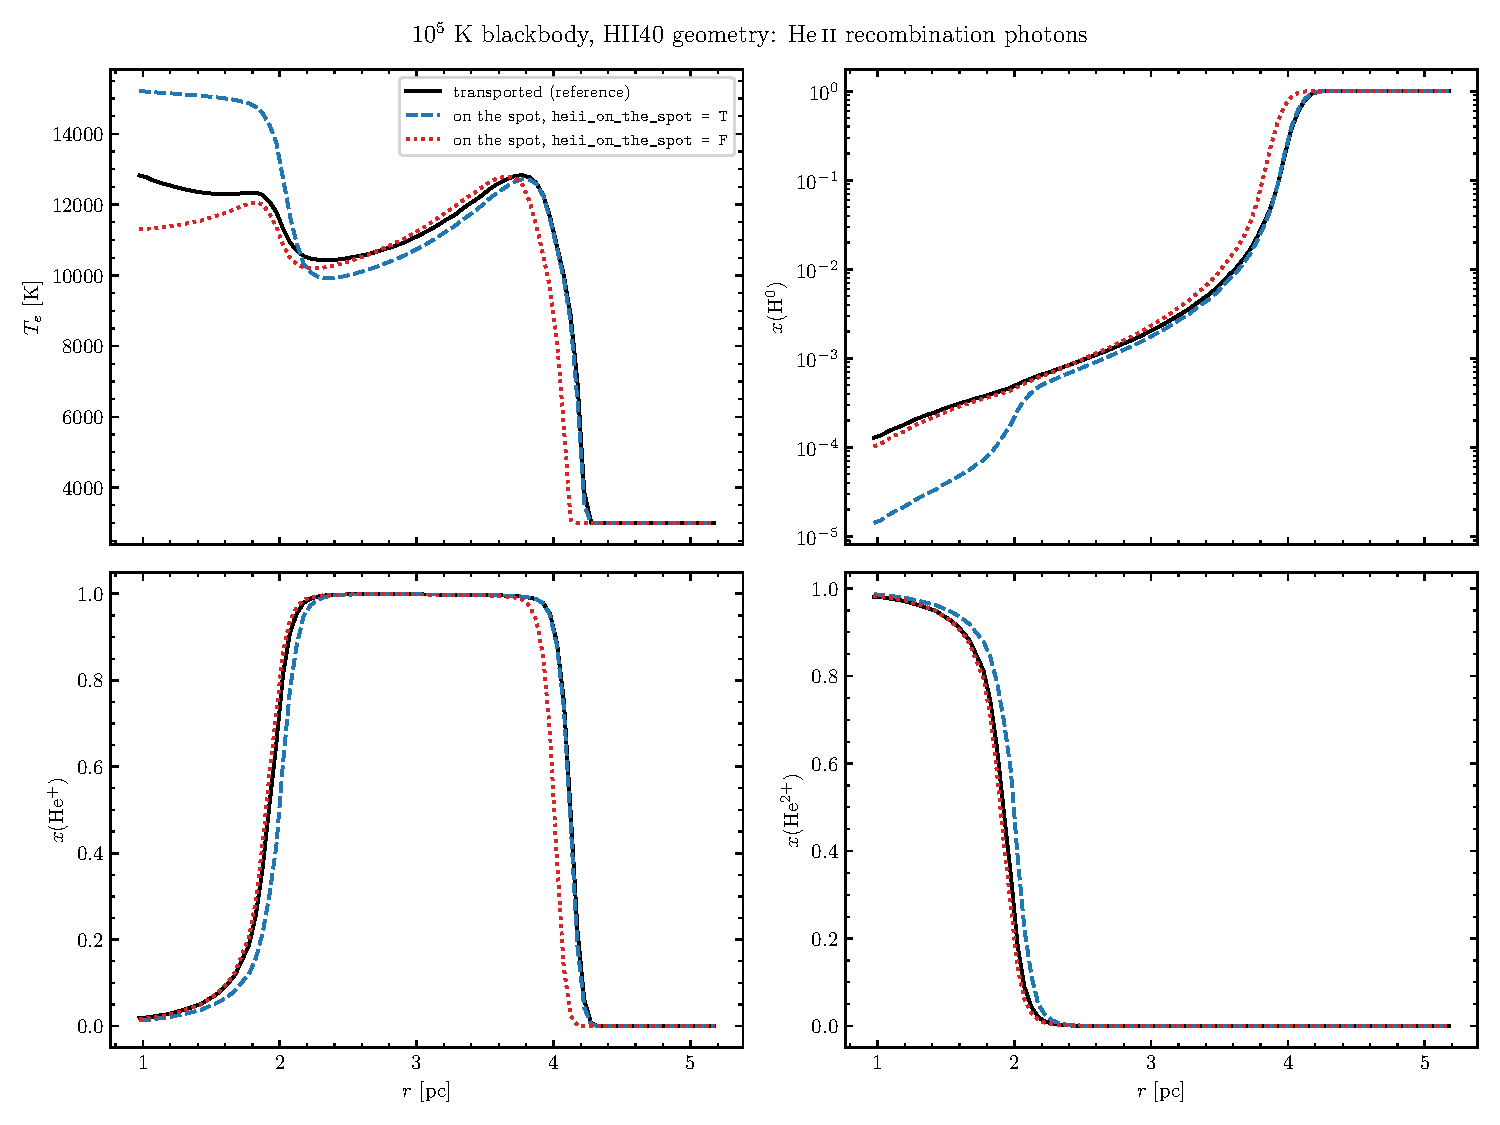
\includegraphics[width=0.95\textwidth]{../results/heii_on_the_spot/heii_ots_profiles.pdf}
\caption{Spherically averaged $T_e$, $x({\rm H^0})$, $x({\rm He^+})$ and
$x({\rm He^{2+}})$ of the three runs of Section~\ref{sec:ots-heii}
(\code{results/heii\_on\_the\_spot/plot\_profiles.py}).}
\label{fig:heii-ots}
\end{figure}

\subsection{Explicit diffuse LyC field and packet sampling}
\label{sec:diffuse}
With \code{par\%recombination\_continuum = 'transported'} (the default
since 2026-09-26) case B on the spot is replaced by case A rates plus
explicit emission of recombination packets.  For each leaf and each of the
three ground continua H\,\textsc{ii}$\rightarrow$H\,\textsc{i}($1s$),
He\,\textsc{ii}$\rightarrow$He\,\textsc{i}($1^1S$), and
He\,\textsc{iii}$\rightarrow$He\,\textsc{ii}($1s$), the emissivity uses
the Milne $\alpha_1(T)$ of Eq.~(\ref{eq:milne-alpha1}), which is
$\alpha_A(T)-\alpha_B(T)$ by construction (\S\ref{sec:hherec}); channels
4 and 5 carry the He\,\textsc{i} and He\,\textsc{iii} excited cascades,
and, since 2026-10-11, channel 6 the metal ground continua and channel 7
the free--free emission inside the band; channel 8, off by default, the
\textsc{Cloudy} valence-fraction photons kept for comparison (all below).  At the start of every gas
iteration the code rebuilds the energy-luminosity table
\begin{equation}
 L_{{\rm ch},l} = n_{e,l}n_{{\rm rec},l}\alpha_{1,\rm ch}(T_l)
      \left<E\right>_{n,\rm ch}(T_l)\,V_l,
 \qquad L_{\rm dif}=\sum_{l,{\rm ch}} L_{{\rm ch},l},
 \label{eq:diffuse-luminosity}
\end{equation}
with $\left<E\right>_n$ the photon-number-weighted mean energy of the
emitted continuum.

\paragraph{Ground-continuum spectrum (\code{par\%diffuse\_energy\_model}).}
Detailed balance between photoionization and radiative recombination fixes
the free--bound spectrum.  Per unit photon energy the photon-number
emissivity of each ground continuum is
\begin{equation}
 n(E)\;\propto\;E^2\,\sigma_{\rm pi}(E)\,
   \exp\!\left[-\frac{E-E_{\rm th}}{kT_e}\right],
 \qquad E\ge E_{\rm th},
 \label{eq:milne-pdf}
\end{equation}
evaluated with the \emph{same} ground-state cross section the transport
absorbs with, so a packet is absorbed with the cross section it was emitted
with.  This is the default, \code{'milne'}.  Restoring the Milne prefactor
turns the same integral into the ground-state recombination coefficient,
\begin{equation}
 \alpha_1(T)=\frac{g_n}{2g_+}\,\frac{2}{\sqrt{\pi}}\,(kT)^{-3/2}
   \sqrt{\frac{2}{m_e}}\,\frac{1}{m_ec^2}
   \int_{E_{\rm th}}^{\infty}\!E^2\sigma_{\rm pi}(E)
   e^{-(E-E_{\rm th})/kT}\,dE ,
 \label{eq:milne-alpha1}
\end{equation}
so the spectrum and the emission rate are not independent assumptions.
Equation~(\ref{eq:milne-alpha1}) reproduces
$\alpha_{1s}({\rm H\,\textsc{i}},10^4~{\rm K})=1.579\times10^{-13}$
cm$^3$\,s$^{-1}$ against the tabulated $1.58\times10^{-13}$.  The code
reports that integral at start-up against the $\alpha_A-\alpha_B$ that sets
the packet count and rescales neither side.  Since the correction described
next, the largest disagreement over the three channels is $0.01\%$.  It was
$3.44\%$ before, all of it in He\,\textsc{i}, and that number is what
exposed the defect.

\paragraph{The $\alpha_1$ source-mixing defect.}  \code{recomb\_mod} took
$\alpha_A$ from the Badnell total, $\alpha_1$ from the \emph{level-resolved}
Mao \& Kaastra fit, and then defined $\alpha_B = \alpha_A - \alpha_1$.  That
subtraction crosses two unrelated determinations.  Nothing in the
construction forces the Mao $n{=}1$ value to be the ground term of the
Badnell total it is subtracted from, and whatever separates them lands
entirely in $\alpha_B$ --- and, through $\alpha_1$, in the diffuse packet
count as well.

The cross-section side is not the error.  MoCHII's \code{sigma\_HeI}
reproduces Verner's own \code{phfit2.f} to a ratio of $1.00000$ at every
energy over $24.6$--$105$~eV, and its threshold value, $7.436$~Mb, sits
$0.5\%$ above the measured $7.40\pm0.07$~Mb of Samson et al.\ (1994),
inside the experimental uncertainty.  Nor is the start-up comparison between
unlike quantities: because $\alpha_B = \alpha_A - \alpha_1$, the ``rates''
side of it \emph{is} $\alpha_1$(He\,\textsc{i}) itself, so the $3.44\%$
separated two determinations of one number.

\paragraph{Cloudy settles which side is right.}  Cloudy c25.00 derives its
H-like and He-like recombination level by level from its \emph{own}
photoionization cross sections through the exact Milne relation
(\code{source/iso\_radiative\_recomb.cpp}), caching the result in
\code{data/h\_iso\_recomb.dat} and \code{data/he\_iso\_recomb.dat}.  In those
files row 0 of each element is the ground level and the last row is the
total --- verified on hydrogen, where row 0 is $1.5840{\times}10^{-13}$ and
the last row $4.1642{\times}10^{-13}$ against the known
$\alpha_{1s} = 1.58{\times}10^{-13}$ and
$\alpha_A = 4.18{\times}10^{-13}\,\cmc$.  At $10^4$~K, in
$10^{-13}\,\cmc$:
\begin{center}\small
\begin{tabular}{@{}lrrrrr@{}}
\toprule
& \multicolumn{2}{c}{$\alpha_A$} & \multicolumn{3}{c}{$\alpha_1$} \\
\cmidrule(r){2-3}\cmidrule(l){4-6}
channel & MoCHII & Cloudy & Mao \& Kaastra & Milne integral & Cloudy \\
\midrule
H\,\textsc{i}   & 4.1933 & 4.1642 & 1.5873          & 1.5790 & 1.5840 \\
He\,\textsc{i}  & 4.3719 & 4.3583 & \textbf{1.5650} & 1.6086 & 1.6032 \\
He\,\textsc{ii} & 21.895 & 21.817 & 6.5366          & 6.5116 & 6.5145 \\
\bottomrule
\end{tabular}
\end{center}
(The MoCHII $\alpha_A$ column is the Badnell total all three channels used
then; since 2026-09-26 H\,\textsc{ii} and He\,\textsc{iii} take $\alpha_B$
from the Storey \& Hummer cascade, which gives $\alpha_A = 4.1624$ and
$21.821$, $-0.04\%$ and $+0.02\%$ from Cloudy.)
Badnell's totals are accurate to $0.3$--$0.7\%$ on all three channels, and
the Mao $n{=}1$ values to $0.2$--$0.3\%$ for H\,\textsc{i} and
He\,\textsc{ii} --- but He\,\textsc{i} is $2.38\%$ low, and the subtraction
propagates that into $\alpha_B$(He\,\textsc{i}) as $+1.88\%$.  MoCHII's own
Milne integral matches Cloudy to $0.3\%$, $0.34\%$ and $0.04\%$.  The Milne
relation is exact, Cloudy applies it to a He$^0$ ground cross section that
agrees with Verner's to the $0.4\%$ implied by the $\alpha_1$ agreement, and
so \emph{the Milne route is the correct one and the level-resolved fit is
the low side}.

\paragraph{An earlier reading of the same numbers, withdrawn.}  This
document previously concluded the opposite --- that the Milne integral was
the outlier --- from the third determination available at the time,
Benjamin, Skillman \& Smits (1999) with J.~S.\ Mathis as carried by
K.~Wood's \code{ionize},
$\alpha_1({\rm He\,\textsc{i}}) = 1.54{\times}10^{-13}(T_4)^{-0.486}$
$\cmc$:
\begin{center}\small
\begin{tabular}{lrrrr}
\toprule
$T$ & BSS99 $+$ JSM & Mao \& Kaastra & Milne integral & Cloudy c25.00 \\
\midrule
$5000$~K       & 2.157 & 2.184 ($+1.3\%$) & 2.259 ($+4.8\%$) & --- \\
$10^4$~K       & 1.540 & 1.565 ($+1.6\%$) & 1.609 ($+4.5\%$) & 1.603 ($+4.1\%$) \\
$2{\times}10^4$~K & 1.100 & 1.128 ($+2.6\%$) & 1.151 ($+4.7\%$) & --- \\
\bottomrule
\end{tabular}
\end{center}
In $10^{-13}\,\cmc$, percentages against the BSS99 column.  The arithmetic
was right --- the Milne integral does sit $4.5$--$4.8\%$ above BSS99 and
$2.8\%$ above Mao while the two fits cluster within $2.6\%$ of each other
--- but the inference was a majority vote taken on the mutual closeness of
two fits, which is not evidence that either reproduces the cross sections in
use.  Cloudy, computing the same quantity level by level from its own cross
sections, lands within $0.34\%$ of the Milne integral.  The earlier
conclusion is withdrawn.

\paragraph{The correction.}  \code{tools/fitting/fit\_alpha1\_milne.py}
evaluates Eq.~(\ref{eq:milne-alpha1}) on the cross sections the transport
actually uses --- exact hydrogenic for H\,\textsc{i} and He\,\textsc{ii}
(\code{sigma\_hydrogenic}, $Z = 1$ and 2; note that \code{sigma\_HI} in
\code{src/photo\_xsec.f90} is the exact hydrogenic form, not VFKY96) and
VFKY96 for He\,\textsc{i} --- at 241 temperatures over $10^3$--$10^5$~K, and
refits the same seven coefficients of Eq.~(\ref{eq:mao}), so that no Fortran
structure changes:
\begin{center}\small
\begin{tabular}{@{}lp{112mm}@{}}
\toprule
function & $(a_0,\,b_0,\,c_0,\,a_1,\,b_1,\,a_2,\,b_2)$ \\
\midrule
\code{alpha1\_HII}   & $1.87007{\times}10^{-2}$, $1.29077$,
  $-2.17465{\times}10^{-3}$, $1.29189{\times}10^{1}$,
  $8.05060{\times}10^{-1}$, $8.44399{\times}10^{-2}$,
  $5.93940{\times}10^{-4}$ \\
\code{alpha1\_HeII}  & $3.26862{\times}10^{-3}$, $6.97361{\times}10^{-1}$,
  $3.14907{\times}10^{-4}$, $5.76341{\times}10^{1}$, $1.18534$,
  $2.58417{\times}10^{1}$, $9.90134{\times}10^{-1}$ \\
\code{alpha1\_HeIII} & $2.61525{\times}10^{-1}$, $1.39527$,
  $-3.22079{\times}10^{-4}$, $6.40708{\times}10^{1}$,
  $8.97582{\times}10^{-1}$, $5.01551{\times}10^{-1}$,
  $1.21533{\times}10^{-3}$ \\
\bottomrule
\end{tabular}
\end{center}
The largest $|{\rm fit}/{\rm Milne}-1|$ is $0.019\%$ (H\,\textsc{i}),
$0.001\%$ (He\,\textsc{i}) and $0.006\%$ (He\,\textsc{ii}) over
$10^3$--$10^5$~K, and $0.0075\%$, $0.0004\%$, $0.0021\%$ over the production
range $3{\times}10^3$--$3{\times}10^4$~K, so the functional form is not the
limiting approximation.  At $10^4$~K the fitted $\alpha_1$ is $1.5791$,
$1.6086$ and $6.5117{\times}10^{-13}\,\cmc$: within $0.35\%$ of Cloudy on
all three channels, with He\,\textsc{i} corrected from $-2.38\%$ to
$+0.34\%$.  The code's own cross-check confirms it, \code{milne\_setup}
reporting a largest $\alpha_1$ disagreement of $3.44\%$ before and $0.01\%$
after.

The gate is \code{tests/milne/check\_alpha1.f90}, wired into
\code{tests/milne/run\_check.sh}.  It re-implements the Milne quadrature
independently from \code{photo\_xsec}, checks the three channels at 81
temperatures over $10^3$--$10^5$~K to $10^{-3}$, checks
$\alpha_1 < \alpha_A$ everywhere (largest $\alpha_1/\alpha_A$ $0.560$,
$0.496$, $0.445$), and checks all three against the hardcoded Cloudy c25.00
values to $1\%$.  Reinstating the old Mao He\,\textsc{i} coefficients makes
it fail on both counts ($3.886{\times}10^{-2}$ from the quadrature, $2.383\%$
from Cloudy) and it passes again after reverting.

\paragraph{Effect on the benchmarks, graded against the prediction.}  What
was recorded before the runs: ``$\alpha_1$(He\,\textsc{i}) rises $2.4\%$, so
channel 2 emits more; $\alpha_B$(He\,\textsc{i}) falls $1.9\%$, so there is
less case-B recombination.  Both push the front outward, toward Cloudy, by
of order $0.015$--$0.02$~pc.''  Measured on the paired HII40/HII20
production runs (68 ranks, same Sobol seed, converged in 38 and 27
iterations as before):
\begin{center}\small
\begin{tabular}{@{}lrr@{}}
\toprule
 & HII40 & HII20 \\
\midrule
$\Delta r({\rm He^0}{=}0.5)$ & $+0.00811$~pc & $+0.00210$~pc \\
Cloudy residual & $-0.18561 \to -0.17750$~pc & --- \\
$\Delta L({\rm H}\beta)$ & $-0.3713\%$ & $-0.4159\%$ \\
mean $T_e(\xHI < 0.95)$ & $9053.4 \to 9051.7$~K & $8522.3 \to 8528.7$~K \\
\bottomrule
\end{tabular}
\end{center}
The \emph{sign} was right, outward and toward Cloudy on both benchmarks.
The \emph{magnitude} was about half the low end of the predicted range,
$+0.0081$ against $0.015$--$0.02$~pc, so the prediction was roughly a factor
two high.  \code{tests/continuous\_energy/check\_hii\_production.py} passes
on both, with energy closure $1.5{\times}10^{-16}$ and $0$.  The published
benchmark quantities move by less than the width of the published spread:
$\langle T[N_pN_e]\rangle$ from 8162 to 8169~K at HII40 and 6917 to 6925~K
at HII20, $T_{\rm inner}$ from 7535 to 7536 and 6936 to 6938~K, and $R_{\rm
out}$ from $8.89$ to $8.88{\times}10^{18}$~cm at HII20 with
$1.44{\times}10^{19}$~cm unchanged at HII40.  A later, independent
correction --- exchanging the oxygen charge-exchange rows of
\S\ref{sec:cx} --- then carries these a further $+2.2$~K at HII40 and
$+2.1$~K at HII20, to 8170 and 6926~K (8177 and 6936~K after the 2026-09-24
update, all early-stopped; the current values are in \S\ref{sec:hii}).

$L({\rm H}\beta)$ moves the \emph{wrong} way.  It falls $0.37$--$0.42\%$
($1.94 \to 1.93{\times}10^{37}$ and $4.70 \to 4.68{\times}10^{36}\,{\rm
erg\,s^{-1}}$), taking MoCHII from about $3\%$ below the published
$2.01$--$2.10{\times}10^{37}$ at HII40 to slightly further below.  The
likely route is channel 1: $\alpha_1$(H\,\textsc{i}) drops $0.52\%$ from the
Mao value to the Milne one, so the H\,\textsc{i} ground continuum recycles
marginally fewer H-ionizing photons.  This is not an argument against the
change --- the acceptance criterion is physical correctness, and an exact
relation was being violated --- but it is recorded rather than buried.

Two legacy options remain.  \code{'exponential'} is the historical
near-threshold approximation
\begin{equation}
 E_{\rm pkt}=E_{\rm th}+kT_e[-\ln(\max(u,\epsilon))],
 \label{eq:diffuse-energy}
\end{equation}
i.e.\ Eq.~(\ref{eq:milne-pdf}) with the $E^2\sigma_{\rm pi}$ weight dropped;
it is kept to reproduce earlier runs.  \code{'threshold'} emits at
$E_{\rm th}$ and is a sensitivity bracket, not a model.  The three
thresholds are 13.598, 24.587, and 54.416~eV, and every model is a sampled
photon energy, not a bin-center approximation.

\paragraph{Sampling weight.}  MoCHII emits equal-energy packets and fixes
their number from the channel's \emph{energy} luminosity.  The packet
energies must therefore follow the energy-luminosity density $E\,n(E)$,
not $n(E)$ itself.  With that pairing the represented photon rate is exactly
the physical one,
\begin{equation}
 N_{\rm pkt}L_{\rm pkt}\left<E^{-1}\right>_{En}
   = R\left<E\right>_n\frac{1}{\left<E\right>_n}=R ,
\end{equation}
whereas drawing from $n(E)$ while counting packets from the energy
luminosity inflates it by $\left<E\right>_n\left<E^{-1}\right>_n>1$
(1.002 at $8000$~K, 1.010 at $2\times10^4$~K).  The CDF is tabulated in
$x=(E-E_{\rm th})/kT$, interpolated in $\log T$ and inverted once, rather
than inverting two neighboring temperature rows and interpolating the
resulting energies.

\paragraph{Effect.}  Against the exponential approximation the converged
HII40 calculation moves $r({\rm He^0}=0.5)$ outward by $0.00063$~pc and
$r({\rm C^{2+}}=0.5)$ by $0.00052$~pc, closing $0.3\%$ of the residual
against Cloudy c25.  The two continua move in opposite directions because
each follows its own mean energy: the H\,\textsc{i} continuum softens
($14.460\rightarrow14.427$~eV at $10^4$~K) since the hydrogenic cross
section falls as $E^{-3}$, while the He\,\textsc{i} continuum hardens
($25.449\rightarrow25.460$~eV) because the Verner He\,\textsc{i} fit falls
more slowly near threshold.  The exact spectrum is therefore a correctness
fix, not the explanation of the Cloudy front residual.  The same holds for
the three He\,\textsc{i} cascade corrections described below: the two-photon
shape moves $r({\rm He^0}=0.5)$ by $-0.00030$~pc, the branch fractions by
$+0.00024$~pc, and the fate of the 584~\AA{} photon by $-0.00363$~pc.  All
four corrections to the emitted diffuse spectrum together move it
$-0.00306$~pc, i.e.\ $1.7\%$ of the $0.18$~pc residual and \emph{away} from
Cloudy rather than toward it.  Switching the whole fourth channel off moves
it $-0.103$~pc, so the channel's presence matters and its internal detail
does not.

\emph{Record (2026-09-25).}  The front shifts and bounds in this part were
measured on runs stopped by the earlier convergence rule (\S\ref{sec:hii}),
which ended the HII40 benchmark 0.17~pc short of its converged He\,\textsc{i}
front; they document the search for a residual that was mostly that early
stop, and are not current bounds.  The converged residual is $0.025$~pc
(\code{m13\_restoration}, $4.2803$ against $4.3053$~pc; $0.033$~pc in
\code{m11\_hecx\_solver}).

\paragraph{Where the Cloudy front residual is not.}  Each of those four
corrections is independently correct --- three of them reproduce an external
reference implementation and the first an exact detailed-balance relation ---
and the acceptance criterion is physical correctness, not agreement with a
particular reference calculation, so a net displacement in the unhelpful
direction is not an argument against any of them.  What the sum does settle
is the diagnosis: \emph{the $0.18$~pc residual is not in what the diffuse
field emits.}  Four independent corrections, spanning the emitted spectrum's
shape, its branch weights and the fate of its strongest line, together
account for $1.7\%$ of the gap and with the wrong sign.

\paragraph{Bounding the remaining candidates.}  The quantity to be explained
is $r({\rm He^0}=0.5) = 4.12781$~pc against Cloudy c25.00's $4.30531$~pc,
i.e.\ $-0.17750$~pc after the $\alpha_1$ correction above.  The sensitivity
runs below were measured against the pre-correction production point,
$4.11970$~pc; the $0.008$~pc between the two baselines changes no lever, and
the raw front positions are quoted as measured.  The front's sensitivity to
the diffuse field is
calibrated two ways from the 584~\AA{} measurement above: differentially
(channel 4 lost $8.87\%$ of its energy, is $17.6\%$ of the diffuse field, and
moved the front $0.00363$~pc) and by switching that channel off entirely
($17.6\%$ of the field, $0.103$~pc), giving $0.233$ and $0.585$~pc per unit
fractional change in the total diffuse band luminosity.  Two further
sensitivity runs (HII40, 68 ranks, same Sobol stream, 38 iterations) scale
the He\,\textsc{i} atomic data by $3\%$: reducing
$\sigma_{\rm pi}$(He\,\textsc{i})
moves the front $+0.00799$~pc and reducing the He\,\textsc{i} recombination
rate moves it $+0.02410$~pc.  Every candidate then has a number attached to
it, and every number is too small:
\begin{center}\small
\begin{tabular}{@{}lll@{}}
\toprule
axis & bound measured & to reach $0.178$~pc \\
\midrule
what the diffuse field emits & four corrections, net $-0.00306$~pc
  & wrong sign \\
explicit transport vs.\ on-the-spot$^\dagger$ & 4.11970 to 4.18159~pc
  & the whole range is $0.062$~pc \\
total diffuse band luminosity & $0.233$--$0.585$~pc per unit fraction
  & $30$--$76\%$ \\
$\sigma_{\rm pi}$(He\,\textsc{i}) & $+0.00799$~pc per $-3\%$ ($0.27$~pc/unit)
  & ${\sim}70\%$ \\
$\alpha$(He\,\textsc{i}) & $+0.02410$~pc per $-3\%$ ($0.80$~pc/unit)
  & ${\sim}23\%$ \\
$\alpha_A$, $\alpha_1$, $\alpha_B$(He\,\textsc{i})
  & $0.3\%$, $0.34\%$, $1.9\%$ from Cloudy (\S\ref{sec:henetwork})
  & already there; code spread is $11\%$ \\
metal opacity & $0.103$~pc/unit upward, $0.615$ downward
  (\S\ref{sec:metalop}) & $+180\%$, and saturating \\
metal recombination continua & $0.29\%$ of channel 2 & ${\sim}0.001$~pc \\
He\,\textsc{i} excited-level ionization & $0.2$--$0.6\%$ extra, and below the
  band floor & structurally absent \\
dust & \code{dust\_density\_law='none'} in the benchmark & excluded by construction \\
source photon budget & $Q$ ratios $1.00005$ and $1.00003$ & $14\%$ in
  $Q({\rm He^0})$ \\
Cloudy-side resolution & median zone width $0.0106$~pc at the front
  & $17\times$ finer already \\
\bottomrule
\end{tabular}

\smallskip
{\footnotesize $^\dagger$ Measured before the on-the-spot He\,\textsc{i}
photons of Section~\ref{sec:ots-hei} existed: the on-the-spot end then gave
every He recombination photon back to helium.}
\end{center}
The transport entry is the decisive one, because it was the leading candidate:
switching the whole diffuse treatment between its extremes --- explicit
transport at $4.11970$~pc and the on-the-spot approximation at $4.18159$~pc
--- spans only $0.062$~pc, and Cloudy sits $0.124$~pc beyond the more
favorable end of that range.  No choice about how diffuse photons are
transported can reach it.  The photon budget is verified against the same
40-kK blackbody Cloudy was given: $Q({>}13.598~{\rm eV}) =
4.2656{\times}10^{49}$~s$^{-1}$ against $4.2653{\times}10^{49}$ and
$Q({>}24.587~{\rm eV}) = 4.6082{\times}10^{48}$ against
$4.6081{\times}10^{48}$, ratios $1.00005$ and $1.00003$.  Cloudy resolves the
front with 40 zones between 4.0 and 4.6~pc, median width $0.0106$~pc and
maximum $0.039$~pc, so the reference position is not a resolution artifact
either.

\paragraph{The He-ionizing photon budget.}  Where the sensitivity lives is
visible in the budget itself.  Integrated over the He$^+$ zone of the
converged HII40 model:
\begin{center}\small
\begin{tabular}{@{}lr@{}}
\toprule
HII40 & s$^{-1}$ \\
\midrule
stellar $Q({>}24.587$~eV) & $4.6082{\times}10^{48}$ \\
diffuse He\,\textsc{i} ground continuum, recycled & $1.6135{\times}10^{48}$ \\
total He-ionizing supply & $6.2217{\times}10^{48}$ \\
He$^0$ photoionizations $=$ case-A recombinations & $4.7008{\times}10^{48}$ \\
absorbed by H$^0$ or metals, or escaped
  & $1.5210{\times}10^{48} = 24.4\%$ of the supply \\
\bottomrule
\end{tabular}
\end{center}
Nearly a quarter of the He-ionizing supply is lost to absorbers other than
He$^0$, and halving that loss fraction alone would move the front
$0.211$~pc.  The H$^0$/He$^0$ competition is therefore the one place where a
few-percent difference has the leverage to matter, which is consistent with
the radial signature below and with the metal-opacity mechanism of
\S\ref{sec:metalop}.  The budget also closes geometrically: with the leaf
volume computed correctly the summed gas volume matches the geometric shell
$0.972$--$4.729$~pc to $0.25\%$.  (\code{LeafSize} in the output is the leaf
\emph{full} width, and the residual analysis script had used
$(2\,\mathrm{size})^3$, eight times the cell volume.  Because it enters only
as a relative weight within a shell, every front position reported from it is
unaffected and re-running after the fix reproduces all of them identically;
the expression was nevertheless wrong and is now $\mathrm{size}^3$.  The
table generator, the Python readers and the g1/g4 gates all used the
convention correctly and were never affected.)

\paragraph{The radial signature.}  What the residual does have is a shape.
The hydrogen structure agrees with Cloudy throughout the ionized zone; only
the helium structure drifts, and it drifts monotonically outward:
\begin{center}
\begin{tabular}{lrrrrrr}
\toprule
$r$ [pc] & 1.6 & 2.0 & 2.5 & 3.0 & 3.5 & 3.8 \\
\midrule
$x({\rm He^0})$, MoCHII/Cloudy & 1.007 & 1.015 & 1.031 & 1.059 & 1.109
  & 1.196 \\
$x({\rm H^0})$, MoCHII/Cloudy  & 0.981 & 0.984 & 0.989 & 1.000 & 1.005
  & 1.009 \\
\bottomrule
\end{tabular}
\end{center}
A normalization difference in a rate or a cross section would be
radius-independent; this one compounds with depth.  That is what a $0.7\%$
seed at 1.6~pc must do when He$^0$ carries almost all of the opacity above
24.6~eV: at 30~eV,
$\kappa({\rm He^0})/[\kappa({\rm He^0})+\kappa({\rm H^0})]$ rises from
$0.843$ at 1.6~pc to $0.956$ at 4.0~pc, so any excess He$^0$ shortens the
mean free path of the very photons that would have removed it.  The
signature therefore identifies a small helium-specific seed, amplified
geometrically, rather than a large error anywhere.

Closing $0.178$~pc is $4.1\%$ in radius and $13\%$ in volume, which asks for
$Q({\rm He^0})$ higher by ${\sim}14\%$ or $\alpha_B$(He\,\textsc{i}) lower by
${\sim}20\%$.  $Q({\rm He^0})$ is verified to $0.003\%$, and MoCHII's
$\alpha_A$, $\alpha_1$ and $\alpha_B$(He\,\textsc{i}) now sit within $0.3\%$,
$0.34\%$ and $1.9\%$ of Cloudy's own level-resolved values, with no
published determination anywhere near $20\%$ away.  \emph{The residual is
therefore unexplained}, and what has been achieved is the systematic closing
of the space of simple explanations: it is not in what the diffuse field
emits, not in how those photons are transported, not in the He\,\textsc{i}
photoionization cross section, not in the He\,\textsc{i} recombination rate,
not in the metal opacity, not in the metal recombination continua, not in
He\,\textsc{i} excited-level ionization, not in dust, not in the source
photon budget, and not in the reference calculation's resolution.

The two candidates named in earlier revisions have both been examined and
neither survives as a single parameter.  The helium ionization
\emph{network} has been compared code to code (\S\ref{sec:henetwork}): every
code sums the full cascade, MoCHII's $\alpha_A$(He\,\textsc{i}) agrees with
Cloudy's explicit level sum to $0.3\%$, and the He\,\textsc{i} excited levels
that a resolved model atom carries are worth $0.2$--$0.6\%$ of extra
ionization.  The metal opacity has been measured
(\S\ref{sec:metalop}): its upward derivative is $0.103$~pc per unit, so
closing the gap would need $+180\%$ against cross sections that reproduce
Verner's to $10^{-6}$ and an Opacity Project comparison that runs $2$--$14\%$
the other way.

What remains is the one hypothesis that no single-parameter experiment can
reproduce: several differences of a few percent each --- in the He\,\textsc{i}
recombination rate, in the shape of $\sigma_{\rm pi}$(He\,\textsc{i}), in the
metal opacity of the $21$--$40$~eV window, in Cloudy-side modeling choices
not yet identified --- acting together through the He$^0$ optical depth,
which compounds them with depth exactly as the radial signature shows.  Each
is individually below its own measured lever; their product over $24.4\%$ of
the He-ionizing supply lost to competing absorbers is not bounded by any of
the experiments above.  Testing it requires varying several ingredients
jointly, not one at a time, and that is the open item.

The number of diffuse packets is $N_{\rm dif} = \max[1,
\mathrm{nint}(L_{\rm dif}/L_{\rm pkt})]$, with $L_{\rm pkt}$ the luminosity
of one ionizing source packet ($L_{\rm ion}/N$; with the FUV extension the
ionizing stratum's), and each carries $L_{\rm dif}/N_{\rm dif}$, so the
emitted luminosity is exactly $L_{\rm dif}$ (until 2026-09-25 each carried
$L_{\rm pkt}$, off by up to half a packet, and a field under half a packet
was dropped).  A packet first selects a leaf from the CDF of
$\sum_{\rm ch}L_{{\rm ch},l}$, then a channel from that leaf's luminosity
weights over the seven channels.  Its emission point is
uniform in the selected cubic leaf and its direction is isotropic.  It is
then transported with the same exact-energy edge walk and path estimator as
a stellar packet.  Hence diffuse luminosity is represented by packet count,
each packet carrying the stellar packet luminosity to within a factor
$1 \pm 1/(2N_{\rm dif})$.  At HII40 the diffuse band luminosity
converges to $7.28{\times}10^{38}$~erg/s $=0.57\,L_\star$ in the current
run (\code{m13\_restoration}; $7.25{\times}10^{38}$ in \code{m11\_hecx\_solver},
$1.9{\times}10^7$ diffuse packets an iteration; earlier revisions recorded
$6.8{\times}10^{38}$~erg/s).

For output bookkeeping, the sampled energy is
mapped by binary search of \code{ion\_eedge} (\code{ion\_bin\_of}).  This
works for both threshold-aligned and logarithmic diagnostic grids; an energy
on an edge falls in the bin above it.  The assignment is a tally address
only: it does not modify $E_{\rm pkt}$ or its cross sections.  The
binary search also corrects the former closed-form log-grid mapping, which
could place a 24.6-eV He\,\textsc{i} recombination photon below the
He\,\textsc{i} threshold on an aligned grid.

\paragraph{He\,\textsc{i} excited-level recombination
(\code{par\%hei\_diffuse}).}
A fourth channel adds the He\,\textsc{i} \emph{excited-level} recombination
radiation (previously those photons simply vanished).  Every case-B
He\,\textsc{ii} recombination reaches $1^1{\rm S}$ through exactly one
$n = 2$ term, so what the channel needs is not three absolute rates but
three \emph{branch fractions}; the absolute rate is already fixed by the
$\alpha_B({\rm He\,II})$ that sets the packet count.  MoCHII takes all three
from one internally consistent set of effective recombination coefficients,
\begin{equation}
\begin{aligned}
 \alpha_{\rm eff}(2^3{\rm S}) &= 2.10{\times}10^{-13}\,(T_4)^{-0.381}, \\
 \alpha_{\rm eff}(2^1{\rm S}) &= 2.06{\times}10^{-14}\,(T_4)^{-0.451}, \\
 \alpha_{\rm eff}(2^1{\rm P}) &= 4.17{\times}10^{-14}\,(T_4)^{-0.695},
\end{aligned}
 \label{eq:hei-branch}
\end{equation}
in $\cmc$ --- Benjamin, Skillman \& Smits (1999) Table~1 with J.~S.\ Mathis,
in the form carried by K.~Wood's \code{ionize} --- and normalizes by their
sum.  That all three come from one source matters more than any individual
value: a fraction assembled from fits with unrelated temperature dependences
is not a fraction of anything.  Normalizing by the sum is the source's own
choice, made for the reason it states, that the fitting formulae carry
different temperature dependences.  Outside $3{\times}10^3$--$2{\times}10^4$~K
the fits are clamped, not extrapolated.

The closure
\begin{equation}
 \alpha_{\rm eff}(2^3{\rm S}) + \alpha_{\rm eff}(2^1{\rm S})
   + \alpha_{\rm eff}(2^1{\rm P}) = \alpha_B({\rm He\,II})
 \label{eq:hei-closure}
\end{equation}
is physically true, but MoCHII does \emph{not} use it to derive a branch.
Its two sides are independent atomic data: the three fits of
Eq.~(\ref{eq:hei-branch}) account for $0.90\,\alpha_B$ at 8000~K and
$0.97\,\alpha_B$ at $10^4$~K, and the ratio is reported at start-up rather
than absorbed.  Forcing it onto $\alpha_B$ would dump the entire mismatch
between two data sets into whichever branch was solved for last.  The
resulting fractions, as the code prints them, are
\begin{center}
\begin{tabular}{lcccc}
\toprule
$T$ [K] & $2^3$S & $2^1$S & $2^1$P & $\sum\alpha_{\rm eff}/\alpha_B$ \\
\midrule
$5{\times}10^3$   & 0.74084 & 0.07629 & 0.18288 & 0.767 \\
$8{\times}10^3$   & 0.76183 & 0.07591 & 0.16226 & 0.896 \\
$10^4$            & 0.77121 & 0.07565 & 0.15314 & 0.970 \\
$1.5{\times}10^4$ & 0.78729 & 0.07507 & 0.13764 & 1.134 \\
\midrule
statistical & 0.75000 & 0.08333 & 0.16667 & --- \\
\bottomrule
\end{tabular}
\end{center}
against the AGN3 low-density statistical weights of the last row, which the
code used before.  The correction is a moderate temperature-dependent shift,
not a reordering.

Two provenance points belong with these numbers.  First,
$2.06{\times}10^{-14} + 4.17{\times}10^{-14} = 6.23{\times}10^{-14}$
exactly, so the $6.23{\times}10^{-14}(T_4)^{-0.827}$ that \code{nebcont\_mod}
took from MOCASSIN for the He\,\textsc{i} two-photon continuum
(Section~\ref{sec:twophoton}) is the \emph{singlet total}, not
$\alpha_{\rm eff}(2^1{\rm S})$.  An earlier version of this section read it
as the latter and closed $2^1$P against $\alpha_B$, obtaining
$0.746 : 0.224 : 0.031$ together with an argument that case-B trapping
inverts the singlet split; both the numbers and the argument are withdrawn.
Second, the 2$^3$S population of \code{hei\_metastable\_mod}
(Section~\ref{sec:heimeta}) takes its recombination source from this set:
$\alpha_3 = f_{3S}\,\alpha_B({\rm He\,II})$.  It used to carry its own
Oklopcic \& Hirata (2018) fit, $2.10{\times}10^{-13}(T_4)^{-0.778}$, which an
earlier version of this paragraph defended as a separate ``absolute
production rate''.  That defense is withdrawn (2026-09-25): the absolute rate
of triplet recombinations is fixed once the balance's $\alpha_B$ and the
branch fraction are, and a second normalization supplied beside them is the
defect of lesson~(4).

The $2^1$S photons follow the tabulated Drake, Victor \& Dalgarno (1969)
distribution (\code{data/HeI2phot.dat}, the same table the nebular continuum
uses) rather than a flat draw.  That shape fixes the H-ionizing yield at
0.55644 photons and 8.9646~eV per decay, with a mean in-band energy of
16.110~eV, against the 0.56 and 17.109~eV of the flat surrogate.  The two
corrections are individually small and act in opposite directions.  Per
case-B He\,\textsc{ii} recombination the channel emits
\begin{center}
\begin{tabular}{lcc}
\toprule
 & H-ionizing energy [eV] & photons \\
\midrule
statistical weights, flat two-photon & 19.200 & 0.9634 \\
statistical weights, Drake shape     & 19.149 & 0.9633 \\
Eq.~(\ref{eq:hei-branch}), Drake shape, 8000~K & 19.223 & 0.9663 \\
\bottomrule
\end{tabular}
\end{center}
i.e.\ $-0.27\%$ in energy from the two-photon shape, then $+0.39\%$ in
energy and $+0.34\%$ in photons from the branch fractions, for a net
$+0.12\%$ and $+0.30\%$ against the statistical weights.  In transport (68
ranks, same Sobol stream, branch fractions against the Drake-only state) the
He\,\textsc{i} front moves by $+0.00024$~pc at HII40 and $+0.00006$~pc at
HII20, $r({\rm C^{2+}}=0.5)$ by $+0.00015$ and $0.00000$~pc, and
$L({\rm H}\beta)$ by $+0.0121\%$ and $+0.0027\%$; both benchmarks still pass
\code{tests/continuous\_energy/check\_hii\_production.py}.  Like the Milne
ground continua, this is a correctness fix and not the explanation of the
$0.18$~pc Cloudy residual.

\paragraph{The fate of the 584~\AA{} photon.}  The $2^1$P branch decays to
the ground state on He\,\textsc{i} Ly$\alpha$, 584~\AA{} $=21.22$~eV, which
is both an H-ionizing photon and a resonance photon in a medium optically
thick to it in He$^0$.  It therefore scatters many times before anything
irreversible happens, and two irreversible outcomes compete: photoionization
of a hydrogen atom (depositing $21.22-13.60 = 7.62$~eV of heat), or the
2.06~$\mu$m decay $2^1{\rm P}\rightarrow 2^1{\rm S}$ of the last He atom
that absorbed it ($A \approx 2{\times}10^6$~s$^{-1}$ against
$1.8{\times}10^9$~s$^{-1}$ at 584~\AA{}, about one scattering in a thousand;
electron impact is slower still at nebular densities), after which the decay
is the two-photon continuum instead.
Which one wins is set by the H$^0$ and He$^0$ opacities the trapped photon
sees, so it is a local, density- and ionization-dependent branching and not a
constant.  MoCHII resolves it with the escape-probability closure of Wood,
Mathis \& Ercolano (2004), Section~3.3,
\begin{equation}
 p_{584} = \left[1 + \frac{77\,(y_{\rm He}/0.1)\,x({\rm He^0})}
                          {\sqrt{T}\;x({\rm H^0})}\right]^{-1},
 \label{eq:hei-584}
\end{equation}
with $y_{\rm He} = n_{\rm He}/n_{\rm H}$.  Their eq.~17 competes
$n({\rm H^0})a_\nu({\rm H^0})$ against $n({\rm He^0})a_\nu({\rm He^0})/914$
and writes the result in neutral fractions ``assuming He/H $=0.1$'', so the
77 carries that abundance; the factor $y_{\rm He}/0.1$ (since 2026-09-26) is
exactly 1 for every run at He/H $=0.1$.  $p_{584}$ is
the probability that the 584~\AA{} photon ends up ionizing hydrogen
(\code{hei\_584\_ionizes\_H} in \code{hei\_cascade\_mod}).  Its two limits are
the correct ones: $x({\rm H^0})\rightarrow0$ gives $p_{584}\rightarrow0$,
nothing left to ionize and everything converted, while
$x({\rm He^0})\rightarrow0$ gives $p_{584}\rightarrow1$, nothing left to
convert.  K.~Wood's \code{ionize} and CMacIonize carry the same closure in
two algebraically different arrangements, and the gate
\code{tests/hei\_cascade/check\_hei\_584.f90} reproduces both to
$2.2{\times}10^{-16}$ over a grid in $(T, x_{\rm H^0}, x_{\rm He^0})$.  The
four codes in the reference trees sit at three different points on the
question:
\begin{center}
\begin{tabular}{llll}
\toprule
code & cascade coefficients & fate of the 584~\AA{} photon & transported? \\
\midrule
Wood \code{ionize} & Eq.~(\ref{eq:hei-branch}), sum-normalized &
  $p_{584}$ ionizes H; $1-p_{584}$ converts & no, on the spot \\
CMacIonize & the same set and normalization & the same split &
  no, on the spot \\
MOCASSIN & singlet total $6.23{\times}10^{-14}(T_4)^{-0.827}$ &
  all converted ($p_{584}=0$) & emissivity only \\
MoCHII & Eq.~(\ref{eq:hei-branch}), sum-normalized &
  Eq.~(\ref{eq:hei-584}) split & yes, full transport \\
\bottomrule
\end{tabular}
\end{center}
CMacIonize is also where MoCHII's flat-surrogate constant $0.56$ came from,
as $2\times28\%$ of the two-photon distribution above the Lyman limit;
Eq.~(\ref{eq:hei-branch}) and the Drake table replaced both of those
constants above.  MOCASSIN does not resolve the competition at all: its
comment states the assumption that all He\,\textsc{i} singlets end in
$2^1$S, and the $6.23{\times}10^{-14}$ singlet total is that
$p_{584}\rightarrow 0$ limit written as one coefficient.  MoCHII is now the
only one of the four that applies the branching and then \emph{transports}
what it produces: Wood and CMacIonize destroy the 584~\AA{} photon where it
was created, so the deposition of whatever the branch yields is assumed
local, while MoCHII carries the branch product through the grid with the
same edge walk as any other packet and lets the grid decide where it is
absorbed.

Because $p_{584}$ depends only on the emitting leaf's own $T$, $x({\rm H^0})$
and $x({\rm He^0})$, the split folds into the branch weights of
\code{hei\_branch\_energies} at build time and needs no random variate of its
own, so the nine-coordinate Sobol assignment below is unchanged:
\begin{equation}
\begin{aligned}
 e(2^3{\rm S}) &= f_{2^3{\rm S}}\times 19.82~{\rm eV}, \\
 e(2^1{\rm P}) &= f_{2^1{\rm P}}\,p_{584}\times 21.22~{\rm eV}, \\
 e(2^1{\rm S}) &= \left[f_{2^1{\rm S}}
                  + f_{2^1{\rm P}}(1-p_{584})\right]
                  \times 8.9646~{\rm eV}.
\end{aligned}
\end{equation}
A converted decay radiates the two-photon pair, $20.62$~eV, and not
$21.22$~eV; the difference of $0.60$~eV leaves as $2^1{\rm P}\rightarrow
2^1{\rm S}$ at 2.06~$\mu$m, which is non-ionizing and therefore correctly
absent from the band.  The He\,\textsc{i} two-photon nebular continuum
takes its $2^1$S decays from the same exits
(\code{hei\_twophoton\_decays}, Section~\ref{sec:twophoton}), which closes an
internal inconsistency: \code{nebcont\_mod} had inherited MOCASSIN's singlet
total, the $p_{584}\rightarrow0$ limit, while \code{diffuse\_mod} transported
every $2^1$P decay as a 21.22-eV packet, the $p_{584}\rightarrow1$ limit, so
the two modules disagreed about the fate of the same decay.  The domain of
validity is recorded at the code site: this is an escape-probability closure
for a 584~\AA{} line assumed optically thick, static and dust free.  Dust
competes for the trapped photon and is not in the closure --- a small
correction at the Lexington dust content, not a small one at higher
dust-to-gas ratios.

\paragraph{Effect of the 584~\AA{} split.}  Weighted by the $2^1$P emission
rate on the converged grids, $\left<p_{584}\right> = 0.117$ at HII40 and
$0.0044$ at HII20: $88\%$ and $99.6\%$ of that branch converts to the
two-photon continuum, and the channel's output per case-B He\,\textsc{ii}
recombination falls from 19.22 to 17.47~eV at HII40 ($-9.1\%$) and from 19.24
to 17.12~eV at HII20 ($-11.0\%$), with the photon count down $6.6\%$ and
$7.9\%$.  In transport (68 ranks, same Sobol stream, against the branch-fraction
state):
\begin{center}
\begin{tabular}{lrr}
\toprule
 & HII40 & HII20 \\
\midrule
$\Delta r({\rm He^0}=0.5)$ [pc]  & $-0.00363$ & $-0.00022$ \\
$\Delta r({\rm C^{2+}}=0.5)$ [pc] & $-0.00332$ & $-0.00001$ \\
$\Delta r({\rm H^0}=0.1)$ [pc]   & $-0.01002$ & (density bounded) \\
$\Delta L({\rm H}\beta)$          & $-0.1997\%$ & $-0.0704\%$ \\
$\left<T_e\right>$ ($x_{\rm H^0}<0.95$) [K]
  & $9080.2\rightarrow9053.4$ & $8523.0\rightarrow8522.3$ \\
diffuse band luminosity           & $-1.56\%$ & $-0.22\%$ \\
\bottomrule
\end{tabular}
\end{center}
Both benchmarks still pass
\code{tests/continuous\_energy/check\_hii\_production.py}.  This is the
largest of the four corrections to the emitted diffuse spectrum --- six times
the Milne ground continua and twelve times the branch fractions --- and it
still moves the He\,\textsc{i} front only $2\%$ of the way to the Cloudy
residual, in the wrong direction.

Three predictions were recorded before these runs, and grading them is worth
keeping.  The sign was predicted correctly: losing channel-4 photons pulls
the fronts inward.  The magnitude, of order $0.01$~pc, was correct.  The
third, that HII20 would move more than HII40, was \emph{wrong} --- HII40
moved sixteen times further.  The prediction had been read off $p_{584}$
alone, which measures only what fraction of the $2^1$P branch converts;
front displacement instead scales with that branch's \emph{absolute}
contribution to the ionizing budget.  Inverting the measured luminosity drops
against the change per recombination puts channel 4 at $17.6\%$ of the HII40
diffuse field and $2.0\%$ of the HII20 one: a 20~kK spectrum makes few
photons above 24.6~eV, so He$^+$ is scarce and the channel fed by its
recombinations is small.  A larger converted fraction of a much smaller
channel moves the front less.  The lesson generalizes --- a local branching
probability predicts what happens per event, never how far a front moves;
that second factor is the channel's share of the budget, set by the hardness
of the source.

\paragraph{The 2$^3$S population in channel 4
(\code{par\%hei\_metastable\_coupling}).}
\label{sec:heidiffuse}
The branch weights above send every triplet recombination out as a 19.82~eV
photon.  That is the low-density limit only: the 2$^3$S atom is destroyed by
electrons, photons and hydrogen atoms long before it decays at $n_e\gtrsim
n_{\rm crit}$ (Section~\ref{sec:heimeta}), and it is also fed by
collisional excitation from $1^1$S.  With the coupling on,
\code{hei\_branch\_energies\_coupled} builds the three weights per unit
volume from the population $n_3$ of Eq.~(\ref{eq:heimeta}):
\begin{equation}
\begin{aligned}
 e(2^3{\rm S}) &= n_3A_{31}\times19.82~{\rm eV},\\
 N_{1S} &= n_en_{\rm HeII}\alpha_Bf_{1S} + n_en_3q_{31a}
          + n_en_3q_{31s}\,f_{1S}/(f_{1S}+f_{1P}),\\
 N_{1P} &= n_en_{\rm HeII}\alpha_Bf_{1P} + n_en_3q_{31b}
          + n_en_3q_{31s}\,f_{1P}/(f_{1S}+f_{1P}),\\
 e(2^1{\rm P}) &= N_{1P}\,p_{584}\times21.22~{\rm eV},\qquad
 e(2^1{\rm S}) = [N_{1S} + N_{1P}(1-p_{584})]\times8.9646~{\rm eV}.
\end{aligned}
\end{equation}
The destruction channels without a photon --- $q_{31g}$, $C_3$, $\Phi_3$,
Penning --- emit nothing; the singlet recombination branches are unchanged.
The transfers into $n^1L$, $n\ge3$, are divided between $2^1$S and $2^1$P
in the ratio of the singlet recombination branches, an approximation that
gives a collisionally populated $n^1L$ term the cascade of a recombining
one.  In the limit $n_e\rightarrow0$ with $\Phi_3=0$, $n_{\rm HI}=0$ and
no excitation from $1^1$S, $n_3A_{31} = f_{3S}\alpha_Bn_en_{\rm HeII}$ and
the weights reduce to $n_en_{\rm HeII}\alpha_B$ times the uncoupled ones;
the gate finds $2.5{\times}10^{-13}$ at $n_e = 10^{-10}$~cm$^{-3}$.  At
$10^4$~K with $n_{\rm HeII} = 0.1\,n_e$, $n_{\rm HI} = n_{\rm HeI} =
10^{-3}n_e$ and $\Phi_3 = 0$ (gate case), the 19.82~eV / 584~\AA / two-photon
weights are $0.972 / 1.023 / 1.093$ times the uncoupled ones at
$n_e = 100$~cm$^{-3}$ and $0.259 / 1.603 / 3.491$ at $10^4$~cm$^{-3}$.
Because the weights depend on $\Phi_3$ they are stored per leaf at build
time and read by both launchers; the Sobol coordinates are unchanged.

With \code{launch\_sequence='sobol'}, diffuse packets use a separate
Owen-scrambled Sobol stream so that their changing count does not disturb
the direct-source sequence.  Its fixed nine coordinates are: one for the
leaf CDF; three for the position within that leaf; two for $(\mu,\phi)$;
one for the channel CDF; one for the ground-continuum energy draw (or
the excited-He branch, or the He\,\textsc{ii} cascade path); and one for the
two-photon energy, drawn from the tabulated Drake shape, or for the
channel-5 free--bound or two-photon energy.  Coordinates that are irrelevant
to a selected channel
are still reserved, preserving the global packet-indexed layout across
iterations and MPI task counts.  Channels 5--7 add no coordinate: their
pick (the cascade path, the metal transition, the ion charge) and their
energy draw are the same two decisions channel~4 makes.

\subsubsection{The He\,\textsc{iii} cascade (channel 5)}
\label{sec:heiicascade}
Channel 3 emits the He\,\textsc{ii} \emph{ground} continuum,
$\alpha_1 = \alpha_A - \alpha_B$, above 54.416~eV.  Everything else a
He\,\textsc{iii} recombination radiates on its way down through He\,\textsc{ii}
was dropped, and unlike the He\,\textsc{i} cascade that omission is not a
small correction: the He\,\textsc{ii} $n=2$ threshold sits at 13.604~eV, a
hair \emph{above} the hydrogen edge, so the entire Balmer continuum
photoionizes hydrogen, and the $2^2$S pair spans 40.813~eV rather than
He\,\textsc{i}'s 20.62~eV.  \code{par\%heii\_diffuse} adds the three paths
(\code{heii\_cascade\_mod}):
\begin{center}
\begin{tabular}{lll}
\toprule
path & coefficient & share of the channel \\
\midrule
free--bound, $n\ge2$ & $\int(\gamma_{\rm tab} - \gamma_{\rm ff})\,
  {\rm d}\nu$, 13.598--54.416~eV & $7.5$--$10.2\%$ \\
Ly$\alpha$, $2^2$P$\rightarrow1^2$S, 40.813~eV &
  $\alpha_B\,(1-f_{2s})$ (case B) & $64.2$--$70.0\%$ \\
two-photon, $2^2$S$\rightarrow1^2$S & $\alpha_B\,f_{2s}$, 36.090~eV in band &
  $22.5$--$25.6\%$ \\
\bottomrule
\end{tabular}
\end{center}
over $10^4$--$3{\times}10^4$~K in case B.  The two-photon term --- the only one of the
three the written continuum ever carried --- is under a quarter of the
channel, which is why adding it alone would have been the wrong repair.

The free--bound term is emitted at the \emph{capture}, not at the $n=2$
exit, so it carries its own coefficient instead of a branch of $\alpha_B$.
It is read off the same fb$+$ff tables the written continuum uses
(\code{recomb\_continuum\_mod}, shared by both consumers for exactly this
reason) with the free--free term removed, integrated from the hydrogen edge
to $E_{\rm th}({\rm He\,\textsc{ii}})$ where channel 3 takes over.  Nothing
is double counted: the tabulated range stops at the He\,\textsc{ii} ground
edge, so the $n=1$ continuum is structurally absent from it.  The
integral is Simpson on a 512-point grid, and each panel is broken at the
table's frequency nodes: the He\,\textsc{ii} $n=2$ edge (0.9999~Ryd) sits
inside the first grid cell above the hydrogen edge, and a panel across that
jump undercounted the free--bound by $0.87\%$ at 9.5~kK falling to $0.26\%$
at 37.5~kK (corrected 2026-09-25; the channel luminosity moves by
${<}0.07\%$).

The exit branching, $f_{2s} = \alpha_{\rm eff}(2^2{\rm S})/\alpha_B$ and the
Lyman-line shares, comes with \emph{both} parts from one zero-density
$nl$-resolved cascade (\code{hydrogenic\_recombination\_mod},
Section~\ref{sec:twophoton}), in the case of the recombination lines,
\code{par\%lyman\_lines}.  Taking them from one calculation makes each share
a closure rather than a difference of determinations, the error that put a
2.4\% He\,\textsc{i} bias into the diffuse packet count when $\alpha_B$ was
formed as $\alpha_A - \alpha_1$ across sources.  In case B the only Lyman
exit is Ly$\alpha$, $1 - f_{2s}$, with $f_{2s} = 0.241$ at 5~kK rising to
$0.311$ at 30~kK.  In case A, when the Lyman lines escape, every
$n{\rm p}\rightarrow1{\rm s}$ is an exit: at $10^4$~K Ly$\alpha$ $0.706$,
Ly$\beta$ $0.110$, Ly$\gamma$ $0.038$, $n = 5$--30 $0.054$ and $n\ge31$
$0.0014$ (put at the $n=31$ energy, within 0.06~eV), with $f_{2s} = 0.091$;
the shares sum to 1 to $2{\times}10^{-8}$.  Each line is transported at its
own energy, 40.8--54.4~eV, the line picked by its energy share so that the
equal-energy packets carry the photon rate.  Until 2026-09-26 the channel
was case B whatever \code{par\%lyman\_lines} said, and $f_{2s}$ came from
SH95's $\alpha_{\rm eff}(2^2{\rm S})$ at $n_e=100$ on four anchors,
5000--30000~K, held at the end values outside them ($24\%$ low at 3000~K,
$62\%$ high at $6{\times}10^4$~K), over the SH95 alpha-tot; inside the
anchors the two agree to $0.3\%$ at $10^4$~K and $0.6\%$ at 5000~K.  The \emph{rate} that branching multiplies is
MoCHII's own $\alpha_B({\rm He\,\textsc{iii}})$, the one the ionization
balance uses, exactly as channel 4 applies its fractions to
$\alpha_B({\rm He\,\textsc{ii}})$.  The one independent check available on
the $2^2$P branch is MOCASSIN's He\,\textsc{ii} Ly$\alpha$ emissivity fit,
$10^{-0.792\log_{10}T_e + 6.01}{\times}10^{-25}\,{\rm erg\,cm^3\,s^{-1}}$,
which the case-B closure reproduces to $2.3$--$6.2\%$ over 5--30~kK
(\code{tests/heii\_cascade/}).

Two approximations, with their range.  He\,\textsc{ii} Ly$\alpha$ is emitted
at 40.813~eV and transported as a continuum photon; in reality it resonantly
scatters off He\,\textsc{ii} many times first, but since 40.8~eV cannot
photoionize He\,\textsc{ii} (54.4~eV) the scattering only diffuses it
spatially before hydrogen or He\,\textsc{i} absorbs it, and the He$^{2+}$
zone is compact wherever it exists.  This is what \textsc{Mocassin} does with
its \code{HeIILyman} lines.  That holds only while the continuum photon is
itself absorbed near its origin; where the He$^{2+}$ zone is large and
highly ionized it is not --- on a $10^5$~K blackbody in the HII40 geometry
hydrogen there gives $\tau\approx0.01$--$0.04$ per pc at 40.8~eV across a
2~pc zone --- and the transported Ly$\alpha$ leaves a zone that resonance
scattering would hold it in (Section~\ref{sec:ots-heii}).  The same holds
for each higher Lyman line in case A.  Second, in case B only Ly$\alpha$ is
emitted: every cascade is routed through $n=2$, so Ly$\beta$ and above are
converted rather than emitted.  Lines ending on $n\ge2$ all fall below the
13.604~eV series limit and are correctly absent from the band.

Measured end to end on a $10^5$~K blackbody in the HII40 geometry, where
He$^{2+}$ is abundant, switching the channel on raises the diffuse-field
luminosity by 44\% ($2.32 \rightarrow 3.33{\times}10^{38}$~erg\,s$^{-1}$) and
$L({\rm H}\beta)$ by $0.98\%$, leaves the He\,\textsc{ii} lines within
$0.11\%$ in absolute terms, raises the He\,\textsc{i} lines by $0.2$--$0.3\%$ (the
40.8~eV photons ionize He$^0$ as well), and drops
[C\,\textsc{i}]\,9827,\,9853 by $9.0\%$ as the extra ionizing photons reach
the partly neutral edge.  Since 2026-09-25 it is on whenever the continuum
is transported and the band reaches 40.813~eV (the tests and results that
predate that pin it off); the hard planetary-nebula and AGN spectra of
Section~\ref{sec:limits} are where it matters.  Both Lexington benchmarks
have essentially no He$^{2+}$ and are unaffected either way.

\subsubsection{Metal ground continua and free--free (channels 6 and 7)}
\label{sec:metalcont}
Since 2026-10-11 the transported field carries two continua of every ion,
present in \textsc{Mocassin} v2's diffuse field and absent here before
(\code{diffuse\_mod}; on with \code{recombination\_continuum =
'transported'}).
\begin{itemize}
\item \emph{Channel 6, metal ground free--bound}: $\mathrm{X}^{i+1} + e
  \to \mathrm{X}^{i}$(ground) for every metal transition, with the Milne
  spectrum and rate from one integral on the outer-shell part of the
  transport cross section (\code{species\_outer\_shell\_\allowbreak cross\_section}:
  VFKY96 below $E_{\rm inn}$, the VY95 valence subshell above; the
  Ne\,\textsc{iii} table of \S\ref{sec:photo}) and the ground-term weights
  of \code{data/atomic/ground\_term\_weights.txt} (NIST ground terms, 67 of
  77 checked against CHIANTI \code{.elvlc};
  \code{tools/fitting/make\_ground\_term\_weights.py}).  The rate is held to
  $\alpha_1 \le \alpha_{\rm rec}$, which binds only Cl\,\textsc{i} ($\times
  0.299$ at $10^4$~K).  Gate \code{tests/metal\_recombination\_continuum/}:
  outer shell against \code{phfit2} $2.3{\times}10^{-6}$, band coefficient
  against direct quadrature $4.3{\times}10^{-5}$, $\int E\,{\rm d}\alpha_1 =
  \alpha_1{\rm IP} + \beta_1$ to $1.2{\times}10^{-6}$, packet photon rate
  $4.8{\times}10^{-5}$, the hydrogenic C\,\textsc{vi} check $0.75\%$.
  Against independent determinations at $10^4$~K, $\alpha_1$ is $1.016$,
  $0.987$, $0.999$, $0.942$, $1.072$ of Nahar's unified ground-state rates
  for S\,\textsc{ii}, O\,\textsc{ii}, O\,\textsc{iii}, N\,\textsc{ii},
  C\,\textsc{ii}; S\,\textsc{iii} is $0.74$ of Nahar's, an R-matrix against
  AUTOSTRUCTURE disagreement left unadjudicated.  Not carried: captures into
  excited levels bound by more than 13.6~eV, and the cascade and
  dielectronic-stabilization lines in the band.
\item \emph{Channel 7, free--free}: H$^+$, He$^+$, He$^{2+}$ and, with
  \code{par\%metal\_freefree}, the metal ions by net charge, with the
  spectral coefficient of the written continuum
  (\code{recomb\_continuum\_mod::freefree\_band\_*}, \code{free\_free\_mod},
  \S\ref{sec:contdata}).  Gate \code{tests/freefree\_emission/}: $\int
  \gamma_{\rm ff}\,{\rm d}\nu$ equals the cooling to $3.1{\times}10^{-6}$
  ($Z = 1$--6, $3{\times}10^3$--$10^5$~K), band coefficient
  $1.8{\times}10^{-5}$, photon rate $1.7{\times}10^{-5}$.  Free--free
  \emph{absorption} is not added: over all leaves and 13.6~eV--$E_{\max}$,
  $\kappa_{\rm ff}/(\kappa_{\rm ff} + \kappa_{\rm bf}({\rm H, He})) \le
  5.9{\times}10^{-17}$ (HII40) and $2.2{\times}10^{-17}$ ($10^5$~K
  blackbody), an upper bound since metals and dust are left out
  (\code{tests/freefree\_absorption/}).
\end{itemize}
With \code{'on\_the\_spot'} or \code{'escaping'} channels 6 and 7 are not
transported and their photons leave the nebula: they are absorbed mostly by
H$^0$ and He$^0$, not by the emitting ion, so a local metal case B would be
wrong, and an on-the-spot deposition was not built for a mode kept for
comparison.  Their size in the converged HII40 run
(\code{m13\_restoration}): channel 6 $2.113{\times}10^{36}$ of
$7.282{\times}10^{38}$~erg\,s$^{-1}$ ($0.29\%$ of the diffuse field, $2.8\%$
of channel 2, $7.624{\times}10^{37}$), channel 7
$3.1{\times}10^{29}$~erg\,s$^{-1}$.  Measured first on runs of 2 iterations
(not converged, 36 ranks, collectives pinned): at HII40 channel 6 carried
$4.50{\times}10^{35}$ of $5.89{\times}10^{38}$~erg\,s$^{-1}$ of diffuse
luminosity ($7.6{\times}10^{-4}$, $4.8\%$ of channel 2, before the
structure settled) and channel 7 $4.5{\times}10^{-10}$; on a $10^5$~K blackbody ($E_{\max} = 150$~eV, C, N,
O, Ne, S) $1.7{\times}10^{-3}$ and $2.1{\times}10^{-8}$.  Against the
code before, HII40 moved within the seed noise ($L({\rm H}\beta)$
$+1.4{\times}10^{-4}$, lines median $5.7{\times}10^{-4}$); the $10^5$~K
case exceeded it in the line median ($2.1{\times}10^{-3}$) and in
[S\,\textsc{iii}] ($+0.78\%$ at 33.5~$\mu$m).  The Ne\,\textsc{iii}
R-matrix table raised its channel-6 luminosity by $63\%$ in that case.

\paragraph{Channel 8: the \textsc{Cloudy} valence-fraction photons
(comparison only).}  The photons of the cascade after a metal
recombination into an excited level, and the dielectronic stabilization
photons, are not in the default diffuse field (\S\ref{sec:limits}).  For
comparison, \code{par\%metal\_recombination\_photons = 'valence\_fractions'}
adds as channel~8 the approximation of \textsc{Cloudy} c25.00
(\code{ion\_recomb.cpp}, \code{cont\_createpointers.cpp},
\code{rt\_ots.cpp}, \code{rt\_diffuse.cpp}): every radiative and
dielectronic recombination ${\rm X}^{i+1} + e \to {\rm X}^{i}$ whose
product keeps three or more electrons emits one photon at $0.75\,\chi_i$
and one at $0.25\,\chi_i$, $\chi_i$ the ionization potential of ${\rm
X}^{i}$, at the rate $n_e n({\rm X}^{i+1}) \alpha_{\rm RR+DR}(T)$ of the
ionization balance.  The photons inside [\code{eion\_min},
\code{eion\_max}) are launched (the transition picked by $u_8$ over the
in-band luminosities, the line by $u_9$ over the two energies); the rest
is printed.  It carries no atomic data, and with channel~6 a ground
capture is counted twice; it is not a physical model and is off by
default.  Checks: with \code{'none'} the binary reproduces the one before
bit for bit (PN150 level~6, 2 iterations, 42/42 \code{rates.h5} datasets,
lines identical); the channel-8 luminosity of the first pass,
$1.983{\times}10^{36}$~erg\,s$^{-1}$ in band and
$2.057{\times}10^{35}$ below 13.598~eV, equals an independent evaluation
from the restored state ($1.9825$ and $2.0570{\times}10^{35}$,
\code{vf\_check/channel8\_check.py}).  At PN150 it moves $L({\rm
H}\beta)$ from $0.893$ to $0.958$ of \textsc{Cloudy}'s (level 6, converged;
\S\ref{sec:limits}).

\subsection{Solution-driven I-front re-refinement}
\label{sec:refine}
At iteration \code{refine\_iter} the octree is rebuilt from the current
solution: an old leaf is flagged as front when
$\epsilon < \xHI < 1{-}\epsilon$ or a face neighbor differs by more than
\code{refine\_dx}; the new tree carries level \code{refine\_lmax}
wherever a cell overlaps a front-flagged leaf and \code{refine\_lbase}
elsewhere.  The gas state and \code{rhokap} are remapped by overlap
volume, each field weighted by the quantity whose box integral must
survive ($n_{\rm H}$ and $n_e$ and \code{rhokap} by volume, the H and He
fractions by $n_{\rm H}V$, $T_e$ by $n_{\rm tot}V$); where a leaf is
only subdivided this collapses to the parent's values, and every event
prints the integrals before and after.  The photoionization rates that
the next pass reads before its own transport --- the metal $\Gamma$
behind the stage fractions of the metal opacity, and the He\,\textsc{i}
$2^3S$ rate $\Phi_3$ behind the $2^3S$ split of the He\,\textsc{i}
diffuse channel --- are carried as volume averages (a rate per atom is
the leaf's average of the field), with the box integral of each printed;
until 2026-10-12 they were zeroed, so the first pass after an event
started with every metal in its lowest stages and $\Phi_3 = 0$.  Every
other dependent array is recreated (the band opacity, tallies, diffuse
tables, rate arrays --- the last was the one initially missed, an
allocate-once array that faulted when $n_{\rm leaf}$ grew).  All ranks
rebuild identically from the shared state, and the old grid's
shared-memory windows are \emph{recycled}: \code{destroy\_shared\_mem}
(the collective counterpart of \code{create\_shared\_mem}) frees the 19
old windows right after the remap --- the old tree's last reader --- so
repeated
re-refinement neither leaks nor holds old and new grids in memory
simultaneously.

\subsection{Dust in the ionizing band}
\label{sec:dust}
The three parts of the dust coupling, now complete:
\begin{itemize}
\item \textbf{Absorption competition.}  With \code{par\%ion\_add\_dust},
  a packet of energy $E$ sees the dust absorption
  $\kappa_{\rm d}(E,{\rm leaf}) = \rho\kappa_{\rm leaf}\,s_{\rm abs}(E)$,
  where $s_{\rm abs}(E) = (1{-}a(E))\,C_{\rm ext}(E)/$\allowbreak$C_{\rm ext}
  (\lambda_{\rm ref})$, evaluated at the packet's own energy
  (\code{ion\_dust\_\allowbreak sabs\_at}).  By default these come from the grain model
  named by \code{par\%dust\_model} (\code{astrodust}, the default,
  \code{dl07}, \code{mrn} or \code{zubko}),
  so that the power a cell absorbs is set by the same grains that
  reradiate it in Section~\ref{sec:sedust}.  No model is extended:
  \code{grain\_model\_mod} builds every model on the whole wavelength axis of
  its own optics product (\code{include\_euv}) and passes no
  \code{lam\_min}.  The astrodust axis is the random-orientation T-matrix
  table, which spans $1.0{\times}10^{-4}$--$3.981{\times}10^{4}\,\mu$m in
  1762 wavelengths, i.e.\ 12.4~keV down to the far infrared, so below the
  Lyman limit the optics are the same $b/a = 1.4$ oblate spheroid on the
  DH21 dielectric function as above it (with the Rayleigh, $x < 0.1$, and
  geometric-optics, $x > 50$, limits wherever the size parameter leaves the
  T-matrix range, exactly as the rest of the table does) rather than a
  volume-equivalent-sphere approximation.  DL07 and MRN are Mie on the D03
  dielectric functions and share their own axis, 1823 wavelengths from
  $6.2054{\times}10^{-5}\,\mu$m; the Zubko model's DustEM optics tables span
  0.001--$10^4\,\mu$m (1.24~keV down to $1.24{\times}10^{-4}$~eV, 1201
  wavelengths).  All four therefore tabulate the whole ionizing band.
  Above $E_{\max} = 12398.4$~eV astrodust would need an extension and
  refuses to build one --- that band's optics are the same spheroid, and
  this tree carries the Q table without the T-matrix solver --- so a
  clamped refractive index or a silent equal-volume sphere is never passed
  off as physics.  Whichever model is named,
  \code{gas\_opacity\_mod} verifies at setup that its grid spans the whole
  transported band --- $1.24/E_{\max}$ to $1.24/E_{\min}$, the latter taken
  from \code{efuv\_min} when \code{par\%add\_fuv} --- together with
  $\lambda_{\rm ref}$, and stops the run if it does not (the interpolators
  clamp at the grid edges, so an unchecked short grid would silently freeze
  the EUV optics).  The reference extinction $C_{\rm ext}(\lambda_{\rm ref})$
  itself is the model's own when \code{par\%cext\_dust} is negative (the
  default); a positive value is used as given, with a warning past 1\%
  (\code{dust\_reference\_extinction}).
  Setting \code{par\%ion\_dust\_kext} overrides
  the model with an explicit table covering the EUV (the
  WD01/D03 $R_V{=}3.1$ table, 1\,\AA--$10^4\,\mu$m:
  $C_{\rm abs}/{\rm H} = 1.83{\times}10^{-21}$ at 13.6~eV falling to
  $3.96{\times}10^{-22}\,{\rm cm^2}$ at 100~eV).  A trap worth
  recording: the D03 table is \emph{not monotonic} in wavelength (an
  out-of-order seam) --- without sorting, the linear interpolation
  search silently returned $s_{\rm abs}(100\,{\rm eV}) = 0.903$ instead
  of $0.832$ and shifted the dusty Str\"omgren radius by $+1.6\%$.
\item \textbf{Scattering.}  With \code{par\%ion\_dust\_scatter} the
  scattering coefficient joins the extinction
  ($s_{\rm sca}(E) = a\,C_{\rm ext}/C_{\rm ext,ref}$; in-band
  Henyey--Greenstein asymmetry $g(E) = 0.67$--$0.99$ from the table
  $\langle\cos\rangle$ column) and interactions are sampled: after the
  analytic zero-variance direct walk, a first interaction is forced
  along the ray with weight $w_1 = 1 - e^{-\tau_{\rm edge}}$, the
  packet keeps the albedo fraction
  $a_{\rm eff} = \kappa_{\rm sca,d}/\kappa_{\rm ext}$ at each
  interaction, scatters into an HG direction, and continues with
  unforced flights (whose segments score the same path estimators) under Russian
  roulette ($w_{\min} = 10^{-4}$).  Stellar and diffuse packets share
  the walk; gas ionization, gas heating, and grain heating all derive
  from the same tally, so the energy split is bookkept by construction.
\item \textbf{Live ionization-dependent dust with a PAH split.}
  \code{dust\_density\_law='laursen09\_live'} recomputes the dust density from
  the \emph{computed} $\xHI$ every iteration,
  $n_{\rm d} \propto (Z/Z_{\rm ref})\,n_{\rm H}\big[(1{-}f_{\rm PAH})
  (\xHI + f_{\rm ion}x_{\rm HII}) + f_{\rm PAH}(\xHI +
  f_{\rm ion,PAH}\,x_{\rm HII})\big]$, the PAH share carrying its own
  ionized-gas survival ($f_{\rm ion,PAH} = 0$ default: PAHs destroyed
  in ionized gas) --- the generalization including its
  PAH-specific option.
\item \textbf{Grain heating and the equilibrium temperature.}
  \code{Heat\_dust(leaf)} $= (\rho\kappa/d_{\rm cm})\,V^{-1}\sum_{\rm seg}
  w\,L_{\rm pkt}\,\ell_{\rm eff}\,s_{\rm abs}(E)$ [erg\,s$^{-1}$\,cm$^{-3}$],
  the path estimator of Eq.~(\ref{eq:rates}) with the dust absorption at each
  packet's energy (\code{ion\_score\_\allowbreak apply\_dust\_heat}), is consumed by
  \code{dust\_temp\_mod}: $f_{\rm emit}(T) = 4\pi\int s_{\rm abs}(\nu)
  B_\nu(T)\,d\nu$ is precomputed from the same optics the transport uses (log-$T$
  grid, 3.2--3200~K) and $T_{\rm d}({\rm leaf})$ solves
  ${\rm Heat\_dust} = (\rho\kappa/d_{\rm cm})f_{\rm emit}(T_{\rm d})$;
  outputs are the $T_{\rm d}$ leaf map and the grid-integrated
  modified-blackbody IR spectrum (1--1000\,$\mu$m).  FUV grain heating
  is transported by the \code{par\%add\_fuv} band extension
  (Section~\ref{sec:band}): gas cross sections vanish below their thresholds automatically,
  so no new transport code is involved, and the two-segment grid keeps
  the ionizing bins at full resolution.  This is the
  single equilibrium \emph{mixture} temperature; the size- and
  material-resolved treatment is the SEDust coupling below.
\end{itemize}

\medskip\noindent
\textbf{Where the size-integrated extinction curve comes from.}
The curve above is not integrated over grain size when the transport asks
for it.  A model's optics are one HDF5 product,
\code{SEDust/data/<model>/sedust\_<model>.h5}, which carries the wavelength
axis (\code{/grid/lambda}), the cross-section tables (\code{/qtable}) and the
precomputed size-integrated curve (\code{/kext}) together; SEDust's
\code{dust\_extinction} serves that curve on the model's own axis, so the
grid the transport runs on and the curve it reads cannot be paired wrongly.
\code{build\_dust} resolves everything the model is made of from
\code{par\%sed\_data\_dir} (blank by default, then
\code{<executable dir>/SEDust/data}).  The size integral
\begin{equation}
  C_{\rm ext}(\lambda) = \sum_{\rm pop}\sum_a {\rm d}n(a)
     \big[C_{\rm abs}(\lambda,a) + C_{\rm sca}(\lambda,a)\big],
  \qquad
  a_\lambda = \frac{C_{\rm sca}}{C_{\rm ext}},
  \qquad
  \langle\cos\rangle = \frac{\sum {\rm d}n\,C_{\rm sca}\,g}
                            {\sum {\rm d}n\,C_{\rm sca}}
\end{equation}
is the calculation that \emph{wrote} \code{/kext}; it remains reachable as
SEDust's \code{size\_integrated\_extinction}.  \code{par\%sed\_kext} blank
(the default) takes the product's own curve; naming a file instead makes it
mandatory, and the build stops with that file named if it cannot be read.

The gate \code{tests/grain\_kext} compares the served curve against
\code{size\_integrated\_extinction} over the model as MoCHII builds it, for
all four models.  Cross sections are compared relative to themselves (they
set rates); the albedo $a$ and the product $a\langle\cos\rangle$
absolutely, because the transport uses them as the probability that an
interaction scatters and the forward displacement it carries.  The worst
departure on each side of the Lyman limit $0.0912\,\mu$m, which the gate
keeps as its reporting boundary (run 2026-09-27):
\begin{center}\small
\begin{tabular}{@{}lrcccccc@{}}
\toprule
 & & \multicolumn{2}{c}{$\lambda \ge 0.0912\,\mu$m}
 & \multicolumn{2}{c}{$\lambda < 0.0912\,\mu$m} & band & \\
model & $N_\lambda$ & $C_{\rm ext}, C_{\rm abs}$ & $a$, $a\langle\cos\rangle$
 & $C_{\rm ext}, C_{\rm abs}$ & $a$, $a\langle\cos\rangle$
 & $s_{\rm abs}$ & $C_{\rm ext}(\lambda_{\rm ref})$ \\
\midrule
astrodust & 1762 & 8.0e--16 & 4.4e--16 & 8.5e--16 & 2.5e--16 & 0       & 0 \\
dl07      & 1823 & 5.4e--15 & 1.3e--15 & 9.9e--16 & 4.4e--16 & 2.2e--16 & 0 \\
mrn       & 1823 & 9.7e--16 & 3.3e--16 & 1.1e--15 & 5.6e--16 & 7.3e--15 & 7.1e--15 \\
zubko     & 1201 & 6.0e--16 & 2.2e--16 & 6.9e--16 & 2.2e--16 & 6.9e--15 & 7.2e--15 \\
\midrule
tolerance & & 1e--12 & 1e--12 & 1e--12 & 1e--12 & 1e--8 & 1e--12 \\
\bottomrule
\end{tabular}
\end{center}
Nothing here is interpolation: the model grid \emph{is} the grid of the
stored curve on both sides of the Lyman limit, and \code{/kext} and
\code{/qtable} of each product are written from the same double-precision
numbers, so what is left is rounding in the sum the gate recomputes.  Until
the products were rewritten, DL07's and Zubko's \code{/kext} came from
seven-digit text optics and needed tolerances of $10^{-6}$; one tolerance
now covers all four.  What the curve presumes is that it was computed from
that model's \emph{default} inputs: moving \code{par\%sed\_dl07\_sdindex} or
\code{par\%sed\_dl07\_uisrf} off them, or pointing \code{par\%sed\_kext} at a
curve computed for other grains, moves the grains that emit without moving
the curve that extinguishes, and the two then no longer describe the same
dust.  That is exactly what the gate catches: a curve belonging to other
grains departs by $O(1)$ where the two are otherwise equal to rounding.

\medskip\noindent
\textbf{What the longer Q table changed.}  The astrodust table used to stop at
the Lyman limit (169 radii $\times$ 1129 wavelengths), and everything below it
was built at run time by extending the model with Mie theory for the
volume-equivalent sphere.  It now runs to $1.0{\times}10^{-4}\,\mu$m in 1762
wavelengths, so that region is the spheroid itself.  Above $0.0912\,\mu$m the
size-integrated curve was unchanged to rounding (worst $1.4{\times}10^{-10}$ on
$C_{\rm ext}$); below it, it was recomputed.  Over the band MoCHII transports,
13.598--100~eV (137 grid points), the new curve departed from the old by at most
$1.010{\times}10^{-2}$ ($C_{\rm ext}$), $3.798{\times}10^{-2}$ ($C_{\rm abs}$)
and $4.645{\times}10^{-2}$ ($C_{\rm sca}$), with medians
$5.44{\times}10^{-3}$, $1.11{\times}10^{-2}$ and $9.48{\times}10^{-3}$; the
band integrals moved $+0.459\%$ ($C_{\rm ext}$) and $+0.910\%$
($C_{\rm abs}$) (measured 2026-08-04, against the curve of that date;
later SEDust updates have changed the astrodust curve again).  Far larger differences, up to a factor
$1300$, sit at $1.0$--$1.1{\times}10^{-4}\,\mu$m --- the 12.4~keV end of the
table, outside anything MoCHII transports --- and the two must not be quoted
together.  Building a model is a startup cost every rank pays: the four
builds of the gate take 199~s together in one process at
\code{par\%sed\_NT} $= 200$ (2026-09-27); the split recorded on 2026-08-07,
not re-measured, was 152.9~s (astrodust), 2.4~s (DL07, which reads its
stored \code{/qtable} instead of solving Mie) and 0.18~s (Zubko).

\subsection{Stochastic dust emission (SEDust coupling)}
\label{sec:sedust}
With \code{par\%dust\_sed}, \code{sedust\_mod} (adapted from the MoCafe
\code{dustemis\_mod}) computes the grid-integrated dust SED with
size-resolved stochastic heating and PAH bands, using the in-tree
SEDust library (built from source under \code{SEDust/sed} by
\code{build\_lib.sh}; astrodust, DL07, MRN and Zubko grain models).  The
coupling follows the MoCafe convention that makes the normalization
exact by construction:
\begin{itemize}
\item \textbf{Shape from the local field.}  For each leaf, the binned
  $J_E$ tally of \S\ref{sec:band} (kept whenever \code{par\%dust\_sed} and \code{par\%ion\_add\_dust} are on)
  is converted to $J_\lambda$ on the SEDust wavelength grid
  --- the model's own axis: for astrodust the native 1762-point Q-table
  grid, $1.0{\times}10^{-4}$--$3.981{\times}10^{4}\,\mu$m, for DL07 and MRN
  1823 points from $6.2054{\times}10^{-5}\,\mu$m, and for Zubko its own
  1201-point DustEM grid, $10^{-3}$--$10^{4}\,\mu$m.  The whole transported
  band falls on the grid either way, with or without
  \code{par\%ion\_add\_dust}, so the grains absorb it with their own cross
  sections at their own wavelengths and no part of $J$ has to be deposited into
  the shortest SEDust bin.  (While the astrodust grid stopped at the Lyman
  limit, an emission-only run did exactly that: energy-conserving, but it
  underestimated the hardness of the stochastic temperature spikes.)  SEDust then
  returns the emission spectrum of the grain population in this field:
  equilibrium large grains plus the full temperature-distribution solve
  for small grains and PAHs.
\item \textbf{The single-photon bound is a property of the field.}  The
  enthalpy window of the stochastic solve is capped by the hardest photon
  the \emph{radiation field} carries, \code{hardest\_photon\_energy}$(\lambda,
  J_\lambda) = hc/\lambda_{\rm short}$ with $\lambda_{\rm short}$ the
  shortest wavelength at which $J_\lambda$ exceeds $10^{-12}$ of its peak,
  not by the short end $hc/\lambda(1)$ of the model's own grid.  The two are
  not the same thing: a model grid is the grid of its optics tables and can
  reach far past the illuminated band --- the Zubko/ZDA tables start at
  $10^{-3}\,\mu$m (1.24~keV), 91 times harder than a field cut off at the
  Lyman limit, and the astrodust grid starts a further decade up, at
  $1.0{\times}10^{-4}\,\mu$m (12.4~keV; DL07 and MRN at
  $6.2{\times}10^{-5}\,\mu$m) --- and measuring the
  grid there would raise the bound by that factor with no photon to justify it,
  coarsening the enthalpy bins (a fixed bin count spread over a
  correspondingly wider window).  The threshold is
  deliberately one-sided: both refinement loops expand a window whose top bin
  is still populated, so an underestimate costs iterations and is recovered,
  while their contraction is guarded and capped.
\item \textbf{One CMB temperature.}  The net cooling of a grain is
  $\kappa B(T_{\rm d}) - \kappa_{\rm CMB}$, the second term being $C_{\rm
  abs}$ integrated against a CMB blackbody, and it is what keeps a grain from
  cooling below its surroundings.  That temperature is now taken from
  \code{radfield::cmb\_temperature()} --- 2.725~K, the same value
  \code{J\_Mathis} puts into the field the grains absorb --- instead of a
  hard-coded 2.9~K in the cooling term alone.  While the two differed, the
  solver held grains up against photons the field never supplied.  Setting
  \code{use\_mathis\_corrected = .false.} recovers the literal Mathis (1983)
  2.9~K together with that paper's 4000~K dilution factor, so the pair moves
  together.
\item \textbf{Normalization from the transport.}  The SEDust spectrum
  is used only as a shape: each leaf's emission is normalized to its
  absorbed power ${\rm Heat\_dust}\cdot V$ from the Monte Carlo tally
  (radiative equilibrium).  H\,\textsc{ii} regions are optically thin
  to the re-emitted IR --- but that is a result, not an assumption:
  the emitted infrared is transported (Section~\ref{sec:dustrt}) and
  what it deposits is returned to ${\rm Heat\_dust}$ before this
  spectrum is written.  The grid-integrated $L_\lambda$ is accumulated
  over leaves distributed round-robin (an \code{MPI\_ALLREDUCE}), and
  $\int L_\lambda\,d\lambda = \sum {\rm Heat\_dust}\,V$ holds by
  construction and is written into the \code{\_dustsed.txt} header.
\item \textbf{Cost.}  The exact stochastic solve costs
  $\sim$0.1--0.2~s for each leaf with nonzero grain heating; it runs
  once, at output time, after convergence (the dusty Str\"omgren
  smoke test: $\sim$1.9~hours on 8 ranks for a $64^3$ grid ---
  the solve, not the transport, dominates).
\item \textbf{Smoke result.}  Dusty Str\"omgren at $4{\times}10^4$~K:
  $\int L_\lambda d\lambda = 4.296{\times}10^{38}$~erg/s $= \sum
  {\rm Heat\_dust}\,V$ to 4 digits; the SED shows the PAH bands at
  3.3/6.2/7.7/8.6/11.3/12.7/17~$\mu$m over a warm 20--60~$\mu$m
  plateau with the FIR falloff --- the canonical stochastically
  heated spectrum for a hot compact field.
\item \textbf{Live PAH share} (\code{par\%sed\_pah\_live}):
  \code{dust\_emission}'s channel output (astrodust: 'AD' + 'PAH')
  lets each leaf's spectrum be assembled with the PAH channel weighted
  by the leaf's PAH survival $(x_{\rm HI} + f_{\rm ion,pah}
  x_{\rm HII})$, divided under \code{laursen09\_live} by the dust
  survival already carried by \code{rhokap}; the
  ${\rm Heat\_dust}\cdot V$ normalization keeps energy closure (the
  PAH energy shifts to the large grains).  Smoke: the PAH bands drop
  to 0.26 (7.7~$\mu$m) and 0.15 (11.3~$\mu$m) of the
  PAH-everywhere reference, the FIR rises by 1.06--1.36$\times$, and
  the 8-$\mu$m map turns from centrally peaked into a \emph{ring} at
  the ionization front --- the classic Spitzer/JWST bubble morphology.
\end{itemize}

\subsection{Transport of the reradiated infrared}
\label{sec:dustrt}
With \code{par\%dust\_emis\_transport} (on by default) the infrared the
grains reradiate is not merely tallied: it is launched as packets and
carried through the grid, and whatever the grains reabsorb is returned
to ${\rm Heat\_dust}$, so a grain is heated by the nebula's own infrared
as well as by the star.  Because the optics come from the same grain
model that produced the emission (Section~\ref{sec:dust}), absorption
and reemission refer to one population.
\begin{itemize}
\item \textbf{Launch.}  A leaf is chosen in proportion to its emitted
  power ${\rm Heat\_dust}\,V$, the position uniformly inside it, the
  direction isotropically, and the wavelength from that leaf's own
  emission spectrum: the bin from the trapezoid cumulative and the
  wavelength \emph{inside} the bin in closed form from the same
  piecewise-linear density, so the sampled wavelength is continuous and
  no bin center enters.  Packets are allocated by stratified sampling of
  the cumulative leaf luminosity with one shared offset, so the counts
  telescope to exactly $N$ and the launched luminosity equals
  $\sum {\rm Heat\_dust}\,V$ identically.  Each rank walks only its own
  leaves and reuses one spectrum buffer, so nothing of size
  leaf${\times}$wavelength is ever stored.
\item \textbf{Transport.}  The packets ride the same routine as the
  ionizing ones.  No separate infrared opacity is needed: the
  photoionization cross sections vanish below their thresholds, so an
  infrared packet automatically sees grain absorption and scattering
  alone, evaluated at its exact wavelength.  The emission is cut at the
  first wavelength that clears every gas threshold in the registry, and
  the estimators are switched by band, so no infrared segment can enter
  the ionizing-band tallies --- without that switch the infrared would
  have been counted a second time into ${\rm Heat\_dust}$ and into the
  band field the grain photoelectric heating reads.
\item \textbf{Self-consistency.}  Passes repeat until the total emitted
  luminosity changes by less than \code{par\%dust\_tol}, at most
  \code{par\%dust\_niter} times.  The reabsorbed power enters the next
  pass exactly, through ${\rm Heat\_dust}$; it does not enter the local
  mean intensity that sets the SEDust spectral \emph{shape}, which
  remains the stellar one --- an approximation valid while
  $\tau_{\rm IR}\ll1$, whereas the emitted \emph{power} carries no such
  error at any optical depth.
\item \textbf{What it measures.}  In an H\,\textsc{ii} region the answer
  is that the nebula is indeed thin to its own infrared: a dusty
  Str\"omgren model at ${\rm DGR}=1$ reabsorbs $0.62$--$0.85\%$ of the
  emitted infrared and converges in two passes, the second pass changing
  the emitted luminosity by $3$--$6{\times}10^{-5}$.  The infrared
  energy budget closes to $\sim$$10^{-16}$, and the extra luminosity of
  the second pass equals the power extinguished in the first.  The
  escaping spectrum is written to \code{\_dustesc.txt}; its ratio to the
  emitted spectrum is the infrared escape fraction.
\end{itemize}

\subsection{Peel-off imaging}
\label{sec:peel}
With \code{par\%ion\_peel}, one extra transport pass runs on the
converged state with observer peeling (the MoCafe peeling-off
convention, adapted to the band): every emitted packet --- stellar and
diffuse --- peels a direct contribution
$L_{\rm pkt}w\,e^{-\tau}/(4\pi r^2)$ toward each observer, and, when
dust scattering is sampled, every interaction peels a scattered
contribution with the Henyey--Greenstein phase function at the
packet's energy (after the albedo weight, before the new direction is
sampled).  The optical depth to the box edge along the observer
direction is integrated with the opacity at that same energy
(\code{ion\_packet\_opacity}, Eq.~\ref{eq:packet-opacity}) by
a tally-free walk (tallying the virtual peel ray would double count),
so the images carry exactly the transport's extinction: gas, dust
absorption, and dust scattering.  Images are TAN projections on the
MoCafe observer geometry (\code{obsx/y/z} or angle lists, rotation
matrix, auto-sized pixel scale), written as surface brightness
[erg\,s$^{-1}$\,cm$^{-2}$\,sr$^{-1}$] split into direct/scattered and
ionizing/FUV channels.  The band tally is rebuilt by the imaging pass,
so the written rates reflect the same field the images carry.  With \code{par\%peel\_bins} the
channel axis becomes the band bin --- \code{direct\_cube}/
\code{scatt\_cube} $(n_x, n_y, n_\nu)$ --- for hardness maps and
synthetic EUV/FUV photometry (the band-integrated channel images are
still written, derived from the cube; the gate shows the expected
color: the FUV scattered halo shrinks from a 15.5-px to a 12.0-px
half-light radius between 6.2 and 13.2~eV).

\paragraph{External-field peel.}  The direct peel of an external
packet (Section~\ref{sec:sources}) replaces the isotropic
$1/(4\pi r^2)$ with its Lambert emission density about the
entry-surface inward normal $\hat n_{\rm in}$,
$p(\Omega) = (\hat k \cdot \hat n_{\rm in})/\pi$, so the contribution
is $L_{\rm pkt}\,w\,\max(\hat k_{\rm obs}\cdot\hat n_{\rm in}, 0)\,
e^{-\tau}/(\pi r^2)$: only the far-side surface (inward normal toward
the observer) contributes, and the image is the background field seen
through the medium --- the cloud in silhouette.  In the optically thin
limit the image-integrated flux is $F = J A_{\rm proj}/d^2$, and with
\code{save\_direc0} the ratio \code{direc0/direct}$\,= e^{+\tau}$ is
again the line-of-sight optical-depth map.  The scattered peel is
origin-agnostic and unchanged.

For the \emph{dust} bands no peel-off pass is run --- an H\,\textsc{ii}
region reabsorbs under 1\% of its own infrared (\S\ref{sec:dustrt}) --- so
\code{par\%dust\_emis\_bands} instead stores SEDust band emissivities of each leaf
(\code{\_dustemis}, the same block layout as the \code{\_emis} file)
and the Python map maker projects them into flux-conserving dust-band
images exactly like line maps.

\subsection{Cartesian (car) grids}
\label{sec:uniform}
\code{par\%grid\_type = 'car'} builds a single-level Cartesian grid and
stores its leaves in raster order: leaf $=$ cell $=$
$1 + i_x + n_x(i_y + n_y i_z)$.  No tree topology, no neighbor
table, and no geometry arrays are built.  (\code{'uniform'} is accepted
as a backward-compatible alias.)  The leaf list comes either from a file
(\code{par\%amr\_file}, single level) or --- with \code{amr\_file} empty
--- directly from the namelist: \code{par\%nx/ny/nz} cells over the box
$[-x_{\max},x_{\max}]{\times}\dots$ (cubic cells required).

\paragraph{Uniform density and sphere/shell geometry.}  A gas-density
model is applied on the leaf centers before either grid (\code{'car'} or
\code{'amr'}) is built: \code{par\%nH\_const} overrides every leaf's
$n_{\rm H}$ with one uniform value, and \code{par\%rmax}/\code{rmin} zero
$n_{\rm H}$ outside a sphere of radius $r_{\max}$ / inside $r_{\min}$ (a
shell).  Because the cut is on the leaf centers, a sharp sphere or shell
edge can be resolved by the octree (\code{'amr'} with a refined leaf
list) while the density stays exactly uniform --- the case that motivates
uniform density on \code{'amr'} as well as \code{'car'}.

\paragraph{Analytic geometry.}  All geometry queries go through
accessor functions in \code{octree\_mod} (\code{cell\_cx/cy/cz/ch},
\code{leaf\_cell}, \code{leaf\_cx/cy/cz/half}).  On the octree these
are plain array reads; on the car grid they decode the raster
index and evaluate
$c_x = x_{\min} + (i_x + \tfrac12)\,\Delta$ --- the same
floating-point expression that previously filled the arrays, so
nothing changes numerically.  The car build therefore allocates
\emph{none} of the tree arrays: not only \code{children}
($8{\times}$), \code{neighbor} ($6{\times}$), and \code{parent}, but
also the cell centers, half-widths, and the leaf${\leftrightarrow}$cell
maps.  At $512^3$ this removes the entire ${\sim}10$~GB of shared
tree memory; the grid costs only its physical fields.  All physics
modules (thermal, ionization, diffuse, lines, dust) read geometry
exclusively through the accessors, so they run unchanged on either
grid.

\paragraph{Traversal (\code{par\%car\_walk}).}  The car grid is not a
physics choice --- both walks discretize the same transport integral and
agree to rounding --- so \code{par\%car\_walk} selects only \emph{how}
the ray is stepped:
\begin{itemize}
\item \code{'dda'} (default): dedicated incremental Amanatides--Woo
  walks, the natural car traversal.  Each ray precomputes, once, the
  parametric distance to the next face crossing per axis
  ($t_{\max,x/y/z}$) and the crossing period
  ($t_{\Delta,x/y/z} = \Delta/|k_{x/y/z}|$); the inner loop advances
  by comparisons and additions alone --- no exit-face solve at each
  step, no leaf re-lookup.  The tally expressions (analytic
  first-flight $w\,(e^{-\tau_{\rm in}} - e^{-\tau_{\rm out}})/\kappa$,
  pathlength sums, $\tau$-target stop) are identical to the \code{'amr'}
  walks.  It is the fastest mode: $\times 1.64$ over the \code{'amr'} walk,
  $\times 2.0$ over the octree (total Str\"omgren run time
  $13.0 \to 6.5$ minutes).
\item \code{'amr'} (verification): the octree band walks
  (\code{raytrace\_ion\_to\_edge\_amr}, \code{\_to\_tau\_amr},
  \code{\_tau\_only\_amr}) run unchanged; only their two geometry
  primitives branch on the grid mode --- the leaf finder
  \code{amr\_find\_leaf} becomes three integer divisions
  (\code{car\_index}) and the face-neighbor step
  \code{amr\_next\_leaf} becomes pure integer arithmetic on the
  raster index (\code{car\_next}).  The exit face and distance are
  still recomputed each step from the cell center and half-width
  (\code{amr\_cell\_exit}), exactly as on the octree.  Because the
  floating-point order along each ray is then unchanged, the same-seed
  Str\"omgren run is \emph{bit-identical} to the single-level-octree
  run ($\max|\Delta x_{\rm HI}| = 0$) --- the cross-check the DDA walk
  cannot provide (it differs at rounding by design,
  $\max|\Delta x_{\rm HI}| = 2.7\times10^{-15}$, $V_{\rm ion}$
  identical).  This certifies the raster backend rather than serving
  production (it is $\times 1.25$ over the octree, slower than DDA).
\end{itemize}

Everything downstream is untouched (the gas modules only consume
leaf-indexed arrays) and \code{refine\_front} is octree-only.

\subsection{Plane-parallel slab illumination}
\label{sec:slab}
An \emph{xy-periodic slab} models a medium that is horizontally infinite: a
packet that leaves an $x$ or $y$ face re-enters at the opposite face, while the
$z$ faces escape.  The medium may vary only in $z$ (a 1D column,
\code{nx\,=\,ny\,=\,1}) or be an arbitrary 3D tile (\code{nx,ny\,$>$\,1})
repeated periodically.  The wrap is source-agnostic --- it is a boundary
condition on the transport, so an internal source under \code{xy\_periodic} is
a horizontally periodic array of sources, and the external slab illumination
below rides on the same wrap.  In the octree walks the wrap re-enters the
packet at the opposite face's exact boundary coordinate (not by
$x\!\pm\!x_{\rm range}$, which can land a rounding-epsilon outside the box and
have the leaf lookup drop the packet); the incremental DDA wraps the integer
index (\code{modulo}), the parametric $t$-coordinates being
translation-invariant on a uniform grid.

External illumination (\code{source\_geometry\,=\,'slab'}) enters the top
($+z$) and/or bottom ($-z$) face, each as a collimated beam at incidence angle
$\theta$ or an isotropic (Lambert) field.  The physical normalization is the
flux crossing the horizontal face,
\begin{equation}
  F_z \;=\; \int_{\rm hemisphere} I_{\rm in}\cos\theta \, {\rm d}\Omega \;=\;
  \begin{cases} \mu\,F_n, & \text{beam } (\mu=\cos\theta,\ F_n \text{ normal to the beam)} \\
                \pi\,I,   & \text{isotropic } (I \text{ the specific intensity)}, \end{cases}
\end{equation}
so the user inputs the source strength ($F_n$ or $I$) and the geometric factor
($\mu$ or $\pi$) gives $F_z$.  The entering luminosity of one periodic tile is
$L = F_z\,A_{\rm zface}$ (the packet weight is $L/N_{\rm phot}$); $A_{\rm zface}$
cancels in every result expressed per unit volume, which therefore scales linearly with $F_z$
and is independent of the tile area and lateral resolution.  The two faces
compose additively (both lit $\Rightarrow L=(F_{z,{\rm top}}+F_{z,{\rm bot}})A$).

The emergent observable is the boundary intensity: a packet escaping a $z$-face
carries its surviving luminosity into a $(\mu=|k_z|,\text{face})$ histogram,
written as $I(\mu)$ [erg\,s$^{-1}$\,cm$^{-2}$\,sr$^{-1}$] with
$F=2\pi\!\int\! I\mu\,{\rm d}\mu$, together with the reflected/transmitted/
absorbed energy budget.  Both the direct beam (the analytic edge walk) and,
with dust scattering, the scattered/diffuse flights contribute, so the budget
closes to unity.  Point-observer peel-off is disabled under \code{xy\_periodic}
(the periodic images admit no finite-distance observer).  The quasi-random
(\code{sobol}) launch covers the slab in both modes (a six-dimensional layout:
frequency, face, the two in-face coordinates, and the Lambert $\mu,\phi$).

\subsection{PDR-zone physics}
\label{sec:pdr}
Four switches extend the FUV zone beyond ion structure.  The first two
default on since 2026-07-31 (\S\ref{sec:metalop}) and, left out of the
input, follow \code{par\%use\_metals} since 2026-09-25; the two grain terms
are on with dust since 2026-10-11 (left out of the input, \code{grain\_pe}
follows \code{ion\_add\_dust} and \code{add\_fuv},
\code{gas\_grain\_energy\_exchange} follows \code{ion\_add\_dust}; an
input that sets either without what it needs is refused):
\begin{itemize}
\item \code{par\%metal\_ne}: electrons from the metal cascade join the
  $n_e$ closure of the cell solve,
  $n_e = n_{\rm H}[x_{\rm HII} + y_{\rm He}(\ldots)] +
  \sum_{\rm el} A_{\rm el} n_{\rm H} \sum_i (i{-}1) f_i$ --- a
  $\lesssim 10^{-3}$ correction inside the H\,\textsc{ii} region but
  the \emph{only} electrons beyond the front
  ($n_e \simeq n_{\rm CII} \approx A_{\rm C} n_{\rm H}$ in the PDR
  zone), where they control the [C\,\textsc{ii}]/Mg\,\textsc{ii}
  excitation and the photoelectric efficiency.
\item \code{par\%metal\_heat}: metal photoheating enters the thermal
  balance; the heating integrals $\mathcal{H}_i = \int 4\pi J_\nu
  \sum_s \sigma_s (1 - E_{{\rm th},s}/h\nu)\,d\nu$ (the subshell sum of
  \S\ref{sec:photo}, one term below the first inner edge) are accumulated
  as path estimators at each packet's own energy, together with the metal
  $\Gamma$'s.
\item \code{par\%grain\_pe}: grain charge distribution, photoelectric
  heating of the gas and the cooling by the electrons and ions the grains
  capture, after Weingartner \& Draine (2001, ApJS 134, 263; WD01;
  \code{grain\_photoelectric\_mod}), in full: the ionization thresholds
  and electron affinities (their eqs.~2--7), the yield with $y_1$ from the
  photon attenuation length of the model's own dielectric functions
  (eqs.~8--17), photodetachment (eqs.~18--20), $Z_{\min}$ and $Z_{\max}$
  (eqs.~22--24), the charge distribution by detailed balance (eq.~21) with
  the Draine \& Sutin (1987) focusing factors for the accretion rates
  (eqs.~25--30), the heating (eqs.~38--40) and the accretion cooling
  (eq.~42).  Colliders: electrons, H$^+$, He$^+$, He$^{2+}$, and the metal
  ions as one species of charge 1 and mass 12 (C$^+$, as WD01 \S4.2 take
  them) at the density that closes charge neutrality.  A neutralized ion
  returns to the gas carrying $2kT_d$ (Hollenbach \& McKee 1979,
  \S{}IIIe).  The grains are those of \code{par\%dust\_model}, merged into
  8 size bins per decade (\code{grain\_size\_bins\_mod}; astrodust 98
  $\to$ 66 bins), scaled in each leaf by $\rho\kappa/(n_{\rm H}\,C_{\rm
  ext,model}(\lambda_{\rm ref}))$, so the grains that heat the gas are the
  grains that absorb and reemit the field.  Carbonaceous populations take
  WD01's carbonaceous parameters ($W = 4.4$~eV), silicates the silicate ones
  ($W = 8$~eV); \emph{astrodust is given the silicate photoemission
  parameters} --- no yield has been measured or calculated for that
  composite, an assumption stated at the code.  The PAH bins are weighted
  in every leaf by their survival $x_{\rm HI} + f_{\rm ion,pah}\,x_{\rm
  HII}$ ($f_{\rm ion,pah} = 0$ by default: PAHs are destroyed in ionized
  gas; author's decision, 2026-10-11).  The field is the band tally
  $J_\nu$ of the leaf over [\code{efuv\_min}, \code{eion\_max}] (stellar,
  diffuse and dust-scattered packets), constant in $\nu$ inside a band bin,
  with the yield resolved on sub-steps of at most 0.2~eV or 2\%; photons
  below \code{efuv\_min} are not transported, so the photoemission of large
  carbonaceous grains between 4.4~eV and \code{efuv\_min} is not counted.
  Gate \code{tests/grain\_photoelectric/} (WD01a grains, $R_V = 3.1$,
  $b_C = 6{\times}10^{-5}$ on the DL07 optics): WD01 Table~4 heating to
  $\le 2.3\%$ and Table~5 cooling to $\le 2.0\%$ (12 entries each); their
  fits eq.~44 within $15.8\%$ and eq.~45 within $10.1\%$ (stated maximum
  errors 0.20 and 0.11) with H$^+$ as the ion, eq.~45 $36\%$ low at
  $G\sqrt{T}/n_e = 10^2$, 1000~K with C$^+$; the non-neutral fraction
  within 0.0028 of Draine's charging code (SEDust \code{pah\_ionfrac}) at
  3.5--200~\AA; the 4.78~eV band cut $-0.4$ to $+0.7\%$ of the heating on
  the ISRF, the flat-in-bin field $-0.06\%$, the size bins $+0.27\%$.
  Not carried: grain-assisted recombination, and the photoelectron energy
  is not taken out of \code{Heat\_dust}.
\item \code{par\%gas\_grain\_energy\_exchange}: the energy neutral H and He
  exchange with the grains they strike,
  \[
    \Lambda_{\rm gd} = \sum_{\rm bins} n_{\rm gr}\pi a^2 \sum_i n_i
    \Big(\frac{8kT}{\pi m_i}\Big)^{1/2}\alpha_i\,2k(T - T_d)
  \]
  (\code{gas\_grain\_collision\_mod}; Hollenbach \& McKee 1979
  eqs.~3.23--3.25), $\alpha_i$ the accommodation
  coefficient (H: adsorption energy $500k$; He: the hard-sphere value) for
  a surface atom of 12~amu (carbonaceous) or 24.6~amu (MgFeSiO$_4$,
  silicates and astrodust); negative where $T_d > T$.  $T_d$ is the
  equilibrium mixture temperature of \code{dust\_temp\_mod}, now computed
  each iteration; for stochastically heated grains it underestimates
  $T - T_d$ by $T_{\rm eq} - \langle T_d\rangle$, below $1\%$ in ionized
  gas.  Electrons and ions are counted by \code{grain\_pe}.
\end{itemize}

\emph{Measured} (2 iterations, not converged, 16 ranks, collectives
pinned; seed noise $\pm2$~K in $\langle T[N_pN_e]\rangle$): against the
Bakes \& Tielens (1994) terms these replaced, \code{pdr\_L5} moves from
$\langle T[N_pN_e]\rangle = 9349$ to 9651~K ($+3.2\%$), $L({\rm H}\beta)$
$-3.9\%$, [O\,\textsc{iii}] 5007/H$\beta$ 2.61 $\to$ 3.26, and a dusty
H\,\textsc{ii} region on astrodust from 9406 to 9585~K ($+1.9\%$),
$L({\rm H}\beta)$ $-2.3\%$.  With the PAHs kept in the ionized gas the same
cases reach 10934 and 10463~K: the H\,\textsc{ii}-zone heating turns on
whether PAHs survive there, as WD01 \S7.1 find it comparable to
photoionization heating for $G/n_{\rm H} \gtrsim 5$~cm$^3$.  The neutral
exchange alone cools the neutral zone by 37~K (PDR) and 21~K (dusty) in
$\langle T\rangle_V$ and leaves the ionized gas unchanged.  The
Bakes \& Tielens description it replaced (with \code{pe\_scale}, now
refused, and a Habing $G_0$ path estimator, removed) is in the
2026-09 versions of this memo.

\paragraph{Atomic-hydrogen impact on the fine-structure lines.}  With
$n_{\rm HI}/n_e \sim 10^3$--$10^4$ in neutral gas, hydrogen rather than
electrons excites the ground-term fine structure of C\,\textsc{i},
C\,\textsc{ii} and O\,\textsc{i}, and those lines are the coolant.  This
channel is not part of \code{grain\_pe}: it is in the
\code{par\%use\_metals} cooling whatever heats the gas, under
\code{par\%neutral\_hydrogen\_excitation} (default on; between 2026-10-09
and 2026-10-11 it was off by default, and \code{.false.} remains only for
parity with electron-only codes).  Since 2026-09-24 it is carried by the
$n$-level atoms themselves.  \code{nlevel\_load} reads, beside
\code{nlevel\_<el>\_<stage>.txt} in \code{data/atomic/excitation/<model>/},
the file \code{hcoll\_<el>\_<stage>.txt} when one exists, and given $n_{\rm HI}$ the rate matrix of the statistical
equilibrium becomes
\begin{equation}
  R = n_e\,q^e + n_{\rm HI}\,q^{\rm H} + A,
\end{equation}
one solve in which the two colliders saturate the populations together.
The rates, written by
\code{tools/\allowbreak fitting/\allowbreak make\_hcoll\_fine\_structure.py}, are:
\begin{itemize}
\item C\,\textsc{i} $^3P_{0,1,2}$ (\code{hcoll\_c\_1.txt}) and
  O\,\textsc{i} $^3P_{2,1,0}$ (\code{hcoll\_o\_1.txt}): Abrahamsson, Krems
  \& Dalgarno (2007, ApJ 654, 1171) Eq.~1,
  $\ln(k_{\rm exc}/10^{-11}\,\cmc) = \sum_{i=0}^{N} a_i\,T^{-ib}$, Table~2
  (C\,+\,H, 5--1000~K) and Table~4 (O\,+\,H, 30--1000~K), all three
  transitions of each term.  The negative signs lost from the PDF text layer
  were restored from the printed glyphs, and the generator checks itself
  against the paper's Tables~1 and 3 to $\le 1.0\%$; the one larger
  deviation, O\,\textsc{i} $k_1$ at 50~K ($+9.1\%$), is the paper's own fit
  at the end of its range.
\item C\,\textsc{ii} $^2P_{1/2}$--$^2P_{3/2}$ (\code{hcoll\_c\_2.txt}):
  the de-excitation rate $7.6{\times}10^{-10}(T/100)^{0.14}\,\cmc$ of
  Barinovs et al.\ (2005, ApJ 620, 537).
\end{itemize}
The file row is \code{lo hi form Tmin Tmax c\_1..c\_10}: form~1 is the
Abrahamsson excitation fit ($c_1 = b$, $c_2, \ldots = a_i$), form~2 the
de-excitation power law.  The de-excitation rate is evaluated at $T$ held
inside $[T_{\min}, T_{\max}]$ --- the range of the calculation, no
extrapolation --- and the excitation rate follows by detailed balance at the
actual $T$ with the level energies and statistical weights of the atom
file.

Both consumers read the same atom.  The emitted lines
(\code{lines\_mod}, \code{nlevel\_emissivities(atom, T, ne, emis, nHI)})
now include hydrogen impact, and the thermal balance adds, for every stage
with hydrogen rates, $n_{\rm ion}$ times
\code{nlevel\_hcoll\_cooling} $= P(e + {\rm H}) - P(e)$ --- the radiated
power of the atom with both colliders minus that with electrons alone ---
to the electron share taken from the $(T, n_e)$ table
(\code{species\_mod::metal\_cooling\_H}).  So every ground-term transition
is included ([O\,\textsc{i}] 63/145\,$\mu$m, [C\,\textsc{i}]
609/370\,$\mu$m, [C\,\textsc{ii}] 158\,$\mu$m), and the cooling and the
emitted line are one physics.

The term it replaces was physically wrong in four ways.  Only
[C\,\textsc{ii}] 158 and [O\,\textsc{i}] 63\,$\mu$m had it, as a separate
two-level formula; C\,\textsc{i} had no hydrogen impact at all.  The
[O\,\textsc{i}] coefficient $9.2{\times}10^{-11}(T/100)^{0.67}$ carried no
source and is $0.20$--$0.46$ of Abrahamsson's over 50--1000~K.  The line
output was electron impact only, so the same line was cooled by one
physics and emitted by another.  And the electron and hydrogen saturation
denominators were separate.  Against it, in the $n_e \to 0$ limit the
earlier O\,\textsc{i} hydrogen cooling is $0.22$--$0.35$ of the new at
$n_{\rm HI} = 10^2$ (100--1000~K) and $0.65$--$1.02$ at saturation
($n_{\rm HI} = 10^6$); C\,\textsc{ii} moves by only $1.001$--$1.014$, the
difference being the $A$-value (the fixed $2.321{\times}10^{-6}$ against the
atom file's CHIANTI $2.29{\times}10^{-6}\,{\rm s^{-1}}$).  The rewrite of
2026-09-24 added no switch, because the channel was always on; it is the
same channel carried correctly (the switch above came later, for parity
runs).  Gate \code{tests/hcoll/} (\code{check\_hcoll.f90},
\code{run\_check.sh}): at $n_e \to 0$, $n_{\rm HI} = 10^{-4}$ the line photon
rates reproduce the paper tables (worst $3.0{\times}10^{-3}$); at
$n_{\rm HI} = 10^{14}$ the populations are Boltzmann, including 5000~K
above the 1000~K fit edge (worst $1.1{\times}10^{-9}$); and the thermal
increment equals the emissivity difference ($4.4{\times}10^{-16}$).  The
earlier gate \code{tests/two\_level/}, which checked the deleted two-level
formula, is removed.  Measured on \code{tests/pdr/pdr\_L5.in} (pre-change binary against the
current one, every item of the 2026-09-24 update included): the neutral
shell ($x_{\rm HI}>0.9$) cools from a median $259$~K to $200$~K (the
volume mean from $550$ to $485$~K), with the shell-averaged profile
running from $\sim$270~K behind the front to $\sim$170~K at the outer
edge (was $\sim$400 to 208~K); the line list, which now carries the
hydrogen collisions, gives [O\,\textsc{i}] 63~$\mu$m $\times39.5$,
145~$\mu$m $\times27.5$, [C\,\textsc{ii}] 158~$\mu$m $\times1.98$ and
[C\,\textsc{i}] 609/370~$\mu$m $\times1.38$/$\times1.09$, while the ionized
interior moves by $-22$~K in $\langle T[N_pN_e]\rangle$.

Scope note: this is the atomic PDR skin --- no H$_2$/CO chemistry, no
line transfer, no grain-assisted recombination --- so PDR
temperatures are first-order estimates, adequate for the ion structure
and rough [C\,\textsc{ii}] emissivities.

\subsection{$n$-level solver and line luminosities}
\label{sec:nlevel}
\code{nlevel\_mod} evaluates exactly the recipe of
Section~\ref{sec:nlev} (the source nodes of a \code{NLEVEL\_VERSION 2}
atom, or Clenshaw evaluation of a Chebyshev series)
and solves the statistical equilibrium
$\dot n = 0$, $\sum_i n_i = 1$ (rows scaled to unit maximum, LAPACK
\code{dgetrf}/\code{dgetrs} LU with partial pivoting and one step of
iterative refinement, which restores componentwise backward stability:
every level of the 125 atoms of both models balances to $\le
1.4{\times}10^{-11}$ of its own throughput,
\code{tests/ion\_stages/check\_source\_excitation\_atom.f90};
de-excitation $q_{ul} = 8.629{\times}10^{-6}\,\Upsilon/(g_u\sqrt T)$,
excitation by detailed balance).  \code{lines\_mod} integrates
$L_{\rm line} = \sum_{\rm leaf} j\,n_{\rm ion}V$ on the converged state
and normalizes to the SH95 H$\beta$; the metal lines are divided over
all ranks by leaf.  The Fortran chain was verified
against the Python reference solver on an identical state: 26 line
luminosities agree to four significant digits.
With \code{par\%emis\_output} the same solve also writes the
emissivities leaf by leaf (\code{\_emis}: an
\code{emis\_<el>\_<stage>} block for each ion, carrying the lines with
$L \ge$ \code{par\%emis\_line\_floor}$\,L({\rm H}\beta)$ (default
$10^{-4}$; a full CHIANTI atom has up to $\sim10^4$ lines, all in the text
table), and \code{emis\_h} for
the SH95 lines, [erg\,s$^{-1}$\,cm$^{-3}$] with
$\sum {\rm emis}\cdot V = L_{\rm line}$, verified to $4{\times}10^{-4}$\%),
together with \code{n\_H}, $n_e$, $T_e$, the H/He fractions, and the
metal stage fractions --- a self-contained input for line maps and
position--velocity work.

\subsection{The two-photon continuum: emission, cooling, transport}
\label{sec:twophoton}
The metastable $2s$ ($2^1{\rm S}$ in He\,\textsc{i}) levels decay by
simultaneous emission of two photons sharing the transition energy.  That
one channel enters the code in three separate places, and the three
treatments are deliberately \emph{not} the same; they are collected here
because the differences are easy to mistake for inconsistencies.

\textbf{Emission} (\code{nebcont\_mod}, Section~\ref{sec:contdata}).  The
emission coefficient is written per $n_e n_{\rm ion}$ and is fed by the
\emph{recombination} cascade, one term for each of the three ions:
\begin{center}
\begin{tabular}{llll}
\toprule
ion & weight & $\nu_0$ [Ryd] & rate into the emitting level \\
\midrule
H\,\textsc{i}   & $n_e n_{\rm HII}$   & 0.7496 &
  $\alpha_B({\rm H\,II})\,f_{2s}(1, T, {\rm case})$ \\
He\,\textsc{i}  & $n_e n_{\rm HeII}$  & 1.514  &
  $\alpha_B({\rm He\,II})\left[f_{1S} + (1-p_{584})\,f_{1P}\right]$
  (+ 2$^3$S transfers) \\
He\,\textsc{ii} & $n_e n_{\rm HeIII}$ & 3.00   &
  $\alpha_B({\rm He\,III})\,f_{2s}(2, T, {\rm case})$ \\
\bottomrule
\end{tabular}
\end{center}
with the Nussbaumer \& Schmutz (1984) shape $A(y)$, $y = \nu/\nu_0$, for
H\,\textsc{i} and He\,\textsc{ii} (\code{hydrogenic\_twophoton\_mod}), and the
Drake, Victor \& Dalgarno (1969) tabulated shape,
\code{data/HeI2phot.dat}, for He\,\textsc{i} (\code{hei\_twophoton\_mod}).

For the two hydrogenic ions the rate is MoCHII's own $\alpha_B$, the one the
ionization balance uses, times the share of the captures into $n\ge2$ that
end in $2s$,
\begin{equation}
  f_{2s}(Z, T, {\rm case}) = \frac{\alpha_{\rm eff}(2s, {\rm case})}{\alpha_B},
\end{equation}
numerator and denominator from \emph{one} $nl$-resolved radiative cascade in
the zero-density limit (the module \code{hydrogenic\_recombination\_mod}, whose
data \code{src/\allowbreak hydrogenic\_recombination\_data.inc} are written by
\code{tools/\allowbreak fitting/\allowbreak make\_hydrogenic\_recombination.py}; the same cascade
gives $\alpha_B$ of both ions, Section~\ref{sec:hherec}).  The cascade
takes the hydrogenic A-values and photoionization cross sections of Storey \&
Hummer (1991, the CPC routines \code{ACOFZ1} and \code{PIXZ1}, unmodified),
forms $\alpha_{nl}(T)$ by the Milne relation, and passes each level's
effective coefficient down in proportion to its A-values from $n = 499$, the
largest $n$ the routines allow, with the captures above it added as a
power-law tail ($0.026\%$ of $\alpha_B$ at $10^4$~K, $1.2\%$ at 30~K, the
low end of the table, $\log T = 1.5$--7.0).  Case A keeps every decay; case B
deletes $np\to1s$.  The case is that of the recombination lines
(\code{par\%lyman\_lines}: case A when the Lyman lines escape), so a run
writes Balmer lines and their two-photon partner in the same case.  The
fraction is relative to $\alpha_B$ in both cases, since a capture into $1s$
never feeds $2s$.  Checks: the case-B H\,\textsc{i} $\alpha_{\rm eff}(2s)$
is within $0.3\%$ of Osterbrock \& Ferland (2006) Table~4.11 over
$10^4$--$2{\times}10^4$~K; the same cascade's $\alpha_{\rm eff}({\rm H}\beta)$
reproduces the SH95 case-A emissivity at $n_e = 100$ to $0.06\%$ over
7500--30000~K (the case-A branching, tested directly) and case B to
$0.04$--$1.0\%$ over 30000--3000~K; the He\,\textsc{ii} case-B $\alpha_{\rm eff}(2^2{\rm S})$ is
$0.92\%$ (5000~K) to $0.11\%$ (3e4~K) below SH95's at $n_e = 100$, the
collisional $l$-mixing SH95 include and this limit leaves out.  O\&F's
5000~K entry, $1.38{\times}10^{-13}$, is $4\%$ above the cascade's
$1.326{\times}10^{-13}$ --- and above SH95's He\,\textsc{ii} value at
$2{\times}10^4$~K taken to H\,\textsc{i} by hydrogenic scaling,
$\alpha_{\rm H}(T) = \alpha_{\rm HeII}(4T)/2 = 1.324{\times}10^{-13}$.  At
$10^4$~K, $f_{2s} = 0.3234$ (B) and $0.1231$ (A) for H\,\textsc{i}, $0.2661$
and $0.0909$ for He\,\textsc{ii}; case A sends $62\%$ fewer recombinations
through H\,\textsc{i} $2s$, since a $np$ level that may decay to $1s$ mostly
does.  The same cascade gives the exit shares of the He\,\textsc{iii}
cascade in the diffuse field, $f_{2s}$ and the Lyman lines, in either case
(Section~\ref{sec:heiicascade}).

Before 2026-09-26 the H\,\textsc{i} term was the case-B Pengelly (1964) power
law $0.8368{\times}10^{-13}(T_4)^{-0.723}$ whatever the lines did, so a
case-A run wrote a two-photon continuum $2.6$ times its own case; and the
He\,\textsc{ii} term and the channel-5 branching were SH95's
$\alpha_{\rm eff}(2^2{\rm S})$ at $n_e = 100$ on four anchors,
5000--30000~K, held at the end values outside them ($24\%$ low at 3000~K,
$22\%$ high at $4{\times}10^4$~K and $62\%$ at $6{\times}10^4$~K), case B
only.  In case B the written H\,\textsc{i} term, now the cascade's own
$\alpha_{\rm eff}(2s)$ since $\alpha_B$ is the cascade's too, moves from the
power law by $-0.16\%$ at $10^4$~K and $-4.0\%$ at 5000~K.

Each shape is normalized on \emph{its own} integral, so that
$\int_0^1 n(y)\,{\rm d}y = 2$ exactly: a decay emits a pair, and the pair
count is a property of the transition rather than a constant supplied
alongside the shape.  The port instead divided each shape by a separately
quoted $A_{2q}$ --- $8.2249\,{\rm s^{-1}}$ for H\,\textsc{i},
$8.226{\times}64$ for He\,\textsc{ii}, $51.3$ for He\,\textsc{i} --- which
reproduces two photons per decay only to $-0.014\%$, $+0.05\%$ and $+0.28\%$
respectively.  The He\,\textsc{i} case was the one that mattered, because
\code{hei\_twophoton\_mod} had always normalized the \emph{same} table on its
own integral for the transported packets: the tabulation carries
$A = 50.93\,{\rm s^{-1}}$, not $51.3$, so the written continuum radiated
$1.9945$ photons per decay while the packets transported $2$.  The value the
table carries is confirmed externally --- CHIANTI's
\code{heseq\_2photon.dat} is the same Drake et al.\ distribution divided by
$A = 50.94\,{\rm s^{-1}}$, and MoCHII's table reproduces it times that $A$ to
the rounding of the published three decimals.  Comparing the two shape
determinations directly, MoCHII's H-sequence fit and CHIANTI's Goldman \&
Drake (1981) $\psi$ tables agree to $0.42\%$ at worst (at $y=0.98$, where the
tabulation ends) and to $0.2\%$ over the bulk, with identical
$\langle y\rangle = 0.5$; CHIANTI's own $Z=1$ and $Z=2$ tables differ by less
than $0.05\%$, which is what licenses using one shape for both ions.

The He\,\textsc{i} entry has a history worth recording.  The
port took MOCASSIN's $6.23{\times}10^{-14}(T_4)^{-0.827}$, which is the
recombination coefficient to \emph{all} singlets --- the exact sum
$2.06{\times}10^{-14}+4.17{\times}10^{-14}$ of the $2^1$S and $2^1$P
coefficients of Eq.~(\ref{eq:hei-branch}), refitted as a single power law, so
the exponent $-0.827$ is a fit to the sum and not a sum of exponents.  Using
it is MOCASSIN's stated assumption that every He\,\textsc{i} singlet ends in
$2^1$S, i.e.\ the $p_{584}\rightarrow0$ limit of Eq.~(\ref{eq:hei-584}), and
it disagreed with the $p_{584}\rightarrow1$ limit \code{diffuse\_mod} was
transporting.  That constant is no longer used.  The emitting $2^1$S
population is the one the cascade itself feeds
(\code{hei\_recombination\_photons\_mod::hei\_twophoton\_decays}), per
unit volume
\begin{equation}
 r_{2q} = n_e\,n({\rm He^+})\,\alpha_B({\rm He\,II})
   \left[f_{1S} + \left(1-p_{584}\right) f_{1P}\right],
\end{equation}
with the branch fractions and the local $p_{584}$ of the transported channel
and the on-the-spot sources, and, with the 2$^3$S population coupled, the
collisional transfers into the singlets added (Section~\ref{sec:heimeta}),
so the written continuum, the transported field and the on-the-spot sources
describe one nebula.  Until 2026-09-26 it took
$2.06{\times}10^{-14}(T_4)^{-0.451} + [1-p_{584}]\,4.17{\times}10^{-14}
(T_4)^{-0.695}$ in absolute units, while the cascade normalizes the same fits
by their sum and scales by $\alpha_B$: the two differed by that sum,
$0.91\,\alpha_B$ at 8000~K and $0.985$ at $10^4$~K, and the coupled
transfers were missing.  On a 1e5~K blackbody in the HII40 geometry the He
two-photon continuum near 1~Ryd moved by $+5.3\%$, the total two-photon
continuum by $+0.45\%$.  Only H\,\textsc{i} carries a collisional suppression.  A
$2s$ atom decays by two photons at $A_{2s}$ or is moved to $2p$, and so to
Ly$\alpha$, by a passing charged particle; $2s$ and $2p$ are separated only
by the Lamb shift ($0.0353\,{\rm cm^{-1}}$ to $2p_{1/2}$) and the fine
structure ($0.330\,{\rm cm^{-1}}$ to $2p_{3/2}$).  With
\code{par\%twophoton\_quenching = 'colliders'} (the default) every partner
enters with its own rate,
\begin{equation}
  \gamma_{2q} \rightarrow \gamma_{2q}\,\frac{A_{2s}}
    {A_{2s} + n_e q_{\rm e} + n_{\rm p} q_{\rm p} + n({\rm He^+})\,q_{\rm He^+}
     + n({\rm He^{2+}})\,q_{\rm He^{2+}}},
  \qquad A_{2s} = 8.2246\ {\rm s^{-1}},
\end{equation}
$A_{2s}$ from Drake (1986) eq.~27 for $Z=1$ with the proton reduced-mass
factor.  The rates follow Pengelly \& Seaton (1964): a particle of charge
$Z$ at impact parameter $R$ drives the transition with probability
$P = 4Z^2e^2S/(3\hbar^2R^2v^2)$, $P = 1/2$ inside $R_1$, and the
integral is cut at the smallest of $1.12\,\hbar v/\Delta E$, $0.72\,v\tau$
and the Debye radius, giving $Q = \pi R_1^2[\frac12 + \ln(R_c/R_1)]$
(their eqs.~34--37, 42).  \code{tools/fitting/make\_h2s\_collisional\_mixing.py}
integrates that $Q$ over the Maxwellian of the relative velocity for each
final level ($2p_{1/2}$ with $1/3$ of the line strength, $2p_{3/2}$ with
$2/3$) and each collider, with the limit $Q = \pi R_c^2/2$ where
$R_c < R_1$ that their closed form (eq.~43) does not carry; the $\Delta E$
cutoff is the smallest wherever $n_e \lesssim 2{\times}10^{12}\,{\rm
cm^{-3}}$, so the table is the low-density limit.  Osterbrock \& Ferland
(2006) Table~4.10, which ``comes from'' Pengelly \& Seaton, prints the
proton and electron rates for both final levels at $10^4$ and
$2{\times}10^4$~K; the quadrature reproduces their level split and
temperature dependence but lies above them by $13\%$ ($10^4$~K) and $9.5\%$
($2{\times}10^4$~K) for protons and $4.7\%$ and $2.8\%$ for electrons, so
the printed values are taken and the quadrature
supplies the temperature dependence outside that interval and the He$^+$
and He$^{2+}$ rates, which the table does not give, as their ratio to the
proton rate.  At $10^4$~K: $q_{\rm e} = 5.70{\times}10^{-5}$,
$q_{\rm p} = 4.74{\times}10^{-4}$, $q_{\rm He^+} = 5.08{\times}10^{-4}$,
$q_{\rm He^{2+}} = 1.52{\times}10^{-3}\,{\rm cm^3\,s^{-1}}$
(\code{data/atomic/h\_2s\_2p\_mixing.txt}).  Protons do $8.3$ times what
electrons do.

\code{'lumped\_ne'} keeps the form carried over from \textsc{Mocassin},
$1 + n_e q/8.23$ with $q = 5.31{\times}10^{-4}$ ($T \le 10^4$~K) to
$4.71{\times}10^{-4}$ ($T \ge 2{\times}10^4$~K).  Those two numbers are the
Table~4.10 proton-plus-electron sums, multiplied by $n_e$ alone: where
hydrogen is ionized and helium neutral that is nearly right ($n_{\rm p} =
n_e$), where He$^+$ also collides it is right to $0.6$--$0.8\%$ by accident
(He/H $= 0.1$ all He$^+$, $10^4$--$2{\times}10^4$~K), and
where the electrons come from metals ($n_{\rm p} \ll n_e$) it over-suppresses.
It is retained to reproduce the earlier gates.  On the converged HII20
state the default moves the two-photon continuum by $-0.043\%$.  At the
$3000\,{\rm cm^{-3}}$ of the PN150 standard the continuum surviving is
$0.84$.

A factor-six disagreement once recorded here against \textsc{Colt} is a
defect of that implementation: \textsc{Colt} takes the Pengelly \& Seaton
cutoff $1.12\,\hbar v/\Delta E$ with \code{nu\_12\_HI = c * 82258.9544}
(\code{source/nebcont.cc}:295), the Ly$\alpha$ frequency in place of the
$2s$--$2p$ separation, so the logarithm of that cutoff goes negative,
\code{minpos} (\code{:301}) drops it and the Debye cutoff alone is left
($q_{\rm e}+q_{\rm p} = 3.24{\times}10^{-3}$ at $10^4$~K, $n_e = 100$).  With
the physical separations its expression gives $5.79{\times}10^{-4}$.

No collisional factor is applied
to the helium two-photon terms: $A_{2q}$ is $50.9\,{\rm s^{-1}}$ for
He\,\textsc{i} $2^1{\rm S}$ and $526\,{\rm s^{-1}}$ for He\,\textsc{ii}
$2s$.  For He\,\textsc{i} the critical density is some four orders of
magnitude above hydrogen's: the fastest collisional exit of $2^1$S is to
$2^3$S, $2.1{\times}10^{-7}$~cm$^3$\,s$^{-1}$ at $10^4$~K by detailed balance
of the $q_{31a}$ row of \code{hei\_metastable.txt}, so $n_{\rm crit} \approx
2{\times}10^8$~cm$^{-3}$.  For He\,\textsc{ii} $2s$ the $\sim10^{6}$
quoted in \code{nebcont\_mod}'s header is not rechecked here.  The three terms are summed into the total $L_\nu$ of
\code{\_nebcont.txt} and also written separately as its last column.
Because the population is the recombination cascade alone, collisional
excitation of $2s$ contributes nothing to the emitted continuum, which is
therefore a lower bound in the partly neutral gas of an ionization front.

\textbf{Cooling} (\code{cooling\_mod}, Section~\ref{sec:cool}).  The
H\,\textsc{i} line-cooling fit is the $n_e \rightarrow 0$
statistical-equilibrium limit of the 25-level CHIANTI atom, and level 2 of
that atom \emph{is} $2s$ ($82258.956\,{\rm cm^{-1}}$, $A = 8.229\,{\rm
s^{-1}}$, the two-photon rate) with the $1s \rightarrow 2s$ collision
strength present.  Collisional excitation of $2s$ therefore cools with its
full 10.2~eV, and the leading term of the fit,
$A_1 = 4.4262{\times}10^{-17}$ at $T_1 = 1.1844{\times}10^{5}$~K, is exactly
that excitation temperature.

The cooling must \emph{not} carry the density quenching the continuum
does, and does not: proton and electron $l$-mixing converts $2s$ to $2p$
and the two-photon continuum into Ly$\alpha$, but the gas loses the same
10.2~eV on either route.  (CHIANTI \code{h\_1} tabulates no
$2s \leftrightarrow 2p$ collision strength, so the equilibrium solve leaves
$2s$ unquenched --- harmless for the same reason.  Nor does the level
produce a spurious line: \code{lines\_mod} extracts only the
H$\alpha$/H$\beta$/H$\gamma$ windows of the collisional component, so
nothing is double counted against the continuum.)  Helium has no
collisional-excitation line cooling at all --- \code{cooling\_total} carries
recombination, free-free, collisional ionization and the H\,\textsc{i} line
term only --- so collisional two-photon cooling of He\,\textsc{i}
$2^1{\rm S}$ and He\,\textsc{ii} $2s$ is absent, as it is in \textsc{Mocassin},
\textsc{Torus}, Wood et al., and \textsc{CMacIonize}.

\textbf{Transport} (\code{diffuse\_mod}, Section~\ref{sec:diffuse}).  Only
helium two-photon photons can ionize anything: the H\,\textsc{i} continuum
stops at 10.2~eV, so omitting it costs nothing.  The He\,\textsc{i}
$2^1{\rm S}$ branch is one of the diffuse channels and carries its
H-ionizing fraction 0.55644 from the Drake table (Section~\ref{sec:diffuse};
the flat surrogate's 0.56 is no longer used).  The He\,\textsc{ii} pair,
which spans 40.813~eV and so ionizes both H and He\,\textsc{i}, is the
two-photon term of the fifth channel, \code{par\%heii\_diffuse}
(Section~\ref{sec:heiicascade}).  It is not transported alone: it is one of
three paths a He\,\textsc{iii} case-B recombination takes, and the smallest
of the three that matters.

%==========================================================================
\section{Validation gates and results}
\label{sec:validation}
\subsection{Rate integrals vs.\ analytic attenuation}
Uniform sphere ($n_{\rm H} = 1$, $R = 1$~pc, $\xHI = 0.1$,
$y_{\rm He} = 0.1$), central $10^5$~K source, 16 bins, $10^8$ packets.
Against the cell-volume-averaged analytic attenuation with identical
bins: $\Gamma_{\rm HI}$ mean bias $+0.004\%$, median $0.38\%$
(pure Monte Carlo noise), max $2.6\%$; $\Gamma_{\rm HeI}$ bias
$+0.011\%$ (Figure~\ref{fig:g0}).

\begin{figure}[p]
\centering
\includegraphics[width=0.8\textwidth]{figures/g0_gamma_check.png}
\caption{Rate-integral gate: $\Gamma(r)$ from the Monte Carlo tally (points)
against the analytic point-source attenuation (lines); the lower panel
shows the ratio (shaded regions excluded: cell-size effects at the
center, the voxelized sphere edge outside).}
\label{fig:g0}
\end{figure}

\subsection{Str\"omgren sphere}
Uniform $n_{\rm H} = 100$ sphere, $Q_{\rm H} = 10^{49}\,{\rm s^{-1}}$
($T_\star = 4{\times}10^4$~K, 32 bins), case B, $T_e = 10^4$~K.  The
reference is an exact 1D radial marching with identical bins and rates
--- necessarily \emph{Gauss--Seidel} (each shell solved with the
already-updated interior opacity): a Jacobi sweep advances the front
only one absorption length per pass and never converges.  Sharp-edge
analytic $R_S = 3.157$~pc; the 1D reference gives
$R_{\rm eff} = (3V_{\rm ion}/4\pi)^{1/3} = 3.0355$~pc (the $\sim$4\%
gap is physical: He consumes photons and the model re-emits none).

\begin{center}
\begin{tabular}{lrrr}
\toprule
run & leaves & $R_{\rm eff}$ [pc] & vs.\ 1D \\
\midrule
uniform level 6            & 262\,144 & 3.0663 & $+1.01\%$ \\
front-refined levels 4--6  & 74\,320  & 3.0668 & $+1.03\%$ \\
center-refined levels 4--6 & 7\,568   & 3.1204 & $+2.80\%$ \\
\bottomrule
\end{tabular}
\end{center}
The front-refined octree reproduces the uniform grid to $5\times10^{-4}$~pc
($0.02\%$) with 3.5$\times$ fewer cells (runs of 2026-09-27, stopped on the
drift test); the center-refined control (coarsest
cells \emph{at} the front) shows why the I-front is the one place
needing resolution (Figure~\ref{fig:g1}).

\begin{figure}[p]
\centering
\includegraphics[width=\textwidth]{figures/g1_stromgren_check.png}
\caption{Str\"omgren gate: H and He ionization structure against the 1D exact
reference (black); uniform level-6 (blue), center-refined (orange),
front-refined (green, overlying blue).}
\label{fig:g1}
\end{figure}

\subsection{Thermal H/He nebula}
Same configuration with the thermal balance on
(Figure~\ref{fig:g2a}): $T_e(r)$ matches the 1D thermal reference to
median $0.12\%$, mean bias $-0.004\%$, max $3.4\%$ over
$0.3 < r < 2.8$~pc (run \code{g2a\_thermal} in
\code{results/\allowbreak continuous\_energy/\allowbreak m12\_vol\_stop}, the
current code restarted from the m11 run and stopped on the drift test after
10 iterations; the m11 run, capped at 40 iterations on the cell test, gave
$0.12\%$, $-0.008\%$, $2.8\%$), against the reference of
\code{python/make\_g2a\_thermal.py} of the paper tree
(\code{../MoCHII\_paper}, beside this repository), which takes its rates from
\code{tools/python/mochii\_rates.py} and carries the hydrogen share of the
He\,\textsc{i} and He\,\textsc{ii} on-the-spot photons, the $2^3$S coupling and
the band from 4.78~eV on 256 stellar-band bins; the $0.61\%$ recorded before
was the m4 run against a 32-bin reference without those terms, whose bin
quadrature alone put $T_e$ low by $0.42\%$) --- including the front drop.
Inside $r = 0.24$~pc run and reference both sit at \code{te\_max}: the
He\,\textsc{ii} cascade absorbed on the spot heats gas optically thin to it
(\S\ref{sec:ots-heii}).  Without metals the nebula
runs at 19--24~kK, the known pure-H/He overshoot that motivates the
metal frame.

\begin{figure}[p]
\centering
\includegraphics[width=\textwidth]{figures/g2a_thermal_check.png}
\caption{Thermal gate: $T_e(r)$ and $\xHI(r)$ with the thermal balance,
against the 1D exact reference.}
\label{fig:g2a}
\end{figure}

\subsection{The MOCASSIN Lexington benchmarks}
\label{sec:hii}
\emph{Current runs (2026-10-11).}  The current values are from
\code{results/\allowbreak continuous\_energy/\allowbreak m13\_restoration/}:
the \code{m11\_hecx\_solver} states restarted with the code of the
restoration of 2026-10-11 (the full CHIANTI atoms, stages I--VII,
collisional ionization, hydrogen impact and the FUV band on by default,
diffuse channels 6 and 7, the grain terms; the added stages start at zero),
converged on the drift test after 29 (HII40) and 26 (HII20) iterations.
Against m11 they moved $\langle T[N_pN_e]\rangle$ by $-3.5$ and $+2.0$~K
and $L({\rm H}\beta)$ by $+0.10\%$ and $+0.02\%$; the item-by-item
attribution is not made here
(\code{md/ATOMIC\_PHYSICS\_RESTORATION\_RESULTS\_2026-10-11.md}, Phase 5).
The zero-density (\code{low\_density}), on-the-spot, low-density and
no-He--H charge-exchange variants were not rerun: their numbers below are
m11, not rerun under the 2026-10-11 physics.

\emph{Converged runs (2026-09-25; code of 2026-09-27).}  The
numbers of this section are from \code{m5\_converged} and, where the
current code is quoted, from \code{m11\_hecx\_solver} (both under
\code{results/\allowbreak continuous\_energy/}): those states restarted
with every default of 2026-09-25 in force (charge-exchange heating, the
2$^3$S coupling with the band from 4.78~eV, the on-the-spot helium photons;
\code{m8\_defaults}), with the hydrogenic $\alpha_B$ of \S\ref{sec:hherec}
(\code{m9\_hydrogenic\_alpha}), and continued to the stopping test as
revised on 2026-09-26 (52 and 59 further iterations in all), and once more
with the He$^+$ + H charge exchange and the hydrogen-balance solve of
2026-09-27 (\code{m11\_hecx\_solver}; $\langle T[N_pN_e]\rangle$ moved
by at most 0.04~K, $L({\rm H}\beta)$ by $<10^{-4}$, the on-the-spot runs
by $+1.6$ and $+1.0$~K): the production inputs run to
the drift stopping test (\S\ref{sec:conv}; 64 iterations at HII40, 55 at
HII20), with the HII40 gas extended to 5.2~pc because the converged
hydrogen front sits on the $1.46\times10^{19}$~cm outer radius of the
MOCASSIN benchmark input.  The earlier stopping test, on the $x_{\rm HII}$
step alone, ended the runs while the structure was still moving outward:
the same HII40 input stopped at iteration 37 with
$\langle T[N_pN_e]\rangle = 8175.3$~K, the He\,\textsc{i} front at 4.103~pc
(\textsc{Cloudy} 4.305), $\langle\mathrm{He^+}\rangle/\langle\mathrm{H^+}\rangle
= 0.700$ and $L(\mathrm{H}\beta) = 1.927{\times}10^{37}$; converged
(\code{m5\_converged}) these were 8206.7~K, 4.271~pc (a residual of
0.034~pc), 0.758 and $2.000{\times}10^{37}$, and with the current code
(\code{m11\_hecx\_solver}) 8179.7~K, 4.272~pc (0.033~pc), 0.752 and
$2.023{\times}10^{37}$, and after the restoration (\code{m13\_restoration})
8176.2~K, 4.280~pc (0.025~pc), 0.757 and $2.025{\times}10^{37}$.  Numbers quoted below as ``early-stopped'' come from
the earlier rule.

\textbf{Temperatures.}  $T_e$ weighted by $n_{\rm HII} n_e$, MoCHII with
its current defaults (threshold-aligned grid, corrected charge exchange
of Section~\ref{sec:cx}, and the density-suppressed cooling of
Section~\ref{sec:cool}); the benchmark inputs carry the ionizing-band
luminosity that reproduces the specified $Q_{\rm H}$, transport the
diffuse field, and use case-B recombination lines:

\begin{center}\small
\begin{tabular}{lccccc}
\toprule
 & MoCHII & MoCHII (m11, & \textsc{Cloudy} & Lexington-2000 & MOCASSIN \\
 & (\code{local\_ne}) & \code{low\_density}) & c25.00 & (Ercolano+03) & 40-it \\
\midrule
HII20 & 6942 K & 6282 K & 6910 K & 6402--6749 K & --- \\
HII40 & 8176 K & 7877 K & 8210 K & 7720--8199 K & 8176 K \\
\bottomrule
\end{tabular}
\end{center}
With the density-suppressed cooling default (\code{par\%cooling\_model =
local\_ne}) MoCHII gives $T_e = 8176$~K (HII40) and 6942~K (HII20),
matching a current \textsc{Cloudy} c25.00 run (8210 and 6910~K) to
$-0.41\%$ and $+0.46\%$ (\code{results/continuous\_energy/m13\_restoration},
2026-10-11, 8176.16 and 6942.19~K; \code{m11\_hecx\_solver} of 2026-09-27
gave 8179.7 and 6940.1~K, $-0.37\%$ and $+0.44\%$, the same to 0.04~K as
\code{m10\_drift\_test} of 2026-09-26; the hydrogenic $\alpha_B$, 1.1\% below the Badnell-minus-Milne
value it replaced, lowered them by 27 and 18~K from the 8207 and 6958~K of
\code{m8\_defaults}, and the continuation to the revised stopping test
moved them by $+0.2$ and $+0.0$~K while the HII40 hydrogen front moved out
by a further 0.012~pc; \code{m5\_converged}, before the defaults of 2026-09-25, gave
8207 and 6946~K and the \code{low\_density} limit 7907 and 6295~K; the
\code{low\_density} column is the same input with
\code{cooling\_model = 'low\_density'}, m11, not rerun under the 2026-10-11
physics).  Of the $+12$~K at HII20, the
band below the hydrogen edge carries about all: the other switches moved
it by $-0.7$~K (\code{m6\_new\_physics}).  Both modern codes sit \emph{above} the medians of the
2000-era published ranges of Ercolano et al.\ (2003) ---
$\langle T[N_pN_e]\rangle = 7720$--$8199$~K (median 8026) at HII40 and
$6402$--$6749$~K (median 6662) at HII20 --- whose tabulated columns carry
older atomic data: at HII40 at the top of the range (MoCHII inside it,
\textsc{Cloudy} 11~K above), at HII20 160--190~K above it; the two modern codes now agree with each other far
more closely than either does with the historical spread.

The $\sim$9\% HII40 excess reported in earlier revisions (a superseded
$T_e = 8913$~K) is \emph{resolved}: it was two defects in the Tier-1
cooling fits (Section~\ref{sec:cool}), compounded by the then-missing
density suppression.  \textbf{(D1)} The ground-term fine-structure
populations were distributed by Boltzmann factors --- the
\emph{high}-density limit --- instead of the $n_e\rightarrow0$ limit,
which suppressed the far-infrared fine-structure cooling
([O\,\textsc{iii}] 52/88\,$\mu$m, [N\,\textsc{iii}] 57\,$\mu$m,
[C\,\textsc{ii}] 158\,$\mu$m) by factors $1.6$--$2.9$.
\textbf{(D2)} The \code{.scups} Burgess--Tully \emph{scaling} energy was
used as the physical transition energy in both the Boltzmann factor and
the radiated photon, in place of the observed \code{.elvlc} level
difference (e.g.\ [O\,\textsc{ii}] cooling low by $0.58\times$ at 8~kK).
Both were located by a fixed-state cooling-budget comparison against
\textsc{Cloudy} c25.00 (its \code{save cooling each} output): D1 was
23.9\% and D2 10.6\% of the HII40 cooling budget, while missing channels
([S\,\textsc{iv}] 10.5\,$\mu$m at 1.2\%, now added; all others $<0.2\%$)
and trace-species coupling ($n_e$ plus metal photoheating, together
$+0.2\%$) were excluded.  Regenerating the fits from the
$n_e\rightarrow0$ statistical-equilibrium limit with observed energies
gives HII40 7894~K and HII20 6376~K (the \code{low\_density} option);
restoring the density suppression at the local $n_e$ (the
\code{local\_ne} default) raises them to 8211 and 7025~K, and the
subsequent corrections to the diffuse field --- the Milne ground continua,
the He\,\textsc{i} cascade and the $\alpha_1$ correction of
\S\ref{sec:diffuse} --- settle them at 8169 and 6925~K; the corrected
oxygen charge exchange of Section~\ref{sec:cx} then adds $+2$~K (8170 and
6926~K), and the 2026-09-24 atomic-data update (inner-shell metal cross
sections, Barragan O$^{2+}$/N$^{2+}$ charge exchange, He--H charge
exchange, hydrogen-impact fine structure, recombination cooling from
Eq.~\ref{eq:betarec} and the metal ionization-energy loss) gave 8177 and
6936~K: at HII40 the first five items moved it by $-9.4$~K and the two
cooling terms by $+16.4$~K.  All of these steps were measured on
early-stopped runs, and step differences of a few K are within that rule's
resolution; run to the drift test the code gave 8207 and 6946~K, and the
\code{low\_density} limit 7907 and 6295~K (it was 7894 and 6376~K when the
fits were regenerated); the defaults of 2026-09-25 make these 8207 and
6958~K and 7907 and 6304~K, and the hydrogenic $\alpha_B$ 8180 and 6940~K
and 7877 and 6282~K.  The former
``cooling-side residual'' was thus the low-density over-cooling of the
low-$n_{\rm crit}$ fine-structure lines, and there is no open temperature
discrepancy with the current reference code.

\textbf{Ionization structure} ($n_e$-weighted means, HII40).  The He and
metal ionization is set correctly once the ionizing grid resolves the
He\,\textsc{i} edge.  With \code{par\%ion\_align\_edges} on (the default)
or $\mathrm{nnu\_ion} \geq 128$ the He-ionizing photon budget returns to
the exact blackbody value ($Q_{\rm HeI}/Q_{\rm HI} = 0.108$ against 0.127
for a 32-bin log grid), He\,\textsc{i} rises from 0.058 to 0.163
(MOCASSIN 0.207, closing most of the gap), and the metal 3+ fractions
fall correspondingly.  A separate in-code swap of MOCASSIN-style
recombination (Pequignot 1991 RR + Nussbaumer--Storey 1983 DR) showed the
recombination-coefficient vintage to be a minor lever: MoCHII's Badnell
2023 $\alpha(\mathrm{X\,\textsc{iii}}\to\mathrm{X\,\textsc{ii}})$ runs
$\sim$0.8$\times$ MOCASSIN's, but the swap moved the fractions by only
$\sim$0.026 and closed $\sim$17\% of the ionization gap.  The table below
is the old 32-bin log grid, the reference point for the alignment
discussion (corrected CX vs.\ the converged 40-iteration MOCASSIN):

\begin{center}\small
\begin{tabular}{lcc@{\qquad}lcc}
\toprule
ion & MoCHII (log) & MOCASSIN & ion & MoCHII (log) & MOCASSIN\\
\midrule
C\,\textsc{ii}   & 0.188 & 0.355 & O\,\textsc{ii}  & 0.344 & 0.491 \\
C\,\textsc{iii}  & 0.805 & 0.640 & O\,\textsc{iii} & 0.653 & 0.496 \\
N\,\textsc{ii}   & 0.180 & 0.386 & Ne\,\textsc{ii} & 0.524 & 0.587 \\
N\,\textsc{iii}  & 0.818 & 0.600 & Ne\,\textsc{iii}& 0.474 & 0.401 \\
S\,\textsc{ii}   & 0.194 & 0.066 & S\,\textsc{iii} & 0.750 & 0.786 \\
\bottomrule
\end{tabular}
\end{center}
Switching on the aligned-grid default brings the He and metal fractions
substantially closer to MOCASSIN --- He\,\textsc{i} $0.058 \to 0.163$,
O\,\textsc{iii} $0.653 \to 0.601$, C\,\textsc{iii} $0.805 \to 0.694$ ---
so most of the apparent over-ionization in the table is the log-grid
discretization at the He\,\textsc{i} edge, not a physics error.  At HII20
the CX correction is negligible (low excitation): the structure matches
everywhere except Ne\,\textsc{i}/\textsc{ii} (the 21.6-eV threshold at a
20-kK source, a known code-spread hotspot) and the
S\,\textsc{ii}/\textsc{iii} split.

\textbf{Line fluxes} (ratios to H$\beta$).  With the corrected cooling
the optical collisional lines --- formerly systematically high because
$T_e$ ran $\sim$9\% hot --- now fall inside the published spread:
[O\,\textsc{iii}] 5007 drops from $\sim$4.3 to $\sim$2 against the
published 1.64--3.27, and the [N\,\textsc{ii}], [S\,\textsc{ii}] and
[Ne\,\textsc{iii}] ratios move into range.  Absolute
$L({\rm H}\beta) \approx 1.9 \times 10^{37}$ (HII40) and
$4.7 \times 10^{36}\,{\rm erg\,s^{-1}}$ (HII20) sat $\sim$3\% below the
published $2.01$--$2.10 \times 10^{37}$ and $4.83$--$5.04 \times 10^{36}$
in the early-stopped runs; converged (\code{m5\_converged}) they were
$2.00 \times 10^{37}$ and $4.79 \times 10^{36}$, $0.5\%$ and $0.8\%$ below
the lowest published values, with the case-B recombinations at $0.98$ and
$1.00\,Q_{\rm H}$; with the current code (\code{m13\_restoration}) they are
$2.0247 \times 10^{37}$ and $4.8465 \times 10^{36}$ (\code{m11\_hecx\_solver}
$2.023 \times 10^{37}$ and $4.846 \times 10^{36}$), inside both published
ranges, at their low ends; $R_{\rm out}$ ($x_{\rm HII} = 0.5$ of the shell
average) is $1.4639 \times 10^{19}$ and $8.9886 \times 10^{18}$~cm and
$\langle{\rm He^+}\rangle/\langle{\rm H^+}\rangle$ 0.757 and 0.0475.  The
emissivity chain itself is exact (Section~\ref{sec:nlevel}).

\emph{[O\,\textsc{iii}] 5007 and 4959 against \textsc{Cloudy}.}  The
CHIANTI O\,\textsc{iii} atom of the default model carries the
Storey \& Zeippen (2000, MNRAS 312, 813) Table~3 $A$ values,
$6.791{\times}10^{-3}$ and $2.046{\times}10^{-2}$~s$^{-1}$ (checked in the
published paper), which include the relativistic corrections to the M1
operator; the two lines share their upper level, so their intensity ratio
is $A$ times photon energy alone, 2.984 in \code{m13\_restoration}.
CHIANTI's own \code{o\_3.wgfa} and \textsc{Cloudy} c25.00 give the
Galavis et al.\ (1997) ratio, 2.89.  At HII40, [O\,\textsc{iii}] 5007
therefore sits $+2.0\%$ and 4959 $-1.2\%$ against m11 for a physical
reason; subtract that before reading a 5007 difference against
\textsc{Cloudy} as anything else.

\subsection{Re-refinement gate and the TNG demonstration}
The re-refinement of Section~\ref{sec:refine} on the Str\"omgren
configuration (level-5 start, rebuild to level 7 at iteration 15,
32\,768 $\rightarrow$ 467\,272 leaves; runs of 2026-09-27, stopped on the drift test, with the
hydrogenic $\alpha_B$, \code{results/continuous\_energy/m10\_drift\_test/g1\_g4/}):

\begin{center}
\begin{tabular}{lrrr}
\toprule
run & leaves & $R_{\rm eff}$ [pc] & vs.\ 1D \\
\midrule
re-refined 5$\rightarrow$7 & 467\,272   & 3.0562 & $+0.68\%$ \\
native uniform level 7     & 2\,097\,152 & 3.0559 & $+0.67\%$ \\
\bottomrule
\end{tabular}
\end{center}
The two agree to $+0.012\%$ with $4.5\times$ fewer leaves, and both
improve on level 6 ($+1.01\%$) --- resolution-convergent, as the
resolution-convergence requirement expects.  The G1 input on the same
uniform level-7 grid gives 3.0563~pc ($+0.69\%$).  The front profiles overlie
exactly.

The post-processing demonstration runs MoCHII on an Illustris-TNG
60-kpc cutout (the MoCafe converter output, $n_{\rm H}$ and $\xHI$
columns from the simulation) with a $Q_{\rm H} = 10^{53}\,{\rm s^{-1}}$,
40-kK source at the density peak, thermal balance + metals +
re-refinement (Figure~\ref{fig:tng}): dense clumps cast sharp neutral
shadows, the circumgalactic gas sits at $\xHI \sim 10^{-4}$ with
$n_e$-weighted mean $T_e = 7502$~K, and the refinement (32\,768
$\rightarrow$ 617\,135 leaves) tracks the \emph{distributed} ionization
topology of a turbulent medium --- clump skins and partially ionized
gas, not a single thin shell.  The run also demonstrates why the
max-cell convergence test stalls in such media (clump-surface jitter),
which is what the volume-integrated criterion (\code{conv\_crit = 'vol'},
\S\ref{sec:conv}) was added for.

\begin{figure}[p]
\centering
\includegraphics[width=0.98\textwidth]{figures/g4_tng_maps.png}
\caption{MoCHII on an Illustris-TNG cutout: gas density, converged
neutral fraction (note the clump shadows), electron temperature, and
the re-refined cell size, in the source plane.}
\label{fig:tng}
\end{figure}

\subsection{Dusty Str\"omgren gate}
With the MW D03 dust of Section~\ref{sec:dust} added to the Str\"omgren
configuration ($\tau_{\rm d,abs}(13.6\,{\rm eV}) = 1.7$ over the
dust-free radius), against the 1D reference carrying the identical
dust absorption in every bin:

\begin{center}
\begin{tabular}{lccc}
\toprule
case & $R_{\rm eff}$(1D) [pc] & $R_{\rm eff}$(MC) [pc] & dev \\
\midrule
dust-free            & 3.0355 & 3.0663 & $+1.02\%$ \\
full MW dust        & 2.1966 & 2.2120 & $+0.70\%$ \\
\code{laursen09\_live} & 3.0206 & 3.0518 & $+1.03\%$ \\
\bottomrule
\end{tabular}
\end{center}
(All runs of 2026-09-27, level 6, stopped on the drift test with gas\_tol = $5\times10^{-3}$.)  The gate is on what the dust adds: each
dusty deviation less the dust-free one on the same grid, $-0.31\%$ and
$+0.02\%$, against a tolerance of 1\%; the dust-free $+1.02\%$ is the
finite width of the front on the 0.125~pc cells, which the level-7 grid
reduces to $+0.69\%$.  The gate used to test the deviation alone, which
measured that resolution bias along with the dust and failed the nearly
dust-free \code{laursen09\_live} run at $+1.03\%$ once the hydrogenic
$\alpha_B$ moved the fronts out.
The classic dusty reduction ($R/R_0 = 0.724$ in 1D, 0.721 between the
MC runs) is reproduced; the live
ionization-dependent dust drives itself to near dust-free
($R/R_0 = 0.995$: interior dust vanishes with the computed
$x_{\rm HII}$), confirming the dust--ionization feedback loop converges
self-consistently.  Energy budget: dust absorbs 61\% of the band
luminosity in the full-dust case
($L_{\rm abs} = 1.935\times10^{38}$ of $3.178\times10^{38}$ erg\,s$^{-1}$).

\textbf{Scattering bracket.}  Turning the scattering on must land the
sphere between two analytically defined bounds: treating the dust
extinction entirely as absorption (scattered photons destroyed; 1D
$R_{\rm eff} = 2.057$~pc) and the absorption-only treatment (scattered
photons never interact; 2.197~pc, MC counterpart 2.212~pc).  The
full-scattering run gives $R_{\rm eff} = 2.203$~pc --- inside the
bracket (a criterion of \code{tests/d\_dusty/check\_dusty.py} since
2026-09-26) and close to the absorption-only bound, exactly as the strong
forward scattering ($g = 0.67$--$0.99$) predicts: forward-scattered
photons continue nearly radially, and only the small diffused fraction
is lost from the radial budget.  The dust-absorbed luminosity rises by
$0.7\%$ (rescattered photons reabsorbed) --- energy bookkeeping
consistent.

\textbf{Dust temperature and IR.}  With the band widened to 6~eV
(the band luminosity rescaled by the exact blackbody ratio 2.0969 so
$Q_{\rm H}$ is preserved) and scattering on, the equilibrium mixture
temperature runs from $T_{\rm d} = 87$~K at 0.3~pc to 28~K at the
sphere edge --- the canonical HII-region gradient --- and the IR
spectrum integral closes on the absorbed power to
$L_{\rm IR}/L_{\rm abs} = 1.000$.  (This demo predates the two-segment
\code{add\_fuv} grid and rescaled the single-segment band by hand; the
$+1.5\%$ bin-coarsening shift it measured is what the two-segment grid
now removes.)

\subsection{FUV extension gate: PDR-side C\,\textsc{ii} and Mg\,\textsc{ii}}
The \code{add\_fuv} smoke test (dusty Str\"omgren, 32 ionizing + 16
FUV bins, thermal + metals with Mg/Fe, dust scattering on;
\code{tests/d\_dusty/d\_fuv\_opt.in}) verifies the band mechanics and
the physics it was built for.  Mechanics: the two-segment grid reports
$L_{\rm FUV}/L_{\rm ion} = 1.0969$ for the $4{\times}10^4$~K Planck
source at a 6~eV edge --- exactly the blackbody band ratio applied by
hand in the earlier demo --- with $Q_{\rm H}$ preserved by
construction.  Physics: inside the front (2.2~pc with this dust and
cooling) the metals sit at C\,\textsc{iii}/Mg\,\textsc{iii} as before;
\emph{beyond} it, where H is neutral and the ionizing bins are
exhausted, the FUV bins propagate under dust extinction alone and hold
the low-threshold stages fully singly ionized --- radially averaged
C\,\textsc{ii} $= 1.000$ and Mg\,\textsc{ii} $= 1.000$ from the front
out to the sphere edge, the PDR-side structure that the ionizing-only
band cannot produce (there the same zone recombines to
C\,\textsc{i}/Mg\,\textsc{i}).  Two limitations in that zone at the time
of this test have since been lifted: electrons from metal ionization were
not fed back into $n_e$ (\code{par\%metal\_ne}, now on by default), and with
photoheating $\approx 0$ the thermal bisection pinned $T_e$ at
\code{te\_min} (grain photoelectric heating, \code{par\%grain\_pe}, and the
atomic-hydrogen fine-structure cooling of \S\ref{sec:pdr} now exist).  The
front-zone cells with vanishing heating also dominated the
$\max|\Delta T_e|$ convergence test, which the volume-integrated criterion
(\S\ref{sec:conv}) avoids; the H\,\textsc{ii}-interior structure and $T_e$
(8.1--10.5~kK) converged normally.

\subsection{External field and multiple sources}
\label{sec:extval}
The source-component model of Section~\ref{sec:sources} is gated in the
\code{ext\_field}, \code{multi\_src}, and \code{peel\_ext} directories
under \code{tests/}:
\begin{itemize}\itemsep2pt
\item \textbf{External field.}  In an optically thin box
  ($\tau \sim 7{\times}10^{-3}$) the interior band-integrated mean
  intensity recovers $J_{\rm ext}$ to 0.9981 (\code{'rec'}) and 0.9991
  (\code{'sph'}), uniform and isotropic (axis asymmetry $< 0.1\%$); the
  entering power equals $\pi J A_{\rm surf}$ [Eq.~(\ref{eq:extlum})]
  exactly.
\item \textbf{Superposition.}  Two point sources against the analytic
  sum $\sum_i L_i/(16\pi^2 r_i^2)$: median deviation 0.76\%, mean ratio
  0.9989; a mixed point $+$ external run, median 0.75\%.
  Two-temperature additivity --- a two-source run against the sum of
  the two single-source runs --- agrees to a bin-wise median of 0.12\%
  and to 1.0001 in the band total.
\item \textbf{Spectra.}  A multi-column \code{src\_spectrum\_file}
  tabulating the same Planck curves as its \code{src\_tstar} twin
  reproduces it to 0.010\% in the worst bin; \code{ext\_spectrum}
  against its \code{ext\_tstar} twin to 0.019\% (this check also caught
  and fixed the single-component path ignoring
  \code{ext\_tstar}/\code{ext\_spectrum}).
\item \textbf{External peel.}  The thin-box image-integrated direct
  flux against $F = J A_{\rm proj}/d^2$: $-0.22\%$ (\code{'rec'}); the
  \code{direc0} flux $+0.15\%$ at chord $\tau \sim 2$; the measured
  central-pixel $\tau_b = -\ln(\mathrm{direct}/\mathrm{direc0})$
  reproduces $n_{\rm H}\,\sigma_{\rm HI}(E_b)\,\ell$ bin by bin to four
  digits with the exact hydrogenic cross section (deviating from the
  $E^{-3}$ power law by up to $\sim$10\%, as $\sigma_{\rm exact}$
  does).
\item \textbf{Physical-unit spectra.}  A \code{'per\_ev'} source against its
  \code{'shape\_ev'} twin agrees to 0.004\% in the worst bin (the derived
  \code{src\_lum} is exact); the \code{'per\_ang'} and \code{'per\_um'}
  wavelength conversions reproduce it to 0.013\%; rescaling a physical
  file to a set scale matches its shape twin to 0.0000\%.  A physical
  \code{ext\_spectrum} $J_E$ file recovers the interior
  $\langle J\rangle/J = 0.998$, and doubling \code{ext\_intensity}
  doubles the field exactly (2.0000).
\item \textbf{ISRF presets.}  The measured FUV energy density matches the
  analytic value to $u_{\rm FUV,meas}/u_{\rm FUV} = 1.0002$--$1.0003$:
  $8.94$ (Draine), $5.23$ (Habing), $6.01{\times}10^{-14}$~erg\,cm$^{-3}$
  (Mathis), with exactly zero in the ionizing bins.
\item \textbf{Backward compatibility.}  Single-source runs are
  bit-compatible with the pre-change binary (worst difference 1~ULP,
  $9.9{\times}10^{-16}$ relative).
\end{itemize}

\subsection{Plane-parallel slab}
\label{sec:slabval}
The slab of Section~\ref{sec:slab} is gated under \code{tests/slab/} against
the analytic plane-parallel transport, with the \code{xy\_periodic} wrap
exercised throughout:
\begin{itemize}\itemsep2pt
\item \textbf{xy-periodic wrap.}  A tall thin periodic column ionizes fully
  ($\langle x_{\rm HII}\rangle = 0.9999$) where the isolated (non-periodic)
  control reaches only $0.7072$ --- the wrap re-injects the lateral flux; the
  octree (\code{car\_walk\,=\,'amr'} / \code{grid\_type\,=\,'amr'}) and the
  DDA agree to $8.5{\times}10^{-17}$ for \code{nx}$\ge$2, and after the
  exact-face wrap fix (Section~\ref{sec:slab}) also at \code{nx\,=\,1}
  ($1.3{\times}10^{-18}$).  The AMR leaf-list and car density-cube file inputs
  both run correctly under \code{xy\_periodic}.
\item \textbf{Beam attenuation.}  A frozen neutral slab illuminated by a
  collimated beam gives a photoionization-rate profile $\Gamma_{\rm HI}(z)$
  that is a \emph{perfect} single exponential ($R^2 = 1.00000$); at
  $\theta = 60^{\circ}$ ($\mu = 0.5$) the decay slope is exactly
  slope$_0/\mu$ (ratio $1.0000$) --- the $\mathrm{e}^{-\tau/\mu}$ law and the
  $\cos\theta$ convention are correct.  The isotropic mode gives $F_z = \pi I$
  exactly and a shallower monotone profile.
\item \textbf{Emergent $I(\mu)$ and energy budget.}  A normal beam transmits
  $\mathrm{e}^{-\tau_\perp} = 0.8874$ exactly (budget closes,
  $0.88739 + 0.11261 = 1.0$), with $I(\mu)$ a single spike at $\mu = 1$ and
  zero reflection (no scattering); a $\theta = 60^{\circ}$ beam transmits
  $\mathrm{e}^{-\tau/0.5} = 0.7874$ exactly; isotropic illumination gives a
  broad $I(\mu)$ over all bins (mean $\mu = 0.583$, forward-shifted by the
  $\mathrm{e}^{-\tau/\mu}$ weighting).  Two-face illumination is a symmetric
  superposition.
\item \textbf{Photoionization slab.}  A full ionization solve (case~B OTS)
  builds a plane-parallel ionization front at the Str\"omgren depth
  $d = \Phi/(n_{\rm H}^2\alpha_B)$; the front position matches to within
  $\sim$5--7\% (recombination-coefficient and finite-front-width uncertainty)
  and scales with the incident flux ($d \propto F_z$, ratio $1.94$ for a
  factor-of-two change, the small deficit being the roughly constant front
  width).
\end{itemize}

\subsection{Argon as a data operation}
Adding argon touched no algorithm: two cooling fits (Ar\,\textsc{iii},
Ar\,\textsc{iv}), two $n$-level files, one element file (VFKY96 rows
$Z{=}18$, Voronov, Badnell RR + SVS82 DR2, KF96 CX), one abundance
parameter.  PyNeb cross-check: [Ar\,\textsc{iii}] 7136/7751 within
0.7\%; [Ar\,\textsc{iv}] 4740/4711 within 4.0\% (a density pair --- the
same database-spread class as [O\,\textsc{ii}] and [S\,\textsc{ii}];
PyNeb uses RB97/RGJ19 there).  End-to-end smoke test: [Ar\,\textsc{iii}]
8.99\,$\mu$m, 7136, 7751 appear in the line table with
7136/7751 $= 4.17$, the $A$-ratio, as expected.

\subsection{Magnesium and iron}
Mg and Fe repeat the recipe with three new data wrinkles, all absorbed
by the readers: the Fe\,\textsc{ii} power-law RR (\code{RR2}), the
SVS82-form DR (\code{DR2}), and the Mg/Fe charge-exchange forms and
stage attribution (Section~\ref{sec:cx}).  Products: cooling fits
Mg\,\textsc{ii} (0.05\% max error), Fe\,\textsc{ii} (0.11\%),
Fe\,\textsc{iii} (0.42\%); $n$-level files Mg\,\textsc{ii} (3 levels),
Fe\,\textsc{ii} (13 levels, the IR/optical forbidden lines),
Fe\,\textsc{iii} (14 levels); element files with VFKY96 $Z{=}12, 26$
rows (since 2026-09-24 also the \code{PHINNER}/\code{PHSHELL} rows of
\S\ref{sec:photo}: Mg\,\textsc{i}/\textsc{ii} and
Fe\,\textsc{i}--\textsc{iii} have their $2p$/$3p$ edges inside the band,
so the smoke numbers below predate a cross-section change of up to two
orders of magnitude above 55~eV for Mg; on the 11-element smoke run in the HII20 geometry the Mg, Fe and Ca stage
fractions do not move at the $10^{-4}$ level, since a 20~kK blackbody puts
almost no photons above the 34--88~eV inner edges).  PyNeb cross-check: the [Fe\,\textsc{iii}] 4658/4702 ratio agrees
to $-6$\% to $-16$\% --- the largest gate deviation so far, and a known
property of iron: PyNeb's default Fe\,\textsc{iii} collision strengths
(BB14) differ from CHIANTI v11's by tens of percent
(the iron collision-strength spread in the literature), compounded by
the 14-level truncation of a 34-level model.  The number is recorded as
a data-vintage bracket, not a code error --- the same chain reproduces
[O\,\textsc{iii}] to 0.6\%.  That comparison used the former \code{fe\_levels\_full} selector and
16/34-level files; the selector has been removed.  The current selected
atom is set by \code{metal\_excitation\_model}, so these iron ratios must
be measured again for the chosen model.  End-to-end smoke test (HII20 sphere with
$n_{\rm Mg}/n_{\rm H} = 3{\times}10^{-6}$,
$n_{\rm Fe}/n_{\rm H} = 3{\times}10^{-7}$, depleted gas-phase values):
Mg loads 3 stages, Fe 4 stages; the line table gains the Mg\,\textsc{ii}
2796/2803 doublet (ratio 1.98, the $A$-ratio limit) and the
[Fe\,\textsc{ii}] 1.257\,$\mu$m, 5.34\,$\mu$m, and 26\,$\mu$m lines.

\subsection{Silicon, chlorine, calcium (five stages)}
\emph{Record.}  This and the two preceding subsections describe the
additions as made (2026-07); every element now carries stages I--VII, and
its atoms come from \code{metal\_excitation\_model}
(\S\ref{sec:cascade}, \S\ref{sec:nlev}), so their stage counts, file names,
fit errors and line lists are those of the time.
Si, Cl, and Ca bring the registry to eleven elements, each tracked
through five stages.  The one framework extension was chlorine's cross
section (the subshell sum of \S\ref{sec:photo} at every energy ---
\code{phfit2} sets $E_{\rm inn} = 0$ for Cl, which is absent from the
VFKY96 outer-shell table; until 2026-09-24 only the outer $3p$ subshell
fit was carried, and the $3s$ subshell is now added); Si carries the KF96 charge exchange from the
MOCASSIN \code{chex} rows (recombination direction), Cl and Ca have no
transcription available.  $n$-level files (all $\leq 0.65\%$ worst
transition): Si\,\textsc{ii}/\textsc{iii}/\textsc{iv},
Cl\,\textsc{ii}/\textsc{iii}/\textsc{iv}, Ca\,\textsc{ii},
Ca\,\textsc{v}; Cl\,\textsc{v} and Ca\,\textsc{iii}/\textsc{iv} have
no CHIANTI v11 level data and are tracked without lines (the
Ar\,\textsc{ii} pattern).  Cooling fits: Si\,\textsc{ii} 1.1\%,
Si\,\textsc{iv} 0.2\%, Ca\,\textsc{ii} 0.4\%; Si\,\textsc{iii} 12\%
and the Cl ions 8--9\% resist the multi-exponential form --- accepted,
since at $\sim$$3{\times}10^{-7}$ abundances their share of the
thermal balance is $\sim$$10^{-4}$ and the diagnostics run through the
exact $n$-level solve.  PyNeb gates: [Cl\,\textsc{ii}] 8579/9124 to
1.5\%; Si\,\textsc{iii}] 1892/1883 to 6.9\% and [Cl\,\textsc{iii}]
5518/5538 to 6.6\% (PyNeb's DK94/BZ89 compilations against CHIANTI
v11 --- the established database-spread class).  End-to-end smoke:
[Si\,\textsc{ii}] 34.8\,$\mu$m enters the line table at 4.4\% of
H$\beta$ (the strongest metal line after [C\,\textsc{ii}] ---
the ionization-front/PDR coolant it is), with
Si\,\textsc{iii}] 1883/1892, Si\,\textsc{iv} 1394/1403,
[Cl\,\textsc{ii}] 8581/9126, and the [Cl\,\textsc{iii}] pair at
$5518/5538 = 1.402$, the low-density limit.

\subsection{Line and continuum outputs}
The converged-state outputs now include: the SH95 H\,\textsc{i}
recombination lines (smoke-state check: H$\alpha$/H$\beta = 2.94$ at
$\sim$7~kK); the $n$-level collisional lines of every stage with an atom
(27 registry ions at the time of this check)
(including [C\,\textsc{ii}] 158\,$\mu$m, C\,\textsc{iii}] 1909,
[N\,\textsc{iii}] 57\,$\mu$m, Mg\,\textsc{ii} 2796/2803, and the
[Fe\,\textsc{ii}] IR lines); and the grid-integrated nebular
continuum $L_\nu$ (free-bound + free-free from the verified tables and
the Milne extension above the edges, plus the three two-photon
continua), written on a 400-point log-$\nu$ grid from 11.4\,$\mu$m to
217\,\AA.

\subsection{He\,\textsc{i} 2$^3$S metastable and 10833~\AA\ absorption}
The 2$^3$S population (Section~\ref{sec:heimeta}) is gated in
\code{tests/hei\_meta/} on three runs (low/high density and an
\code{add\_fuv} run) and its coupling in \code{tests/hei\_metastable\_coupling/}.
\textbf{Current (2026-09-26, Bray et al.\ rows, $\alpha_3 =
f_{3S}\alpha_B$; the three inputs, which pin the coupling off, rerun at 16
ranks in \code{results/hei\_metastable\_gate\_2026-09-26/}):} all
\code{check\_hei\_meta.py} gates pass.  $\alpha_3(10^4\,{\rm K}) =
2.1311{\times}10^{-13}$ ($1.0148\times$ OH18's $2.10{\times}10^{-13}$), the
low-density ratio $\alpha_3n_e/A_{31} = 1.6754{\times}10^{-7}$ at
$n_e = 100$, the plateau $5.8669{\times}10^{-6}$, $n_{\rm crit} =
3502$~cm$^{-3}$ (the $n_e$-scan half-plateau crossing at 3498); the module
$n_3$ matches the Python evaluation of the data file on each run's own
state to $\le1.0{\times}10^{-15}$; the low-density core sits within median
3.12\%\,/\,max 4.26\% of the radiative limit and the high-density core at
0.701 of the plateau; $\Phi_3$ matches the bin-center quadrature to
$1.5{\times}10^{-2}$ (bound $4.5{\times}10^{-2}$, max $\Phi_3 =
9.04{\times}10^{-5}$~s$^{-1}$); the Stage 2 results below are unchanged
(high-density column conservation $6.9{\times}10^{-15}$, doublet/$J'{=}0$
ratio 8.003).  The coupling gate: Bray Tables 2/3 reproduced at their nodes to
$7.8{\times}10^{-16}$, the rate sums and $q_{31g}$ detailed balance to
$7.1{\times}10^{-15}$, $\alpha_3 = f_{3S}\alpha_B$ exactly, the closed-form
$n_3$ against a direct $2\times2$ solve within $0.75\,n_3/n_{\rm HeI}$ (the
size of the $n_1 = n_{\rm HeI}$ approximation), the energy ledger to
$3.8{\times}10^{-16}$, the diffuse low-density limit to
$2.5{\times}10^{-13}$, and \code{solve\_ion\_cell} balances with the
2$^3$S terms to $1.1{\times}10^{-10}$.  The earlier record follows; its
$\alpha_3$, plateau and $n_{\rm crit}$ are those of the OH18 coefficient set
and are superseded.  From the 2026-09-24 evening binary
($q_{31g}$, the Garc\'{\i}a Mu\~noz $Q_{31}$, the path
estimator for $\Phi_3$, the exact collision constant and $C_3$), run on
those three inputs in \code{results/hei\_metastable/} with the
\code{check\_hei\_meta.py} of that day; the outputs stored under \code{tests/hei\_meta/}
are dated 2026-07-24 and predate all of it.  Against the 12:40 binary of
the same day (which had $q_{31g}$, $Q_{31}$ and the path estimator but not
the constant or $C_3$) the total 2$^3$S column changes by $-0.136\%$
(\code{hei\_lowd}, \code{hei\_fuv}) and $-3.37\%$ (\code{hei\_highd});
against the balance before the morning update it had already moved by
$-0.16\%$, $-3.85\%$ and $-0.16\%$ ($\Phi_3$ by $\le 0.2\%$).  The
evening binary also carried, for a few hours, the Kimura
$\mathrm{He}+\mathrm{H}^+$ rate (since withdrawn, \S\ref{sec:cx}); it moved
only the neutral leaves ($x_{\rm HI} > 0.99$), which carry
$<3\times10^{-7}$ of the column, so the column changes above are those of
the constant and $C_3$.
\textbf{Stage 1}: the data-file analytic limits reproduce the low-density
ratio $\alpha_3 n_e/A_{31} = 1.6509{\times}10^{-7}$ (spec
$1.65{\times}10^{-7}$ at $n_e=100$, $10^4$~K), the plateau
$5.887{\times}10^{-6}$, and $n_{\rm crit} = 3566$~cm$^{-3}$ (the $n_e$-scan
half-plateau crossing lands at 3601); the Fortran module $n_3$ matches the
independent Python closed form on each run's own state to worst relative
$3.4{\times}10^{-15}$ (machine precision); the low-density core sits within
median 3.07\%\,/\,max 4.21\% of the radiative limit and the high-density
run ($n_e = 1.1{\times}10^4 > n_{\rm crit}$) at 0.698 of the plateau;
$\Phi_3$ from the path estimator matches a bin-center $J_\nu$ quadrature to
$1.4{\times}10^{-2}$, inside twice the quadrature's own bound
($4.5{\times}10^{-2}$; max $\Phi_3 = 9.05{\times}10^{-5}$~s$^{-1}$); and
$\alpha_3(10^4\,{\rm K}) = 0.998\times0.75\,\alpha_B({\rm He\,II})$, the
diffuse \code{HEI\_F3S} consistency (as recorded 2026-07-24; the current
checker does not evaluate it, and neither input of it changed).  \textbf{Stage 2 (10833 absorption)}:
the LINE10833 constants carry the $f$ ratio 1:3:5 and $A =
1.0216{\times}10^7$~s$^{-1}$ each (NIST/p-winds, not the CHIANTI
$1.15{\times}10^7$); a synthetic uniform cube reproduces the column
conservation $\sum N A_{\rm pix} = \sum n V$ and the interior column
$n_3\,\ell$ exactly, and the line-center $\tau_0 = \int\!\kappa_0\,{\rm d}l$
per component and for the doublet matches the hand integral
$\kappa_0^{\rm hand}\,\ell$ to $<2{\times}10^{-16}$; the optically-thin case
raises no warning while a $\times10^5$ scaled case pushes $\tau_0 > 1$ and
fires it.  On the high-density run the column conserves to
$8{\times}10^{-15}$ and the doublet/$J'{=}0$ $\tau_0$ ratio is 8.003, equal
to the $(f_1{+}f_2)/f_0 = 8.002$ oscillator-strength ratio of the blended
lines (that run's metastable column is optically thick, $\tau_0 \sim
10^4$ --- flagged by the warning, as designed).

%==========================================================================
\section{Known limitations and next steps}
\label{sec:limits}
\begin{itemize}
\item With the transported continuum (the default since 2026-09-26) the
  He\,\textsc{i} and He\,\textsc{iii} excited cascades are transported as
  channels 4 and 5 (\code{par\%hei\_diffuse}, \code{par\%heii\_diffuse},
  on when the input leaves them out; channel 5 needs \code{eion\_max}
  $\ge 40.813$~eV).  With the on-the-spot continuum they are absorbed in
  place (\S\ref{sec:ots-hei}, \S\ref{sec:ots-heii}), which fails where the
  He$^{2+}$ zone is optically thin at 40.8~eV.  The metal ground continua
  and the free--free emission in the band are channels 6 and 7 since
  2026-10-11 (\S\ref{sec:metalcont}); not carried are metal captures into
  excited levels bound by more than 13.6~eV, the metal cascade and
  dielectronic-stabilization lines in the band, and photons from excited
  levels in general (a design only,
  \code{md/atomic\_stage\_expansion/excited\_level\_ionizing\_photons\_2026-10-11/}).
\item With any of the four SEDust models the EUV part of the leaf field
  lies on the model's own optics axis (astrodust 1762 points from
  $10^{-4}\,\mu$m, DL07 and MRN 1823 from $6.2{\times}10^{-5}\,\mu$m, Zubko
  1201 from $10^{-3}\,\mu$m) and is not folded into a shorter-wavelength
  bin.  A custom Q/kext table that does not cover the
  transported band is rejected at setup rather than silently clamped.
\item The thermal-loop line cooling is suppressed to the local $n_e$ by
  default (\code{cooling\_model = local\_ne}) through the $(T,n_e)$ table
  of Section~\ref{sec:cool}, and the atomic-hydrogen impact on the
  C\,\textsc{i}, C\,\textsc{ii} and O\,\textsc{i} ground terms
  (\code{metal\_cooling\_H}, \S\ref{sec:pdr}) is solved in the same
  statistical equilibrium as the electrons, so the two colliders saturate
  together.  What remains is the \emph{cold} limit of the electron share:
  the cooling fits hold over $10^3$--$10^5$~K and collapse below that floor
  (their lowest excitation temperature is 2054~K for C\,\textsc{i}, far
  above the 23.6~K of [C\,\textsc{i}] 609.1\,$\mu$m), so in gas colder than
  $\sim$$10^3$~K only the hydrogen increment is evaluated from the atoms
  directly; the hydrogen rates themselves are held at their fit edges
  outside 5--1000~K (C\,\textsc{i}), 30--1000~K (O\,\textsc{i}) and
  20--2000~K (C\,\textsc{ii}).  Stages without an atom in the default
  model carry no cooling or lines (C\,\textsc{vii}; Ar\,\textsc{i},
  Cl\,\textsc{i}, Ca\,\textsc{i}, Fe\,\textsc{i}; Cl\,\textsc{v},
  Ca\,\textsc{iii}; \S\ref{sec:nlev}).
\item PDR zones: with the Section~\ref{sec:pdr} switches off, the FUV
  extension gives the PDR-side \emph{ion structure} only; with them on
  (\code{metal\_ne} and \code{metal\_heat} follow \code{use\_metals};
  \code{grain\_pe} and \code{gas\_grain\_energy\_exchange} are on with dust),
  $n_e$, metal photoheating, the WD01 photoelectric heating and accretion
  cooling and the gas--grain exchange make the PDR temperatures
  first-order estimates --- H$_2$/CO chemistry, grain-assisted
  recombination and line-transfer cooling remain out of scope.  The grain
  photoelectric heating of ionized gas depends on whether PAHs survive
  there (\code{f\_ion\_pah}, default 0), which the input decides.
\item The cell-max convergence test stalls at the front-cell Monte
  Carlo noise floor (and at clump-surface jitter in turbulent media);
  the volume-integrated criterion (\code{conv\_crit = 'vol'}) resolves
  this and is the recommended production setting.
\item The MOCASSIN Lexington benchmark temperatures are resolved
  (Section~\ref{sec:hii}): with the density-suppressed cooling default
  MoCHII (HII40 8176~K, HII20 6942~K, run to the drift stopping test)
  matches a current \textsc{Cloudy} c25.00 run to $-0.41\%$ and $+0.46\%$, the
  earlier excess having been traced
  to two Tier-1 cooling defects (D1/D2) and the missing density suppression,
  all fixed.  The one remaining note is that both modern codes sit above the
  medians of the 2000-era published Lexington temperatures (at the top of
  the HII40 range, 160--190~K above the HII20 one) --- a data-vintage
  difference, not a code defect.
\item The HII40 He\,\textsc{i} front sits $0.025$~pc ($0.6\%$ in radius;
  $0.033$~pc before the restoration) inside the \textsc{Cloudy} c25.00 one.  The $0.18$~pc once reported here
  as unexplained was, to $0.14$~pc, premature stopping of the gas iteration
  (\S\ref{sec:hii}); the single-parameter exclusions of
  Sections~\ref{sec:diffuse}, \ref{sec:henetwork} and \ref{sec:metalop}
  were measured on early-stopped runs and are records of that search, not
  current bounds.
\item The registry-wide recombination audit (Section~\ref{sec:recaudit})
  found no defect --- no transcription error, and no form a better source
  could replace --- but it leaves one question open: the rates that form
  \emph{neutral} atoms differ between Badnell and Verner \& Ferland (1996)
  by $10$--$16\%$, and for the metals no third determination is available
  to say which is right.  Adjudicating it needs an independent
  determination for each ion (R-matrix C\,\textsc{i}/O\,\textsc{i}/%
  Ne\,\textsc{i} recombination, or CHIANTI totals not derived from
  Badnell).  For He\,\textsc{i}, where such a determination does exist,
  MoCHII is within $0.3\%$ of it.
\item \emph{Auger emission after inner-shell photoionization is not
  carried} (flagged 2026-09-24).  Above their first inner edges
  Mg\,\textsc{i} ($2p$, 54.9~eV), Ca\,\textsc{i} ($3p$, 34.4~eV) and
  Fe\,\textsc{i}--\textsc{iii} ($3p$, 66.0--87.1~eV) absorb with the full
  subshell cross section (\S\ref{sec:photo}), but the code moves the ion up
  one stage and sends the hole energy out as fluorescence, whereas the
  Kaastra \& Mewe (1993) yields give two electrons with probability
  $\ge 0.995$ for these vacancies.  The stage fractions and the heating of
  Mg, Ca and Fe in gas that sees 35--100~eV photons are affected; the fix
  needs the stage matrix of HS6, planned as \code{par\%auger\_ionization}
  (Kaastra \& Mewe yields, Auger electron heat, fluorescence accounting).
\item \emph{Metal recombination radiation is not a diffuse source.}  Only
  the ground-state recombination continuum of the metals (channel~6) is
  returned to the ionizing field; the photons above 13.598~eV of the
  cascade that follows a radiative or dielectronic recombination into an
  excited level are not, as in \textsc{Mocassin}.  \textsc{Cloudy} returns
  one photon at $0.75$ and one at $0.25$ of the ionization potential per
  metal recombination.  At PN150 (\code{m13\_restoration/pn150\_p27\_nodrift},
  converged, $2^{27}$ packets) metals absorb $8\%$ of $Q({\rm H})$ and
  $L({\rm H}\beta)$ is $0.893$ of \textsc{Cloudy}'s (the line ratios agree,
  median $1.054$; the H front $3\%$ inside); with the metals off the two
  codes agree to $0.8\%$ in H recombinations per $Q$.  \textsc{Cloudy}'s
  approximation, available for comparison as diffuse channel~8
  (\code{par\%metal\_recombination\_photons = 'valence\_fractions'},
  \S\ref{sec:metalcont}), brings the level-6 run to $0.958$ of
  \textsc{Cloudy}'s $L({\rm H}\beta)$ (the comparison of the remainder is in
  the code-comparison document, HS4).  Plan:
  \code{md/METAL\_RECOMBINATION\_DIFFUSE\_PLAN\_2026-10-14.md}.  The Lexington variants named in
  \S\ref{sec:hii} (zero-density cooling, on the spot) keep m11 values.
\item \emph{He\,\textsc{ii} Ly$\alpha$ is not trapped and has no Bowen
  conversion.}  The 40.813~eV photons of channel~5 are transported through
  the continuum opacity only (resonance scattering by He$^+$ is not
  followed), and their conversion by the O\,\textsc{iii} Bowen
  fluorescence (304~\AA{} pumping O\,\textsc{iii} $2p3d$, which cascades
  through the optical Bowen lines and an EUV line at 374~\AA{}) is absent,
  so neither the redistribution of the photon to lower energies nor the
  Bowen lines are computed.  \textsc{Cloudy} approximates it by turning
  each destroyed He\,\textsc{ii} Ly$\alpha$ into about 1.5 on-the-spot
  photons, one of them at 660~\AA{} (\code{rt\_ots.cpp}); at PN150 that
  raises its H recombinations per $Q$ by $1\%$ (a diagnostic build).  The
  physical yield is to be taken from the literature (not yet read); plan
  in \code{md/METAL\_RECOMBINATION\_DIFFUSE\_PLAN\_2026-10-14.md}.
\item \emph{Charge-exchange heating rests on unidentified products for six
  reactions} (C$^{2+}$, C$^{3+}$, S$^{3+}$, Ar$^{3+}$, Si$^{3+}$, Fe$^{3+}$ + H),
  which take the KF96 electronic defect as distributed with \textsc{Cloudy}
  (\S\ref{sec:cx}, Table~\ref{tab:cxheat}).  Two products were settled from
  the papers on 2026-09-25: Mg + H$^+$ branches into Mg$^+$ 3p and the
  endothermic Mg$^+$ 4s channel (Allan et al.\ 1988 Table 1; 66\% 4s at
  $10^4$~K, so the reaction cools by 1.26~eV per event; below the table's
  5000~K the 4s share is carried down by its threshold Boltzmann factor),
  and He$^{2+}$ + H is radiative at low energy (West, Lane \& Cohen 1982).
  Its heat is set to zero, which is an approximation marked at the code
  site: the products He$^+$ + H$^+$ repel, and the gas keeps
  $\Delta E(\infty) - \Delta E(R)$ of the emission distance, ${\sim}3$--10~eV
  from their Fig.~2, but they give no emission spectrum to average over.
  The same holds for the radiative X$^{2+}$ + H rows of the metals.
\item Further metal ions as science needs them.
\end{itemize}

\end{document}
